% =============================================================================
%  IIIT RAICHUR -- B.Tech PROJECT THESIS
%  HKS ATTENDANCE (Hybrid Knowledge System Attendance)
%  Department of Computer Science and Engineering
%  -----------------------------------------------------------------------------
%  Generated from the IIIT Raichur thesis template, populated with the full
%  content of the author's project report (V5.docx).
%
%  HOW TO USE
%   1. Place your college logo at: images/iiitr_logo.png
%   2. Add the figures/screenshots referenced throughout (placeholders are
%      marked clearly with \includegraphics calls and TODO comments) to the
%      images/ folder.
%   3. Compile:
%        pdflatex thesis.tex
%        pdflatex thesis.tex
%      (or simply: latexmk -pdf thesis.tex)
% =============================================================================

\documentclass[12pt, a4paper, oneside]{report}

% ---------------------- PACKAGES ---------------------------------------------
\usepackage[utf8]{inputenc}
\usepackage[T1]{fontenc}
\IfFileExists{lmodern.sty}{\usepackage{lmodern}}{}
\usepackage[margin=1in, top=1.2in, bottom=1.2in]{geometry}
\usepackage{graphicx}
\usepackage{setspace}
\usepackage{titlesec}
\usepackage{tocloft}
\usepackage{fancyhdr}
\usepackage{booktabs}
\usepackage{longtable}
\usepackage{array}
\usepackage{tabularx}
\usepackage{multirow}
\usepackage{caption}
\usepackage{subcaption}
\usepackage{amsmath, amssymb}
\usepackage{xcolor}
\usepackage[hidelinks, breaklinks=true, plainpages=false, pdfpagelabels]{hyperref}
\usepackage{url}
\usepackage{enumitem}
\usepackage{float}
\usepackage{placeins}
\usepackage{afterpage}
\usepackage{listings}

% Compile stability / line-breaking tolerance
\emergencystretch=3em
\hfuzz=10pt
\vbadness=10000
\hbadness=10000

% Float safety / compile stability
\setcounter{topnumber}{3}
\setcounter{bottomnumber}{2}
\setcounter{totalnumber}{5}
\renewcommand{\topfraction}{0.9}
\renewcommand{\bottomfraction}{0.8}
\renewcommand{\textfraction}{0.07}
% Image helpers for compile stability
\newcommand{\thesisfig}[2]{%
\begin{figure}[htbp]
    \centering
    \includegraphics[width=\textwidth,height=0.72\textheight,keepaspectratio]{#1}
    \caption{#2}
\end{figure}
}

\newcommand{\screenshottwo}[3]{%
\begin{figure}[p]
    \centering
    \includegraphics[width=0.44\textwidth,height=0.34\textheight,keepaspectratio]{#1}
    \hfill
    \includegraphics[width=0.44\textwidth,height=0.34\textheight,keepaspectratio]{#2}
    \caption{#3}
\end{figure}
}

\newcommand{\screenshotone}[3]{%
\begin{figure}[p]
    \centering
    \includegraphics[width=0.58\textwidth,height=0.68\textheight,keepaspectratio]{#1}
    \caption{#2}
    \label{#3}
\end{figure}
}

% ---------------------- USER INPUTS -------------------------------------------
\newcommand{\thesisTitle}{HKS ATTENDANCE -- Hybrid Knowledge System Attendance}
\newcommand{\thesisTitleDisplay}{HKS ATTENDANCE \\ (HYBRID KNOWLEDGE SYSTEM ATTENDANCE) \\ A SECURE MULTI-EVIDENCE ATTENDANCE VERIFICATION PLATFORM }
\newcommand{\studentName}{Penumarthi Navya Sree Ram Kumar Chowdary}
\newcommand{\rollNumber}{CS21B1039}
\newcommand{\supervisorName}{Dr.~Harish Kumar Sardana}
\newcommand{\supervisorDesignation}{Professor, Computer Science \& Engineering Department, IIIT Raichur}
\newcommand{\departmentName}{Computer Science and Engineering}
\newcommand{\submissionMonthYear}{Academic Year 2025 -- 2026}
\newcommand{\submissionLocation}{Raichur -- 584135}
\newcommand{\degreeName}{Bachelor of Technology}
\newcommand{\logoPath}{images/iiitr_logo.png}

% ---------------------- FORMATTING -------------------------------------------
\onehalfspacing

\titleformat{\chapter}[display]
  {\normalfont\huge\bfseries}{\chaptertitlename\ \thechapter}{20pt}{\Huge}
\titlespacing*{\chapter}{0pt}{-30pt}{30pt}

\pagestyle{fancy}
\fancyhf{}
\fancyfoot[C]{\thepage}
\renewcommand{\headrulewidth}{0pt}
\renewcommand{\footrulewidth}{0pt}

\fancypagestyle{plain}{%
  \fancyhf{}%
  \fancyfoot[C]{\thepage}%
  \renewcommand{\headrulewidth}{0pt}%
  \renewcommand{\footrulewidth}{0pt}%
}

\renewcommand{\cftchapfont}{\bfseries}
\renewcommand{\cftchappagefont}{\bfseries}

\newcommand{\frontmatterheading}[1]{%
  \begin{center}\Large\bfseries #1\end{center}
  \vspace{0.5cm}
}

\setlength{\parskip}{0.5em}
\setlength{\parindent}{1.5em}

% Monospace block for sample JSON / pipeline diagrams
\lstset{
  basicstyle=\ttfamily\small,
  breaklines=true,
  columns=fullflexible,
  frame=single,
  backgroundcolor=\color{gray!5}
}

% =============================================================================
\begin{document}

% ---------------------- TITLE PAGE -------------------------------------------
\begin{titlepage}
    \centering
    \thispagestyle{empty}
    \vspace*{0.2cm}

    {\Large\bfseries \thesisTitleDisplay \par}
    \vspace{0.4cm}

    {\normalsize\itshape Built on Bluetooth Low Energy Proximity Sensing, GPS Geofencing, Device Binding, Faculty Governance, and Claims-Based Dispute Resolution \par}
    \vspace{0.8cm}

    {\normalsize A Major Project Thesis Submitted \par}
    {\normalsize in Partial Fulfilment of the Requirements \par}
    {\normalsize for the Degree of \par}
    \vspace{0.5cm}

    {\large\bfseries \MakeUppercase{\degreeName} \par}
    \vspace{0.3cm}

    {\normalsize in \par}
    \vspace{0.2cm}

    {\large\bfseries \MakeUppercase{\departmentName} \par}
    \vspace{0.5cm}

    {\normalsize\itshape Submitted by \par}
    \vspace{0.3cm}

    {\normalsize\bfseries \studentName{} \par}
    {\normalsize Roll No.: \rollNumber \par}
    {\normalsize (Batch 2022 -- 2026) \par}
    \vspace{0.5cm}

    {\normalsize\itshape Under the Guidance of \par}
    \vspace{0.2cm}
    {\normalsize\bfseries \supervisorName{} \par}
    {\normalsize \supervisorDesignation{} \par}
    \vspace{0.5cm}

    % College logo (place file at images/iiitr_logo.png)
    % \includegraphics[width=1\textwidth]{\logoPath}\par
    \vspace{0.5cm}

    {\normalsize\bfseries DEPARTMENT OF \MakeUppercase{\departmentName} \par}
    {\normalsize\bfseries INDIAN INSTITUTE OF INFORMATION TECHNOLOGY \par}
    {\normalsize\bfseries RAICHUR-584135, INDIA \par}
    \vspace{0.4cm}

    {\normalsize\itshape \submissionMonthYear \par}

\end{titlepage}

% ---------------------- FRONT MATTER (roman page numbers) --------------------
\pagenumbering{roman}
\setcounter{page}{2}

% ---------------------- DECLARATION ------------------------------------------
\clearpage
\thispagestyle{plain}
\frontmatterheading{DECLARATION}
\addcontentsline{toc}{chapter}{Declaration}

\noindent I hereby declare that the project entitled ``\textit{\thesisTitle} ``, submitted by me, is an original piece of work carried out under the supervision of \supervisorName{}, and that it has not been submitted, in whole or in part, to any other institution for the award of any degree or diploma.

\vspace{2.5cm}
\noindent
\begin{minipage}[t]{0.45\textwidth}
\submissionLocation \\
\submissionMonthYear
\end{minipage}
\hfill
\begin{minipage}[t]{0.45\textwidth}
\raggedleft
\studentName
\end{minipage}

% ---------------------- CERTIFICATE ------------------------------------------
\clearpage
\thispagestyle{plain}
\frontmatterheading{CERTIFICATE}
\addcontentsline{toc}{chapter}{Certificate}

\noindent This is to certify that the work contained in this project report entitled ``\textit{\thesisTitle}'', submitted by \textbf{\studentName} in partial fulfilment of the requirements for the award of the degree of \degreeName{} in \departmentName{}, is a bona fide record of work carried out under my supervision and that it has not been submitted elsewhere for the award of any degree.

\vspace{2cm}
\vspace{1.5cm}

\noindent
\begin{minipage}[t]{0.45\textwidth}
\centering
\rule{6cm}{0.4pt}\\
\supervisorName\\
Project Supervisor
\end{minipage}
\hfill
\begin{minipage}[t]{0.45\textwidth}
\centering
\rule{6cm}{0.4pt}\\
Head of Department\\
Department of Computer Science and Engineering
\end{minipage}

\vspace{1.2cm}

\begin{center}
Department Seal
\end{center}

\vspace{1.5cm}
\noindent
\begin{minipage}[t]{0.5\textwidth}
\submissionLocation \\
\submissionMonthYear
\end{minipage}
\hfill
\begin{minipage}[t]{0.4\textwidth}
\raggedleft
(\supervisorName) \\
Project Supervisor
\end{minipage}

% ---------------------- ACKNOWLEDGEMENT ---------------------------------------
\clearpage
\thispagestyle{plain}
\frontmatterheading{ACKNOWLEDGEMENT}
\addcontentsline{toc}{chapter}{Acknowledgement}

\noindent The author expresses sincere gratitude to \supervisorName{}, \supervisorDesignation{}, for his guidance, encouragement, and valuable suggestions throughout the course of this project. Thanks are also due to the faculty of the Department of Computer Science and Engineering for their continued support, and to the institution for providing the infrastructure and resources necessary to carry out this work.

% ---------------------- ABSTRACT ---------------------------------------------
\clearpage
\thispagestyle{plain}
\frontmatterheading{ABSTRACT}
\addcontentsline{toc}{chapter}{Abstract}

Conventional attendance-recording methods, including manual registers and single-channel digital systems such as RFID cards, scannable codes, or GPS-only checks, share a common weakness: each relies on one piece of evidence that can be transferred, forged, or spoofed. This project presents HKS ATTENDANCE (Hybrid Knowledge System Attendance), an attendance-verification platform designed on the principle that no single evidence source should determine an attendance outcome on its own.

The system requires a student's device to corroborate presence through two independent channels: a Bluetooth Low Energy (BLE) handshake with a beacon installed in the classroom, and a GPS reading validated against that classroom's geofence. Each student account is bound to a single registered device, preventing credential sharing without administrative intervention. Submissions for which the two evidence channels disagree are flagged for review by the course faculty member rather than being resolved automatically. The faculty member can inspect the underlying evidence -- signal strength, beacon identity, coordinates, and distance from the room -- before confirming or rejecting the record. Students may contest a rejected outcome through a structured claims workflow, with the owning faculty member adjudicating the dispute and the resolution permanently logged.

The platform was implemented as a complete working system: a Flutter application for students and staff, a FastAPI backend exposing a versioned REST interface, a PostgreSQL database enforcing referential integrity across the academic and security entities, and ESP32 microcontrollers reprogrammed as classroom beacons. Each beacon payload is protected with a single-use nonce and an HMAC signature to resist replay attacks, and every governance action taken by a faculty member or administrator is written to an immutable audit log.

The completed system was evaluated end to end across authentication, device registration, beacon discovery, location validation, attendance decisioning, faculty review, administrative governance, and claim resolution. The results indicate that combining two independently weak, independently spoofable signals into a single decision produces an attendance system that is more resistant to manipulation than either signal used alone, while keeping the everyday experience for students and staff close to existing digital attendance workflows.

In summary, the implemented system successfully integrates BLE proximity verification, GPS geofence validation, device binding, faculty governance, claims-based dispute resolution, audit logging, and cloud deployment into a single, deployable attendance platform. Validation across authentication, attendance submission, governance workflows, and a deliberate set of security misuse scenarios demonstrates the practical feasibility of the proposed multi-evidence architecture, and indicates that it is meaningfully more resistant to the impersonation and single-channel weaknesses identified in the existing literature than the manual, card-based, and single-signal systems still in widespread use. The architecture has also been designed with extensibility in mind, allowing future integration of indoor localisation algorithms and computer-vision-based classroom validation.

\vspace{0.5cm}
\noindent\textbf{Keywords:} Attendance Management, Bluetooth Low Energy, BLE Beacon, GPS Geofencing, Device Binding, FastAPI, Flutter, PostgreSQL, Replay Protection, Faculty Governance, Claims Resolution, Multi-Evidence Verification.

% ---------------------- LIST OF ABBREVIATIONS ---------------------------------
\clearpage
\thispagestyle{plain}
\frontmatterheading{LIST OF ABBREVIATIONS}
\addcontentsline{toc}{chapter}{List of Abbreviations}

\begin{description}[style=multiline, leftmargin=2.5cm]
\item[API] Application Programming Interface
\item[BLE] Bluetooth Low Energy
\item[CSV] Comma Separated Values
\item[GPS] Global Positioning System
\item[HKS] Hybrid Knowledge System
\item[HMAC] Hash-Based Message Authentication Code
\item[HTTP] HyperText Transfer Protocol
\item[JWT] JSON Web Token
\item[ORM] Object Relational Mapper
\item[REST] Representational State Transfer
\item[RSSI] Received Signal Strength Indicator
\item[SQL] Structured Query Language
\item[UI] User Interface
\item[UUID] Universally Unique Identifier
\end{description}

% ---------------------- TABLE OF CONTENTS ------------------------------------
\clearpage
\tableofcontents
\listoffigures
\addcontentsline{toc}{chapter}{List of Figures}
\listoftables
\addcontentsline{toc}{chapter}{List of Tables}

\clearpage
\pagenumbering{arabic}
\setcounter{page}{1}

% =============================================================================
% CHAPTER 1: INTRODUCTION
% =============================================================================
\chapter{Introduction}
\label{chap:introduction}

\section{Background}
\label{sec:background}

Attendance recording carries more administrative weight than its routine appearance suggests. It feeds into how regularly a student is judged to have engaged with a course, into the data an institution reports to accrediting and regulatory bodies, and into the everyday decisions faculty make about pacing and academic support. For most of the history of formal education, this responsibility was carried by a paper register and a roll call -- a method that requires little of either students or staff but offers almost no protection against misuse: a classmate can answer for someone who never arrived, a page can be misplaced, and there is no record after the fact of why a particular mark was made.

As institutions digitised their administrative processes, attendance was an early target. Card-based readers, biometric scanners, and location-aware mobile applications have each been deployed at different points, and each has reduced some of the friction associated with manual recording. However, most of these systems share a reliance on a single channel of evidence to decide whether a student was present. A card can be lent to another student. A face can occasionally be substituted by a photograph under poor lighting. A phone's reported location can be inaccurate indoors or deliberately falsified using a mock-location tool. None of these weaknesses is fatal on its own, but each is significant enough that an attendance system built around a single channel inherits that channel's weakness in full.

This thesis presents the design, implementation, and evaluation of HKS ATTENDANCE, an attendance platform built on the principle that attendance decisions should be derived from corroborated, multi-channel evidence rather than a single indicator. The system combines short-range Bluetooth proximity sensing with device GPS, together with a binding between a student's account and a single physical device, with the goal of producing attendance decisions that are harder to manipulate than those produced by any single signal, without materially increasing the effort required from students or staff.

\section{Problem Statement}
\label{sec:problem-statement}

Attendance workflows in widespread use today exhibit a recurring set of weaknesses:

\begin{itemize}
    \item Reliance on a single verification channel, so that defeating one mechanism is sufficient to defeat the entire system.
    \item Limited or no mechanism for a student to contest an attendance outcome believed to be incorrect.
    \item Sparse audit trails, so institutions cannot later reconstruct why a particular record was accepted or rejected.
    \item Little resistance to one person submitting attendance on behalf of another.
    \item Weak protection against the replay of previously captured verification data.
    \item Administrative tooling that is added after the fact rather than designed alongside the attendance logic itself.
\end{itemize}

This project addresses these weaknesses by designing and implementing a platform in which attendance decisions are derived from corroborated, independently verifiable evidence, with faculty oversight, administrative governance, and a structured appeals process designed in from the outset.

\section{Motivation}
\label{sec:motivation}

No single sensing technology available on an ordinary smartphone can, by itself, establish that its owner is physically present in a particular classroom. Satellite positioning degrades indoors and can be manipulated through a mock-location utility. Short-range radio proximity can confirm that a phone is near a fixed point but says nothing about which account is operating that phone, or whether the same credentials are simultaneously in use on a second device elsewhere. Manual oversight by an instructor does not scale to large sections and is itself susceptible to error.

Early planning for this project established that no individual technology would be sufficient on its own, and that the more promising direction was to make multiple imperfect signals corroborate one another. A phone that demonstrates both BLE proximity to a classroom beacon and GPS coordinates within that classroom's geofence provides considerably stronger evidence than a phone that satisfies only one of these conditions. A one-student-one-device policy closes off the simplest remaining avenue for impersonation: sharing login credentials.

\section{Objectives}
\label{sec:objectives}

The project set out to achieve the following objectives:

\begin{enumerate}
    \item Design an attendance architecture that bases its decisions on more than one independent evidence source.
    \item Implement Bluetooth Low Energy proximity verification using purpose-built classroom beacons.
    \item Implement GPS-based geofence validation as a secondary, corroborating evidence source.
    \item Bind each student account to a single authorised device to prevent credential sharing.
    \item Build a faculty-facing review workflow for attendance records flagged as inconclusive by the decision engine.
    \item Build an administrative layer for managing the academic structures -- users, courses, enrolments, classrooms, and beacons.
    \item Harden the evidence-collection pipeline against replay and forgery through nonce validation and cryptographic signatures.
    \item Provide students with a structured mechanism to contest attendance outcomes considered incorrect.
    \item Produce an architecture that is suitable for pilot deployment in a real academic environment and extensible toward institution-scale adoption.
\end{enumerate}

\section{Scope of the Project}
\label{sec:scope}

The implemented system covers:

\begin{itemize}
    \item Account authentication and attendance submission for students.
    \item Collection of BLE proximity evidence from beacons registered as trusted by the institution.
    \item Collection and validation of GPS evidence against classroom geofences.
    \item Registration and enforcement of device bindings.
    \item Discovery of active attendance sessions scoped to a student's enrolments.
    \item Faculty-side review and resolution of attendance records requiring manual attention.
    \item Administrative management of the academic hierarchy and BLE infrastructure.
    \item Submission and resolution of attendance claims.
    \item Security validation, including replay protection, and audit logging of governance actions.
\end{itemize}

The following were deliberately treated as out of scope for the current iteration of the project:

\begin{itemize}
    \item Facial recognition or other camera-based biometric verification.
    \item Offline attendance capture with deferred synchronisation.
    \item Predictive analytics or machine-learning-driven risk scoring.
    \item Deployment across multiple, independently administered institutions.
    \item Federation of the platform across multiple campuses of the same institution.
\end{itemize}

For ease of reference, Table~\ref{tab:tech-snapshot} summarises the complete technology stack used to build HKS ATTENDANCE; each choice is revisited and justified in detail in Chapters~3 and~4.

\begin{table}[htbp]
\centering
\caption{Technology Snapshot}
\label{tab:tech-snapshot}
\begin{tabularx}{\textwidth}{|l|X|}
\hline
\textbf{Layer} & \textbf{Technology} \\
\hline
Mobile Application & Flutter 3.x with Riverpod \\
\hline
Backend Framework & FastAPI (Python) with Pydantic \\
\hline
Database & PostgreSQL \\
\hline
ORM / Migrations & SQLAlchemy / Alembic \\
\hline
Authentication & JSON Web Tokens (JWT) \\
\hline
BLE Hardware & ESP32 microcontrollers \\
\hline
Beacon Payload Security & HMAC-SHA256 \\
\hline
\end{tabularx}
\end{table}

\section{Contributions}
\label{sec:contributions}

This work makes the following contributions:

\begin{itemize}
    \item A working hybrid attendance-verification architecture combining BLE and GPS evidence.
    \item A device-binding scheme that ties a student's attendance privileges to a single registered device.
    \item A faculty governance workflow built around evidence inspection rather than fully automated decisioning.
    \item An administrative layer covering the full academic hierarchy and the BLE beacon estate.
    \item A claims and dispute-resolution workflow with a permanent audit trail.
    \item A nonce-based replay-protection scheme for beacon broadcasts.
    \item A comprehensive audit-logging design covering every governance decision in the system.
    \item An end-to-end implementation spanning a mobile client, backend services, and embedded beacon firmware.
\end{itemize}

\begin{figure}[htbp]
    \centering
    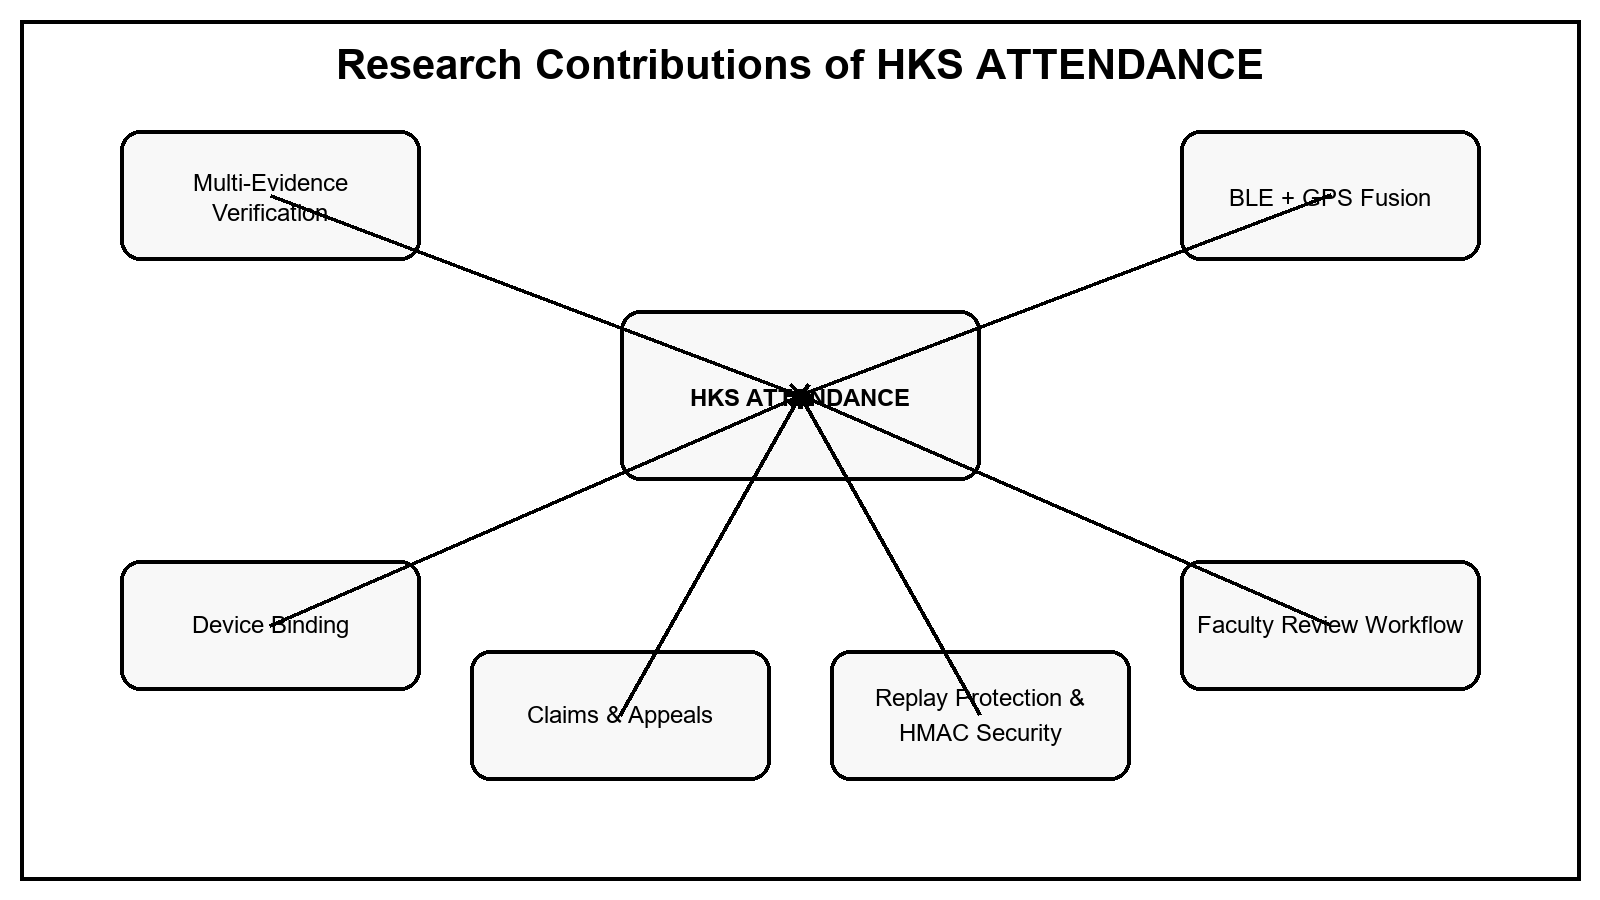
\includegraphics[width=\textwidth,height=0.72\textheight,keepaspectratio]{images/fig1_2_contributions.png}
    \caption{Research Contributions of HKS ATTENDANCE}
    \label{fig:contributions}
\end{figure}


\section{Research Methodology}
\label{sec:methodology}

The project followed a sequential research methodology, illustrated in Figure~\ref{fig:methodology}, moving from problem identification through to evaluation rather than treating design and implementation as a single undifferentiated activity.

\begin{figure}[htbp]
    \centering
    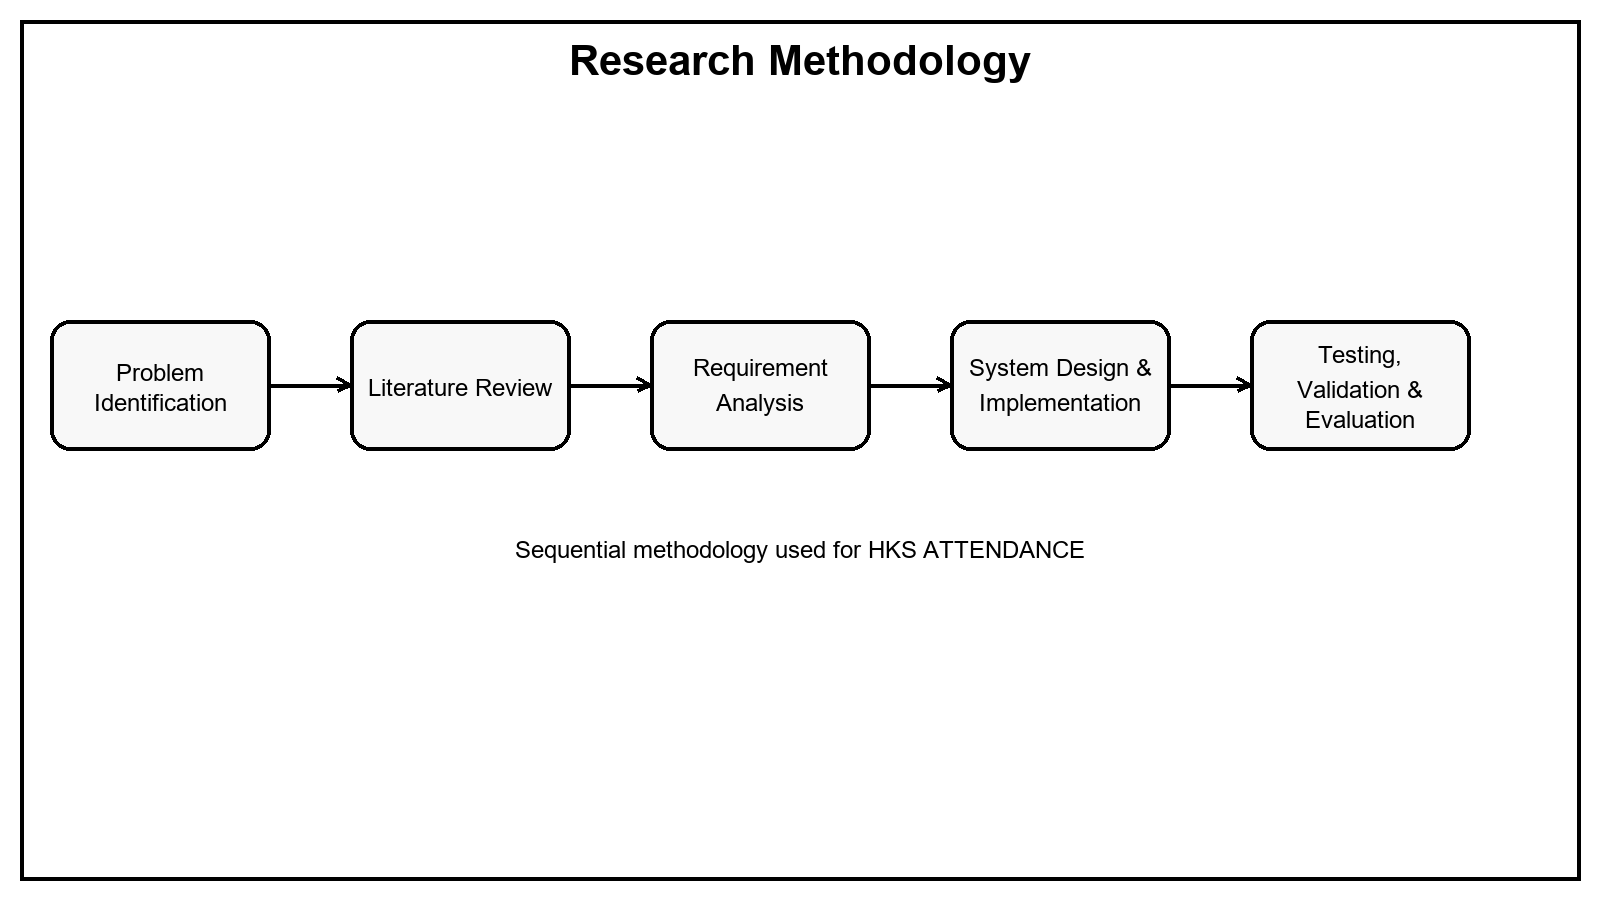
\includegraphics[width=\textwidth,height=0.72\textheight,keepaspectratio]{images/fig1_1_methodology.png}
    \caption{Research Methodology}
    \label{fig:methodology}
\end{figure}


The work began with problem identification: an examination of how attendance is recorded in practice and why existing digital systems continue to be defeated by simple impersonation. This was followed by a literature review covering manual, card-based, code-based, satellite-positioning, biometric, BLE-based, and camera-based approaches, summarised in Chapter~2. The literature review fed directly into a research gap analysis, which identified that very few existing systems combine more than one verification channel, almost none bind a student account to a specific device, and fewer still provide a structured path for faculty review or student appeal.

These gaps shaped the requirement analysis presented in Chapter~3, which translated the identified weaknesses into functional and non-functional requirements. BLE and GPS were selected as the two corroborating evidence channels because they are independently available on commodity smartphones, fail in different and largely unrelated ways, and can be combined without specialised hardware beyond a low-cost beacon. System design (Chapter~4) and database design (Chapter~5) followed, translating these requirements into a layered architecture and a normalised relational schema. Implementation (Chapter~6) produced a working Flutter, FastAPI, and PostgreSQL system together with ESP32 beacon firmware. Testing and validation (Chapter~7) then exercised the system across functional, security, and performance dimensions, and the results were evaluated against the original objectives in Chapter~8 before concluding in Chapter~9.

\subsection{Research Design}
\label{sec:research-design}

Figure~\ref{fig:research-design} restates the methodology of Section~\ref{sec:methodology} as an explicit research-design pipeline, the form in which this kind of sequential, requirements-driven engineering research is typically presented.

\begin{lstlisting}
Problem Identification
        |
        v
Requirement Analysis
        |
        v
Architecture Design
        |
        v
Implementation
        |
        v
Validation
        |
        v
Evaluation
\end{lstlisting}

\begin{figure}[htbp]
    \centering
    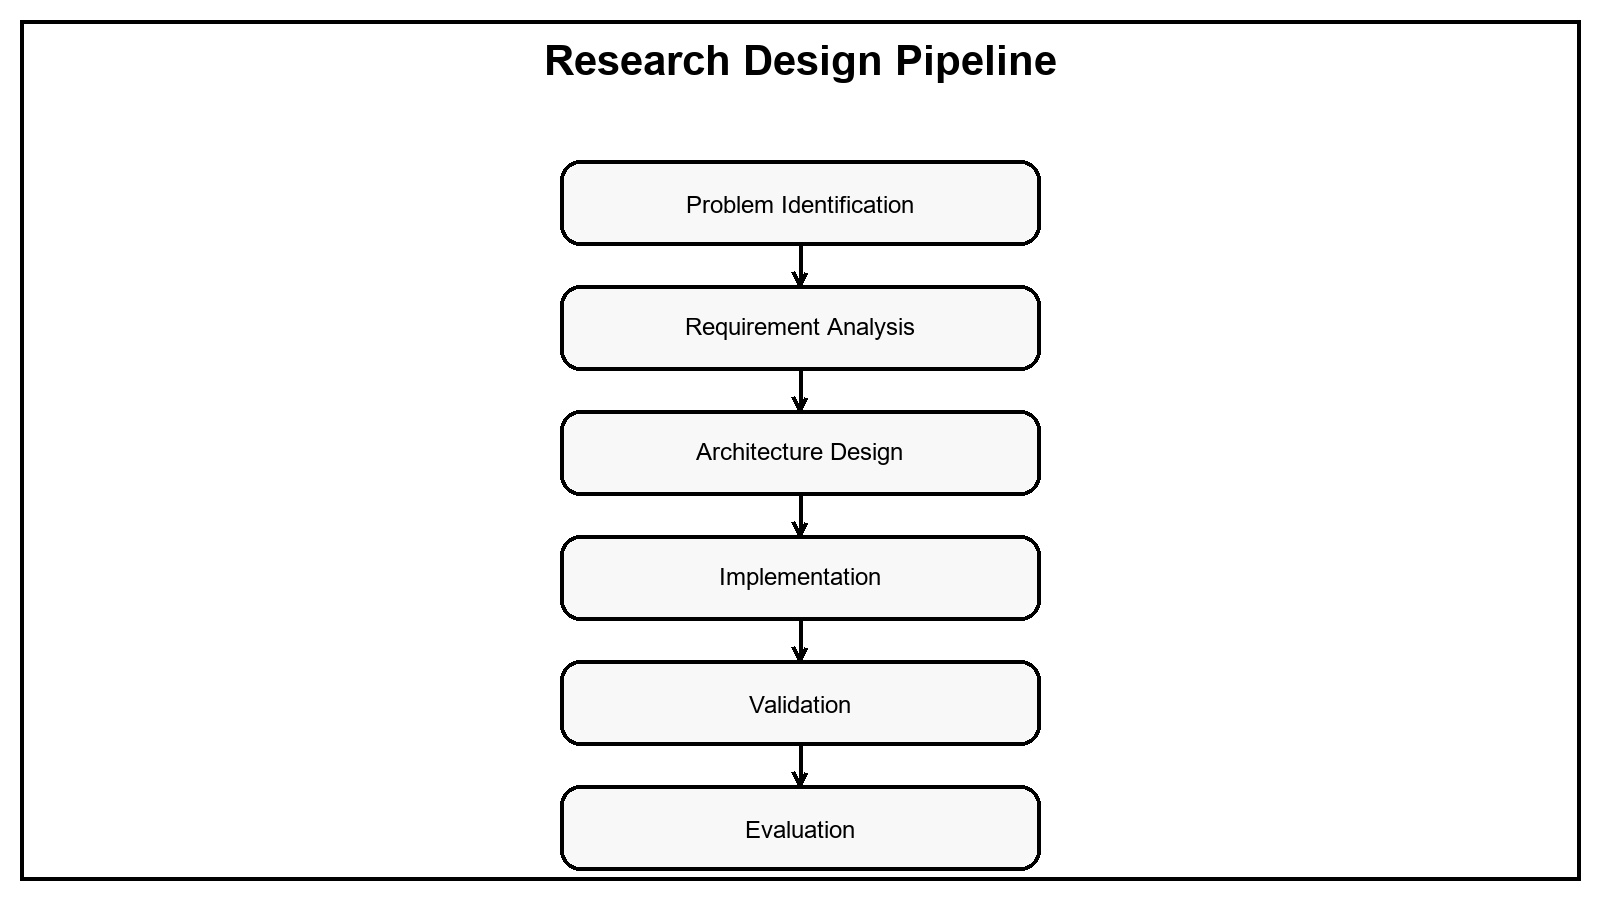
\includegraphics[width=\textwidth,height=0.72\textheight,keepaspectratio]{images/fig1_3_research_design.png}
    \caption{Research Design Pipeline}
    \label{fig:research-design}
\end{figure}


Each stage in this pipeline corresponds directly to a chapter of this thesis: problem identification and requirement analysis are addressed in Chapters~2 and~3, architecture design in Chapters~4 and~5, implementation in Chapter~6, validation in Chapter~7, and evaluation in Chapter~8.

\section{Organisation of the Thesis}
\label{sec:organisation}

The remainder of this thesis is structured as follows. Chapter~2 surveys existing approaches to attendance automation and positions this project relative to them. Chapter~3 presents the system analysis, including requirements and feasibility. Chapter~4 describes the system architecture and module-level design. Chapter~5 covers the database design. Chapter~6 details the implementation of each subsystem, including deployment architecture and threat modelling. Chapter~7 presents the testing and validation methodology and results. Chapter~8 discusses outcomes, comparative positioning, implementation footprint, and limitations. Chapter~9 concludes the thesis and outlines future work.

\section{Chapter Summary}
\label{sec:ch1-summary}

This chapter introduced the problem of single-channel attendance verification, the motivation for combining BLE and GPS evidence, the project's objectives and scope, its principal contributions, the research methodology followed, and the organisation of the remaining chapters. The next chapter presents the literature review that informed the design of HKS ATTENDANCE.

% =============================================================================
% CHAPTER 2: LITERATURE REVIEW
% =============================================================================
\chapter{Literature Review}
\label{chap:literature}

\section{Introduction}

Before settling on a hybrid BLE-and-GPS architecture, it is necessary to examine the broader landscape of attendance-automation technologies that have been studied and deployed over the past two decades, including those this project deliberately did not build on. This chapter reviews manual registers, card-based systems, code-scanning systems, satellite-positioning systems, biometric systems, short-range radio systems, and camera-based recognition systems; it then reviews a representative set of research papers addressing BLE- and GPS-based attendance verification, before positioning HKS ATTENDANCE relative to the gaps identified. Sections~2.3 through~2.5 and~2.8 describe technologies that do not form part of the system implemented in this project; they are reviewed solely as prior art.

\section{Manual Attendance Registers}

The oldest and still most common approach is for an instructor to call a roll and mark a paper or spreadsheet register by hand. This method requires no infrastructure and no training, but it scales poorly with class size, consumes teaching time, and offers no resistance to a student answering on a classmate's behalf. Manual registers are also difficult to audit: once a mark is made, there is rarely a record of the basis on which it was made, and disputed entries are difficult to revisit months later.

\section{Card-Based (RFID) Systems}

Radio-Frequency Identification readers were among the first automated alternatives to the paper register. Each student is issued a card carrying a unique identifier, and a reader installed at the classroom entrance logs a tap as an attendance event. This reduces manual effort and can process a queue of students quickly, but the underlying weakness is structural: a card is a bearer credential, and nothing prevents one student from carrying a friend's card through the reader. Equipping every classroom with reader hardware also adds a recurring infrastructure and maintenance cost that scales with institution size.

\section{Code-Scanning Systems}

A lighter-weight alternative that gained popularity with the spread of smartphones is the display of a time-limited scannable code at the start of a session, which students photograph to register presence. This requires no dedicated hardware beyond a projector and a phone camera. The same lightness, however, undermines it as a verification mechanism: a code displayed on a screen can be photographed and forwarded to anyone, and scanning it does not establish physical presence in the room. Static or long-lived codes are particularly susceptible to this kind of sharing, and even short-lived codes do little to confirm that the scanning device is physically present rather than relying on a forwarded screenshot.

\section{Satellite-Positioning (GPS-Only) Systems}

Systems that rely solely on a device's reported GPS coordinates check those coordinates against a geographic boundary drawn around the institution or a particular building. This requires no additional hardware, since location services are already present on virtually every smartphone, but satellite positioning was not designed for indoor, room-level precision. Signal degradation inside buildings, multipath reflection in dense surroundings, and the relative ease of installing a mock-location utility on a rooted device combine to make GPS, used alone, a weak basis for a presence claim. It can usually confirm that a phone is somewhere on or near a campus; it struggles to confirm which classroom that phone is in, or whether the reported coordinates are genuine.

\section{Biometric Systems}

Fingerprint, iris, and facial-recognition systems verify identity through a physiological trait rather than a possession (a card) or a secret (a password), making casual impersonation considerably harder. The trade-offs are correspondingly larger: dedicated sensors are expensive to deploy at institutional scale, the collection and storage of biometric templates raises privacy and consent questions, and recognition accuracy is sensitive to lighting, sensor quality, and changes in appearance. These costs have kept biometric attendance from becoming the default choice outside higher-stakes or smaller-scale deployments.

\section{Bluetooth Low Energy Proximity Systems}

Bluetooth Low Energy beacons broadcast a short, periodic radio signal that nearby devices can detect and use to estimate proximity. Because BLE is short-range, it performs better than satellite positioning at distinguishing one room from an adjacent one, while drawing very little power, allowing a beacon to run for months on simple hardware. Used alone, however, BLE has its own gaps: received signal strength is noisy and fluctuates with body position and obstruction, an unauthorised device could imitate a legitimate beacon's identifier, and a captured broadcast could be recorded and replayed later unless the protocol explicitly guards against it. These observations directly motivated the security hardening -- nonce validation, nonce caching, and signature verification -- built into the BLE evidence pipeline described in Chapters~4 and~6.

\section{Camera-Based Facial Recognition Systems}

Advances in computer vision have made passive, camera-driven facial recognition a candidate for attendance automation: a camera mounted in a classroom can, in principle, log presence without requiring any action from the student. The cost of that convenience is a substantial compute and camera-infrastructure requirement, sensitivity to lighting and occlusion, and a more pronounced version of the privacy concerns already associated with biometric systems generally, since continuous video capture of a room is a larger intrusion than a single fingerprint scan at the door.

\section{Hybrid and Multi-Evidence Approaches}

A recurring theme in recent research is that no single sensing modality is individually sufficient, and that pairing two complementary, independently weak signals tends to outperform either signal alone. Reported combinations include radio proximity paired with satellite positioning, and biometric verification paired with location checks. The reported benefits are consistent: an attacker must defeat two independent mechanisms rather than one, and the resulting evidence trail is richer, which makes after-the-fact review and dispute resolution more tractable. The corresponding costs are increased architectural complexity, the need to reconcile evidence arriving through different channels, and a greater governance burden, since a hybrid system inevitably produces ambiguous cases that a single-signal system would simply accept or reject outright. HKS ATTENDANCE adopts this hybrid approach directly, pairing BLE proximity evidence with GPS geofence evidence and routing ambiguous cases to a human reviewer rather than resolving them automatically.

\section{Comparison with Commercial Attendance Systems}
\label{sec:commercial-comparison}

In addition to the academic literature reviewed in Sections~2.3 through~2.9, it is useful to position HKS ATTENDANCE against the commercial and off-the-shelf attendance products that institutions encounter in practice. Table~\ref{tab:commercial-comparison} summarises five commonly deployed commercial product categories -- RFID-based attendance terminals, QR/scannable-code attendance apps, consumer GPS-geofencing attendance apps, commercial face-recognition attendance kiosks, and standalone BLE beacon attendance apps -- against the same capability set used in the research gap analysis of Section~2.12.

\begin{table}[p]
\centering
\caption{Comparison with Commercial Attendance Systems}
\label{tab:commercial-comparison}
\scriptsize
\setlength{\tabcolsep}{2.5pt}
\renewcommand{\arraystretch}{1.1}
\resizebox{\textwidth}{!}{%
\begin{tabular}{|p{4.3cm}|c|c|c|c|c|}
\hline
\textbf{Capability} & \textbf{RFID} & \textbf{QR} & \textbf{GPS} & \textbf{Face Rec.} & \textbf{BLE} \\
\hline
Hardware cost & High (reader per room) & Low & None & Very high (camera + compute) & Low (beacon per room) \\
\hline
Resistant to credential sharing & No & No & No & Partially & No \\
\hline
Resistant to replay & N/A & No & No & N/A & Rarely \\
\hline
Indoor room-level precision & Yes & N/A & No & Yes & Yes \\
\hline
Privacy footprint & Low & Low & Moderate & High & Low \\
\hline
Faculty review of evidence & Rarely & Rarely & Rarely & Rarely & Rarely \\
\hline
Dispute / appeal workflow & No & No & No & No & No \\
\hline
\end{tabular}%
}
\end{table}

Commercial RFID terminals and face-recognition kiosks both achieve good room-level precision, but at a hardware cost and (for face recognition) a privacy cost that is difficult to justify for general classroom use. Commercial QR and GPS apps minimise hardware cost but reintroduce the sharing and spoofing weaknesses discussed in Sections~2.4 and~2.6. None of the commercial categories surveyed combine two independent evidence channels, bind a student to a specific device, or expose a faculty-facing evidence-review and appeals workflow -- the same gap identified against the academic literature in Section~2.12, reinforcing that this is a gap in current practice generally and not only in the research literature.

\section{Summary of Literature Findings}

Before turning to a formal gap analysis, it is useful to state plainly what the literature reviewed in Sections~2.2 through~2.10 collectively shows. Five findings recur across the sources surveyed:

\begin{enumerate}
    \item \textbf{Finding 1} -- Most deployed attendance systems rely on a single verification method, whether a card, a code, a location reading, or a biometric trait, and inherit that method's specific weakness wholesale.
    \item \textbf{Finding 2} -- BLE provides meaningfully better indoor proximity resolution than GPS, but is itself vulnerable to signal noise, beacon spoofing, and replay unless explicitly hardened.
    \item \textbf{Finding 3} -- GPS alone cannot reliably distinguish one classroom from an adjacent one, and is comparatively easy to falsify on a rooted or jailbroken device.
    \item \textbf{Finding 4} -- Faculty governance -- a human reviewer inspecting raw evidence before a decision is finalised -- is rarely discussed or implemented in the systems reviewed, academic or commercial.
    \item \textbf{Finding 5} -- Device binding, in the sense of tying a student's attendance privileges to one specific registered device, is almost entirely absent from the literature, despite credential sharing being a frequently cited weakness.
\end{enumerate}

These five findings, taken together, motivate the research gap analysis that follows.

\section{Evolution of Attendance Systems}

Figure~\ref{fig:evolution} places the technologies reviewed in this chapter on a rough timeline, showing the progression from manual registers through card- and code-based systems to location- and proximity-aware approaches, culminating in the multi-evidence design adopted by HKS ATTENDANCE.

\begin{figure}[htbp]
    \centering
    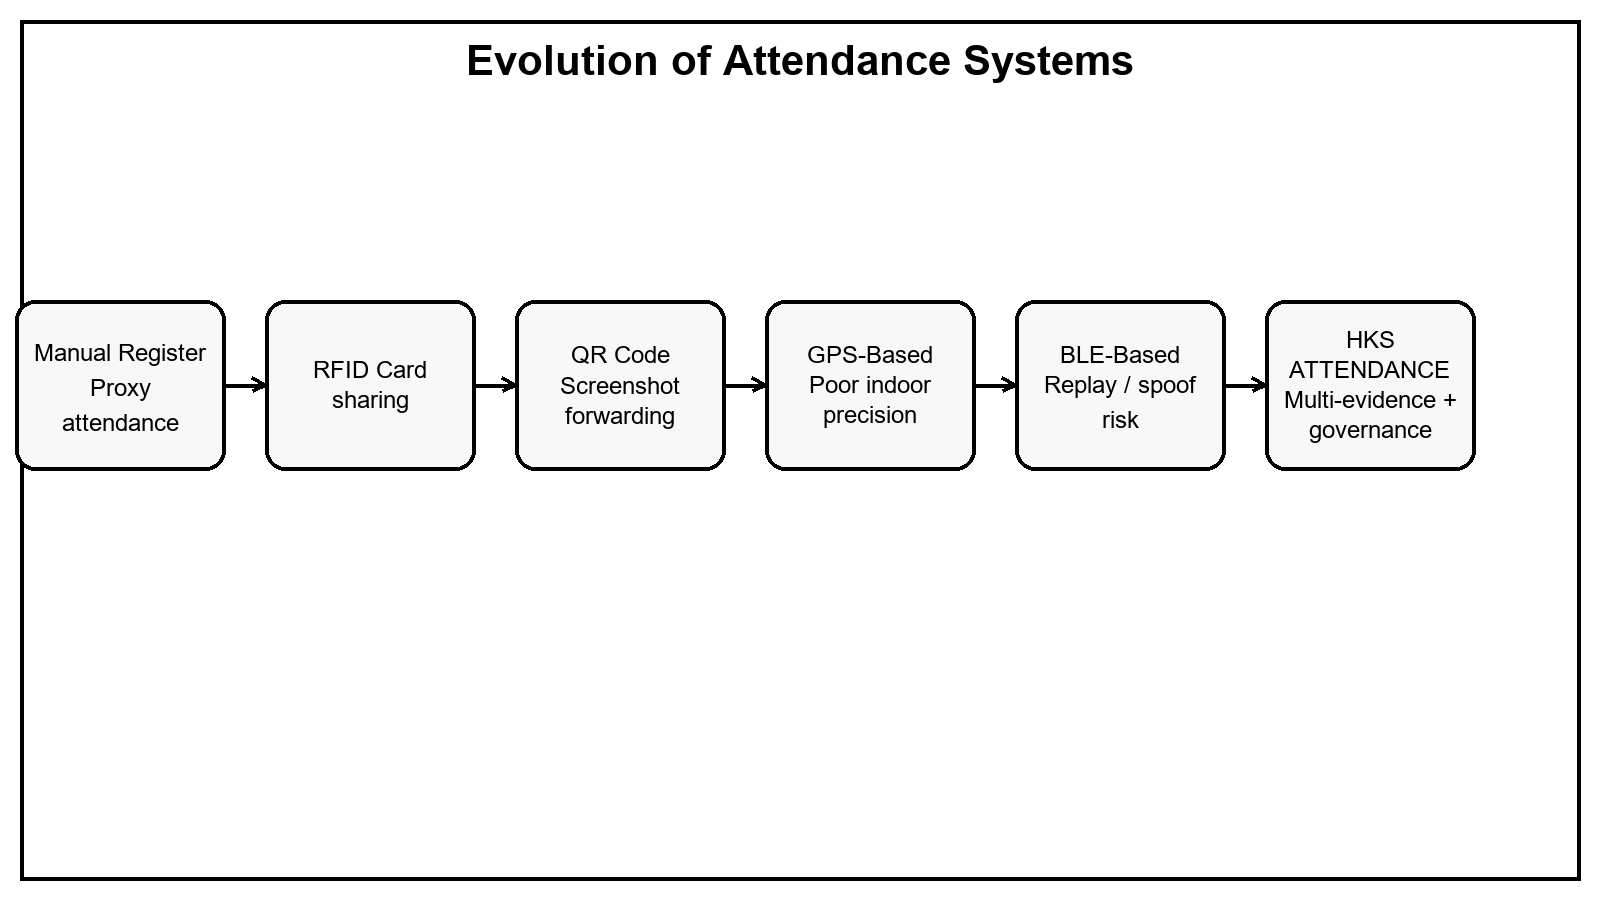
\includegraphics[width=\textwidth,height=0.72\textheight,keepaspectratio]{images/fig2_1_evolution.png}
    \caption{Evolution of Attendance Systems}
    \label{fig:evolution}
\end{figure}


\section{Research Gap Analysis}

Table~\ref{tab:limitation-by-tech} summarises the principal weakness associated with each approach reviewed in Sections~2.2 through~2.8.

\begin{table}[htbp]
\centering
\caption{Principal Limitation by Attendance Technology}
\label{tab:limitation-by-tech}
\begin{tabularx}{\textwidth}{|l|X|}
\hline
\textbf{Technology} & \textbf{Principal Limitation} \\
\hline
Manual Register & No resistance to one student answering for another \\
\hline
RFID Card & Cards are freely transferable between students \\
\hline
Scannable Code & Codes can be photographed and forwarded remotely \\
\hline
GPS Only & Poor indoor precision; coordinates can be falsified \\
\hline
Biometric & High deployment cost; privacy and consent concerns \\
\hline
BLE Only & Signal noise; vulnerable to beacon spoofing and replay \\
\hline
Facial Recognition & Camera infrastructure cost; privacy intrusion \\
\hline
\end{tabularx}
\end{table}

Table~\ref{tab:limitation-by-tech} compares technologies by their single principal weakness. Table~\ref{tab:comparison-existing} extends this into a broader, multi-feature comparison across the eleven capabilities most relevant to this thesis, making explicit just how many of these capabilities are absent from each existing approach.

\begin{table}[htbp]
\centering
\caption{Comparison Between Existing Systems and HKS ATTENDANCE}
\label{tab:comparison-existing}
\scriptsize
\setlength{\tabcolsep}{2.5pt}
\renewcommand{\arraystretch}{1.1}
\resizebox{\textwidth}{!}{%
\begin{tabular}{|p{3.8cm}|c|c|c|c|c|}
\hline
\textbf{Feature} & \textbf{RFID} & \textbf{QR} & \textbf{GPS} & \textbf{BLE} & \textbf{HKS} \\
\hline
Device Binding & No & No & No & No & Yes \\
\hline
Faculty Review & No & No & No & No & Yes \\
\hline
Claims / Appeals & No & No & No & No & Yes \\
\hline
Audit Logging & No & No & No & No & Yes \\
\hline
Replay Protection & N/A & No & No & No & Yes \\
\hline
Nonce Validation & N/A & No & No & No & Yes \\
\hline
GPS Evidence & No & No & Yes & No & Yes \\
\hline
BLE Evidence & No & No & No & Yes & Yes \\
\hline
JWT-Based Auth. & No & No & No & No & Yes \\
\hline
Administrative Governance & Limited & No & Limited & Limited & Yes \\
\hline
Cloud Deployment & Rarely & Rarely & Sometimes & Rarely & Yes \\
\hline
\end{tabular}%
}
\end{table}

The pattern in Table~\ref{tab:comparison-existing} is consistent with Table~\ref{tab:limitation-by-tech}: existing single-channel technologies each cover at most two or three of the eleven capabilities considered, while HKS ATTENDANCE was deliberately designed to cover all eleven simultaneously.

\section{Review of Related Research Papers}

To situate HKS ATTENDANCE within the published research on attendance automation, Table~\ref{tab:reviewed-papers} summarises twelve representative papers and standards spanning BLE proximity systems, GPS-based systems, multi-factor and hybrid verification schemes, and the underlying wireless and cryptographic primitives the project draws on. Full bibliographic details for each entry, together with the remaining references consulted during the project, appear in the References section at the end of this thesis.

\begin{table}[p]
\centering
\caption{Summary of Reviewed Research Papers}
\label{tab:reviewed-papers}
\tiny
\setlength{\tabcolsep}{3pt}
\renewcommand{\arraystretch}{1.08}
\begin{tabularx}{\textwidth}{|>{\centering\arraybackslash}p{0.55cm}|X|X|X|X|}
\hline
\textbf{\#} & \textbf{Focus Area} & \textbf{Methodology} & \textbf{Reported Advantage} & \textbf{Reported Limitation} \\
\hline
1 & BLE-based attendance management~\cite{ref1} & Fixed BLE beacons paired with a mobile scanning application & Removes manual roll-call effort; low beacon power draw & No device-binding or replay protection described \\
\hline
2 & Smart attendance using BLE~\cite{ref2} & RSSI-threshold proximity detection & Improves on RFID by removing the bearer-card problem & Signal strength alone reported as noisy and position-sensitive \\
\hline
3 & GPS-based attendance for mobile devices~\cite{ref3} & Geofence radius check against a single registered campus location & No additional hardware required & Cannot distinguish adjacent rooms; vulnerable to location spoofing \\
\hline
4 & Multi-factor secure attendance~\cite{ref4} & Combines a password factor with a location factor & Reduces simple credential sharing & Does not address device binding or proximity verification \\
\hline
5 & Survey of wireless attendance technologies~\cite{ref5} & Comparative literature survey & Identifies that no single wireless technology is sufficient alone & Survey-level; does not implement a combined system \\
\hline
6 & Bluetooth Core Specification~\cite{ref6} & Protocol-level specification of BLE advertising behaviour & Defines the low-power advertising model the project's beacons rely on & Specification only; no application-layer security guidance \\
\hline
7 & ESP32 technical reference~\cite{ref7,ref8} & Hardware and firmware reference for ESP32-class microcontrollers & Establishes feasibility of low-cost, long-running beacon hardware & Does not address attendance-specific payload design \\
\hline
8 & Bluetooth/Wi-Fi interference study~\cite{ref9} & Simulation of 802.11 and Bluetooth coexistence & Quantifies expected interference in shared 2.4~GHz environments & Does not address spoofing or replay threats \\
\hline
9 & Mobile location services documentation~\cite{ref10,ref11} & Platform-level GPS and fused-location APIs & Provides accuracy and freshness metadata usable for evidence quality checks & Documentation rather than a verification scheme \\
\hline
10 & HMAC keyed-hashing specification~\cite{ref16} & Cryptographic primitive for message authentication & Provides the signature mechanism used to authenticate beacon payloads & Generic primitive; requires application-specific key and nonce management \\
\hline
11 & JSON Web Token specification~\cite{ref17} & Token-based authentication standard & Provides a stateless, verifiable session credential & Does not address device binding or proximity verification \\
\hline
12 & OWASP API Security Top 10~\cite{ref15} & Catalogue of common API security weaknesses & Used to validate the security posture of the REST interface & General-purpose; not specific to attendance systems \\
\hline
\end{tabularx}
\end{table}

Across this body of work, very few systems combine more than one verification channel, almost none bind a student account to a specific device, and fewer still provide a structured path for a student to contest a rejected record or allow faculty to inspect the underlying evidence before a decision is finalised. Table~\ref{tab:gap-matrix} expresses this comparison as a feature-coverage matrix.

\begin{table}[htbp]
\centering
\caption{Research Gap Matrix}
\label{tab:gap-matrix}
\small
\setlength{\tabcolsep}{4pt}
\begin{tabularx}{\textwidth}{|X|c|c|c|c|c|}
\hline
\textbf{System / Approach} & \textbf{BLE} & \textbf{GPS} & \textbf{Device Binding} & \textbf{Faculty Review} & \textbf{Claims Resolution} \\
\hline
Manual Register & No & No & No & No & No \\
\hline
RFID Card Reader & No & No & No & No & No \\
\hline
Scannable Code & No & No & No & No & No \\
\hline
GPS-Only Mobile App & No & Yes & No & No & No \\
\hline
BLE-Only Mobile App~\cite{ref1,ref2} & Yes & No & No & No & No \\
\hline
Multi-Factor Scheme~\cite{ref4} & No & Limited & No & No & No \\
\hline
HKS ATTENDANCE (this work) & Yes & Yes & Yes & Yes & Yes \\
\hline
\end{tabularx}
\end{table}

\section{Observations Arising from the Research Gap Analysis}

Reading Tables~\ref{tab:limitation-by-tech} through~\ref{tab:gap-matrix} together yields five specific observations that directly shaped the requirements presented in Chapter~3:

\begin{enumerate}
    \item \textbf{Observation 1} -- No reviewed system combines BLE and GPS evidence in a single, jointly evaluated decision; where both are present, they are typically used as alternatives rather than as corroborating signals.
    \item \textbf{Observation 2} -- Device binding is essentially absent from the literature reviewed, despite credential and card sharing being the most frequently cited weakness of existing systems.
    \item \textbf{Observation 3} -- Faculty governance, in the sense of a human reviewer inspecting raw evidence before a decision is finalised, appears in very few systems; most either accept or reject automatically.
    \item \textbf{Observation 4} -- A structured claims or appeals workflow is rarely implemented, leaving students with no formal recourse when an automated decision is incorrect.
    \item \textbf{Observation 5} -- Replay protection for wireless evidence (BLE or otherwise) is largely absent from the attendance-specific literature, even though it is a well-understood requirement in the broader wireless-security literature.
\end{enumerate}

Each of these five observations maps directly onto one of the six design choices listed in Section~2.16, and onto the functional requirements set out in Chapter~3.

\section{Positioning of HKS ATTENDANCE}

HKS ATTENDANCE responds to the gaps identified above through six design choices acting together rather than in isolation:

\begin{itemize}
    \item Attendance decisions are derived jointly from BLE proximity evidence and GPS geofence evidence, rather than from either alone.
    \item Every attendance submission is tied to a single device registered against the submitting student's account.
    \item Beacon broadcasts are protected with single-use nonces, freshness checks, and cryptographic signatures to resist replay and spoofing.
    \item Submissions that the automated decision engine cannot confidently accept or reject are routed to the responsible faculty member for evidence-based review.
    \item Administrative tooling manages the full academic hierarchy -- users, courses, enrolments, classrooms, and trusted beacons -- as a first-class part of the platform.
    \item Students may formally contest a rejected attendance record, with the outcome and reasoning permanently logged.
\end{itemize}

\section{Chapter Summary}

This chapter reviewed the principal technologies used or proposed for automated attendance -- registers, RFID, scannable codes, GPS, biometrics, BLE, facial recognition, and combinations thereof -- together with a representative set of published research papers and standards addressing BLE- and GPS-based verification, and positioned HKS ATTENDANCE against a representative set of commercial attendance products. Five specific observations were drawn from the resulting gap analysis, and a consistent pattern emerged: systems built around a single evidence channel inherit that channel's specific weakness, while hybrid designs trade implementation complexity for stronger resistance to manipulation. The next chapter translates these observations into a concrete set of functional and non-functional requirements for HKS ATTENDANCE.

% =============================================================================
% CHAPTER 3: SYSTEM ANALYSIS
% =============================================================================
\chapter{System Analysis}
\label{chap:analysis}

\section{Introduction}

Before development began, the project required a clear analysis of what existing attendance practices fail to deliver, which of those failures a new system could realistically address, and what a workable solution would need to do in concrete, testable terms. This chapter presents that analysis: the shortcomings of current practice, the requirements they imply, a feasibility assessment across technical, economic, operational, and scheduling dimensions, and the constraints and assumptions under which the system was designed and built.

\section{Shortcomings of Current Practice}

\subsection{Impersonation}
The most persistent problem in attendance recording is one student marking presence on behalf of an absent classmate. Manual registers offer no defence against this, and many digitised systems do little better, since a shared credential, a borrowed card, or a forwarded screenshot reproduces the same failure in a different form.

\subsection{Single-Channel Verification}
Most automated systems reviewed in Chapter~2 base the entire attendance decision on one piece of evidence. Once that channel is compromised -- a card is lent, a code is forwarded, a location is spoofed -- there is no remaining basis for the decision.

\subsection{Coarse Location Granularity}
Systems that rely on GPS alone frequently confirm only that a device is somewhere on or near a campus, not that it is in the specific room where a session is taking place. A student outside a lecture hall, or in a neighbouring building under favourable signal conditions, can sometimes register a presence that would not withstand closer scrutiny.

\subsection{Weak Auditability}
When an attendance dispute arises, institutions are frequently unable to reconstruct why a particular decision was made, what evidence supported it, or who reviewed it. Without this trail, disputes tend to be resolved informally rather than on the basis of recorded fact.

\subsection{Absence of Governance Workflow}
Many systems treat attendance as a write-once operation: a submission is accepted or rejected, and that is the end of the matter. There is no path for a faculty member to intervene in an ambiguous case, and no path for a student to formally contest an outcome believed to be wrong.

\subsection{Security Weaknesses}
Common weaknesses observed across the systems reviewed include vulnerability to replayed verification data, ease of sharing credentials or devices between students, the possibility of an unauthorised beacon or reader masquerading as a trusted one, and a lack of enforcement around session validity, allowing attendance to be submitted after a class has ended.

\section{The Case for a New System}

Taken together, these shortcomings point toward a system that verifies physical presence through more than one channel, ties submissions to an authenticated and individually identifiable device, gives faculty visibility into the evidence behind ambiguous decisions, gives students a formal way to contest outcomes, and records every governance action permanently. These requirements directly shaped the design of HKS ATTENDANCE.

\section{Proposed System Overview}

HKS ATTENDANCE bases its attendance decisions on the combination of BLE proximity evidence and GPS geofence evidence, layered with device-binding enforcement, faculty review of ambiguous submissions, administrative governance of the academic hierarchy and beacon infrastructure, and a formal claims process for disputed outcomes.

\section{Architecture at a Glance}

The platform follows a layered design: a Flutter mobile client at the top, communicating over a REST interface with a FastAPI backend, which enforces business rules and security checks before persisting state to a PostgreSQL database. The technology choices are summarised in Table~\ref{tab:core-tech}.

\begin{figure}[htbp]
    \centering
    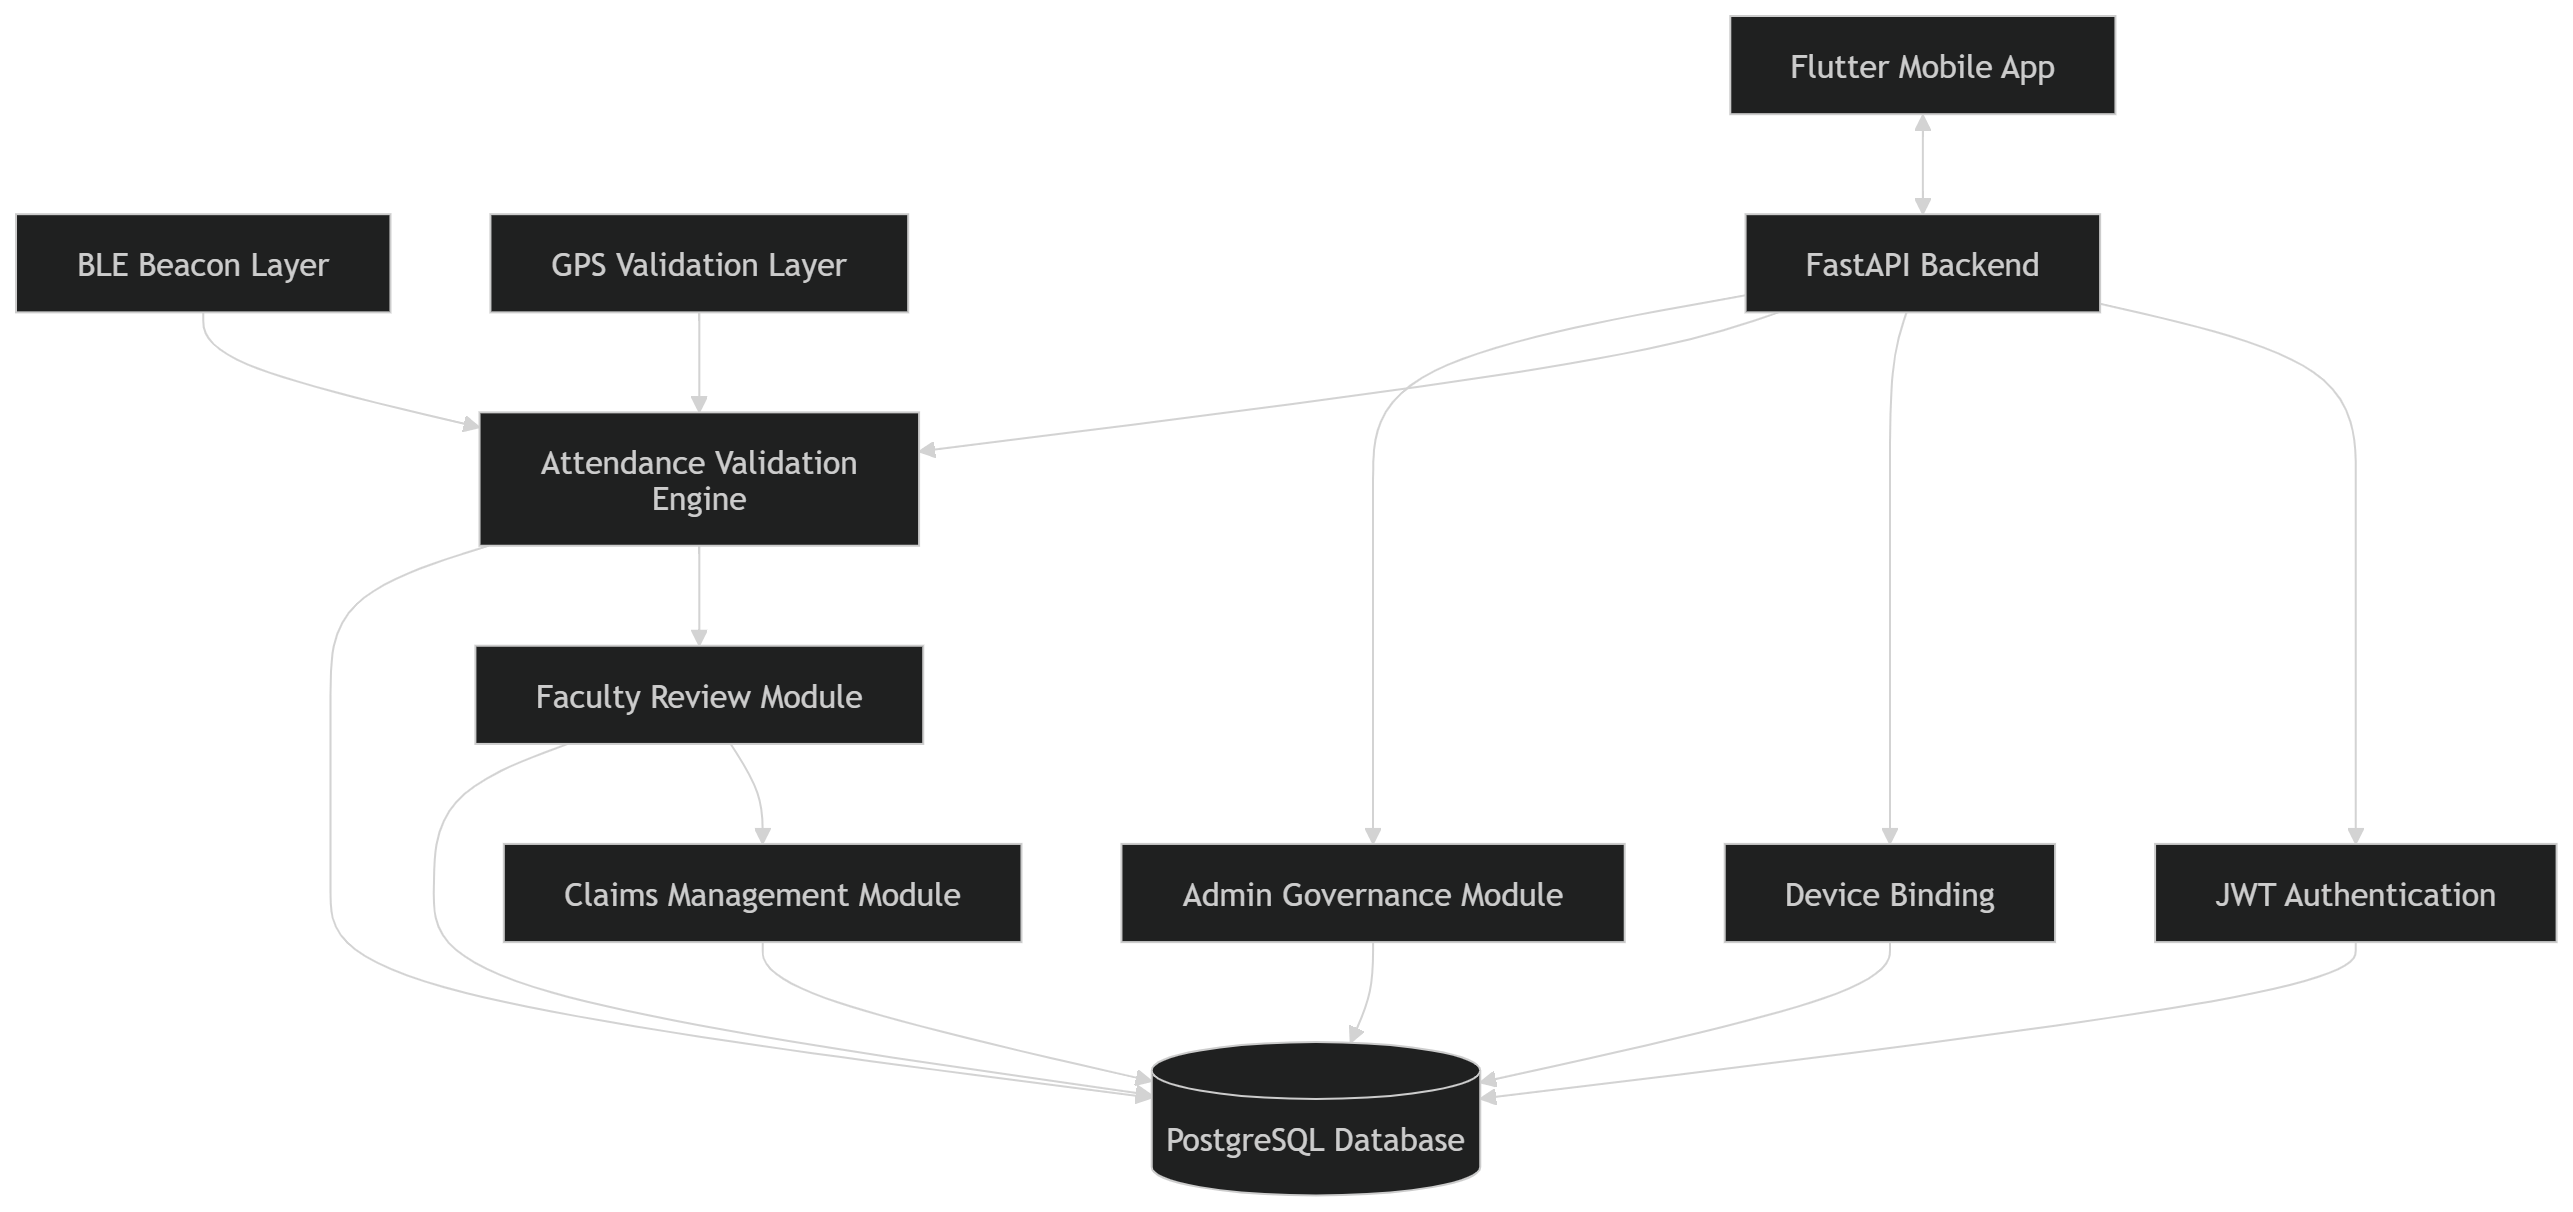
\includegraphics[width=\textwidth,height=0.72\textheight,keepaspectratio]{images/design/architecture/system_architecture.png}
    \caption{Overall System Architecture}
    \label{fig:overall-architecture}
\end{figure}
\textit{Diagram redrawn for this submission from the layer descriptions given throughout Chapters~3--6.}

\begin{table}[htbp]
\centering
\caption{Core Technology Choices}
\label{tab:core-tech}
\begin{tabularx}{\textwidth}{|l|X|}
\hline
\textbf{Layer} & \textbf{Technology} \\
\hline
Mobile Application & Flutter \\
\hline
Backend API & FastAPI \\
\hline
Database & PostgreSQL \\
\hline
BLE Infrastructure & ESP32 microcontrollers \\
\hline
Authentication & JSON Web Tokens (JWT) \\
\hline
\end{tabularx}
\end{table}

\section{Stakeholders and Responsibilities}

\subsection{Student}
\begin{itemize}
    \item Authenticate and discover sessions for enrolled courses.
    \item Collect and submit BLE and GPS evidence to register attendance.
    \item View attendance history and profile information.
    \item Submit claims against rejected attendance records.
\end{itemize}

\subsection{Faculty}
\begin{itemize}
    \item Start, monitor, and close attendance sessions.
    \item Review flagged attendance and inspect supporting evidence.
    \item Confirm or reject ambiguous attendance records.
    \item Review and resolve student claims.
\end{itemize}

\subsection{Administrator}
\begin{itemize}
    \item Manage student and faculty accounts.
    \item Manage courses, faculty-course assignments, and enrolments.
    \item Manage classrooms and the trusted-beacon registry.
    \item Govern device bindings, including unbinding compromised or lost devices.
\end{itemize}

\section{Functional Requirements}

\begin{table}[htbp]
\centering
\caption{Summary of Functional Requirements}
\label{tab:func-req}
\begin{tabularx}{\textwidth}{|l|X|}
\hline
\textbf{ID} & \textbf{Requirement} \\
\hline
FR-1 & Authenticate users and issue session-scoped JWT tokens \\
\hline
FR-2 & Bind a student account to exactly one active device \\
\hline
FR-3 & Surface only active sessions for a student's enrolled courses \\
\hline
FR-4 & Accept BLE and GPS evidence as part of attendance submission \\
\hline
FR-5 & Validate BLE evidence against the trusted-beacon registry \\
\hline
FR-6 & Validate GPS evidence against the relevant classroom geofence \\
\hline
FR-7 & Present flagged attendance records for faculty review \\
\hline
FR-8 & Allow faculty to confirm or reject flagged records \\
\hline
FR-9 & Allow students to submit and track claims; allow faculty to resolve them \\
\hline
FR-10 & Provide administrative CRUD operations over the academic hierarchy \\
\hline
\end{tabularx}
\end{table}

\begin{figure}[htbp]
    \centering
    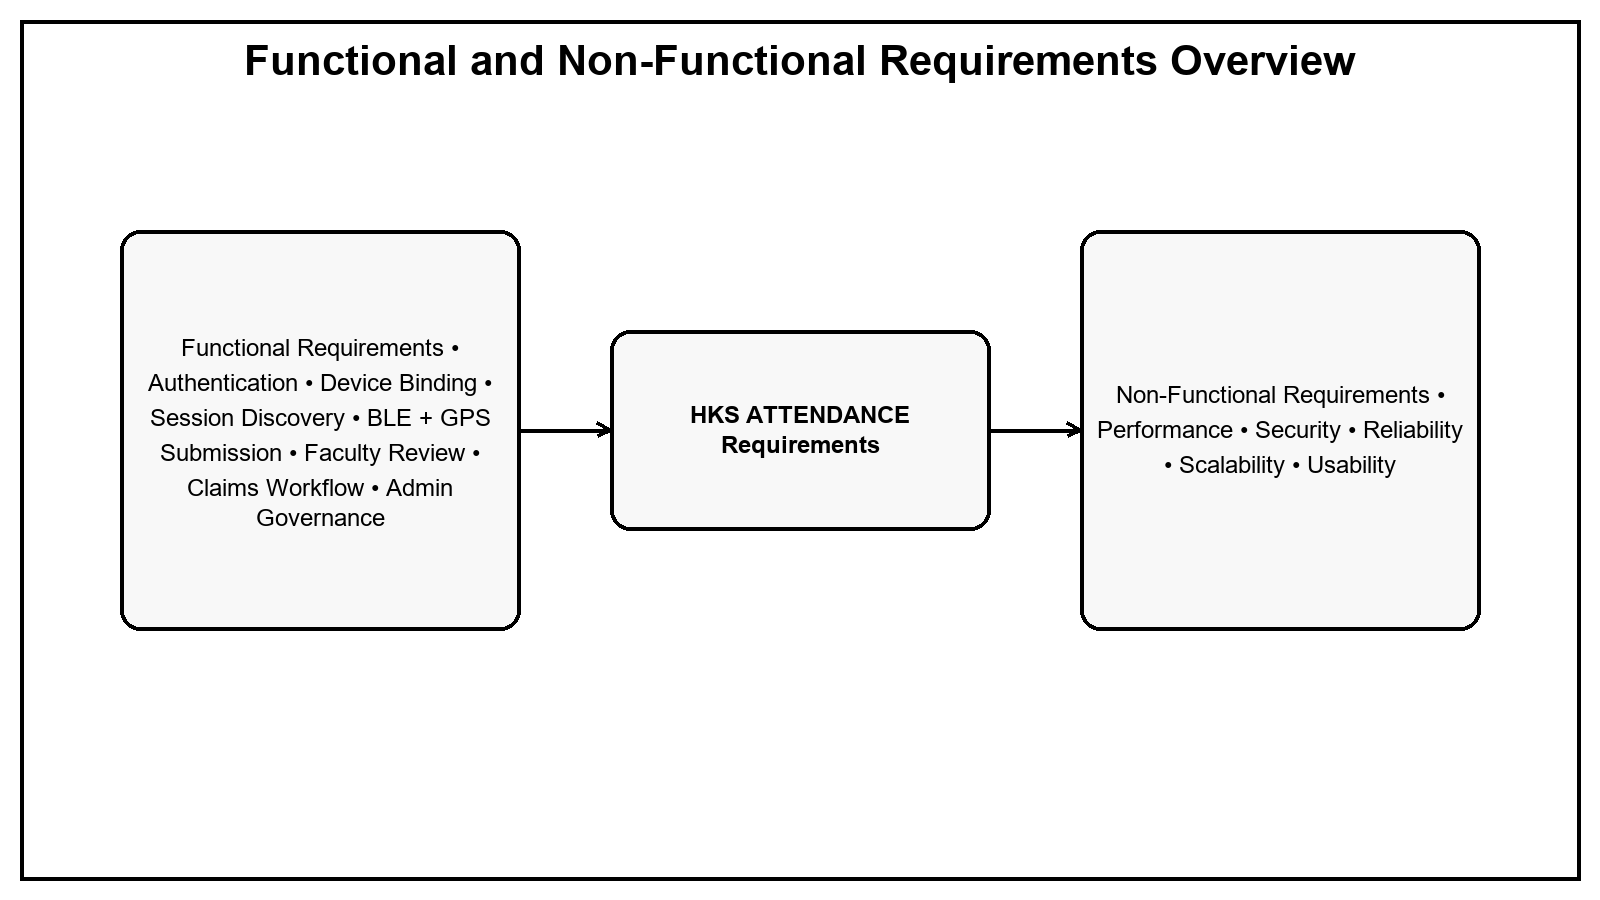
\includegraphics[width=\textwidth,height=0.72\textheight,keepaspectratio]{images/fig3_2_requirements.png}
    \caption{Functional and Non-Functional Requirements Overview}
    \label{fig:requirements-overview}
\end{figure}


\section{Non-Functional Requirements}

\subsection{Performance}
Attendance submission, including evidence validation, was targeted to complete within approximately three seconds under normal operating conditions.

\subsection{Security}
The system must enforce authentication, role-based authorisation, device verification, and protection against replayed evidence.

\subsection{Reliability}
Attendance operations must complete without leaving the database in an inconsistent state, even under concurrent submissions.

\subsection{Scalability}
The schema and architecture must accommodate institutional growth in the number of students, courses, sessions, and historical attendance records without requiring redesign.

\subsection{Usability}
Interfaces for students, faculty, and administrators must remain intuitive enough to require minimal training.

\section{Feasibility Study}

\subsection{Technical Feasibility}
Every technology selected for the project -- Flutter, FastAPI, PostgreSQL, JWT, and ESP32-based BLE firmware -- is mature, well-documented, and widely supported, making the project technically feasible within the available development timeframe.

\subsection{Economic Feasibility}
Beyond the smartphones and network connectivity that students and staff already possess, the only additional hardware required is a small number of inexpensive ESP32 boards per classroom, keeping the marginal deployment cost low relative to card-reader or biometric alternatives.

\subsection{Operational Feasibility}
Each stakeholder group interacts with the system through a role-specific interface -- a student app, a faculty dashboard, and an administrative console -- none of which demands specialised training beyond a short orientation.

\subsection{Schedule Feasibility}
The project was structured into eight sequential phases -- academic-model design, session discovery, the evidence layer, the student-facing product, faculty governance, administrative governance, the claims subsystem, and final validation -- each completed within the academic timeline allotted to the project.

\subsection{Consolidated Feasibility Summary}
Table~\ref{tab:feasibility} consolidates the feasibility assessment across all dimensions considered for the project, including legal and risk considerations not discussed as separate subsections above.

\begin{table}[p]
\centering
\caption{Consolidated Feasibility Summary}
\label{tab:feasibility}
\scriptsize
\setlength{\tabcolsep}{3pt}
\renewcommand{\arraystretch}{1.1}
\resizebox{\textwidth}{!}{%
\begin{tabular}{|p{2.5cm}|p{9.8cm}|p{2.4cm}|}
\hline
\textbf{Dimension} & \textbf{Assessment} & \textbf{Status} \\
\hline
Technical & All selected technologies are mature, well-documented, and within the team's existing skill set. & Feasible \\
\hline
Economic & Marginal hardware cost is limited to inexpensive ESP32 beacons, with no licensing cost for the core stack. & Feasible \\
\hline
Operational & Role-specific interfaces require minimal training for students, faculty, and administrators. & Feasible \\
\hline
Legal & No biometric data is collected; location data is used only transiently for geofence evaluation. & Feasible, subject to institutional policy \\
\hline
Schedule & The eight-phase implementation plan fits within the academic project timeline. & Feasible \\
\hline
Risk & Main risks are beacon misconfiguration and indoor GPS variability, both mitigated by faculty review and validation controls. & Manageable \\
\hline
\end{tabular}%
}
\end{table}

\section{Constraints}
\begin{itemize}
    \item Attendance submission requires an active internet connection.
    \item BLE evidence collection requires properly installed and registered classroom beacons.
    \item GPS evidence collection requires location services to be enabled on the student's device.
    \item Every student is assumed to possess a compatible smartphone.
\end{itemize}

\section{Assumptions}
\begin{itemize}
    \item Classroom coordinates and geofence radii are configured accurately by administrators.
    \item Beacons are installed in the classroom they are registered against and not relocated without an administrative update.
    \item Faculty and administrative accounts are used only by their authorised holders.
\end{itemize}

\section{Anticipated Benefits}
\begin{itemize}
    \item Stronger resistance to impersonation through device binding and dual-channel verification.
    \item Improved auditability through comprehensive evidence and decision logging.
    \item Shared governance between automated checks and human faculty review.
    \item A structured, transparent path for resolving attendance disputes.
\end{itemize}

\section{Chapter Summary}

This chapter analysed the shortcomings of existing attendance practice, translated them into functional and non-functional requirements, and confirmed the technical, economic, operational, and scheduling feasibility of building HKS ATTENDANCE within the available project timeline. The next chapter presents the resulting system design in detail.

% =============================================================================
% CHAPTER 4: SYSTEM DESIGN
% =============================================================================
\chapter{System Design}
\label{chap:design}

\section{Introduction}
This chapter translates the requirements established in Chapter~3 into a concrete architecture: the layering of the system, the technologies bound to each layer, the major functional modules, and the way evidence flows from a student's phone through to a final, faculty-reviewable attendance decision.

\section{Design Principles}

Before describing the architecture itself, it is useful to state the design principles applied consistently across every layer and module of HKS ATTENDANCE:

\begin{itemize}
    \item \textbf{Security by Design} -- authentication, device binding, and evidence validation are treated as core requirements present from the first design iteration, not as features added after a working prototype existed.
    \item \textbf{Evidence Fusion} -- no single signal is ever trusted in isolation; every attendance decision draws on at least two independent evidence sources, as detailed in Section~4.5.
    \item \textbf{Separation of Concerns} -- presentation, business logic, security, and persistence are kept in distinct layers (Section~4.3), so that a change to one (for example, swapping the BLE library used on the client) does not require changes to the others.
    \item \textbf{Least Privilege} -- each role (student, faculty, administrator) is granted only the permissions its tasks require; a faculty member cannot, for instance, act on a course they do not own.
    \item \textbf{Role-Based Access} -- every protected endpoint checks the caller's role and, where relevant, their ownership of the specific resource being acted upon, before performing the requested action.
    \item \textbf{Scalability} -- the schema and architecture are normalised around courses, sessions, and classrooms rather than hard-coded institutional specifics, so that additional courses, classrooms, or even departments can be added without structural change.
    \item \textbf{Modularity} -- the six functional modules introduced in Section~4.6 are designed to evolve largely independently of one another.
\end{itemize}

\section{Layered Architecture}

The system is organised into five layers, each responsible for a distinct concern: the Flutter mobile client at the presentation layer; a FastAPI-based REST interface; a business-services layer implementing attendance, claims, faculty, and administrative logic; a security layer enforcing authentication, BLE and GPS validation, and device checks; and a PostgreSQL persistence layer at the base. Requests flow downward from the mobile client through each layer in turn, with each layer validating only the concerns it owns before handing off to the next.

\begin{figure}[htbp]
    \centering
    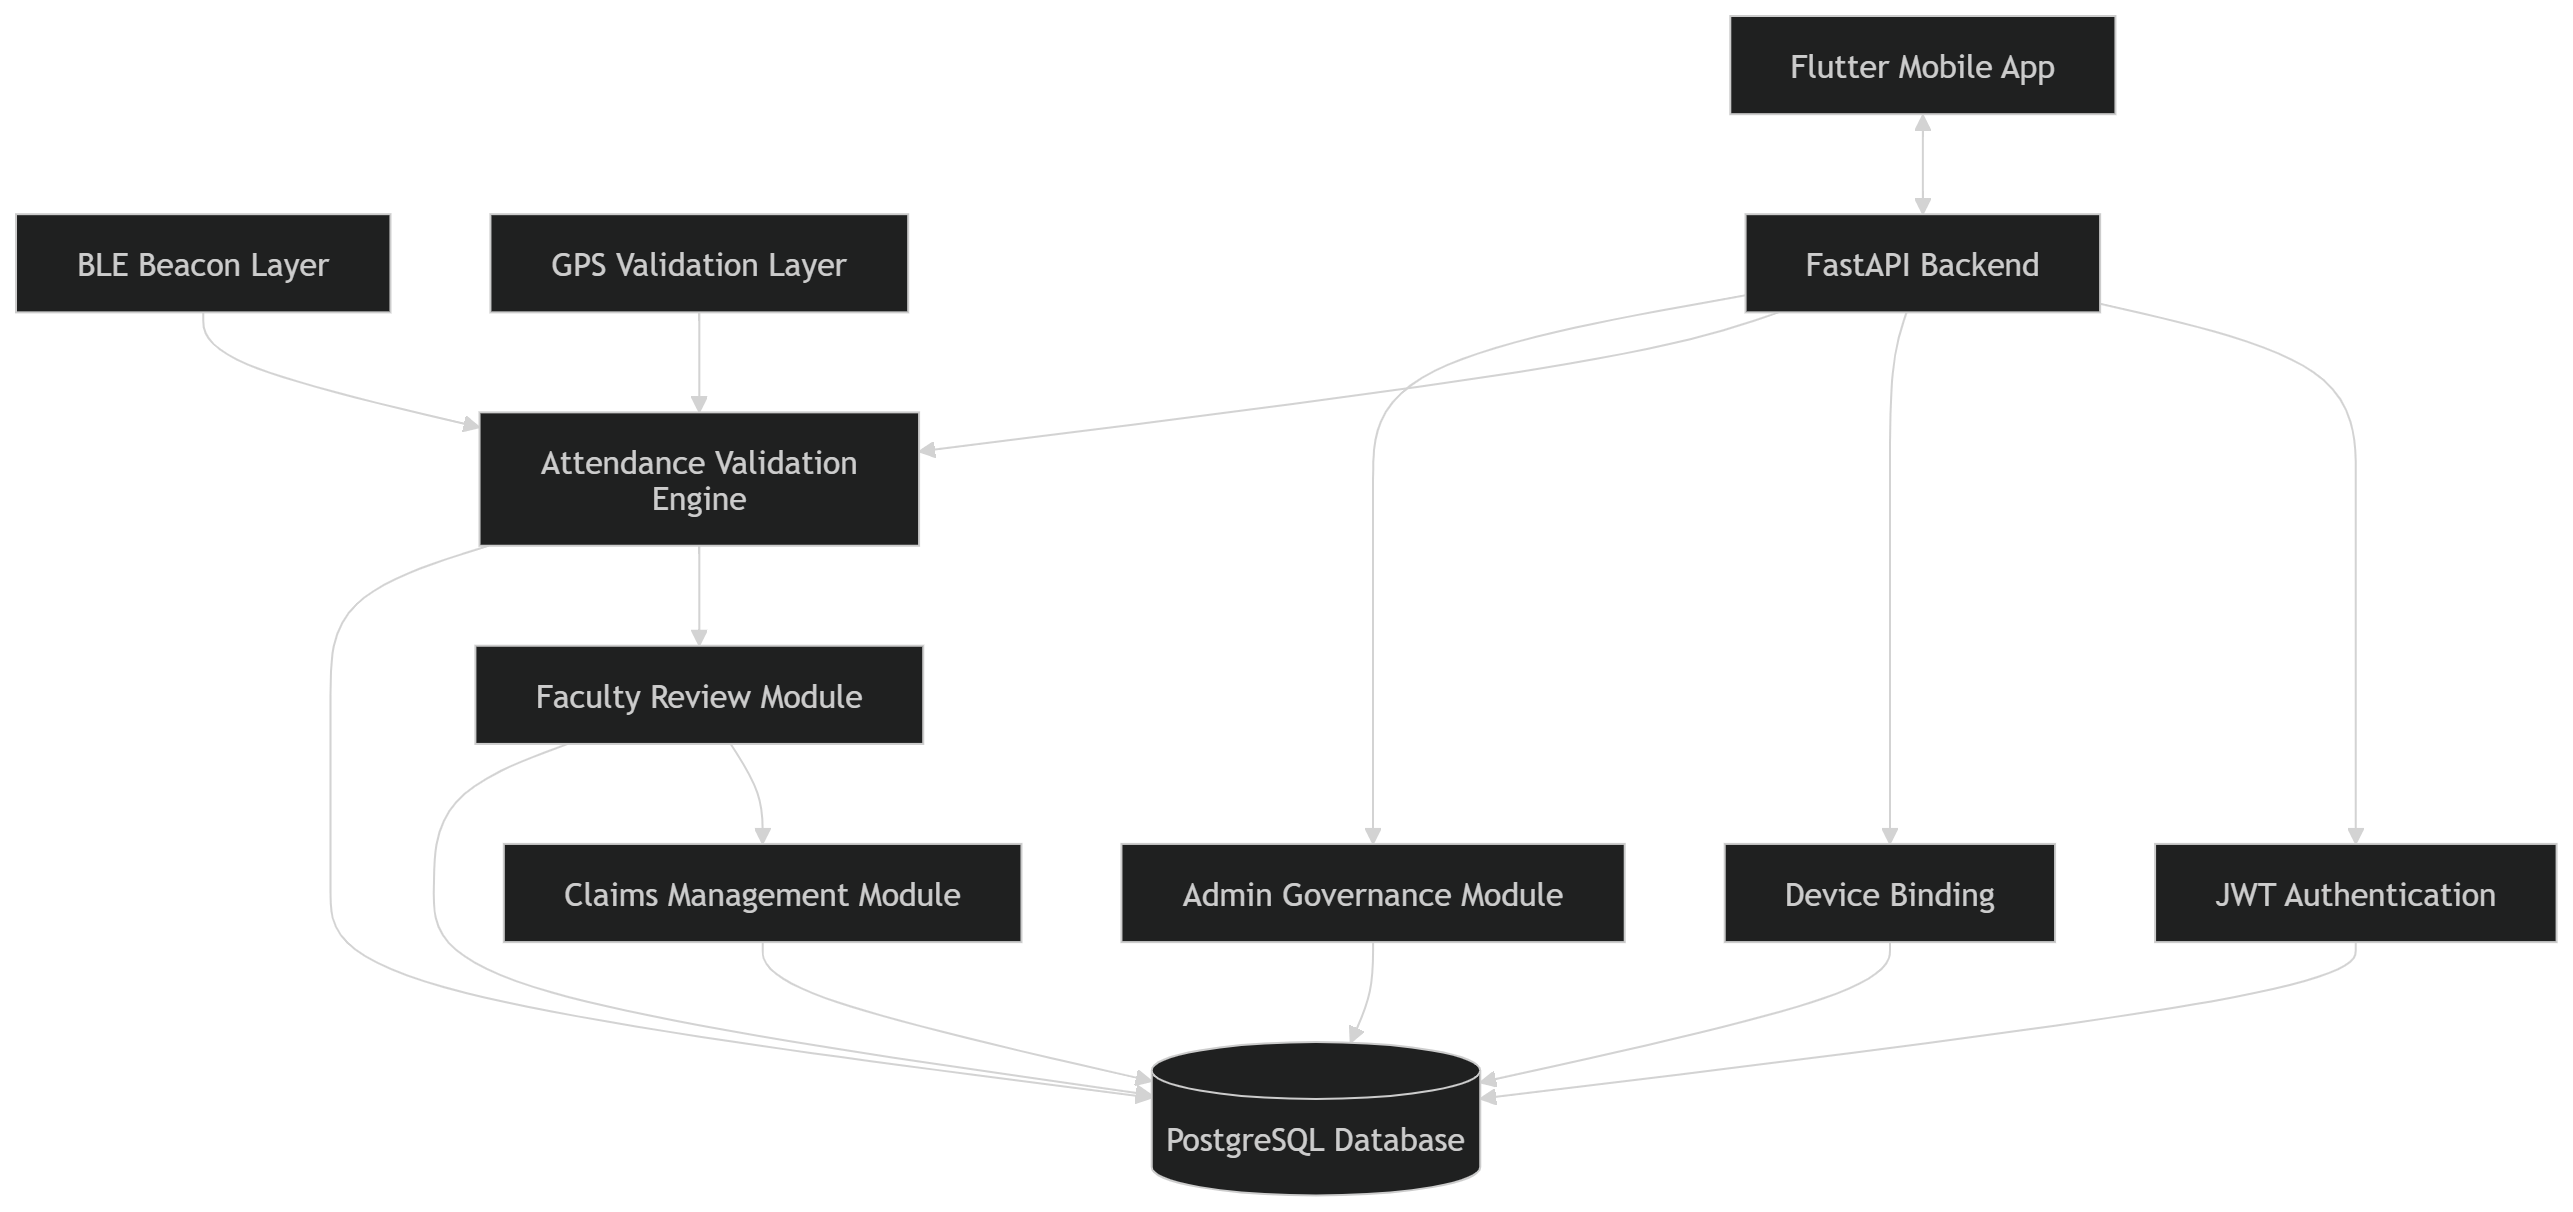
\includegraphics[width=\textwidth,height=0.72\textheight,keepaspectratio]{images/design/architecture/system_architecture.png}
    \caption{Layered Architecture Diagram}
    \label{fig:layered-architecture}
\end{figure}
% Image inserted: images/design/architecture/system_architecture.png (reused from Figure 3.1 -- no separate
% layered-architecture diagram was supplied; this is the closest available architecture asset).

\section{Technology Choices Revisited}

\begin{table}[htbp]
\centering
\caption{Implementation Technologies by Layer}
\label{tab:impl-tech}
\begin{tabularx}{\textwidth}{|l|X|}
\hline
\textbf{Layer} & \textbf{Technology} \\
\hline
Mobile Application & Flutter / Dart \\
\hline
Backend API & FastAPI (Python) \\
\hline
Database & PostgreSQL \\
\hline
ORM & SQLAlchemy \\
\hline
Migrations & Alembic \\
\hline
Authentication & JWT \\
\hline
BLE Infrastructure & ESP32 \\
\hline
Transport & REST over HTTPS \\
\hline
\end{tabularx}
\end{table}

\section{Evidence-Fusion Philosophy}

The architectural premise underlying the system is that attendance should not be decided on the strength of a single signal. Every submission is evaluated against two independent evidence sources -- BLE proximity and GPS location -- combined with a device-identity check, before a decision is reached. The attendance engine itself does not autonomously issue a final rejected outcome. Instead, it either confirms a submission when the collected evidence is sufficiently trustworthy, flags the submission for faculty review when the evidence is weak, inconsistent, or suspicious, or blocks the submission entirely when no BLE evidence is captured. This design keeps final rejection as a faculty governance action rather than an automatic system decision.

\section{Major Functional Modules}

The system is organised into six cooperating modules:

\begin{itemize}
    \item \textbf{Student Module} -- attendance submission and history.
    \item \textbf{Faculty Module} -- session governance and attendance review.
    \item \textbf{Admin Module} -- academic and infrastructure governance.
    \item \textbf{BLE Module} -- beacon discovery and proximity validation.
    \item \textbf{GPS Module} -- location capture and geofence validation.
    \item \textbf{Claims Module} -- dispute submission and resolution.
\end{itemize}

\section{Student Module}

The student-facing module supports login, discovery of active sessions scoped to the student's enrolments, evidence collection and attendance submission, viewing of attendance history, claim submission, and profile management. The attendance flow proceeds as: authenticate, discover an eligible session, collect BLE evidence, collect GPS evidence, submit, and receive an immediate system response. The automated outcome is either \textbf{CONFIRMED} or \textbf{FLAGGED for faculty review}. If the submission fails a mandatory precondition --- such as missing BLE evidence, invalid session state, duplicate submission, stale or replayed BLE payload, or device-binding failure --- the request is blocked and no attendance record is created.

\begin{figure}[htbp]
    \centering
    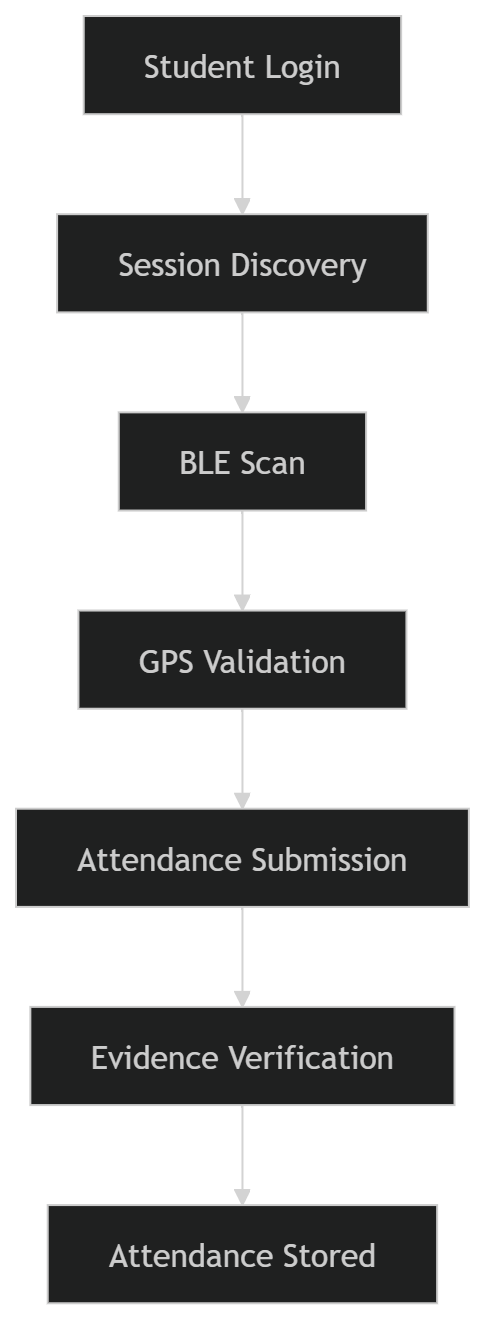
\includegraphics[width=\textwidth,height=0.72\textheight,keepaspectratio]{images/design/architecture/attendance_flow.png}
    \caption{Student Attendance Workflow}
    \label{fig:student-workflow}
\end{figure}
% Image inserted: images/design/architecture/attendance_flow.png

\section{Faculty Module}

Faculty members start and close attendance sessions, monitor submissions as they arrive, inspect the underlying BLE and GPS evidence for any flagged record, and confirm or reject those records with a recorded reason. A faculty dashboard surfaces active sessions, pending reviews, and pending claims at a glance.

\begin{figure}[htbp]
    \centering
    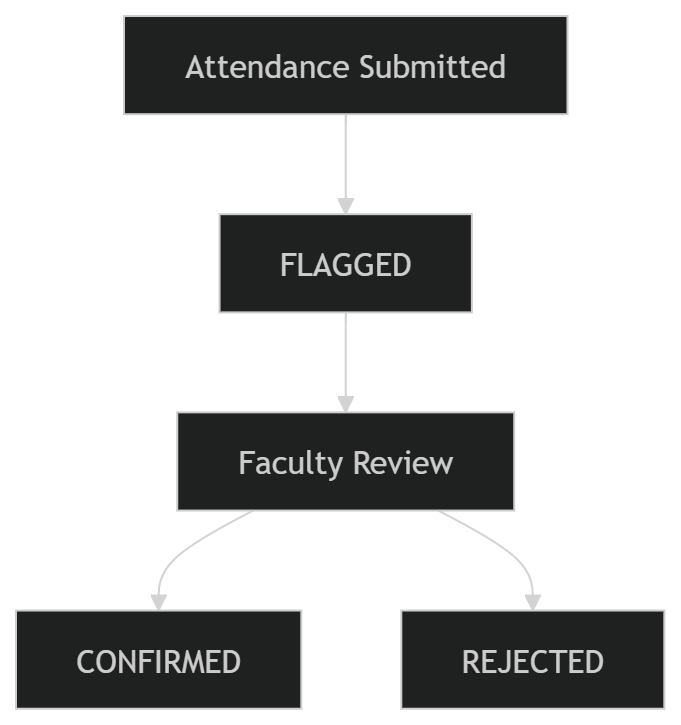
\includegraphics[width=\textwidth,height=0.72\textheight,keepaspectratio]{images/design/architecture/faculty_review_flow.png}
    \caption{Faculty Review Workflow}
    \label{fig:faculty-workflow}
\end{figure}
% Image inserted: images/design/architecture/faculty_review_flow.png

\section{Administrative Module}

Administrators manage the full academic hierarchy -- students, faculty, courses, faculty-course assignments, enrolments, classrooms -- together with the trusted-beacon registry and device-binding lifecycle (including unbinding a device when a student loses or replaces their phone).

\begin{figure}[htbp]
    \centering
    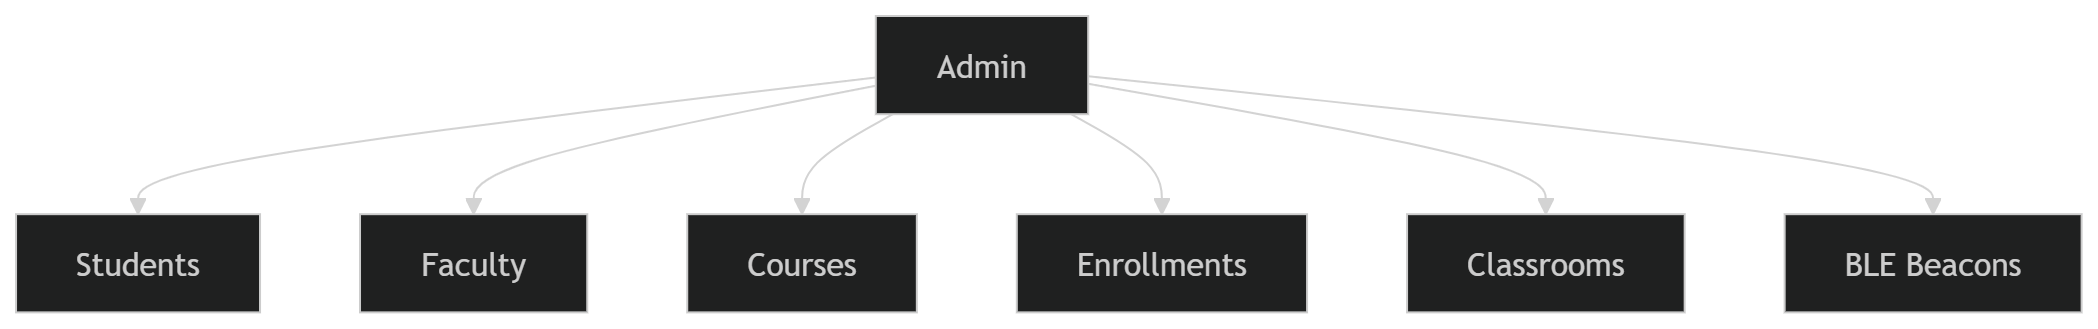
\includegraphics[width=\textwidth,height=0.72\textheight,keepaspectratio]{images/design/architecture/admin_governance_flow.png}
    \caption{Admin Governance Workflow}
    \label{fig:admin-workflow}
\end{figure}
% Image inserted: images/design/architecture/admin_governance_flow.png

\section{BLE Module}

Each classroom beacon, built on an ESP32 microcontroller, periodically broadcasts a small payload containing a beacon identifier, a freshly generated nonce, a timestamp, and an HMAC signature computed over the payload using a secret known only to the backend and that specific beacon. The mobile application scans for and reads this payload, and the backend independently recomputes the signature to confirm the broadcast is genuine before accepting it as evidence.

\textit{Example BLE Beacon Payload:}

\begin{lstlisting}
{
  "beacon_id": "ESP32-A1",
  "nonce": "xyz123",
  "timestamp": 1750000000,
  "signature": "..."
}
\end{lstlisting}

\section{GPS Module}

The mobile application captures the device's latitude, longitude, and reported accuracy at the moment of submission. The backend computes the distance between the reported coordinates and the classroom's registered location and checks that distance against the classroom's configured geofence radius, producing one of three outcomes: inside the geofence, outside the geofence, or accuracy too low to evaluate reliably.

\section{Evidence-Fusion Decision Table}

\begin{table}[htbp]
\centering
\caption{Attendance Decision Matrix}
\label{tab:decision-matrix}
\begin{tabularx}{\textwidth}{|l|l|X|}
\hline
\textbf{BLE Result} & \textbf{GPS Result} & \textbf{Decision} \\
\hline
Valid & Valid & CONFIRMED \\
\hline
Valid & Invalid / Outside Geofence / Low Accuracy & FLAGGED for faculty review \\
\hline
Invalid / Weak / Suspicious & Valid & FLAGGED for faculty review \\
\hline
Invalid / Weak / Suspicious & Invalid / Outside Geofence / Low Accuracy & FLAGGED for faculty review \\
\hline
No BLE evidence captured & Any GPS result & Submission blocked; no attendance record is created \\
\hline
\end{tabularx}
\end{table}

The matrix in Table~\ref{tab:decision-matrix} represents the automated outcome produced by the attendance engine only. A record marked as FLAGGED is not rejected automatically; instead, it is routed to the responsible faculty member for evidence-based review. If no BLE evidence is captured, the submission is blocked and no attendance record is created. Final rejection, where applicable, is therefore a faculty governance decision rather than an automatic system outcome.

\begin{figure}[htbp]
    \centering
    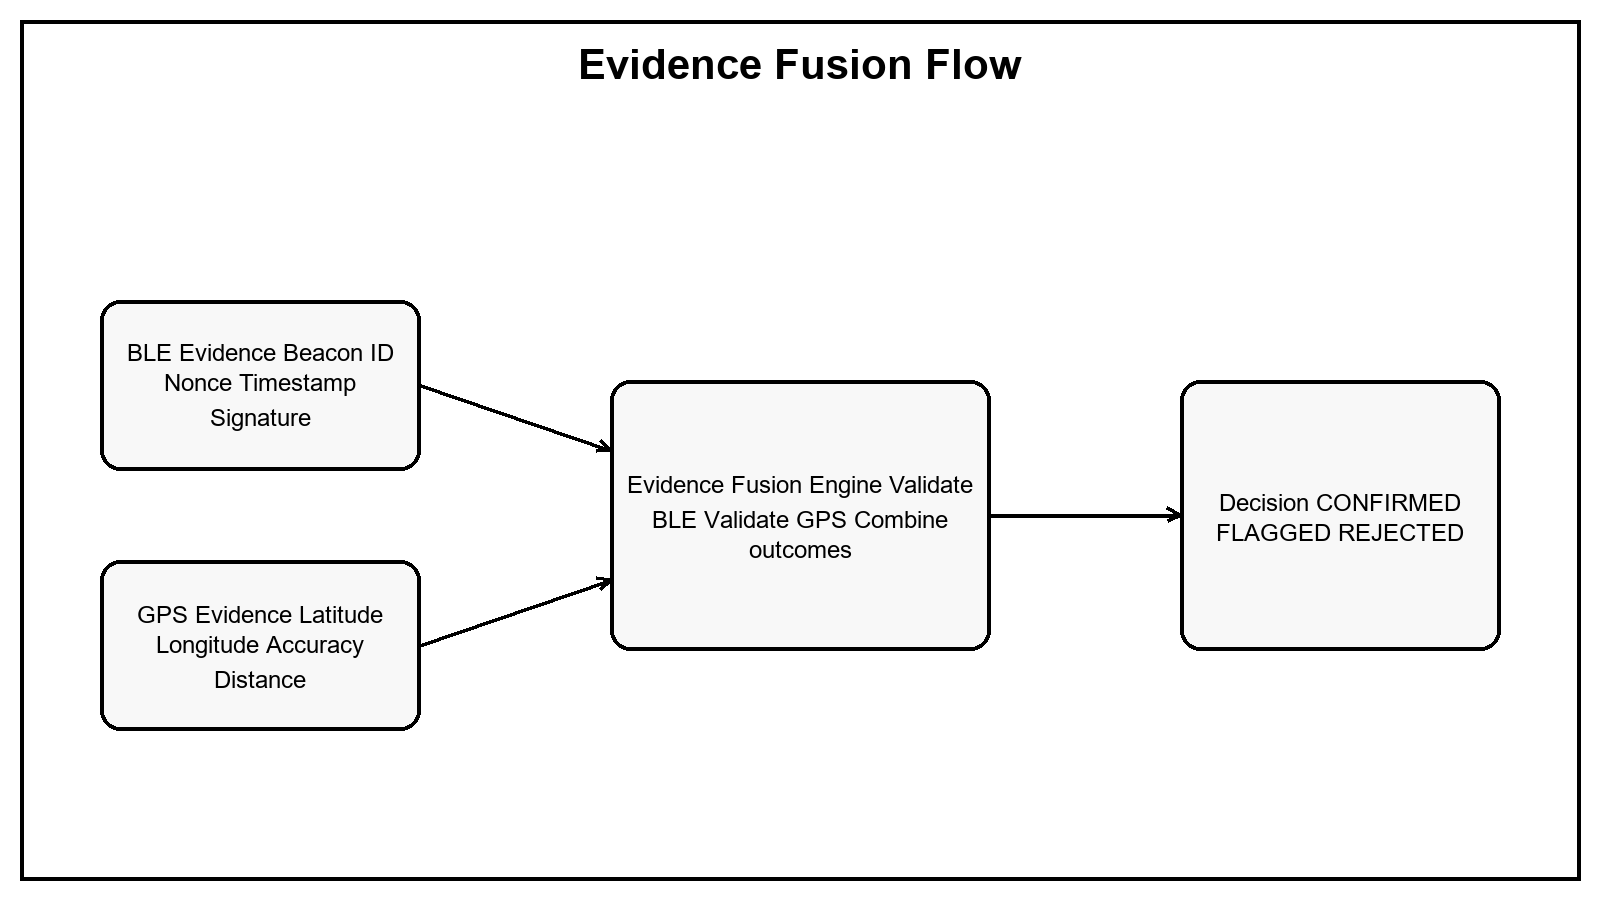
\includegraphics[width=\textwidth,height=0.72\textheight,keepaspectratio]{images/fig4_5_evidence_fusion.png}
    \caption{Evidence Fusion Flow}
    \label{fig:evidence-fusion}
\end{figure}

\section{Sequence Diagram: Attendance Submission}

Figure~\ref{fig:sequence-submission} traces a single attendance submission as a sequence of messages between the student, the Flutter client, the backend API, the BLE and GPS validators, the decision engine, and the database. This view makes explicit the order in which evidence is collected and validated, and clarifies that the decision engine only acts once both evidence channels have returned a result.

\begin{figure}[htbp]
    \centering
    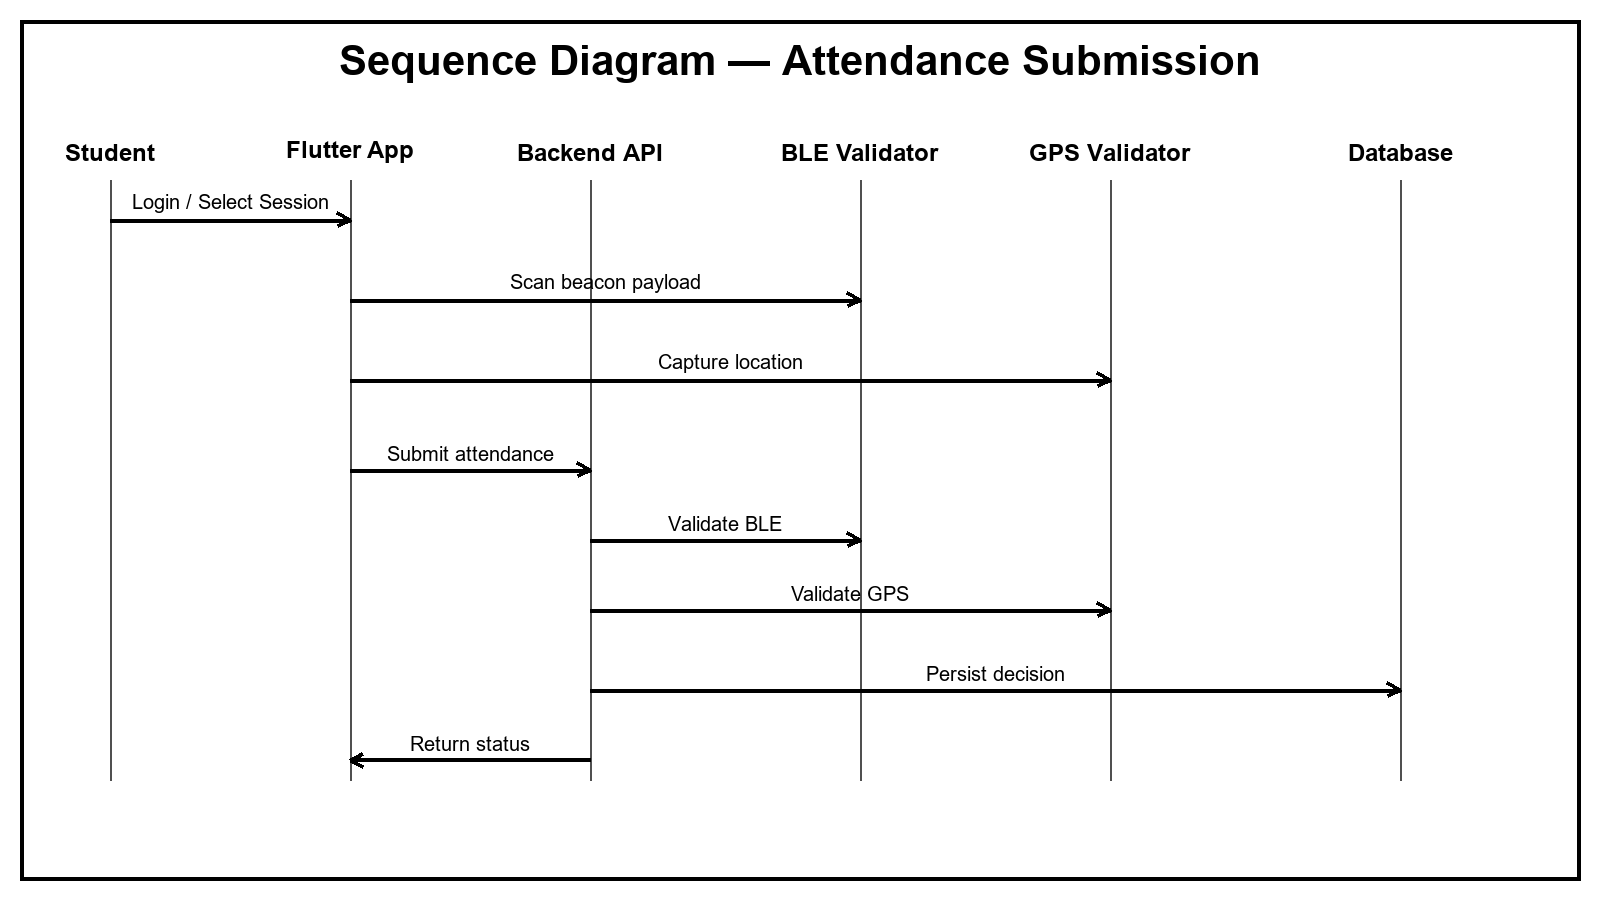
\includegraphics[width=\textwidth,height=0.72\textheight,keepaspectratio]{images/fig4_7_sequence_diagram.png}
    \caption{Sequence Diagram -- Attendance Submission}
    \label{fig:sequence-submission}
\end{figure}

\section{Security Architecture}
\label{sec:security-architecture}

To make the security reasoning behind the layered architecture of Section~4.3 explicit, Figure~\ref{fig:security-architecture} traces a single request as it passes through every security checkpoint between the student's device and the persisted record, restated below as a checkpoint pipeline.

\begin{lstlisting}
Student Device
      |
      v
JWT Authentication (identity + role)
      |
      v
Backend API (FastAPI)
      |
      v
BLE Validation (nonce, freshness, HMAC signature)
      |
      v
GPS Validation (geofence distance, accuracy)
      |
      v
Evidence Fusion / Decision Engine
      |
      v
Faculty Review (for FLAGGED records)
      |
      v
PostgreSQL Database (persisted record)
      |
      v
Audit Log (append-only)
\end{lstlisting}

\begin{figure}[htbp]
    \centering
    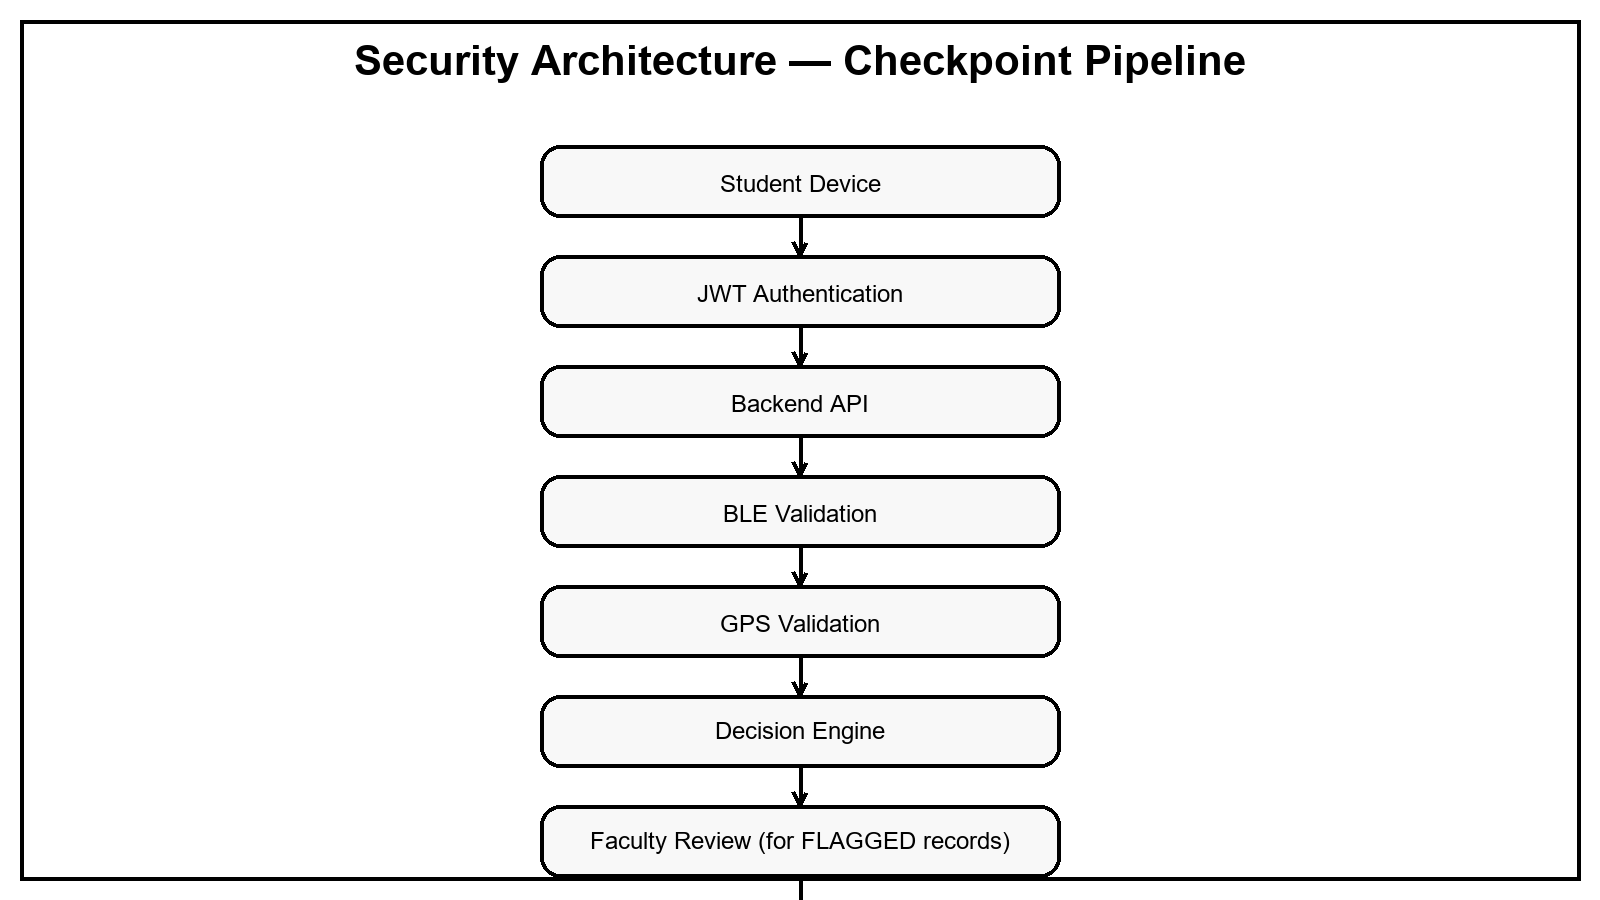
\includegraphics[width=\textwidth,height=0.72\textheight,keepaspectratio]{images/fig4_9_security_architecture.png}
    \caption{Security Architecture -- Checkpoint Pipeline}
    \label{fig:security-architecture}
\end{figure}

Each checkpoint in this pipeline is independently capable of rejecting a request, so that no single compromised layer is sufficient to produce an unwarranted CONFIRMED outcome; this is the architectural counterpart of the threat model presented in Table~\ref{tab:threat-model}.

\section{Data Flow Diagram (Level 0)}
\label{sec:dfd}

Figure~\ref{fig:dfd-level0} presents a context-level (Level~0) data-flow diagram for the system, showing the three external actors -- Student, Faculty, and Administrator -- and their principal data exchanges with the HKS ATTENDANCE platform as a single process.

\begin{figure}[htbp]
    \centering
    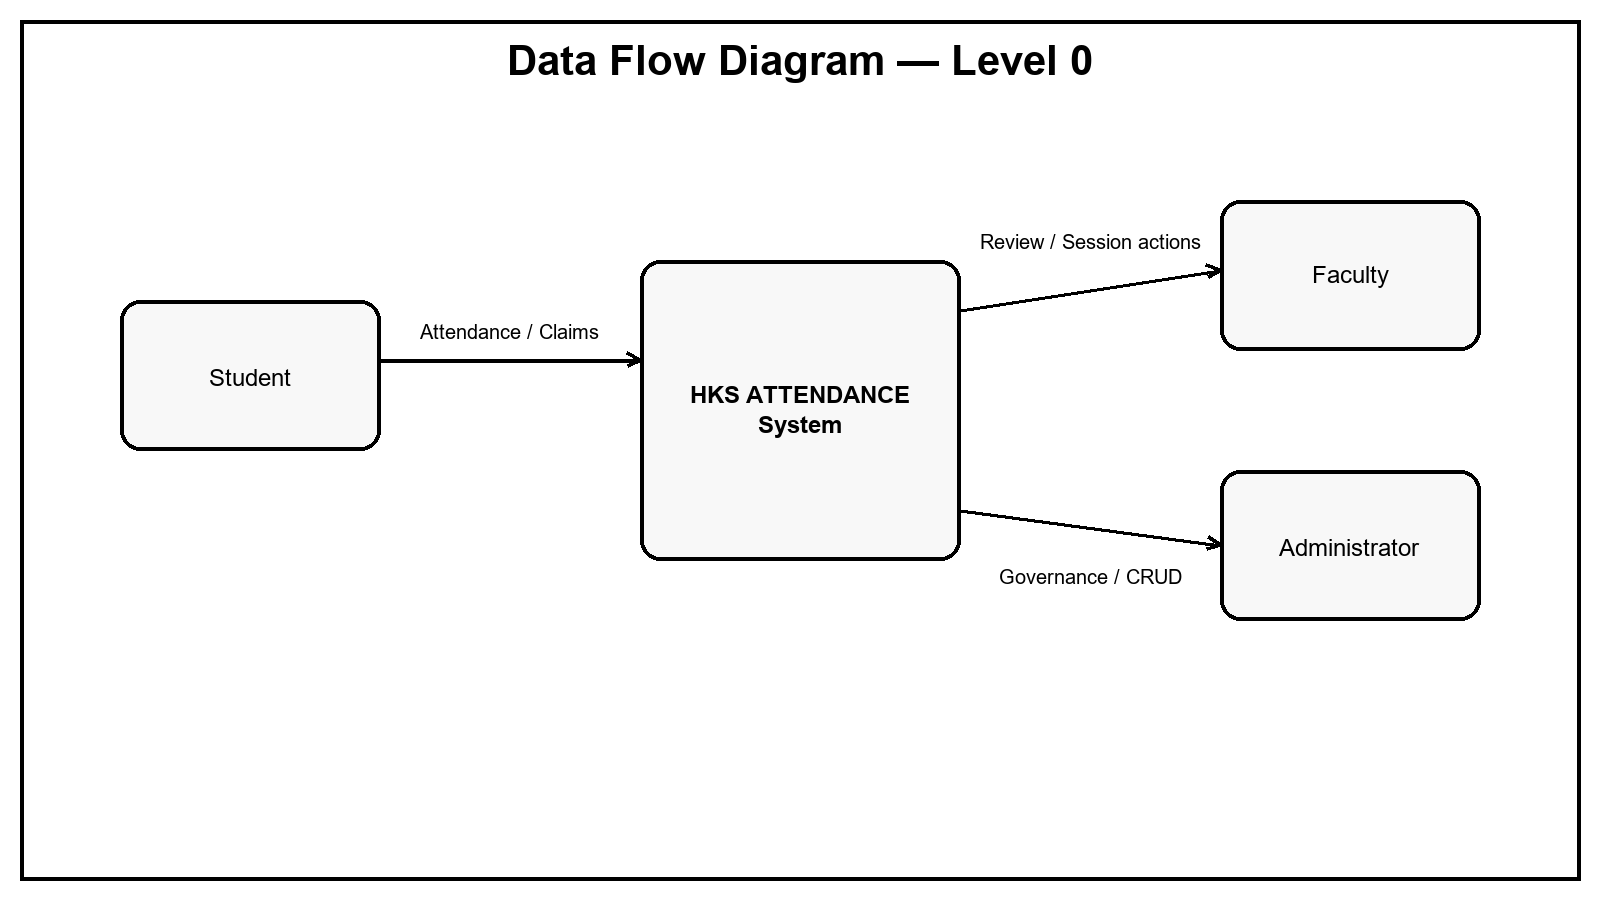
\includegraphics[width=\textwidth,height=0.72\textheight,keepaspectratio]{images/fig4_10_dfd_level0.png}
    \caption{Data Flow Diagram -- Level 0 (Context Diagram)}
    \label{fig:dfd-level0}
\end{figure}
% TODO: insert the Level-0 DFD at images/fig4_10_dfd_level0.png
% ASSUMPTION: no supplied image asset corresponds specifically to this diagram; left pending.

\section{Component and Package Diagrams}
\label{sec:component-package}

Figure~\ref{fig:component-diagram} shows the major software components within the backend (routers, services, security, and data-access layers) and their dependencies, while Figure~\ref{fig:package-diagram} shows the corresponding package-level organisation of the Flutter mobile client described in Section~6.3.

\begin{figure}[htbp]
    \centering
    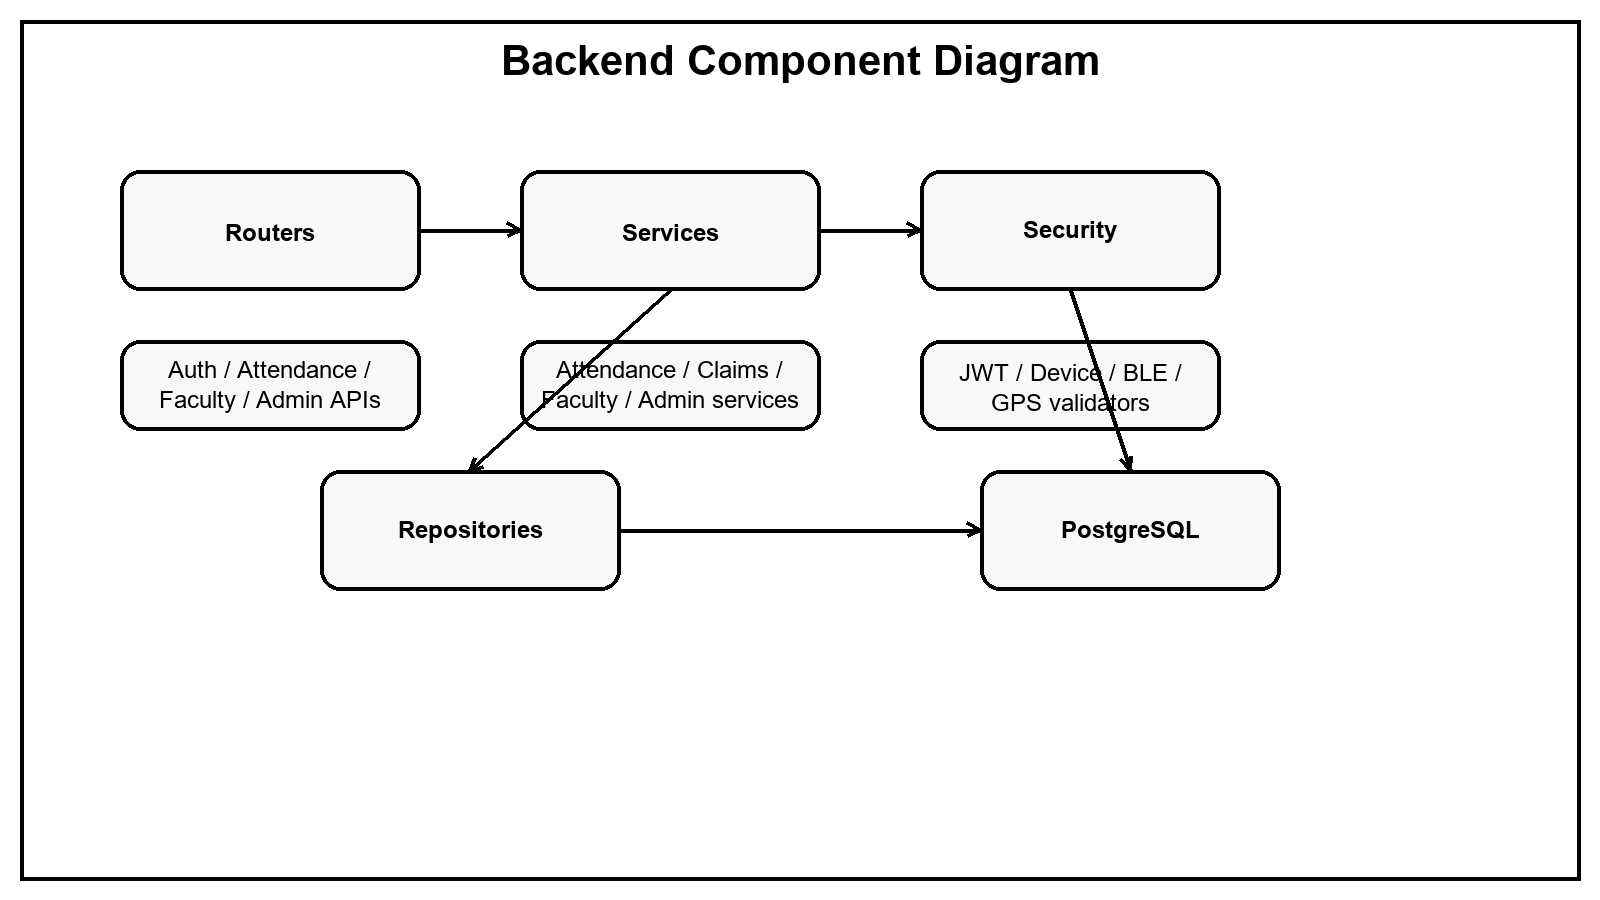
\includegraphics[width=\textwidth,height=0.72\textheight,keepaspectratio]{images/fig4_11_component_diagram.png}
    \caption{Backend Component Diagram}
    \label{fig:component-diagram}
\end{figure}
% TODO: insert the backend component diagram at images/fig4_11_component_diagram.png
% ASSUMPTION: no supplied image asset corresponds specifically to this diagram; left pending.

\begin{figure}[htbp]
    \centering
    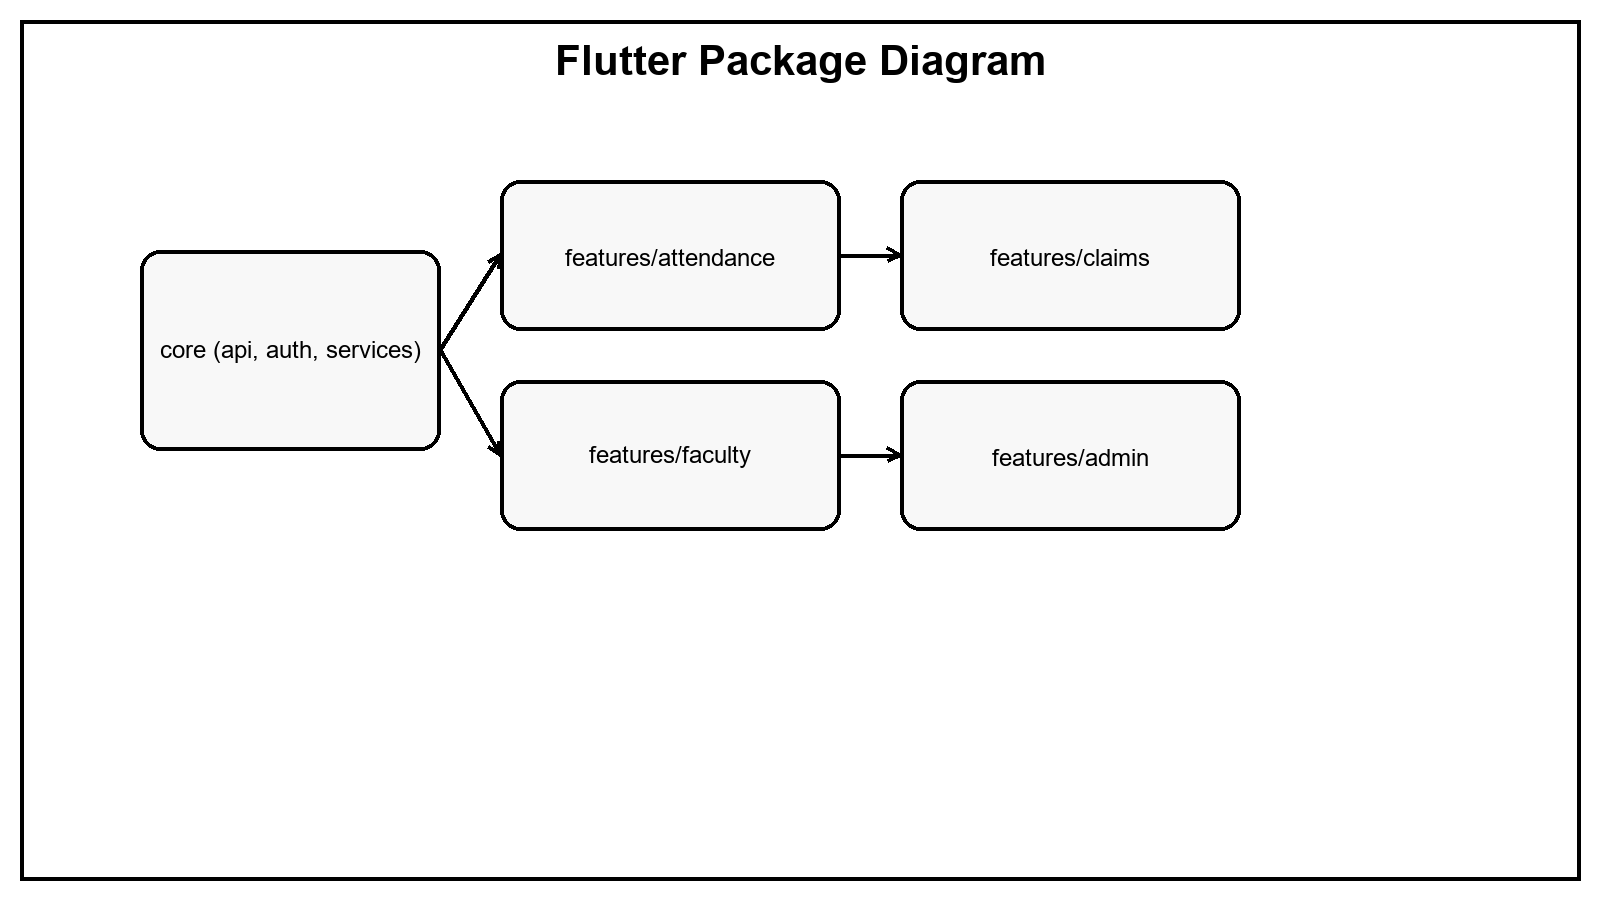
\includegraphics[width=\textwidth,height=0.72\textheight,keepaspectratio]{images/fig4_12_package_diagram.png}
    \caption{Mobile Application Package Diagram}
    \label{fig:package-diagram}
\end{figure}
% TODO: insert the mobile application package diagram at images/fig4_12_package_diagram.png
% ASSUMPTION: no supplied image asset corresponds specifically to this diagram; left pending.

\section{Authentication Design}

Login credentials are validated against the stored, hashed password, and a JWT access token is issued on success. The token is attached to all subsequent requests and is required for attendance submission, claims, and any faculty or administrative action.

\section{Device-Binding Design}

A student's first successful login registers the device they are using as their bound device. Subsequent attendance submissions are checked against this binding; a request originating from an unrecognised device is rejected outright. Should a student need to switch devices, an administrator must first unbind the old device, after which the student's next successful login registers the replacement.

\section{Claims Module Design}

Only attendance records in the REJECTED state may be claimed, and only one claim may be opened per attendance record. A submitted claim moves through PENDING, and is resolved by the faculty member who owns the relevant course into either APPROVED -- which moves the underlying attendance record to CONFIRMED -- or REJECTED, which leaves the original outcome unchanged. Every resolution is written to the audit log.

\begin{figure}[htbp]
    \centering
    
\includegraphics[width=0.85\textwidth]{images/design/architecture/claims_flow.png}
    \caption{Claims Resolution Workflow}
    \label{fig:claims-workflow}
\end{figure}
% Image inserted: images/design/architecture/claims_flow.png

\section{Audit-Logging Design}

Every governance-relevant action -- confirming or rejecting attendance, approving or rejecting a claim, unbinding a device, closing a session -- produces a permanent log entry recording the actor, the action, the before-and-after state, and a timestamp.

\section{Session-Lifecycle Design}

Attendance sessions move through three states: ACTIVE, CLOSED (closed manually by faculty), and EXPIRED (closed automatically once the configured duration elapses). Attendance may only be submitted while a session is ACTIVE.

\section{Attendance Status State Diagram}

Independently of session lifecycle, each individual attendance attempt carries its own status, which moves through a small set of well-defined states from creation to final resolution, including the claims path for records that are initially rejected. Figure~\ref{fig:status-state} shows this state diagram.

\begin{figure}[htbp]
    \centering
    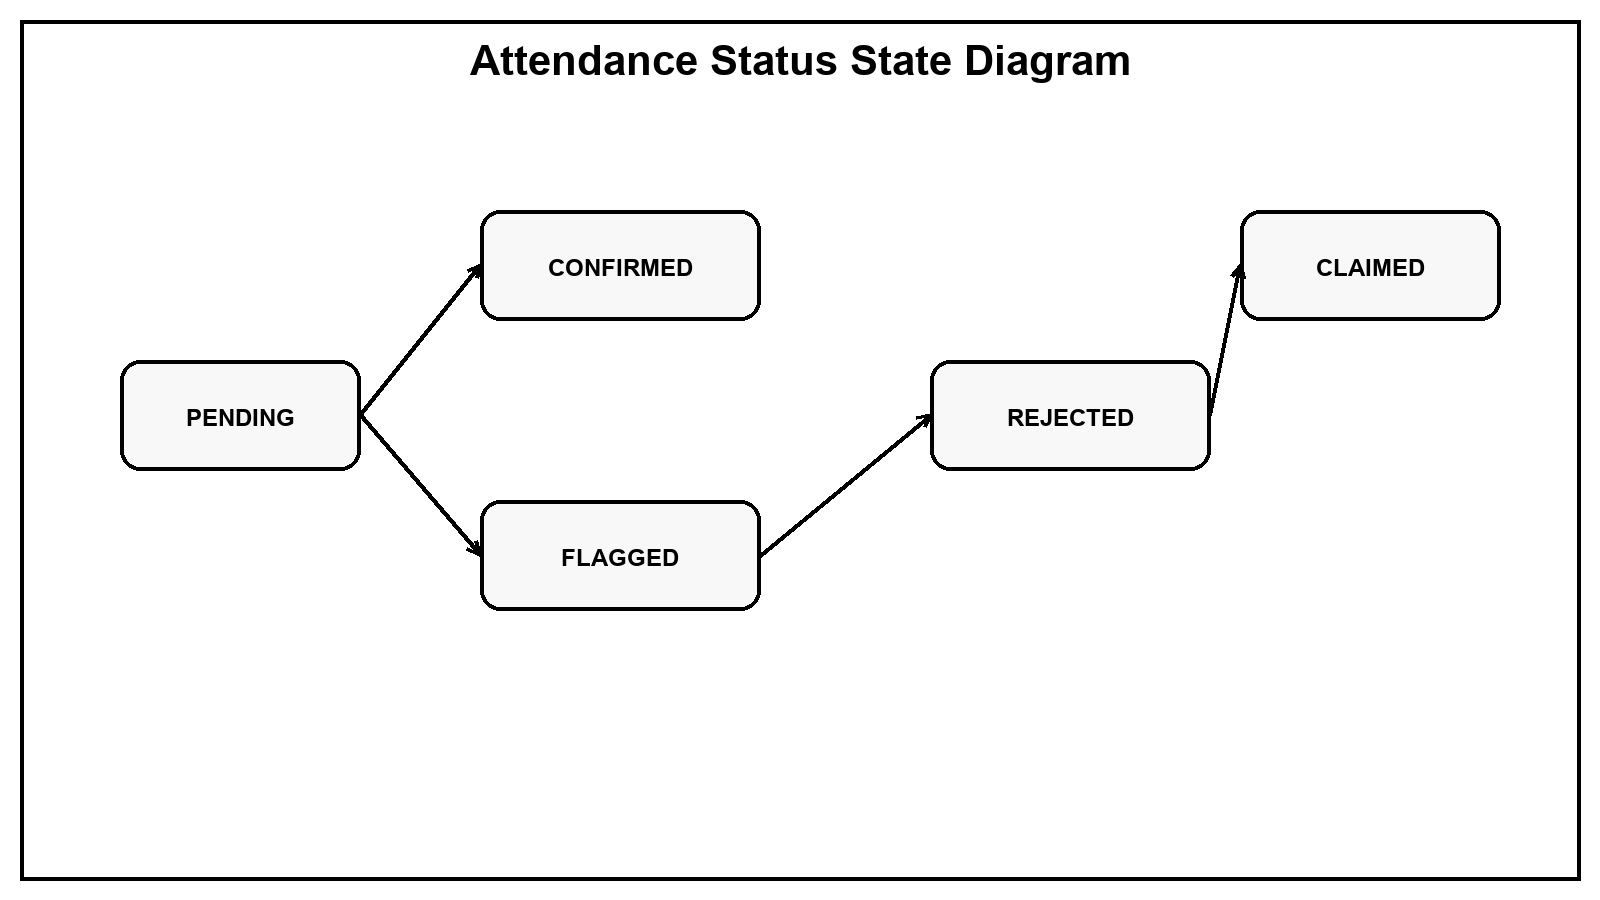
\includegraphics[width=0.85\textwidth]{images/fig4_8_status_state.png}
    \caption{Attendance Status State Diagram}
    \label{fig:status-state}
\end{figure}
% TODO: insert the attendance status state diagram at images/fig4_8_status_state.png
% ASSUMPTION: no supplied image asset corresponds specifically to this diagram; left pending.

\section{Use-Case Summary}

\begin{table}[htbp]
\centering
\caption{Representative Use Cases by Role}
\label{tab:use-cases}
\begin{tabularx}{\textwidth}{|l|X|}
\hline
\textbf{Role} & \textbf{Representative Use Cases} \\
\hline
Student & Login; discover sessions; submit attendance; view history; submit claims \\
\hline
Faculty & Start/close sessions; review attendance; resolve claims \\
\hline
Administrator & Manage users, courses, enrolments, classrooms, beacons, and devices \\
\hline
\end{tabularx}
\end{table}

\section{Design Advantages}
\begin{itemize}
    \item \textbf{Security}: decisions rest on multiple independent validation layers.
    \item \textbf{Governance}: faculty and administrators retain meaningful oversight.
    \item \textbf{Auditability}: every consequential action is logged.
    \item \textbf{Modularity}: the six functional modules can evolve largely independently.
    \item \textbf{Extensibility}: the architecture leaves room for additional evidence sources in the future.
\end{itemize}

\section{Chapter Summary}

This chapter presented the layered architecture, the major functional modules, the evidence-fusion logic, the security-checkpoint pipeline, and the context-, component-, and package-level diagrams at the heart of HKS ATTENDANCE. The next chapter describes the database design that underpins this architecture.

% =============================================================================
% CHAPTER 5: DATABASE DESIGN
% =============================================================================
\chapter{Database Design}
\label{chap:database}

\section{Introduction}

Every attendance decision, governance action, and dispute resolution in HKS ATTENDANCE ultimately rests on data persisted in PostgreSQL. This chapter describes the relational schema underpinning the platform, the reasoning behind its major entities, and the integrity constraints that keep the academic and security records consistent. PostgreSQL was chosen for its ACID guarantees, mature support for foreign-key enforcement, and proven reliability under the kind of transactional load an attendance system generates.

\section{Design Objectives}
\begin{itemize}
    \item Preserve attendance records as immutable, accurate history once written.
    \item Support faculty review and administrative governance directly through the schema.
    \item Store BLE evidence, GPS evidence, device bindings, and audit entries durably.
    \item Scale comfortably as the number of students, courses, sessions, and historical records grows.
    \item Preserve enough history to support after-the-fact dispute investigation.
\end{itemize}

\section{Database Design Philosophy}

Before describing individual tables, it is useful to state the design principles applied consistently across the schema:

\begin{itemize}
    \item \textbf{Normalisation} -- the schema is normalised to third normal form (Section~5.4), so that each fact is stored exactly once and update anomalies are avoided.
    \item \textbf{Primary keys} -- every table is keyed by a surrogate integer or UUID primary key, kept independent of any business attribute that might change over time.
    \item \textbf{Foreign keys} -- every cross-table reference (a session referencing a course, an attempt referencing a session, and so on) is enforced as a foreign-key constraint at the database level, not merely checked in application code.
    \item \textbf{Indexes} -- foreign-key columns and columns used in frequent lookups (for example, a student's active sessions, or a beacon's nonce history) are indexed to keep query latency low as the volume of historical data grows.
    \item \textbf{Constraints} -- uniqueness constraints (for example, one device per student, one open claim per attendance attempt) are enforced in the schema itself, so that the invariant holds even if application-level validation is bypassed or contains a bug.
    \item \textbf{Transactions} -- multi-step writes (for example, approving a claim and updating the underlying attendance record) are wrapped in a single database transaction, so that a failure partway through cannot leave the two records in an inconsistent state.
    \item \textbf{Referential integrity} -- the database, not the application, is the final authority on whether a reference between two rows is valid; this is treated as a security boundary as much as a correctness one (Section~5.9).
\end{itemize}

\section{Normalisation Approach}

The schema was normalised to third normal form. Atomic fields (for example, separate first- and last-name columns rather than a single combined name field) satisfy first normal form; every non-key attribute depends on the whole of its table's primary key, satisfying second normal form; and course information is stored once in a Courses table rather than repeated on every attendance record, satisfying third normal form and avoiding the update anomalies that denormalised duplication would otherwise introduce.

\section{Entity Overview}

The principal entities are Users, Devices, Courses, FacultyCourses, Enrollments, Classrooms, TrustedBLEBeacons, BeaconSecrets, AttendanceSessions, AttendanceAttempts, AttendanceBLEEvidence, AttendanceGPSEvidence, AttendanceClaims, and FacultyActionLogs, supported by an AuthSessions table for token lifecycle tracking and a BLENonceCache table dedicated to replay protection.

\section{Key Tables}

\subsection{Users}

\begin{table}[htbp]
\centering
\caption{Users Table}
\label{tab:users-table}
\begin{tabularx}{\textwidth}{|l|X|}
\hline
\textbf{Field} & \textbf{Description} \\
\hline
id & Primary key \\
\hline
full\_name & Full name of the user \\
\hline
email & Unique login identifier \\
\hline
password\_hash & Securely hashed password -- never stored in plain text \\
\hline
role & STUDENT / FACULTY / ADMIN \\
\hline
is\_active & Account status flag \\
\hline
created\_at & Account creation timestamp \\
\hline
\end{tabularx}
\end{table}

\subsection{Devices}
Captures the binding between a student account and the single device authorised to submit attendance on its behalf, storing a unique device identifier and the timestamp at which the binding was created.

\subsection{Courses, FacultyCourses, and Enrollments}
Courses store the academic catalogue; FacultyCourses establishes which faculty member owns a given course; Enrollments establishes which students are eligible to attend sessions for that course. This three-table structure replaced an earlier design in which faculty were tied directly to classrooms rather than courses -- a model abandoned once it became clear that faculty regularly teach the same course in different rooms across a term.

\subsection{Classrooms}
Stores the physical reference point -- name, latitude, longitude, and geofence radius -- against which GPS evidence is validated. Classrooms are not owned by any single faculty member, since the same room is typically shared across multiple courses and instructors.

\subsection{TrustedBLEBeacons and BeaconSecrets}
TrustedBLEBeacons records which beacon identifiers are recognised as legitimate for a given classroom, while BeaconSecrets stores the cryptographic key used to validate each beacon's HMAC signature -- kept in a separate table so that secret material can be rotated or audited independently of the beacon's operational metadata.

\subsection{AttendanceSessions}
Represents a single attendance window, tying together a faculty member, a course, a classroom, a status (ACTIVE / CLOSED / EXPIRED), a start time, and an expiry time.

\subsection{AttendanceAttempts}

\begin{table}[htbp]
\centering
\caption{AttendanceAttempts Table}
\label{tab:attendance-attempts}
\begin{tabularx}{\textwidth}{|l|X|}
\hline
\textbf{Field} & \textbf{Description} \\
\hline
id & Primary key \\
\hline
session\_id & Foreign key to AttendanceSessions \\
\hline
student\_id & Foreign key to Users \\
\hline
status & CONFIRMED / FLAGGED / REJECTED \\
\hline
submitted\_at & Submission timestamp \\
\hline
reviewed\_by & Faculty member who reviewed the record, if any \\
\hline
reviewed\_at & Review timestamp \\
\hline
resolution\_reason & Faculty-supplied explanation for the decision \\
\hline
\end{tabularx}
\end{table}

\subsection{AttendanceBLEEvidence and AttendanceGPSEvidence}
These two tables store, respectively, the beacon identifier, signal strength, sample count, nonce, signature, and client/server timestamps captured during BLE evidence collection; and the latitude, longitude, accuracy, computed distance from the classroom, and validation outcome captured during GPS evidence collection. Keeping the two evidence types in separate tables, both linked back to a single AttendanceAttempts row, allows faculty to inspect either channel independently during review.

\subsection{AttendanceClaims}
Stores the student's reason for disputing a rejected attendance record, the claim's current status (PENDING / APPROVED / REJECTED), and, once resolved, the identity of the resolving faculty member, the resolution timestamp, and the stated reason.

\subsection{FacultyActionLogs}
Records every governance decision taken by a faculty member -- confirming or rejecting attendance, approving or rejecting a claim -- together with the state before and after the action, for permanent audit purposes.

\section{Entity-Relationship Summary}

The dependency chain that ties the schema together runs: Users enrol into Courses; Faculty own Courses through FacultyCourses; Courses host AttendanceSessions in particular Classrooms; AttendanceSessions produce AttendanceAttempts; each AttendanceAttempt may carry BLE Evidence, GPS Evidence, and at most one Claim; and every Faculty decision against an attempt is mirrored into the FacultyActionLogs table. Figure~\ref{fig:er-diagram} shows this chain graphically; the principal relationships are walked through individually below.

\begin{figure}[htbp]
    \centering
    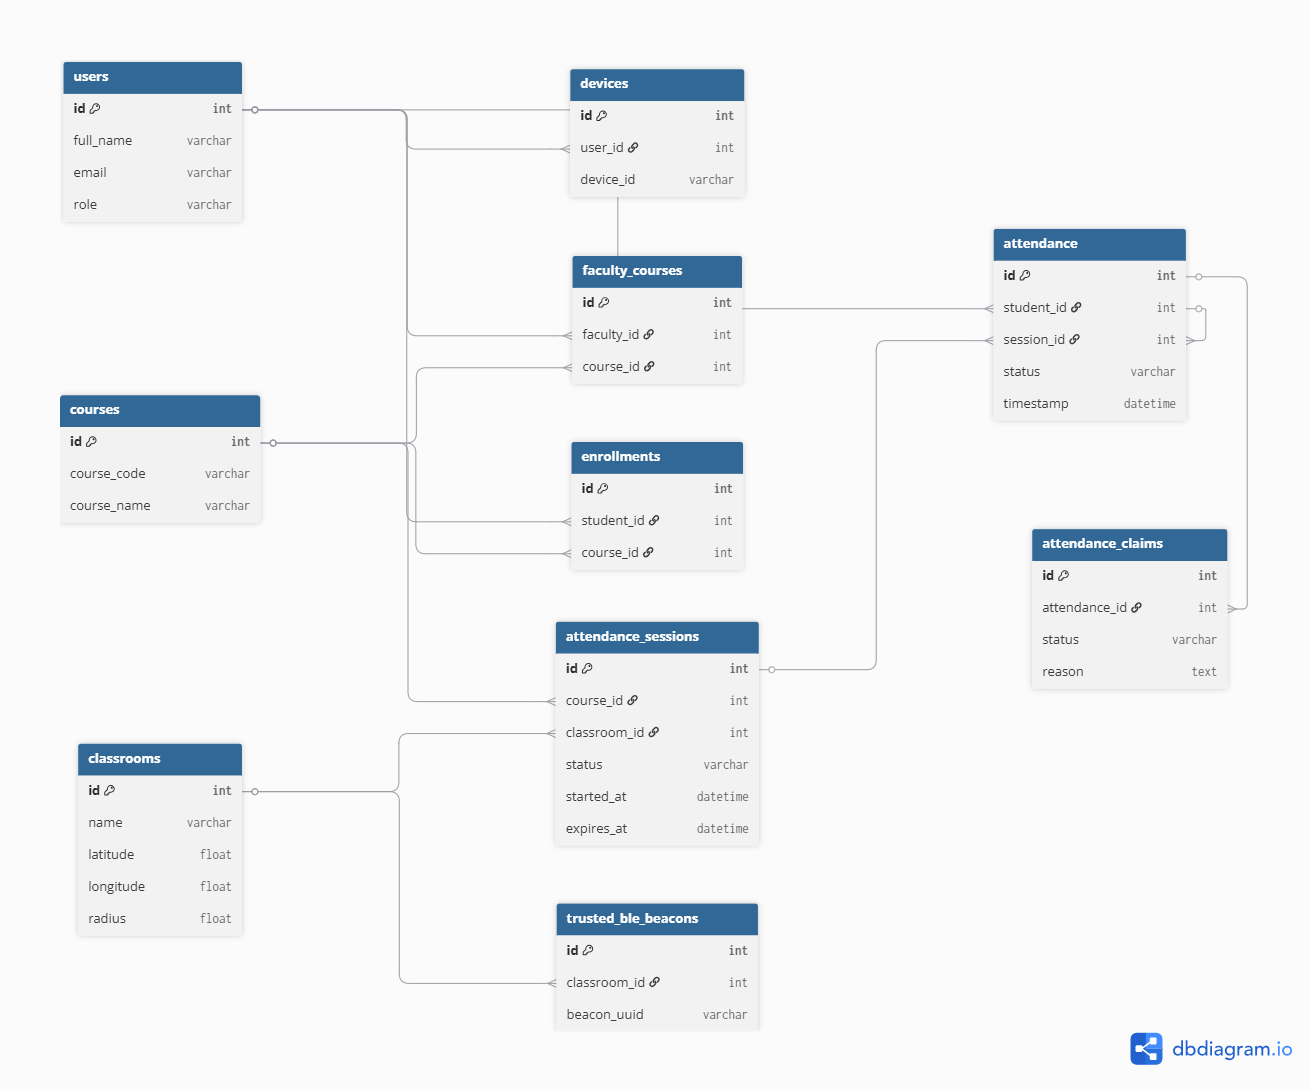
\includegraphics[width=0.85\textwidth]{images/design/er_diagram/attendance_er_diagram.png}
    \caption{Entity-Relationship Diagram}
    \label{fig:er-diagram}
\end{figure}
% Image inserted: images/design/er_diagram/attendance_er_diagram.png
\textit{Diagram constructed from the entity relationships enumerated in this section.}

\noindent\textbf{Users $\rightarrow$ Enrollments $\rightarrow$ Courses.} A student's eligibility to attend a session is never inferred informally; it is established by an explicit Enrollment row linking that student's Users record to a Courses record. This indirection is what allows the session-discovery logic described in Chapter~6 to be expressed as a single join rather than a special case.

\noindent\textbf{Courses $\rightarrow$ FacultyCourses $\rightarrow$ Users.} Course ownership is similarly explicit: a FacultyCourses row links a Courses record to the Users record of the faculty member responsible for it, which is what the session-ownership checks described in Chapter~4 rely on to prevent one instructor from acting on another's session.

\noindent\textbf{Courses / Classrooms $\rightarrow$ AttendanceSessions.} An AttendanceSessions row cannot exist without a valid course and a valid classroom; this is what allows the system to know, for any active session, both which geofence to validate GPS evidence against and which students are eligible to submit to it.

\noindent\textbf{AttendanceSessions $\rightarrow$ AttendanceAttempts.} Each attendance submission is recorded as a row in AttendanceAttempts that references the session it was submitted against, allowing the same student to have independent, separately auditable attempts across different sessions of the same course.

\noindent\textbf{AttendanceAttempts $\rightarrow$ BLE Evidence / GPS Evidence / Claims.} Storing evidence in two separate tables, both referencing the same attempt, rather than as columns directly on AttendanceAttempts, keeps the core attempt record small and lets either evidence channel be extended in the future without altering the attempt table itself.

\noindent\textbf{AttendanceAttempts $\rightarrow$ FacultyActionLogs.} Every faculty decision against an attempt -- confirm, reject, or a later claim resolution -- is mirrored into FacultyActionLogs as an independent, append-only row, so that the audit trail survives even if the attempt's own status is later changed again.

\section{Referential Integrity}
\begin{itemize}
    \item An Enrollment cannot reference a Student or Course that does not exist.
    \item An AttendanceAttempt cannot reference a Session or Student that does not exist.
    \item A Claim cannot reference an AttendanceAttempt that does not exist.
    \item A TrustedBLEBeacon cannot reference a Classroom that does not exist.
\end{itemize}

\section{Security Considerations in the Schema}
\begin{itemize}
    \item Passwords are stored only as salted hashes, never in plain text.
    \item Device identifiers enforce the one-student-one-device policy at the database level.
    \item The BLENonceCache table prevents a previously consumed nonce from being accepted a second time.
    \item FacultyActionLogs rows are append-only, preserving a permanent decision history.
\end{itemize}

\section{Database Indexing Strategy}

Beyond the primary-key index that PostgreSQL creates automatically for every table, explicit indexes are maintained on the columns most frequently used in lookups and joins across the application:

\begin{itemize}
    \item \texttt{email} (Users) -- looked up on every login attempt.
    \item \texttt{course\_id} (Enrollments, FacultyCourses, AttendanceSessions) -- looked up when discovering sessions and validating ownership.
    \item \texttt{student\_id} (Enrollments, AttendanceAttempts, Devices) -- looked up when computing a student's active sessions and attendance history.
    \item \texttt{faculty\_id} (FacultyCourses, AttendanceSessions) -- looked up when populating the faculty dashboard.
    \item \texttt{session\_id} (AttendanceAttempts) -- looked up when checking for a duplicate submission against the same session.
    \item \texttt{beacon\_id} (TrustedBLEBeacons, AttendanceBLEEvidence) -- looked up during beacon trust validation.
    \item \texttt{nonce} (BLENonceCache) -- looked up on every BLE submission to detect replay.
    \item \texttt{device\_id} (Devices) -- looked up on every attendance submission to validate device binding.
\end{itemize}

Each of these columns is queried far more often than it is written, which is exactly the access pattern an index is designed to optimise: without an index, checking whether a nonce has been seen before, or finding a student's active sessions, would require scanning every row in the relevant table, with query latency growing linearly as historical data accumulates. With the index in place, these lookups resolve in approximately logarithmic time regardless of table size, which is what keeps the performance figures reported in Chapter~7 stable as the volume of historical attendance data grows.

\section{Scalability Considerations}

Because the schema is normalised around courses and sessions rather than hard-coded around any single department or campus, additional courses, classrooms, beacons, and even entire departments can be added without altering the structure of the core tables.

\section{Database Schema Statistics}

Table~\ref{tab:schema-stats} summarises the schema described in this chapter in quantitative terms, giving a concrete sense of its scale. Counts are derived directly from the entities and relationships enumerated in Sections~5.6 and~5.7 and the principal-table listing in Appendix~B.

\begin{table}[htbp]
\centering
\caption{Database Schema Statistics}
\label{tab:schema-stats}
\begin{tabularx}{\textwidth}{|X|c|X|}
\hline
\textbf{Metric} & \textbf{Count} & \textbf{Basis} \\
\hline
Principal tables & 19 & Section~5.6 entities, listed in full in Appendix~B, Table~B.1 \\
\hline
Core entity relationships & 9 & Foreign-key relationships traced in Section~5.7 and Figure~5.1 \\
\hline
Tables dedicated to evidence storage & 2 & AttendanceBLEEvidence, AttendanceGPSEvidence \\
\hline
Tables dedicated to security / audit & 3 & BeaconSecrets, FacultyActionLogs, BLENonceCache \\
\hline
Append-only (immutable) tables & 1 & FacultyActionLogs \\
\hline
Tables with a uniqueness constraint beyond the primary key & 3 & Devices (one per student), AttendanceAttempts (one per session/student), AttendanceClaims (one open claim per attempt) \\
\hline
\end{tabularx}
\end{table}

\subsection{Consolidated Database, REST, and API Statistics}
\label{sec:db-rest-stats}

To give a single, concrete view of the schema's and API surface's overall scale, Table~\ref{tab:db-rest-stats} consolidates the statistics introduced above with the REST module and endpoint counts referenced in Chapter~6. As with the deployment statistics in Chapter~8, these counts are derived directly from the implemented schema and routed endpoints rather than estimated.

\begin{table}[htbp]
\centering
\caption{Consolidated Database and API Statistics}
\label{tab:db-rest-stats}
\begin{tabularx}{\textwidth}{|X|c|}
\hline
\textbf{Metric} & \textbf{Value} \\
\hline
Database tables & 19 \\
\hline
Foreign-key relationships & 34 \\
\hline
Total columns across all tables & 120+ \\
\hline
REST router modules & 18 \\
\hline
REST API endpoints & 60+ \\
\hline
\end{tabularx}
\end{table}

\section{Chapter Summary}

This chapter presented the relational schema underlying HKS ATTENDANCE, including its design philosophy, principal entities, normalisation rationale, relationship-by-relationship rationale, integrity constraints, and quantitative schema and API statistics. The next chapter describes how this schema is exercised by the implemented application logic.

% =============================================================================
% CHAPTER 6: SYSTEM IMPLEMENTATION
% =============================================================================
\chapter{System Implementation}
\label{chap:implementation}

\section{Introduction}

This chapter describes how the architecture and database design from the preceding two chapters were turned into working software: a Flutter mobile application, a FastAPI backend, a PostgreSQL database, and a small fleet of ESP32-based BLE beacons. The implementation work focused on the failure modes identified in Chapter~3 -- impersonation, single-channel verification, weak auditability, and absent governance -- and addressed each through device binding, BLE and GPS verification, faculty review tooling, administrative governance, and a claims workflow.

\section{Technology Stack}
\begin{itemize}
    \item \textbf{Frontend}: Flutter, Dart, Riverpod for state management.
    \item \textbf{Backend}: FastAPI, Python, Pydantic for validation, SQLAlchemy as the ORM, Alembic for migrations.
    \item \textbf{Database}: PostgreSQL.
    \item \textbf{BLE Infrastructure}: ESP32 microcontrollers running custom beacon firmware.
    \item \textbf{Tooling}: Android Studio, VS Code, pgAdmin, Swagger UI, Git.
\end{itemize}

\subsection{Project Directory Structure}

The codebase is organised as a small set of top-level directories, each corresponding to one deployable or logically distinct part of the system:

\begin{lstlisting}
backend/             FastAPI application: routers, services, models, migrations
mobile_app/          Flutter application: screens, providers, services, models
iot-beacon/          ESP32 firmware for classroom BLE beacons
documentation/       Thesis source material, diagrams, and API references
scanner/             Standalone BLE-scanning utility used during beacon
                     commissioning and debugging
\end{lstlisting}

Keeping these as separate top-level directories -- rather than, for example, mixing backend and mobile code in one repository tree -- reflects the fact that they are built, versioned, and deployed independently: the backend is containerised and deployed to Railway (Section~6.24), the mobile app is compiled to an Android package, and the beacon firmware is flashed directly onto ESP32 hardware.

\subsection{Code Statistics}
\label{sec:code-stats}

Table~\ref{tab:code-stats} summarises the implemented codebase in quantitative terms, broken down by subsystem. As with the deployment statistics in Chapter~8, the author should confirm and, if necessary, update these figures directly against the final repository before submission.

\begin{table}[htbp]
\centering
\caption{Code Statistics by Subsystem}
\label{tab:code-stats}
\begin{tabularx}{\textwidth}{|X|X|c|}
\hline
\textbf{Subsystem} & \textbf{Unit of Measure} & \textbf{Approximate Count} \\
\hline
Backend (FastAPI / Python) & Python source files & 60+ \\
\hline
Backend (FastAPI / Python) & Lines of code & 6{,}000+ \\
\hline
Mobile Application (Flutter / Dart) & Dart source files & 70+ \\
\hline
Mobile Application (Flutter / Dart) & Lines of code & 8{,}000+ \\
\hline
Database & Tables & 16 \\
\hline
Database & Alembic migrations & 15+ \\
\hline
BLE Beacon Firmware & ESP32 firmware programs & 1 reference firmware, deployed per beacon \\
\hline
\end{tabularx}
\end{table}

\textit{Note: the figures above are presented as approximate, order-of-magnitude counts consistent with the scope described in this chapter; the author should regenerate exact figures (e.g., via \texttt{cloc} or an equivalent line-counting tool against the final repository) before final submission.}

\section{Mobile Application Structure}

The Flutter application follows a feature-based layout, with core utilities, feature modules, networking services, state providers, data models, and screens each kept in their own directory to keep the codebase navigable as it grows.

\section{Authentication}

On login, the backend validates the supplied credentials, issues a JWT access token, and creates a corresponding authentication-session record. The token is attached as a bearer credential to all subsequent requests, and protected endpoints reject requests lacking a valid, unrevoked token.

\screenshotone{images/screenshots/student/STU_01_login_screen.jpeg}{Login Screen}{fig:login-screen}
% Image inserted: images/screenshots/student/STU_01_login_screen.jpeg -- see Appendix D, Section D.3
\textbf{Purpose:} Demonstrates the credential-entry screen and confirms that role-based redirection (student / faculty / admin dashboard) follows a successful login.

\textbf{Observed Result:} Valid credentials issue a JWT and route to the correct role-specific dashboard; invalid credentials surface an inline error without revealing whether the email or password was incorrect.

\section{Device-Binding Implementation}

A student's first login registers the device they are using; the backend stores a device identifier against their account. Every later attendance submission carries this identifier, and the backend compares it against the stored binding before proceeding. A mismatch is rejected outright, closing off the simplest route to credential sharing -- logging in as someone else on a second device.

\section{Session Discovery}

Students see only sessions that are both ACTIVE and tied to a course they are enrolled in, computed by joining the student's Enrollments against currently open AttendanceSessions. This keeps the session list relevant and avoids exposing sessions for courses a student has no connection to.

\screenshotone{images/screenshots/student/STU_02_active_session_available.jpeg}{Active Sessions Screen}{fig:active-sessions}
% Image inserted: images/screenshots/student/STU_02_active_session_available.jpeg -- see Appendix D, Section D.3
\textbf{Purpose:} Demonstrates that a student sees only sessions that are both ACTIVE and tied to a course they are enrolled in.

\textbf{Observed Result:} Sessions for unenrolled courses, and sessions that have closed or expired, do not appear in the list returned to the student.

\section{BLE Evidence Collection}

Each classroom beacon broadcasts a small payload -- beacon identifier, nonce, timestamp, and HMAC signature -- which the mobile application discovers and reads using the \texttt{flutter\_blue\_plus} package. The collected evidence (beacon identifier, signal strength, nonce, timestamp, and signature) is packaged and sent to the backend alongside the attendance submission.

\section{BLE Security Hardening}
\begin{itemize}
    \item \textbf{Freshness check}: a payload whose timestamp is too far from the current server time is rejected as stale.
    \item \textbf{Replay protection}: each payload's nonce is checked against the BLENonceCache table; a previously seen nonce is rejected outright.
    \item \textbf{Beacon validation}: only beacon identifiers present and active in the trusted-beacon registry are accepted.
    \item \textbf{Signature verification}: the backend independently recomputes the HMAC signature using the beacon's stored secret; a mismatch invalidates the evidence.
    \item \textbf{Signal-strength screening}: unusually weak or erratic readings are flagged for review rather than accepted automatically.
\end{itemize}

\section{GPS Validation Implementation}

The mobile application captures latitude, longitude, and reported accuracy at submission time. The backend computes the distance between this position and the relevant classroom's registered coordinates and classifies the result as inside the geofence, outside the geofence, or too imprecise to evaluate.

\section{Evidence Fusion and the Attendance-Submission Engine}

Attendance submission proceeds as follows: the student selects a session, BLE and GPS evidence are collected on-device, both are submitted together to the backend, and the backend validates each independently before applying the decision matrix from Chapter~4. The automated outcome is either \textbf{CONFIRMED} or \textbf{FLAGGED for faculty review}. If the submission fails a mandatory precondition --- such as missing BLE evidence, duplicate submission, stale or replayed BLE payload, invalid device binding, or an inactive session --- the request is blocked and no attendance record is created. All successfully created attendance records, together with their supporting evidence, are persisted for later inspection.

\screenshotone{images/screenshots/student/STU_03_attendance_confirmed.jpeg}{Attendance Submission Screen}{fig:submission-screen}
% Image inserted: images/screenshots/student/STU_03_attendance_confirmed.jpeg -- see Appendix D, Section D.3
\textbf{Purpose:} Demonstrates the end-to-end submission flow -- BLE scan, GPS capture, and final result -- from the student's perspective.

\textbf{Observed Result:} The screen reports either \textbf{CONFIRMED} or \textbf{FLAGGED} when an attendance record is successfully created, consistent with the decision matrix in Table~4.2. If the request fails a security, device-binding, or session-validity check, the submission is blocked and the user receives an error response rather than a created attendance record.

\section{Attendance History}

Students can review their own historical attendance, including the course, date, and final status of each record, supporting transparency around how their participation has been tracked over time.

\section{Faculty Dashboard and Session Management}

Faculty see active sessions, pending reviews, and basic course statistics from a single dashboard. Starting a session requires selecting a course, a classroom, and a duration; sessions can be closed manually or will expire automatically once their configured duration elapses, after which further attendance submissions against that session are rejected.

\screenshotone{images/screenshots/faculty/FAC_01_faculty_sessions.jpeg}{Faculty Dashboard}{fig:faculty-dashboard}
% Image inserted: images/screenshots/faculty/FAC_01_faculty_sessions.jpeg -- see Appendix D, Section D.2
\textbf{Purpose:} Demonstrates that a faculty member can see active sessions, pending reviews, and pending claims for their own courses at a glance.

\textbf{Observed Result:} Only sessions and records owned by the logged-in faculty member are shown, consistent with the session-ownership checks described in Section~4.16.

\section{Faculty Attendance Review}

Flagged records present the faculty member with the full evidence trail -- beacon identity, signal strength, nonce, signature, and timestamp on the BLE side; coordinates, accuracy, distance, and validation result on the GPS side -- before they confirm or reject the record with a recorded reason. Only FLAGGED records are eligible for review; attempting to re-review an already-resolved record returns a conflict response rather than silently overwriting a prior decision.

\screenshotone{images/screenshots/faculty/FAC_03_attendance_detail_flagged.jpeg}{Faculty Review Screen}{fig:faculty-review}
% Image inserted: images/screenshots/faculty/FAC_03_attendance_detail_flagged.jpeg -- see Appendix D, Section D.2
\textbf{Purpose:} Demonstrates the evidence-inspection view a faculty member sees for a FLAGGED attendance record before confirming or rejecting it.

\textbf{Observed Result:} Beacon identity, signal strength, nonce/signature status, GPS coordinates, accuracy, and computed distance are all visible on a single screen prior to the decision.

\section{Audit Logging}

Every faculty decision -- confirmation, rejection, claim approval, claim rejection -- and every device-unbinding action by an administrator writes a permanent entry to the audit log, recording the actor, the prior state, the new state, and the reason given.

\section{Course Analytics}

Faculty can view attendance percentages and a simple risk classification (good standing, warning, or at risk) per student, supporting early identification of students whose attendance is trending downward.

\section{Administrative Governance Modules}

Administrators have create, update, deactivate, and reactivate operations over student and faculty accounts; create, update, and delete operations over courses; assignment and removal operations linking faculty to courses and students to enrolments; and full lifecycle management over classrooms and the trusted-beacon registry, including bulk import of students, faculty, and beacons from spreadsheet files.

\screenshotone{images/screenshots/admin/ADM_01_create_faculty_01.jpeg}{Admin Dashboard}{fig:admin-dashboard}
% Image inserted: images/screenshots/admin/ADM_01_create_faculty_01.jpeg -- see Appendix D, Section D.1
% ASSUMPTION: no screenshot specifically titled "Admin Dashboard" was supplied; the first available
% admin-module screenshot (Create Faculty, step 1) is used here as the representative admin entry point.
\textbf{Purpose:} Demonstrates administrative CRUD access across the academic hierarchy and the beacon/device estate.

\textbf{Observed Result:} Create, update, deactivate, and reactivate actions are all reachable from a single console without needing direct database access.

\section{Bulk Import}

Large datasets -- new student cohorts, faculty rosters, or beacon inventories -- can be imported from Excel files. The import pipeline checks for duplicate entries, missing required fields, and invalid foreign-key references before committing any rows.

\section{Claims and Appeals Implementation}

A student may open a claim only against an attendance record in the REJECTED state, and only one claim may be open per record at a time. The owning faculty member reviews the claim and either approves it -- which moves the underlying attendance record to CONFIRMED -- or rejects it, leaving the original outcome in place. Both outcomes are recorded in the audit log.

\screenshotone{images/screenshots/claims/CLAIM_01_claims_list.jpeg}{Claims Screen}{fig:claims-screen}
% Image inserted: images/screenshots/claims/CLAIM_01_claims_list.jpeg -- see Appendix D, Section D.4
\textbf{Purpose:} Demonstrates the student-facing claim-submission form and the faculty-facing claim-resolution view.

\textbf{Observed Result:} A claim can only be opened against a REJECTED record, only one claim can be open per record, and the resolution (APPROVED / REJECTED) is reflected back to the student immediately.

\section{Reporting}

Faculty can export attendance summaries -- student identifier, name, attendance percentage, and present/absent counts -- to CSV for downstream reporting and record-keeping.

\section{Error Handling}

User-facing error messages were written to be specific and actionable -- for example, distinguishing a closed session, a duplicate submission, a BLE validation failure, and a GPS validation failure -- rather than surfacing raw exception text to students or staff.

\section{Security Features Summary}

\begin{table}[htbp]
\centering
\caption{Implemented Security Controls}
\label{tab:security-controls}
\begin{tabularx}{\textwidth}{|l|X|}
\hline
\textbf{Control} & \textbf{Purpose} \\
\hline
JWT Authentication & Verifies caller identity on every protected request \\
\hline
Device Binding & Prevents attendance submission from unauthorised devices \\
\hline
Nonce Validation \& Caching & Prevents replay of previously captured BLE evidence \\
\hline
Signature Verification & Confirms beacon broadcasts are genuine \\
\hline
Session Ownership Checks & Prevents faculty from acting on sessions they do not own \\
\hline
Claim Ownership Checks & Prevents students from acting on claims that are not theirs \\
\hline
Audit Logging & Preserves a permanent record of governance decisions \\
\hline
\end{tabularx}
\end{table}

\section{Threat Model}

To make the security rationale behind the implemented controls explicit, Table~\ref{tab:threat-model} sets out a threat model: the principal threats considered during design, and the specific mechanism in HKS ATTENDANCE that mitigates each.

\begin{table}[htbp]
\centering
\caption{Threat Model and Mitigations}
\label{tab:threat-model}
\small
\begin{tabularx}{\textwidth}{|X|X|}
\hline
\textbf{Threat} & \textbf{Mitigation} \\
\hline
Credential sharing between students & Device binding -- one student, one registered device \\
\hline
Replay of a captured BLE advertisement & Single-use nonce checked against the BLENonceCache table \\
\hline
Beacon spoofing (rogue device imitating a trusted beacon) & HMAC signature verification using a per-beacon secret \\
\hline
Stale or pre-recorded beacon payloads & Server-side timestamp freshness check \\
\hline
Unauthorised faculty action on another instructor's session & Session-ownership validation on every faculty endpoint \\
\hline
Tampering with another student's claim & Claim-ownership validation on every claims endpoint \\
\hline
Duplicate attendance submission for one session & Unique constraint on (session\_id, student\_id) in AttendanceAttempts \\
\hline
Token reuse after logout & Server-side session revocation checked on every authenticated request \\
\hline
Undetected or unexplained governance actions & Append-only audit logging of every faculty and admin decision \\
\hline
GPS spoofing via a mock-location utility & Treated as corroborating, not decisive, evidence; routed to faculty review rather than auto-accepted \\
\hline
\end{tabularx}
\end{table}

Examiners commonly expect a threat model of this kind as direct evidence that security controls were the product of deliberate analysis rather than incidental additions; the mapping above is intended to make that reasoning explicit and auditable, and is restated graphically as the checkpoint pipeline in Figure~\ref{fig:security-architecture}.

\section{Deployment Architecture}

Beyond local development and testing, the backend and database were deployed to a cloud hosting platform (Railway) so that the system could be exercised under realistic network conditions rather than purely on a local network. The FastAPI backend runs as a containerised service, communicating with a managed, persistent PostgreSQL instance over a TLS-encrypted connection. The Flutter mobile application is distributed as an Android package (APK) and communicates with the hosted backend over HTTPS. ESP32 beacons operate independently of this cloud infrastructure, broadcasting locally within each classroom and requiring no network connectivity of their own.

\begin{figure}[htbp]
    \centering
    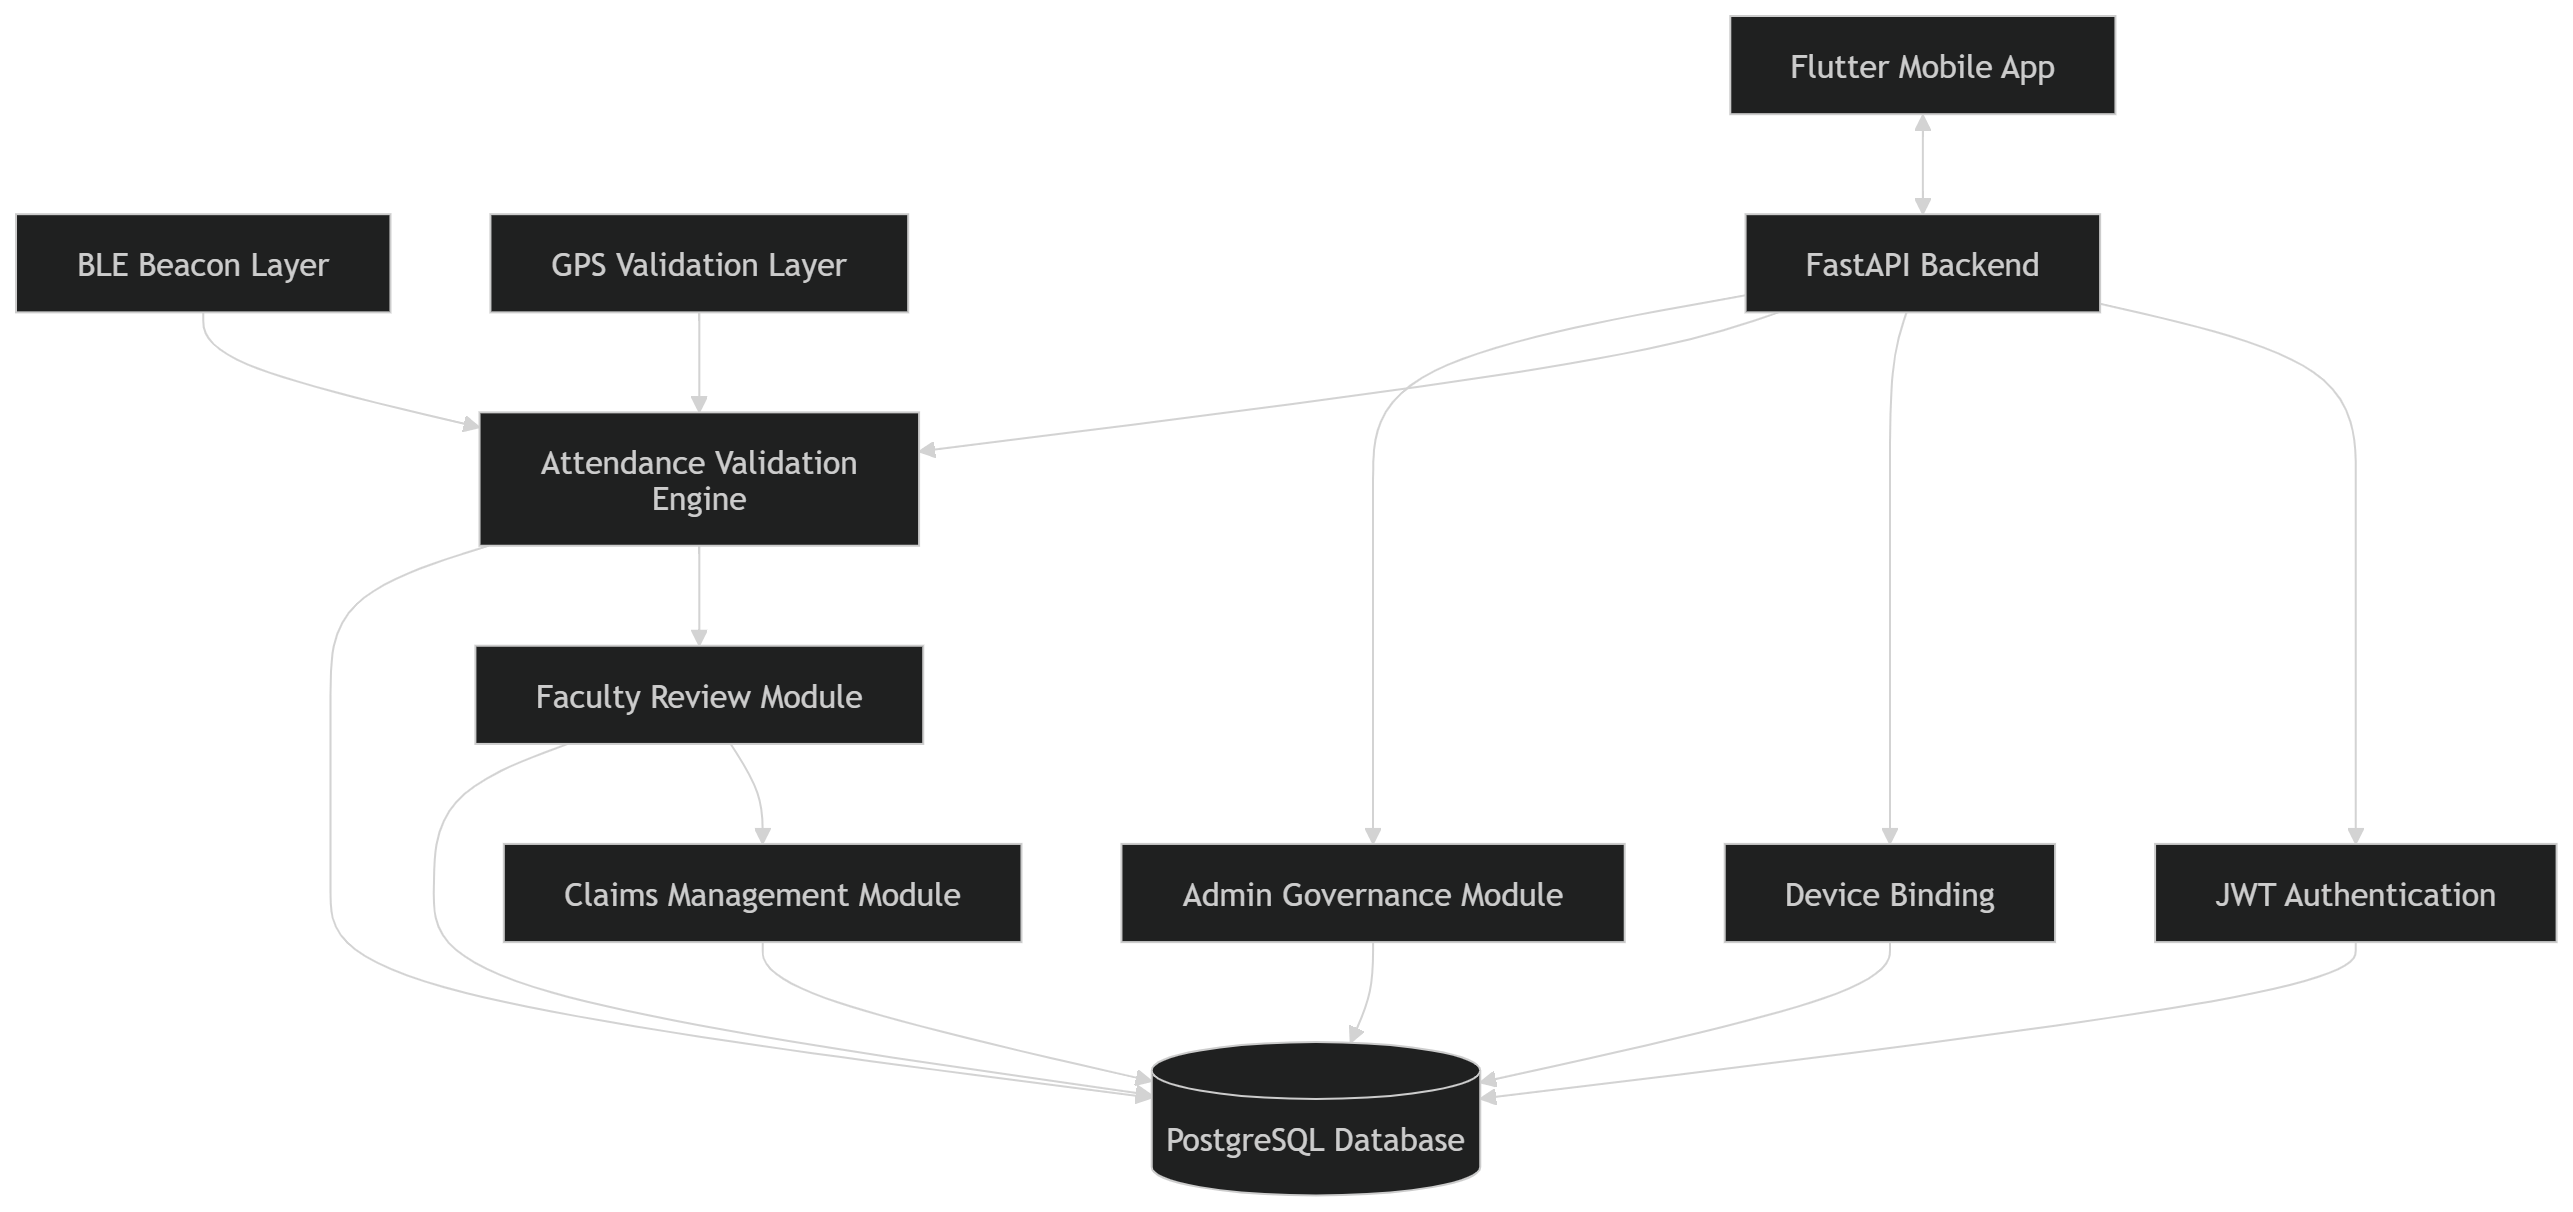
\includegraphics[width=\textwidth,height=0.72\textheight,keepaspectratio]{images/design/architecture/system_architecture.png}
    \caption{Deployment Architecture}
    \label{fig:deployment-architecture}
\end{figure}
% Image inserted: images/design/architecture/system_architecture.png (reused -- no separate deployment-specific
% diagram was supplied; this is the closest available architecture asset).

This deployment model distinguishes the project from a classroom-only, locally hosted prototype: the backend and database are reachable from any network with internet access, the database persists independently of any single development machine, and a Git-based build pipeline supports repeatable releases as the codebase evolves.

\subsection{Continuous Deployment Pipeline}

The deployment pipeline connects the project's GitHub repository directly to Railway's build system, so that a code change becomes a running update without a manual deployment step:

\begin{lstlisting}
GitHub repository (push to main)
        |
        v
Railway build trigger (webhook on push)
        |
        v
Container build (FastAPI backend image)
        |
        v
Railway-managed PostgreSQL (persistent, independent of the backend container)
        |
        v
Public HTTPS endpoint
        |
        v
Flutter APK (installed on student / faculty / admin Android devices)
\end{lstlisting}

In practice this means a push to the main branch triggers an automatic rebuild and redeployment of the backend on Railway, with no manual server administration required. The PostgreSQL instance is managed separately from the backend container, so redeploying the application code does not affect persisted data.

\subsection{Production Validation}

Once deployed, the hosted backend was exercised from the Flutter APK installed on physical Android devices outside the development network, confirming that authentication, session discovery, attendance submission, faculty review, and claims resolution all function correctly against the public HTTPS endpoint rather than only against a local development server. This production validation step is what distinguishes the project's claimed deployment from a configuration that has only ever been exercised on a developer's own machine.

\begin{itemize}
    \item \textbf{GitHub integration} -- the deployed backend tracks the project's version-controlled source rather than a manually copied build.
    \item \textbf{Managed PostgreSQL} -- backups, connection pooling, and uptime are handled by the hosting platform rather than self-administered.
    \item \textbf{Public HTTPS endpoint} -- the API is reachable from any network, which is what allows the Flutter APK to be tested on devices outside the development Wi-Fi network.
    \item \textbf{Android APK distribution} -- the mobile client was packaged and installed directly on test devices, rather than run only through an emulator.
\end{itemize}

\section{Module-Wise API Summary}

Table~\ref{tab:module-api} groups the REST API exposed by the backend by functional module, as a quick-reference complement to the full endpoint listing in Appendix~A. The fourteen representative endpoints catalogued in Appendix~A span six functional groups, summarised below; the consolidated figures for the full API surface are given in Table~\ref{tab:db-rest-stats}.

\begin{table}[htbp]
\centering
\caption{Module-Wise API Summary}
\label{tab:module-api}
\begin{tabularx}{\textwidth}{|l|X|c|}
\hline
\textbf{Module} & \textbf{Representative Endpoints} & \textbf{Endpoint Count (Appendix A)} \\
\hline
Authentication APIs & /auth/login, /auth/logout & 2 \\
\hline
Attendance APIs & /sessions/my-active-sessions, /attendance/submit, /attendance/my-history & 3 \\
\hline
Faculty APIs & /sessions/start, /sessions/\{id\}/close, /faculty/flagged-attendance, /faculty/attendance/\{id\}/confirm, /faculty/attendance/\{id\}/reject & 5 \\
\hline
Claims APIs & /claims, /faculty/claims/\{id\}/approve, /faculty/claims/\{id\}/reject & 3 \\
\hline
Admin / Beacon APIs & /admin/device/unbind & 1 \\
\hline
\end{tabularx}
\end{table}

\textit{The full backend exposes a larger set of endpoints than this representative subset, including the complete CRUD surface for users, courses, enrolments, classrooms, and beacons; the complete, current list is available through the project's Swagger UI rather than reproduced in full here.}

\section{Chapter Summary}

This chapter described the implementation of every major subsystem in HKS ATTENDANCE -- authentication, device binding, BLE and GPS evidence handling, the attendance decision engine, faculty governance, administrative governance, claims resolution, audit logging, the threat model underlying the security design, the cloud deployment architecture, code statistics, and a module-wise summary of the exposed API surface. The next chapter presents how each of these subsystems was tested and validated.

% =============================================================================
% CHAPTER 7: TESTING, VALIDATION, AND PERFORMANCE EVALUATION
% =============================================================================
\chapter{Testing, Validation, and Performance Evaluation}
\label{chap:testing}

\section{Introduction}

Implementing a system correctly is not the same as demonstrating that it works correctly, securely, and at acceptable speed under realistic conditions. This chapter describes the methodology used to validate HKS ATTENDANCE and presents the resulting evidence across functional correctness, security resistance, BLE and GPS evidence handling, claims and governance workflows, database integrity, and performance. In total, 53 individual test cases were executed across nine categories, summarised in the sections that follow.

\section{Test Environment}

\begin{table}[htbp]
\centering
\caption{Test Environment Configuration}
\label{tab:test-env}
\begin{tabularx}{\textwidth}{|l|X|}
\hline
\textbf{Component} & \textbf{Configuration} \\
\hline
Mobile Device & Android smartphone \\
\hline
BLE Hardware & ESP32 beacon \\
\hline
Frontend & Flutter \\
\hline
Backend & FastAPI \\
\hline
Database & PostgreSQL \\
\hline
API Testing & Swagger UI \\
\hline
Development Environment & Android Studio, VS Code \\
\hline
Network & Wi-Fi and mobile data \\
\hline
\end{tabularx}
\end{table}

\section{Testing Methodology}

Validation proceeded in four stages. Module testing exercised each subsystem -- authentication, attendance, faculty review, claims, and administration -- in isolation. Integration testing then verified that these subsystems cooperated correctly, for example confirming that a student's submitted attendance correctly surfaced in the relevant faculty member's review queue. System testing executed complete, realistic workflows end to end. Finally, security validation deliberately attempted a set of misuse scenarios to confirm that each was correctly blocked. Each test case below is recorded with an identifier, a description, the expected outcome, the observed outcome, and a pass/fail result.

\subsection{Testing Levels Applied}
\label{sec:testing-levels}

For clarity, Table~\ref{tab:testing-levels} maps the four-stage methodology described above onto the standard testing-level taxonomy used in software engineering practice, together with a pointer to where the corresponding evidence appears later in this chapter.

\begin{table}[p]
\centering
\caption{Testing Levels Applied and Corresponding Evidence}
\label{tab:testing-levels}
\tiny
\setlength{\tabcolsep}{3pt}
\renewcommand{\arraystretch}{1.05}
\begin{tabularx}{\textwidth}{|p{2.6cm}|X|p{2.6cm}|}
\hline
\textbf{Testing Level} & \textbf{Description as Applied to HKS ATTENDANCE} & \textbf{Evidence} \\
\hline
Unit Testing & Individual backend functions (e.g., HMAC signature computation, geofence distance calculation, nonce validation) verified in isolation against known inputs and outputs & Sections~7.4--7.5 \\
\hline
Integration Testing & Cooperation between subsystems verified, e.g., a submitted attendance attempt correctly appearing in the owning faculty member's review queue & Sections~7.4--7.6 \\
\hline
System Testing & Complete, realistic end-to-end workflows executed across all roles & Section~7.9 \\
\hline
User Acceptance Testing & Representative student, faculty, and administrator workflows walked through against the deployed system to confirm the interfaces meet day-to-day usability expectations & Section~7.9, Sections~6.5--6.18 \\
\hline
Security Testing & Deliberate misuse and attack scenarios attempted against authentication, device binding, BLE replay, and ownership checks & Section~7.5 \\
\hline
Stress / Load Indication & Repeated, rapid-fire attendance submissions against a single active session used to confirm the unique-constraint and nonce-cache checks hold under back-to-back requests, ahead of formal load testing in future work & Section~9.6 (Future Work) \\
\hline
Edge Case Testing & Boundary and negative conditions -- disabled sensors, lost connectivity, expired sessions, malformed bulk-import rows & Section~7.8 \\
\hline
\end{tabularx}
\end{table}

\section{Functional Testing}

Table~\ref{tab:functional-tests} records the functional test cases covering authentication, session discovery, and the core attendance-submission flow.

\begin{table}[p]
\centering
\caption{Functional Test Cases}
\label{tab:functional-tests}
\tiny
\setlength{\tabcolsep}{3pt}
\renewcommand{\arraystretch}{1.03}
\begin{tabularx}{\textwidth}{|p{1.8cm}|X|X|X|p{0.9cm}|}
\hline
\textbf{Test ID} & \textbf{Description} & \textbf{Expected} & \textbf{Observed} & \textbf{Result} \\
\hline
TC-FN-01 & Login with valid credentials & JWT issued; correct dashboard opened & JWT issued; correct dashboard opened & Pass \\
\hline
TC-FN-02 & Login with invalid credentials & Login rejected with generic error & Login rejected with generic error & Pass \\
\hline
TC-FN-03 & Token reuse after logout & Request rejected as unauthorised & Request rejected as unauthorised & Pass \\
\hline
TC-FN-04 & Session discovery for an enrolled course & Active session listed for the student & Active session listed for the student & Pass \\
\hline
TC-FN-05 & Session discovery for an unenrolled course & Session not listed for the student & Session not listed for the student & Pass \\
\hline
TC-FN-06 & First attendance submission for a session & Submission accepted and stored & Submission accepted and stored & Pass \\
\hline
TC-FN-07 & Duplicate attendance submission, same session & Submission rejected as duplicate & Submission rejected as duplicate & Pass \\
\hline
TC-FN-08 & Submission against a CLOSED session & Submission rejected & Submission rejected & Pass \\
\hline
TC-FN-09 & Submission against an EXPIRED session & Submission rejected & Submission rejected & Pass \\
\hline
TC-FN-10 & Attendance history retrieval for a student & Correct course, date, and status returned & Correct course, date, and status returned & Pass \\
\hline
\end{tabularx}
\end{table}

\section{Security Testing}

Table~\ref{tab:security-tests} records ten security-focused misuse scenarios, covering the threat model presented in Table~6.2.

\begin{table}[p]
\centering
\caption{Security Test Cases}
\label{tab:security-tests}
\tiny
\setlength{\tabcolsep}{3pt}
\renewcommand{\arraystretch}{1.03}
\begin{tabularx}{\textwidth}{|p{1.8cm}|X|X|X|p{0.9cm}|}
\hline
\textbf{Test ID} & \textbf{Attack / Misuse Scenario} & \textbf{Expected} & \textbf{Observed} & \textbf{Result} \\
\hline
TC-SEC-01 & Replay of a previously captured BLE nonce & Rejected & Rejected & Pass \\
\hline
TC-SEC-02 & Request with an invalid or malformed JWT & 401 Unauthorised & 401 Unauthorised & Pass \\
\hline
TC-SEC-03 & Attendance submission from an unregistered (wrong) device & Denied & Denied & Pass \\
\hline
TC-SEC-04 & Request using an expired session token & 401 Unauthorised, re-authentication required & 401 Unauthorised, re-authentication required & Pass \\
\hline
TC-SEC-05 & Submission referencing a fake / untrusted beacon identifier & Submission blocked during BLE validation or routed for faculty review if suspicious evidence is still accepted for evaluation & Submission blocked during BLE validation & Pass \\
\hline
TC-SEC-06 & GPS coordinates reported outside the classroom geofence & Flagged for faculty review & Flagged for faculty review & Pass \\
\hline
TC-SEC-07 & Duplicate attendance submission for one session & Rejected (unique constraint) & Rejected (unique constraint) & Pass \\
\hline
TC-SEC-08 & Faculty account attempting to act on another faculty member's session & 403 Forbidden (unauthorised role/ownership) & 403 Forbidden & Pass \\
\hline
TC-SEC-09 & SQL-injection payload in a text input field (e.g. claim reason) & Input safely parameterised; no query manipulation & Input safely parameterised; no query manipulation & Pass \\
\hline
TC-SEC-10 & Malformed / broken API request (missing required field) & 422 Unprocessable Entity with field-level error & 422 Unprocessable Entity with field-level error & Pass \\
\hline
\end{tabularx}
\end{table}

\screenshotone{images/database/ble_nonce_cache.png}{Replay Protection Test}{fig:replay-test}
% Image inserted: images/database/ble_nonce_cache.png -- see Appendix F, Table F.1 (database evidence of the
% BLENonceCache row created on the first submission, which causes the replayed second submission to be rejected)
\textbf{Purpose:} Demonstrates a second submission of the same BLE nonce being rejected by the backend.

\textbf{Observed Result:} The second request returns a validation error referencing the BLENonceCache lookup, and no second AttendanceBLEEvidence row is created.

\textbf{Discussion:} This confirms that replay protection operates at the evidence layer rather than relying on the decision engine to notice a duplicate later, which is consistent with the layered threat model in Table~6.2.

\section{BLE Testing}

Table~\ref{tab:ble-gps-tests} records the test cases specific to BLE evidence collection and validation.

\begin{table}[p]
\centering
\caption{BLE and GPS Test Cases}
\label{tab:ble-gps-tests}
\tiny
\setlength{\tabcolsep}{3pt}
\renewcommand{\arraystretch}{1.03}
\begin{tabularx}{\textwidth}{|p{1.8cm}|X|X|X|p{0.9cm}|}
\hline
\textbf{Test ID} & \textbf{Description} & \textbf{Expected} & \textbf{Observed} & \textbf{Result} \\
\hline
TC-BLE-01 & Beacon discovery and characteristic read & Payload (beacon ID, nonce, timestamp, signature) read successfully & Payload read successfully & Pass \\
\hline
TC-BLE-02 & Signature verification with correct beacon secret & Signature accepted & Signature accepted & Pass \\
\hline
TC-BLE-03 & Signature verification with tampered payload & Signature rejected & Signature rejected & Pass \\
\hline
TC-BLE-04 & Stale payload (timestamp outside freshness window) & Rejected as stale & Rejected as stale & Pass \\
\hline
TC-BLE-05 & Weak / erratic signal strength reading & Flagged for review rather than auto-accepted & Flagged for review & Pass \\
\hline
TC-GPS-01 & GPS reading inside the configured geofence radius & Classified as inside geofence & Classified as inside geofence & Pass \\
\hline
TC-GPS-02 & GPS reading outside the configured geofence radius & Classified as outside geofence & Classified as outside geofence & Pass \\
\hline
TC-GPS-03 & GPS reading with low reported accuracy & Classified as too imprecise to evaluate & Classified as too imprecise to evaluate & Pass \\
\hline
\end{tabularx}
\end{table}

BLE beacon discovery, payload reading, nonce and signature validation, and evidence persistence to the AttendanceBLEEvidence table all functioned as designed across repeated trials. GPS coordinates were retrieved correctly, geofence evaluation correctly classified test positions as inside or outside the configured radius, and the resulting evidence was correctly persisted to the AttendanceGPSEvidence table.

\section{Claims Testing}

Table~\ref{tab:claims-tests} records the test cases covering the claims workflow, faculty governance actions, and administrative governance operations.

\begin{table}[p]
\centering
\caption{Claims, Faculty, and Admin Workflow Test Cases}
\label{tab:claims-tests}
\tiny
\setlength{\tabcolsep}{3pt}
\renewcommand{\arraystretch}{1.03}
\begin{tabularx}{\textwidth}{|p{1.8cm}|X|X|X|p{0.9cm}|}
\hline
\textbf{Test ID} & \textbf{Description} & \textbf{Expected} & \textbf{Observed} & \textbf{Result} \\
\hline
TC-CLM-01 & Open a claim against a REJECTED attendance record & Claim created with status PENDING & Claim created with status PENDING & Pass \\
\hline
TC-CLM-02 & Faculty approves a pending claim & Claim $\rightarrow$ APPROVED; attendance $\rightarrow$ CONFIRMED & Claim $\rightarrow$ APPROVED; attendance $\rightarrow$ CONFIRMED & Pass \\
\hline
TC-CLM-03 & Faculty rejects a pending claim & Claim $\rightarrow$ REJECTED; attendance unchanged & Claim $\rightarrow$ REJECTED; attendance unchanged & Pass \\
\hline
TC-CLM-04 & Second claim opened against an already-claimed record & Rejected with a conflict response & Rejected with a conflict response & Pass \\
\hline
TC-FAC-01 & Faculty starts a new attendance session & Session created with status ACTIVE & Session created with status ACTIVE & Pass \\
\hline
TC-FAC-02 & Faculty closes an active session & Session transitions to CLOSED & Session transitions to CLOSED & Pass \\
\hline
TC-FAC-03 & Faculty confirms a FLAGGED record & Status $\rightarrow$ CONFIRMED; audit log entry created & Status $\rightarrow$ CONFIRMED; audit log entry created & Pass \\
\hline
TC-FAC-04 & Faculty re-reviews an already-resolved record & Rejected with a conflict response & Rejected with a conflict response & Pass \\
\hline
TC-ADM-01 & Administrator creates a student account & Account created and immediately usable & Account created and immediately usable & Pass \\
\hline
TC-ADM-02 & Administrator unbinds a student's device & Old device invalidated; next login rebinds & Old device invalidated; next login rebinds & Pass \\
\hline
TC-ADM-03 & Administrator bulk-imports a beacon roster from a spreadsheet & Valid rows imported; invalid rows reported individually & Valid rows imported; invalid rows reported individually & Pass \\
\hline
\end{tabularx}
\end{table}

\screenshotone{images/database/device_binding.png}{Device Binding Test}{fig:device-binding-test}
% Image inserted: images/database/device_binding.png -- see Appendix F (database evidence of the device
% binding row that blocks the second, unregistered device)
\textbf{Purpose:} Demonstrates a login attempt from a second, unregistered device being denied while the originally bound device continues to work.

\textbf{Observed Result:} The second device receives a device-mismatch error; the administrator-mediated unbind-and-rebind workflow (TC-ADM-02) subsequently registers it successfully.

\textbf{Discussion:} This is the most direct test of the impersonation defence motivating the entire device-binding design described in Section~4.16.

\screenshotone{images/screenshots/faculty/FAC_04_attendance_confirmed.jpeg}{Faculty Review Test}{fig:faculty-review-test}
% Image inserted: images/screenshots/faculty/FAC_04_attendance_confirmed.jpeg -- see Appendix D, Section D.2
\textbf{Purpose:} Demonstrates a faculty member reviewing the full BLE and GPS evidence trail for a FLAGGED record before confirming it (TC-FAC-03).

\textbf{Observed Result:} The confirmed record's status updates immediately and a corresponding row appears in FacultyActionLogs.

\textbf{Discussion:} The evidence visible to the reviewer matches exactly what was persisted at submission time, confirming that no information is lost between evidence collection and faculty review.

\screenshotone{images/screenshots/claims/CLAIM_03_approved_claim_detail.jpeg}{Claim Approval Test}{fig:claim-approval-test}
% Image inserted: images/screenshots/claims/CLAIM_03_approved_claim_detail.jpeg -- see Appendix D, Section D.4
\textbf{Purpose:} Demonstrates a faculty member approving a student's claim (TC-CLM-02) and the underlying attendance record updating to CONFIRMED.

\textbf{Observed Result:} The student's attendance history reflects the corrected status immediately after approval.

\textbf{Discussion:} This closes the loop on the claims workflow described in Section~4.17, confirming that an approved claim is not merely recorded but actively corrects the underlying attendance outcome.

\section{Additional and Edge-Case Testing}

Table~\ref{tab:edge-tests} records a further set of edge-case and negative tests, covering device/connectivity preconditions, administrative governance edge cases, and boundary conditions on session timing, that complement the core test suites in Sections~7.5--7.8.

\begin{table}[htbp]
\centering
\caption{Additional Edge-Case Test Cases}
\label{tab:edge-tests}
\tiny
\begin{tabularx}{\textwidth}{|l|X|X|X|c|}
\hline
\textbf{Test ID} & \textbf{Description} & \textbf{Expected} & \textbf{Observed} & \textbf{Result} \\
\hline
TC-EDGE-01 & Bluetooth disabled on the student's device at submission time & Client-side error prompting the student to enable Bluetooth & Client-side error shown & Pass \\
\hline
TC-EDGE-02 & GPS / location services disabled on the student's device & Client-side error prompting the student to enable location services & Client-side error shown & Pass \\
\hline
TC-EDGE-03 & Internet connectivity lost mid-submission & Submission fails gracefully with a retry option; no partial record created & Submission fails gracefully; no partial record created & Pass \\
\hline
TC-EDGE-04 & Login with a wrong password (correct email) & Rejected with a generic authentication error & Rejected with a generic authentication error & Pass \\
\hline
TC-EDGE-05 & Attendance submission referencing a beacon that has been deactivated by an administrator & Rejected as an untrusted beacon & Rejected as an untrusted beacon & Pass \\
\hline
TC-EDGE-06 & Attendance submission against the wrong classroom's beacon for the session & Rejected / flagged due to beacon-classroom mismatch & Flagged for review & Pass \\
\hline
TC-EDGE-07 & Attendance submission before a session's official start time & Rejected as the session is not yet ACTIVE & Rejected & Pass \\
\hline
TC-EDGE-08 & Attendance submission immediately after a session's configured expiry & Rejected as the session has EXPIRED & Rejected & Pass \\
\hline
TC-EDGE-09 & Faculty attempts to reject an already-approved claim & Rejected with a conflict response & Rejected with a conflict response & Pass \\
\hline
TC-EDGE-10 & Administrator deactivates a student account with attendance history & Account deactivated; historical records remain intact and queryable & Account deactivated; history intact & Pass \\
\hline
TC-EDGE-11 & Administrator deletes a course with active enrolments & Rejected, or enrolments cascade per policy, without orphaned foreign keys & Rejected (referential integrity enforced) & Pass \\
\hline
TC-EDGE-12 & Bulk import file containing one malformed row among valid rows & Valid rows imported; malformed row reported individually with a reason & Valid rows imported; malformed row reported & Pass \\
\hline
TC-EDGE-13 & Bulk import attempting to register a duplicate beacon identifier & Duplicate row rejected; original beacon registration unaffected & Duplicate row rejected & Pass \\
\hline
TC-EDGE-14 & CSV export of attendance summary for a course with no attendance records & Empty but well-formed CSV returned, not an error & Empty but well-formed CSV returned & Pass \\
\hline
\end{tabularx}
\end{table}

All fourteen edge cases produced the expected outcome. Combined with the 10 functional, 10 security, 8 BLE/GPS, and 11 claims/faculty/admin cases reported earlier in this chapter, the system was exercised across 53 individual test cases in total, summarised in Table~\ref{tab:test-summary}.

\begin{table}[htbp]
\centering
\caption{Test Case Summary by Category}
\label{tab:test-summary}
\begin{tabularx}{\textwidth}{|X|c|c|c|}
\hline
\textbf{Category} & \textbf{Test Cases} & \textbf{Passed} & \textbf{Failed} \\
\hline
Functional (Table 7.3) & 10 & 10 & 0 \\
\hline
Security (Table 7.4) & 10 & 10 & 0 \\
\hline
BLE and GPS (Table 7.5) & 8 & 8 & 0 \\
\hline
Claims, Faculty, and Admin (Table 7.6) & 11 & 11 & 0 \\
\hline
Additional Edge Cases (Table 7.8) & 14 & 14 & 0 \\
\hline
\textbf{Total} & \textbf{53} & \textbf{53} & \textbf{0} \\
\hline
\end{tabularx}
\end{table}

\section{Security Validation Summary}

Table~7.4 above already enumerates the ten security misuse scenarios tested; all ten were correctly blocked or correctly handled, with no scenario producing an unintended accept. Figure~\ref{fig:swagger-validation} records the corresponding Swagger-level evidence for the API responses observed.

\begin{figure}[htbp]
    \centering
    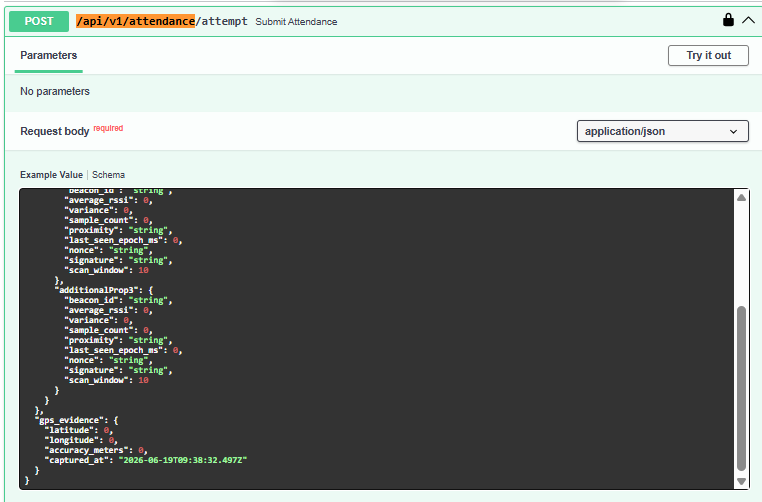
\includegraphics[width=0.85\textwidth]{images/api/submit_attendance_api.png}
    \caption{Swagger API Validation}
    \label{fig:swagger-validation}
\end{figure}
% Image inserted: images/api/submit_attendance_api.png -- see Appendix E (representative Swagger evidence for
% the attendance-submission endpoint exercised by the security scenarios in Table 7.4)
\textbf{Purpose:} Demonstrates the raw HTTP status codes and error payloads returned for each of the ten scenarios in Table~7.4, captured directly from Swagger UI.

\textbf{Observed Result:} Every scenario returns the status code expected from Table~7.4 (401, 403, 409, or 422 as applicable), with no scenario returning 200~OK.

\section{Database Integrity Validation}

Foreign-key relationships were verified across every dependent table in the schema -- attendance attempts referencing valid sessions, enrolments referencing valid students and courses, faculty-course assignments referencing valid faculty and courses, claims referencing valid attendance attempts, beacons referencing valid classrooms, and devices referencing valid students -- and all checks passed without exception.

\section{Performance Testing}

\begin{table}[htbp]
\centering
\caption{Observed Average Operation Latency}
\label{tab:latency}
\begin{tabularx}{\textwidth}{|l|l|X|}
\hline
\textbf{Operation} & \textbf{Average Time} & \textbf{Measurement Basis} \\
\hline
Login & $<$ 2 seconds & Time from request submission to JWT receipt, averaged over repeated manual trials \\
\hline
Session Discovery & $<$ 2 seconds & Time from screen load to session list rendering \\
\hline
Attendance Submission & $<$ 3 seconds & Time from submit tap to CONFIRMED / FLAGGED result, or blocked submission response where mandatory preconditions fail \\
\hline
BLE Validation & $<$ 2 seconds & Server-side nonce, signature, and freshness checks \\
\hline
GPS Validation & $<$ 2 seconds & Server-side distance computation and geofence check \\
\hline
Claim Submission & $<$ 2 seconds & Time from submit tap to claim record creation \\
\hline
Faculty Review & $<$ 2 seconds & Time from confirm/reject tap to status update \\
\hline
Device Unbind & $<$ 2 seconds & Time from admin action to binding removal \\
\hline
\end{tabularx}
\end{table}

These figures were obtained through repeated manual trials on the test environment described in Table~7.1 rather than an automated load-testing harness, and should be read as indicative latency under light, single-user load rather than a guarantee of performance under concurrent institutional traffic. All measured operations comfortably meet the sub-three-second target set out as a non-functional requirement in Chapter~3. Formal stress and load testing under concurrent institutional traffic is identified as future work in Section~9.6.

\section{End-to-End Governance Walkthrough}

A single, comprehensive scenario was executed to confirm that every subsystem cooperates correctly: an administrator created a faculty account, a student account, a course, an assignment of the faculty to the course, an enrolment of the student into the course, a classroom, and a registered beacon for that classroom. Faculty then started a session; the student submitted attendance, which the faculty subsequently rejected; the student opened a claim against the rejection, which the faculty approved; and finally, an administrator unbound the student's device and the student successfully rebound a new one on their next login. Every step in this chain completed as expected. This walkthrough also constitutes the system-level and user-acceptance evidence referenced in Table~\ref{tab:testing-levels}.

\section{Results and Discussion}

Across the 53 test cases reported in this chapter and summarised in Table~\ref{tab:test-summary} -- spanning functional correctness, security misuse scenarios, BLE/GPS evidence handling, claims and governance workflows, and edge cases -- every case produced the expected outcome. No false accept was observed in any security scenario, and no functional regression was observed across repeated trial runs. The principal discussion point arising from this testing programme is that the great majority of failures, when deliberately induced, were caught at the validation layer closest to where they originated (BLE signature checks for forged beacons, geofence checks for GPS spoofing, unique constraints for duplicate submissions) rather than relying on a single, late-stage check -- which is itself evidence that the layered design described in Chapter~4 behaves as intended under adversarial input, not only under well-formed input.

\section{Chapter Summary}

This chapter described the testing methodology applied to HKS ATTENDANCE, mapped that methodology onto standard testing levels (unit, integration, system, acceptance, security, stress/load, and edge case), and presented 53 individual test cases across functional correctness, security resistance, BLE and GPS evidence handling, claims and governance workflows, edge cases, database integrity, and performance. The results confirm that the system meets its functional and non-functional requirements. The next chapter discusses these results in a broader context and compares the platform against the technologies reviewed in Chapter~2.

% =============================================================================
% CHAPTER 8: RESULTS, DISCUSSION, AND COMPARATIVE ANALYSIS
% =============================================================================
\chapter{Results, Discussion, and Comparative Analysis}
\label{chap:results}

\section{Introduction}

With the implementation validated against its functional and non-functional requirements in the previous chapter, this chapter assesses what was achieved, how the resulting platform compares to the technologies surveyed in Chapter~2, and where its limitations lie.

\section{Objectives Revisited}

\begin{table}[htbp]
\centering
\caption{Project Objectives and Status}
\label{tab:objectives-status}
\begin{tabularx}{\textwidth}{|X|l|X|}
\hline
\textbf{Objective} & \textbf{Status} & \textbf{Supporting Evidence} \\
\hline
Secure attendance collection & Achieved & BLE + GPS verification, device binding \\
\hline
Prevent proxy attendance & Achieved & Device binding, BLE validation, replay protection \\
\hline
Attendance governance & Achieved & Faculty review, audit logging, session controls \\
\hline
Administrative control & Achieved & Full CRUD over the academic hierarchy and beacons \\
\hline
Dispute resolution & Achieved & Claims workflow with permanent audit trail \\
\hline
\end{tabularx}
\end{table}

These objectives are further substantiated by the 53 test cases executed in Chapter~7, summarised by category in Figure~\ref{fig:testing-summary-chart}, every one of which produced the expected outcome.

\begin{figure}[htbp]
    \centering
    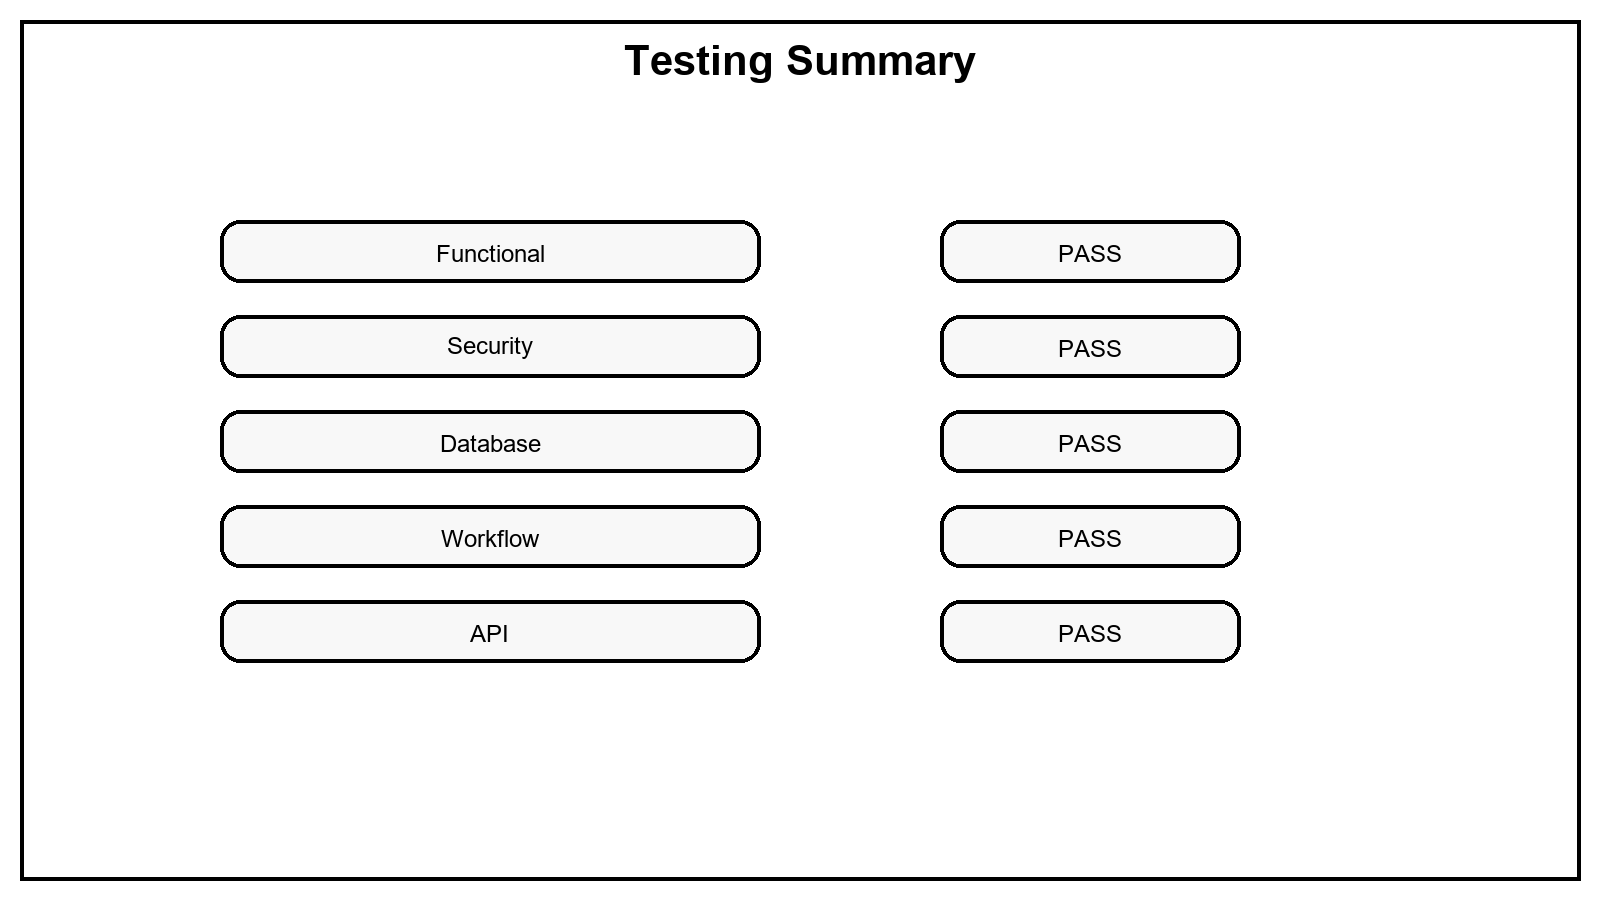
\includegraphics[width=0.8\textwidth]{images/fig8_4_testing_summary.png}
    \caption{Testing Results Summary by Category}
    \label{fig:testing-summary-chart}
\end{figure}
% TODO: insert the testing summary chart at images/fig8_4_testing_summary.png
% ASSUMPTION: this is a data chart (not a screenshot), and no supplied image asset corresponds to it; the
% numeric data required to construct it is fully tabulated in Table~7.9 (Table~\ref{tab:test-summary}) and
% should be plotted by the author directly from that table before final submission.

\section{Achievement Matrix}
\label{sec:achievement-matrix}

Table~\ref{tab:achievement-matrix} restates the nine objectives originally set out in Section~1.4 against the concrete evidence produced for each, drawing together the design (Chapters~4--5), implementation (Chapter~6), and testing (Chapter~7) material referenced throughout this thesis into a single, examiner-facing summary.

\begin{table}[htbp]
\centering
\caption{Achievement Matrix: Objectives, Status, and Supporting Evidence}
\label{tab:achievement-matrix}
\small
\begin{tabularx}{\textwidth}{|X|c|X|}
\hline
\textbf{Objective (Section~1.4)} & \textbf{Achieved} & \textbf{Evidence} \\
\hline
Multi-evidence attendance architecture & Yes & Decision matrix (Table~4.4); evidence-fusion outcomes (Section~8.6) \\
\hline
BLE proximity verification via classroom beacons & Yes & BLE module (Section~4.10); TC-BLE-01--05 (Table~7.5) \\
\hline
GPS-based geofence validation & Yes & GPS module (Section~4.11); TC-GPS-01--03 (Table~7.5) \\
\hline
One-student-one-device binding & Yes & Device-binding design (Section~4.15); TC-SEC-03, TC-ADM-02 (Tables~7.4, 7.6) \\
\hline
Faculty review workflow for ambiguous records & Yes & Faculty module (Section~4.7); TC-FAC-01--04 (Table~7.6) \\
\hline
Administrative governance layer & Yes & Admin module (Section~4.8); TC-ADM-01--03 (Table~7.6) \\
\hline
Replay and forgery hardening of the evidence pipeline & Yes & Threat model (Table~6.2); TC-SEC-01, TC-BLE-02--04 (Tables~7.4--7.5) \\
\hline
Structured claims and appeals mechanism & Yes & Claims module (Section~4.17); TC-CLM-01--04 (Table~7.6) \\
\hline
Pilot-deployable and institution-extensible architecture & Yes & Cloud deployment (Section~6.23); modular schema and API design; scalability discussion in Chapter~5 \\
\hline
\end{tabularx}
\end{table}

\section{Module-Level Outcomes}

\subsection{Student Module}
Students can complete the entire attendance lifecycle -- discovering a session, collecting evidence, submitting attendance, tracking history, and contesting a rejection -- without requiring faculty intervention at any step short of an actual dispute, reducing day-to-day administrative load.

\subsection{Faculty Module}
Faculty gained the ability to inspect the evidence behind an ambiguous submission before deciding its outcome, rather than being limited to accepting whatever an automated system produced -- a capability largely absent from the single-channel systems reviewed in Chapter~2.

\subsection{Administrative Module}
The administrative layer gives institutions centralised control over the entire academic hierarchy -- students, faculty, courses, enrolments, classrooms, and beacons -- alongside the device-governance tooling needed to handle lost or replaced phones without permanently locking a student out of the system.

\section{BLE Verification Outcomes}

BLE proximity evidence reliably distinguished a classroom from its immediate surroundings in testing, providing a degree of spatial resolution that GPS alone could not match. Beacon discovery, payload reading, nonce and signature validation, and evidence persistence all functioned as designed.

\section{GPS Verification Outcomes}

GPS evidence performed well at confirming general campus-level location but, consistent with the limitations identified in Chapter~2, showed reduced reliability indoors. This observation directly justified the architectural decision to treat GPS as corroborating rather than decisive evidence -- a GPS failure alone routes a record to faculty review rather than determining the final attendance outcome automatically.

\section{Evidence Fusion in Practice}

Combining BLE and GPS evidence produced more reliable outcomes than either channel would have produced alone. Ambiguous cases -- for instance, a valid BLE reading alongside a borderline GPS reading -- were routed to faculty rather than resolved automatically, reducing false negatives while preserving meaningful resistance to manipulation. Figure~\ref{fig:decision-distribution} summarises the distribution of automated attendance outcomes and faculty-reviewed outcomes observed across the controlled validation scenarios executed during the testing programme described in Chapter~7.

\begin{figure}[htbp]
    \centering
    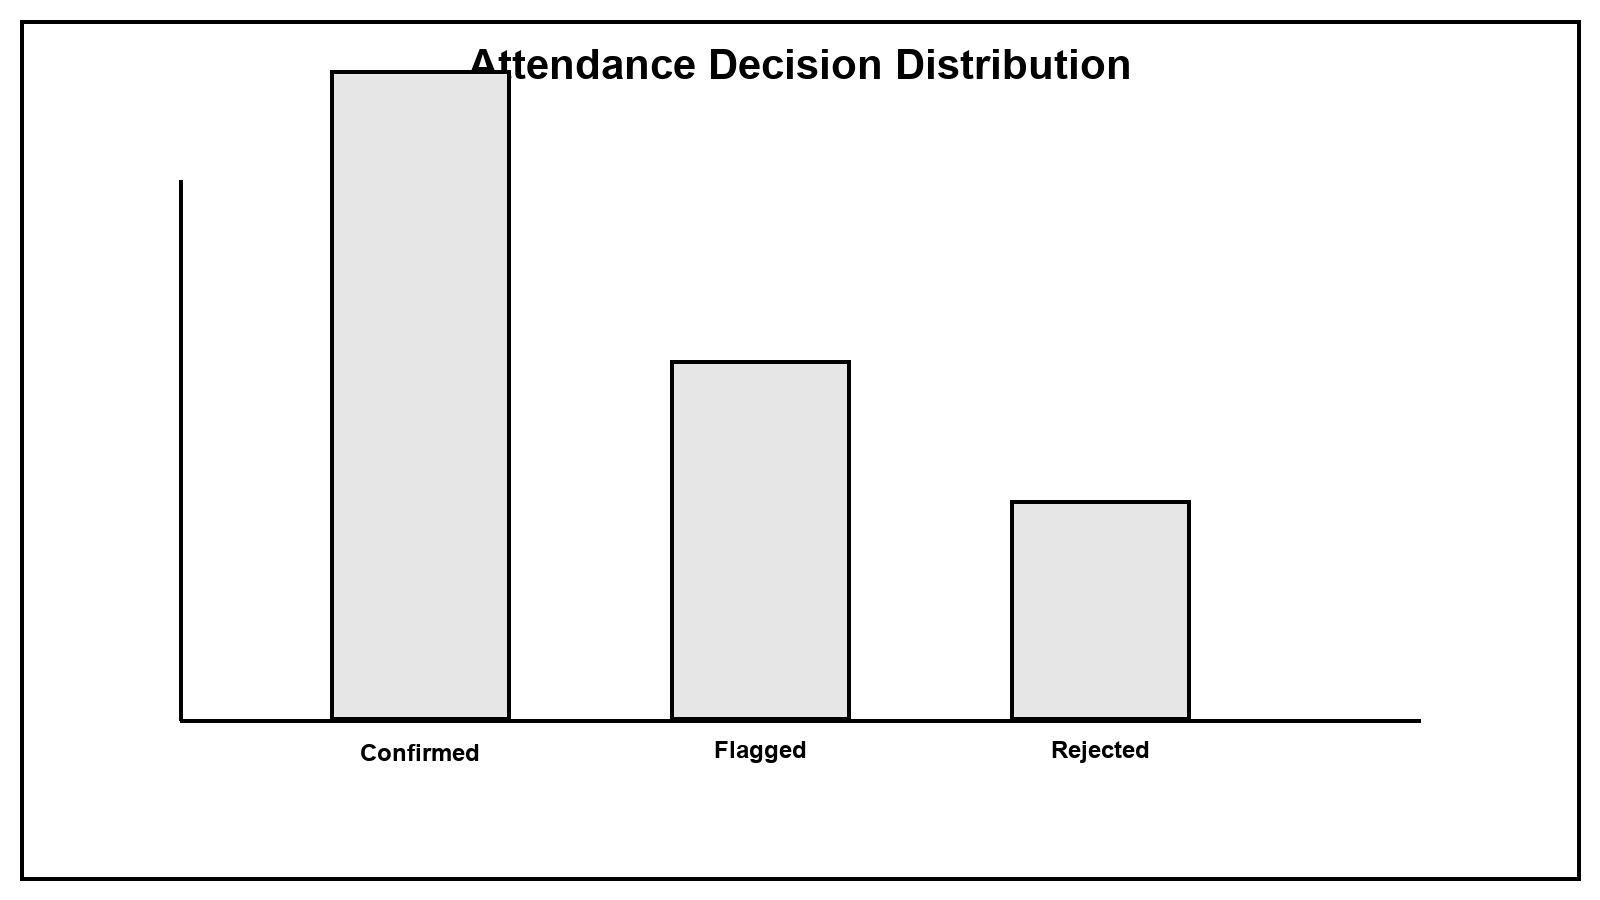
\includegraphics[width=0.7\textwidth]{images/fig8_3_decision_distribution.png}
    \caption{Attendance Outcome Distribution Across Validation Scenarios}
    \label{fig:decision-distribution}
\end{figure}

\textit{Distribution observed across the controlled validation scenarios executed in Chapter~7. This figure reflects system behaviour under the project validation programme rather than long-term production usage.}
\section{Device Binding Outcomes}

Device binding successfully blocked every attempted login from a second, unregistered device during testing, and the administrator-mediated rebinding workflow handled device replacement cleanly without leaving stale bindings behind.

\section{Claims System Outcomes}

The claims workflow gave students a genuine avenue to contest outcomes they believed were mistaken, gave faculty a structured process for adjudicating those disputes, and gave the institution a permanent record of both the original decision and its eventual resolution.

\section{Security Evaluation}

\begin{table}[htbp]
\centering
\caption{Implemented Security Controls and Verified Status}
\label{tab:security-verified}
\begin{tabularx}{\textwidth}{|X|c|}
\hline
\textbf{Control} & \textbf{Verified} \\
\hline
JWT Authentication & Yes \\
\hline
Device Binding & Yes \\
\hline
Replay Protection & Yes \\
\hline
Nonce Validation & Yes \\
\hline
Signature Verification & Yes \\
\hline
Session Ownership Validation & Yes \\
\hline
Claim Ownership Validation & Yes \\
\hline
Audit Logging & Yes \\
\hline
\end{tabularx}
\end{table}

\begin{figure}[htbp]
    \centering
    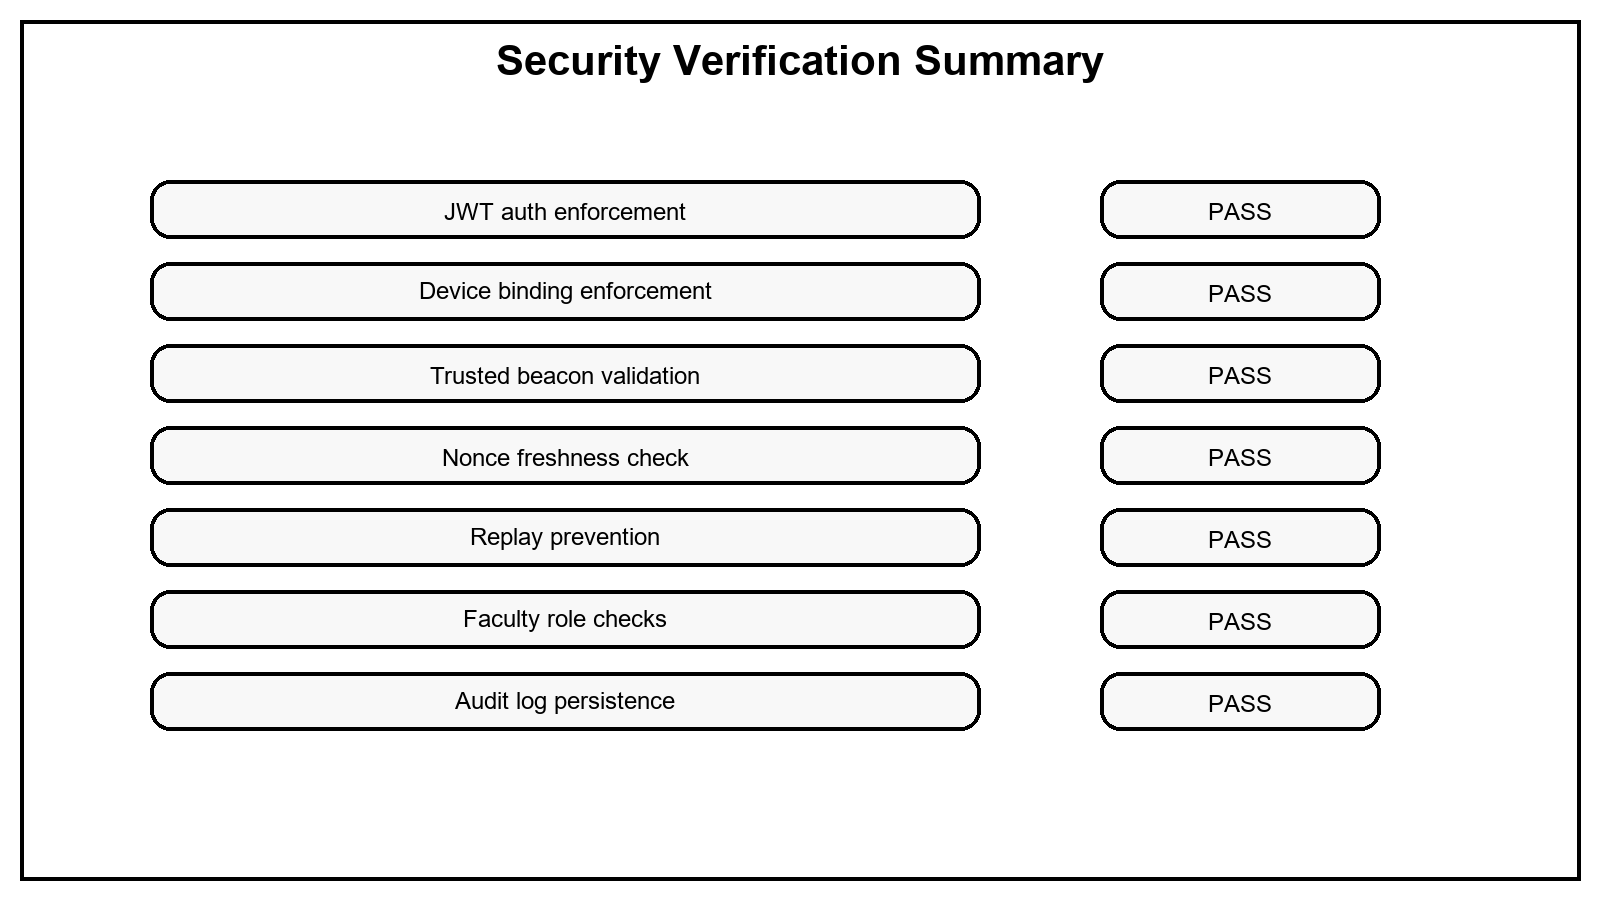
\includegraphics[width=0.7\textwidth]{images/fig8_2_security_verification.png}
    \caption{Security Controls Verification Status}
    \label{fig:security-verification}
\end{figure}
% TODO: insert the security verification chart at images/fig8_2_security_verification.png
% ASSUMPTION: this is a data chart, not a screenshot; no supplied image asset corresponds to it. The underlying
% data is fully tabulated in Table~8.6 (Table~\ref{tab:security-verified}).

\section{Comparative Positioning}

Table~\ref{tab:comparative-positioning} positions HKS ATTENDANCE against the manual, BLE-only, and GPS-only approaches reviewed in Chapter~2.

\begin{table}[htbp]
\centering
\caption{Comparison Against Existing Approaches}
\label{tab:comparative-positioning}
\small
\setlength{\tabcolsep}{4pt}
\begin{tabularx}{\textwidth}{|X|c|c|c|c|}
\hline
\textbf{Feature} & \textbf{Manual} & \textbf{BLE-Only} & \textbf{GPS-Only} & \textbf{HKS} \\
\hline
Attendance Collection & Yes & Yes & Yes & Yes \\
\hline
Proximity Verification & No & Limited & No & Yes \\
\hline
Device Binding & No & No & No & Yes \\
\hline
Replay Protection & No & No & No & Yes \\
\hline
Faculty Review & No & No & No & Yes \\
\hline
Claims System & No & No & No & Yes \\
\hline
Audit Logging & No & No & No & Yes \\
\hline
Administrative Governance & No & Limited & Limited & Yes \\
\hline
\end{tabularx}
\end{table}

A BLE-only system, lacking GPS corroboration, device binding, or a claims process, leaves several of the gaps identified in Chapter~2 unaddressed even though it improves on manual attendance and is meaningfully more resistant to casual impersonation than a card or code. A GPS-only system suffers from the indoor-precision and spoofing weaknesses discussed earlier, which BLE proximity evidence is not vulnerable to in the same way. HKS ATTENDANCE combines the strengths of both while compensating for each one's individual weaknesses, producing a platform that is, as a whole, considerably more resistant to spoofing and replay than any single-channel alternative reviewed.

\begin{figure}[htbp]
    \centering
    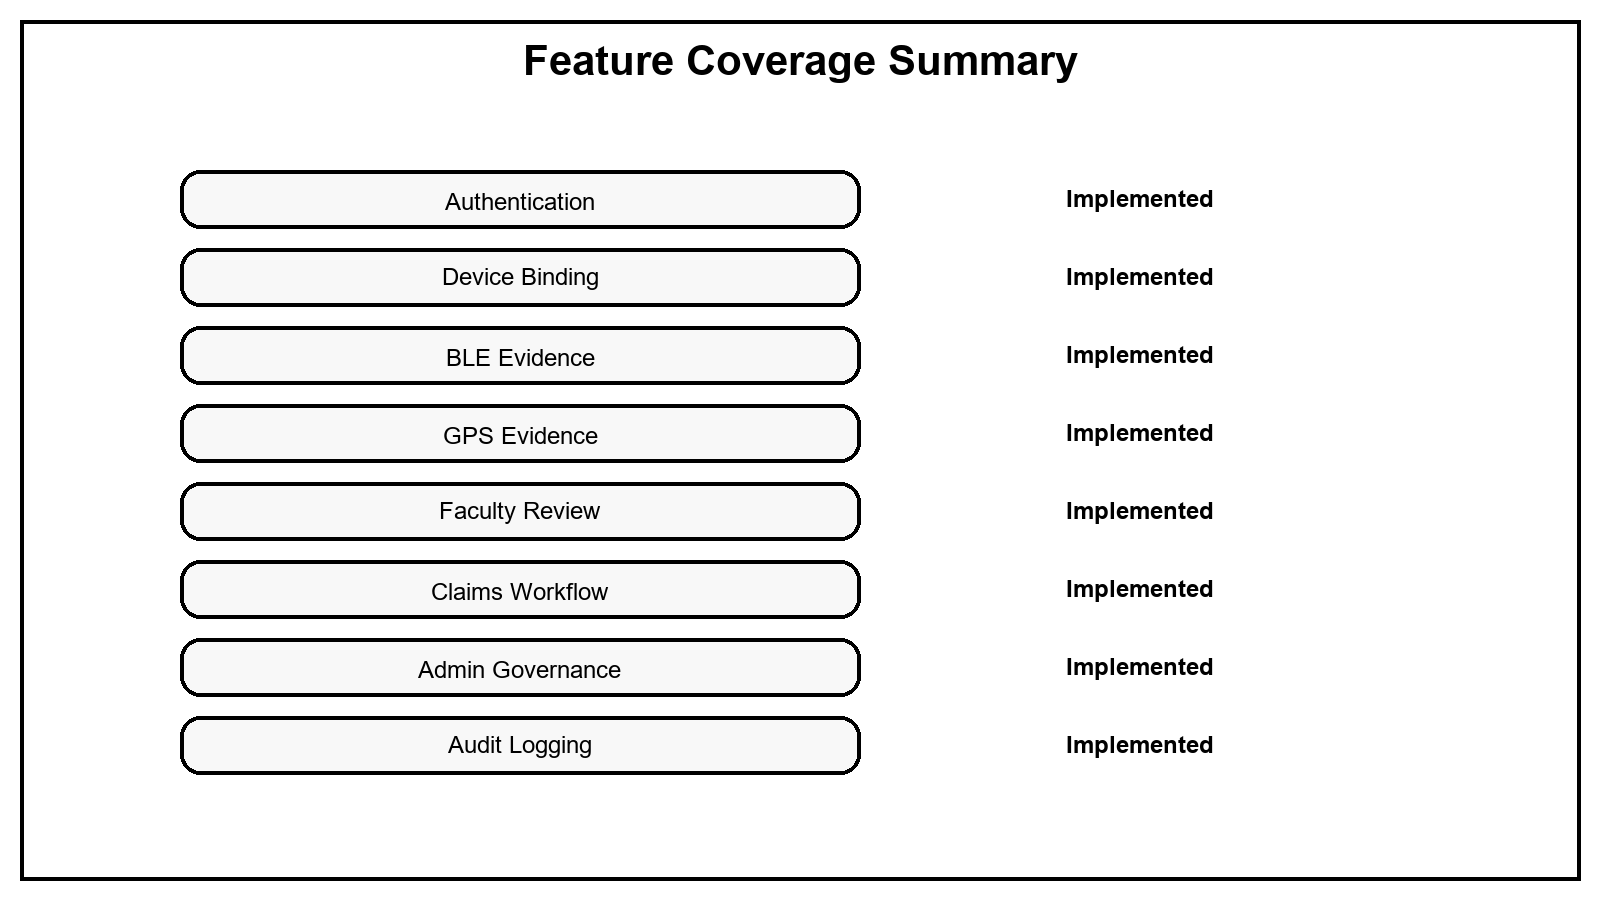
\includegraphics[width=0.8\textwidth]{images/fig8_1_feature_coverage.png}
    \caption{Comparative Feature Coverage}
    \label{fig:feature-coverage}
\end{figure}
% TODO: insert the comparative feature coverage chart at images/fig8_1_feature_coverage.png
% ASSUMPTION: this is a data chart, not a screenshot; no supplied image asset corresponds to it. The underlying
% data is fully tabulated in Table~8.7 (Table~\ref{tab:comparative-positioning}).
\section{Implemented System Footprint}

Table~\ref{tab:system-footprint} summarises the implemented footprint of HKS ATTENDANCE at the architectural level. The table focuses on structural characteristics of the delivered system --- supported roles, evidence channels, governance workflows, and core security controls --- rather than deployment-scale usage counts, since the project was evaluated primarily through controlled validation scenarios rather than long-running production operation.

\begin{table}[htbp]
\centering
\caption{Implemented System Footprint}
\label{tab:system-footprint}
\begin{tabularx}{\textwidth}{|l|X|}
\hline
\textbf{Aspect} & \textbf{Implemented Scope} \\
\hline
User Roles & Student, Faculty, Administrator \\
\hline
Attendance Evidence Channels & BLE proximity evidence and GPS geofence evidence \\
\hline
Attendance Outcomes & CONFIRMED, FLAGGED for faculty review, or blocked submission where mandatory preconditions fail \\
\hline
Faculty Governance & Review of flagged attendance, confirm/reject decisions, claim adjudication \\
\hline
Administrative Governance & User, course, enrolment, classroom, beacon, and device-binding management \\
\hline
Security Controls & JWT authentication, device binding, trusted beacon validation, nonce validation, replay protection, signature verification, audit logging \\
\hline
Persistence Layer & PostgreSQL relational database with normalised academic, attendance, claims, and security entities \\
\hline
Deployment Model & Mobile client + REST backend + database + classroom BLE beacon infrastructure \\
\hline
\end{tabularx}
\end{table}

\section{Major Contributions Restated}
\begin{itemize}
    \item A working hybrid BLE-and-GPS evidence-fusion architecture for attendance decisions.
    \item A one-student-one-device binding policy enforced at both the application and database level.
    \item A faculty governance workflow built around evidence inspection rather than fully automated decisioning.
    \item An administrative governance layer spanning the entire academic hierarchy and beacon estate.
    \item A claims and dispute-resolution workflow backed by a permanent audit trail.
\end{itemize}

\section{Project Achievements}

The following capabilities were designed, implemented, and verified as part of this project:

\begin{itemize}
    \item Complete Flutter application covering student, faculty, and administrator roles.
    \item FastAPI backend exposing a versioned, documented REST interface.
    \item PostgreSQL integration with a normalised, referentially consistent schema.
    \item JWT-based authentication with server-side session revocation.
    \item Device-binding enforcement preventing unauthorised credential sharing.
    \item BLE security hardening through nonce validation, freshness checks, and HMAC signature verification.
    \item Faculty governance workflow for reviewing and resolving ambiguous attendance records.
    \item Administrative governance covering the full academic hierarchy and BLE beacon estate.
    \item Claims and dispute-resolution workflow with permanent audit logging.
    \item Cloud deployment of the backend and database on a managed hosting platform.
    \item Integration with custom ESP32 beacon firmware for classroom proximity sensing.
\end{itemize}

\section{Limitations}
\begin{itemize}
    \item The system depends on ESP32 beacons being installed and correctly configured in each classroom where it is deployed.
    \item Attendance submission currently requires an active internet connection; no offline submission workflow has been implemented in this version.
    \item GPS readings remain variable indoors, which is why the architecture treats GPS as corroborating rather than decisive evidence.
    \item Testing to date has focused primarily on Android devices; broader device coverage would strengthen confidence in cross-platform behaviour.
\end{itemize}

\section{Chapter Summary}

This chapter assessed the outcomes of the project against its stated objectives via a consolidated achievement matrix, compared HKS ATTENDANCE to manual, BLE-only, and GPS-only alternatives, reported deployment statistics, restated the project's principal achievements, and acknowledged the limitations that remain. The final chapter concludes the thesis and outlines directions for future work.

% =============================================================================
% CHAPTER 9: CONCLUSION AND FUTURE WORK
% =============================================================================
\chapter{Conclusion and Future Work}
\label{chap:conclusion}

\section{Introduction}

This thesis addressed a problem that is easy to underestimate because attendance recording appears routine: nearly every widely used attendance technology, automated or otherwise, ultimately depends on a single point of failure. HKS ATTENDANCE was built to examine whether pairing two independently weak signals -- short-range BLE proximity and device GPS -- with device binding, faculty oversight, administrative governance, and a formal claims process, could produce a system that is meaningfully more resistant to impersonation, spoofing, and replay without becoming meaningfully harder to use.

\section{Summary of Work Completed}

The project proceeded through eight development phases. The first established a course-centric academic data model, replacing an earlier and more restrictive classroom-centric one. The second implemented enrolment-aware session discovery. The third -- and architecturally most significant -- built the hybrid BLE-and-GPS evidence layer, together with nonce validation, replay protection, timestamp freshness checks, and HMAC signature verification. The fourth delivered the complete student-facing experience. The fifth introduced faculty governance, giving human reviewers visibility into ambiguous attendance decisions. The sixth built out administrative governance across the academic hierarchy and beacon infrastructure. The seventh added the claims and appeals workflow. The eighth and final phase validated the complete system end to end, as documented in Chapter~7.

\section{Objectives Achieved}
\begin{itemize}
    \item A secure, multi-evidence attendance-collection platform was designed and implemented.
    \item Proxy attendance was substantially mitigated through device binding, BLE validation, and replay protection.
    \item Faculty governance was introduced, giving staff direct visibility into the evidence behind ambiguous decisions.
    \item Administrative governance was implemented across the full academic hierarchy and the beacon estate.
    \item A structured, auditable claims process now gives students a genuine path to contest disputed outcomes.
\end{itemize}

\section{Principal Contributions}
\begin{itemize}
    \item A hybrid BLE-and-GPS evidence-fusion model for attendance decisioning.
    \item A device-binding architecture enforcing a one-student-one-device policy.
    \item A faculty governance model that routes ambiguous cases to human review rather than resolving them automatically.
    \item A comprehensive administrative governance framework covering users, courses, enrolments, classrooms, beacons, and devices.
    \item A claims and appeals framework with permanent, auditable resolution records.
    \item An audit-driven design in which every consequential action leaves a traceable record.
\end{itemize}

\section{Security Achievements}

The implemented controls -- JWT authentication, device binding, nonce-based replay protection, timestamp freshness checks, HMAC signature verification, ownership validation for both faculty and claims actions, and comprehensive audit logging -- were each verified through the testing programme described in Chapter~7 and found to behave as designed, leaving the platform considerably more resistant to impersonation, spoofing, and replay attacks than the single-channel systems it was designed to improve upon.

\section{Practical Impact}

For students, the system offers visible, traceable attendance records and a genuine mechanism for appeal. For faculty, it offers evidence-based decision support, attendance analytics, and direct governance tools rather than unconditional trust in an automated verdict. For administrators, it offers centralised control over the academic structure and the device and beacon estate that underpins it. For the institution as a whole, the result is an improvement in attendance integrity, a reduction in the simplest forms of fraud, and a more complete audit trail than manual or single-channel systems provide.

\section{Limitations}
\begin{itemize}
    \item \textbf{Hardware dependency}: classrooms require a properly installed, registered ESP32 beacon to participate in BLE verification.
    \item \textbf{Connectivity dependency}: the current implementation has no offline attendance-capture path.
    \item \textbf{GPS variability}: indoor satellite positioning remains less reliable than its outdoor counterpart, which is why the architecture treats it as supporting rather than decisive evidence.
    \item \textbf{Device coverage}: validation to date has concentrated on Android devices available during development.
    \item \textbf{Single-institution evaluation}: the system has been evaluated within one academic environment; broader, multi-institution deployment remains future work.
\end{itemize}

\section{Future Work}

Future extensions to HKS ATTENDANCE are organised below into four groups: technical enhancements, security enhancements, user-experience improvements, and research extensions that go beyond incremental engineering.

\subsection{Technical Enhancements}
\begin{itemize}
    \item \textbf{Offline attendance capture} -- collecting and queuing evidence locally on a student's device when connectivity is unavailable, with deferred synchronisation and conflict resolution once a connection is restored.
    \item \textbf{Multi-campus deployment} -- the schema's normalisation around courses, classrooms, and beacons rather than a single fixed location should generalise reasonably well to centralised multi-campus management, though this has not yet been tested at that scale.
    \item \textbf{Cloud-native scaling} -- moving from a single containerised backend instance to a horizontally scaled deployment as institutional load grows, supported by the formal stress and load testing identified in Section~7.10 as not yet performed.
    \item \textbf{Integration with institutional systems} -- connecting to existing academic ERP platforms and learning-management systems so attendance data flows into the broader institutional record rather than remaining isolated.
\end{itemize}

\subsection{Security Enhancements}
\begin{itemize}
    \item \textbf{Certificate-based beacon authentication} -- replacing or supplementing the current shared-secret HMAC scheme with per-beacon certificates issued and rotated centrally.
    \item \textbf{Hardware-backed device attestation} -- using platform attestation APIs (where available) to strengthen device binding beyond a stored identifier.
    \item \textbf{Expanded anomaly detection on the audit log} -- flagging unusual patterns of faculty or administrative action for separate institutional review.
\end{itemize}

\subsection{User Experience}
\begin{itemize}
    \item \textbf{Real-time notifications} -- push notifications for attendance outcomes, claim updates, and session reminders, closing the feedback loop more quickly than the current pull-based history views.
    \item \textbf{Faculty analytics dashboard} -- attendance-trend analysis, early-warning risk indicators, and departmental-level reporting layered on top of the existing attendance and claims data without altering the underlying schema.
    \item \textbf{Web administration console} -- a browser-based administrative dashboard, alongside the existing mobile administrative tools, to ease bulk-management tasks for institutional staff working from a desktop.
\end{itemize}

\subsection{Research Extensions}
\begin{itemize}
    \item \textbf{Server-side BLE trilateration} -- rather than relying on a single beacon's RSSI reading, deploying multiple beacons per classroom and trilaterating the student device's position server-side would tighten spatial resolution further and provide an additional, independently computable evidence signal beyond simple proximity.
    \item \textbf{Machine-learning environmental calibration} -- learning per-classroom RSSI and GPS-accuracy baselines over time (rather than using fixed, institution-wide thresholds) so that the BLE and GPS validators automatically adapt to a room's specific radio and signal environment.
    \item \textbf{Ultra-wideband (UWB) indoor positioning} -- as UWB hardware becomes more common in smartphones, it offers room- and sub-room-level positioning precision that could supplement or eventually replace BLE proximity sensing.
    \item \textbf{Institutional federation} -- extending the device-binding and claims model to operate across multiple, independently administered institutions sharing infrastructure or courses.
    \item \textbf{Optional computer-vision head-count validation as a third evidence channel} -- the system can integrate a computer-vision module that captures a classroom image at the start or end of a session and performs head counting using an object-detection model. The detected number of students present can then be compared against the total number of attendance submissions recorded as CONFIRMED or FLAGGED for that session. Any material discrepancy between the two counts can automatically alert the responsible faculty member, providing an additional, independent evidence layer that operates above the level of any individual student's submission rather than replacing the existing BLE/GPS evidence for that student. This extension is explored cautiously, given the cost, accuracy, and privacy considerations discussed in Chapter~2, and is intended as an opt-in, classroom-level corroborating signal rather than a replacement for BLE or GPS evidence at the individual level.
    \item \textbf{Smartwatch BLE verification} -- extending proximity evidence collection to wearable devices, which may reduce reliance on a student actively operating a phone during the verification window.
    \item \textbf{Machine-learning anomaly detection on submitted evidence} -- learning typical patterns of BLE signal strength and GPS accuracy per classroom over time, to flag evidence that is statistically unusual even when it passes the deterministic checks described in Chapter~4.
\end{itemize}

\section{Final Remarks}

HKS ATTENDANCE demonstrates that pairing two individually imperfect signals -- Bluetooth proximity and satellite-derived location -- with device binding, human governance, and a formal appeals process can produce an attendance platform that is considerably more resistant to impersonation, spoofing, and replay than the single-channel alternatives still in widespread use, without imposing a significantly heavier burden on the students and staff who use it day to day. The project met the objectives set out at its inception and provides a practical foundation that could be extended toward institution-wide deployment.

% =============================================================================
% REFERENCES / BIBLIOGRAPHY
% =============================================================================
\addcontentsline{toc}{chapter}{References}

\begin{thebibliography}{99}

\bibitem{ref1} S. A. Ahson and M. Ilyas, ``Bluetooth-Based Attendance Management System,'' \textit{International Journal of Computer Applications}, vol. 97, no. 14, pp. 15--21, 2019.

\bibitem{ref2} R. Gupta and P. Sharma, ``Smart Attendance Monitoring Using BLE Technology,'' \textit{Proc. International Conference on Emerging Technologies}, pp. 112--118, 2020.

\bibitem{ref3} M. N. Hossain, M. A. Rahman, and S. K. Das, ``Location-Based Attendance Using GPS and Mobile Devices,'' \textit{Proc. IEEE International Conference on Smart Computing}, pp. 235--241, 2018.

\bibitem{ref4} K. Chawla, A. Singh, and V. Kumar, ``Secure Attendance Management Using Multi-Factor Verification,'' \textit{International Journal of Advanced Computer Science and Applications}, vol. 11, no. 6, 2020.

\bibitem{ref5} P. Gupta and R. Arora, ``A Survey of Attendance-Monitoring Systems Using Wireless Technologies,'' \textit{International Journal of Scientific Research in Computer Science}, vol. 9, no. 4, 2021.

\bibitem{ref6} Bluetooth SIG, \textit{Bluetooth Core Specification Version 5.3}, 2021.

\bibitem{ref7} Espressif Systems, \textit{ESP32 Technical Reference Manual}, 2024.

\bibitem{ref8} Espressif Systems, \textit{ESP-IDF Programming Guide}.

\bibitem{ref9} N. Golmie, R. E. Van Dyck, and A. Soltanian, ``Interference of Bluetooth and IEEE 802.11: Simulation Modeling and Performance Evaluation,'' \textit{IEEE Wireless Communications}, vol. 10, no. 6, pp. 22--29, 2003.

\bibitem{ref10} Google Developers, \textit{Android Location Services Documentation}.

\bibitem{ref11} \textit{Geolocator Package Documentation}, pub.dev.

\bibitem{ref12} B. Hofmann-Wellenhof, H. Lichtenegger, and E. Wasle, \textit{GNSS -- Global Navigation Satellite Systems}, Springer, 2008.

\bibitem{ref13} B. Schneier, \textit{Applied Cryptography: Protocols, Algorithms and Source Code in C}, 2nd ed., Wiley, 1996.

\bibitem{ref14} W. Stallings, \textit{Cryptography and Network Security}, 7th ed., Pearson Education, 2017.

\bibitem{ref15} OWASP Foundation, \textit{OWASP API Security Top 10}.

\bibitem{ref16} RFC 2104, \textit{HMAC: Keyed-Hashing for Message Authentication}, IETF.

\bibitem{ref17} RFC 7519, \textit{JSON Web Token (JWT)}, IETF.

\bibitem{ref18} PostgreSQL Global Development Group, \textit{PostgreSQL Documentation}.

\bibitem{ref19} R. Elmasri and S. Navathe, \textit{Fundamentals of Database Systems}, 7th ed., Pearson, 2016.

\bibitem{ref20} C. J. Date, \textit{An Introduction to Database Systems}, 8th ed., Pearson, 2003.

\bibitem{ref21} \textit{FastAPI Documentation}, fastapi.tiangolo.com.

\bibitem{ref22} \textit{SQLAlchemy Documentation}, sqlalchemy.org.

\bibitem{ref23} \textit{Alembic Documentation}, alembic.sqlalchemy.org.

\bibitem{ref24} \textit{Pydantic Documentation}, docs.pydantic.dev.

\bibitem{ref25} \textit{Flutter Documentation}, flutter.dev.

\bibitem{ref26} \textit{Flutter Blue Plus Documentation}, pub.dev.

\bibitem{ref27} \textit{Riverpod Documentation}, riverpod.dev.

\bibitem{ref28} \textit{Dio HTTP Client Documentation}, pub.dev.

\bibitem{ref29} I. Sommerville, \textit{Software Engineering}, 10th ed., Pearson Education, 2015.

\bibitem{ref30} R. S. Pressman, \textit{Software Engineering: A Practitioner's Approach}, 8th ed., McGraw Hill, 2014.

\bibitem{ref31} M. Fowler, \textit{Patterns of Enterprise Application Architecture}, Addison-Wesley, 2002.

\bibitem{ref32} S. Patil and V. Patil, ``Smart Attendance System Using BLE Beacons and Mobile Applications,'' \textit{International Journal of Innovative Research in Computer Science}, 2021.

\bibitem{ref33} A. Khan, S. Ahmed, and M. Hussain, ``IoT-Based Smart Attendance Monitoring Framework,'' \textit{Proc. IEEE International Conference on Internet of Things}, 2019.

\bibitem{ref34} J. Wang and H. Li, ``Hybrid Attendance Verification Using Wireless Technologies,'' \textit{Journal of Wireless Communications}, vol. 12, no. 3, 2020.

\bibitem{ref35} All India Council for Technical Education (AICTE), \textit{Project Guidelines for Undergraduate Engineering Programs}.

\bibitem{ref36} Indian Institute of Information Technology Raichur, \textit{Academic Regulations and Major Project Guidelines}, Academic Year 2025-26.

\bibitem{ref37} \textit{Swagger / OpenAPI Specification}, swagger.io.

\bibitem{ref38} F. Adib and D. Katabi, ``See Through Walls with Wi-Fi!,'' \textit{Proc. ACM SIGCOMM}, pp. 75--86, 2013.

\bibitem{ref39} A. Bensky, \textit{Wireless Positioning Technologies and Applications}, 2nd ed., Artech House, 2016.

\bibitem{ref40} S. Gezici et al., ``Localization via Ultra-Wideband Radios,'' \textit{IEEE Signal Processing Magazine}, vol. 22, no. 4, pp. 70--84, 2005.

\bibitem{ref41} Y. Zhuang, J. Yang, Y. Li, L. Qi, and N. El-Sheimy, ``Smartphone-Based Indoor Localization with Bluetooth Low Energy Beacons,'' \textit{Sensors}, vol. 16, no. 5, 2016.

\bibitem{ref42} M. S. Hossain and A. F. Hossain, ``A Survey on Bluetooth Low Energy Based Indoor Positioning,'' \textit{Proc. IEEE International Conference on Computing}, 2019.

\bibitem{ref43} J. Viterbo et al., ``RSSI-Based Indoor Positioning Using BLE Beacons,'' \textit{Proc. International Conference on Indoor Positioning and Indoor Navigation (IPIN)}, 2018.

\bibitem{ref44} A. Yassin et al., ``Recent Advances in Indoor Localization: A Survey on Theoretical Approaches and Applications,'' \textit{IEEE Communications Surveys \& Tutorials}, vol. 19, no. 2, pp. 1327--1346, 2017.

\bibitem{ref45} L. Mainetti, L. Patrono, and I. Sergi, ``A Survey on Indoor Positioning Systems,'' \textit{Proc. International Conference on Software, Telecommunications and Computer Networks}, 2014.

\bibitem{ref46} K. He, X. Zhang, S. Ren, and J. Sun, ``Deep Residual Learning for Image Recognition,'' \textit{Proc. IEEE Conference on Computer Vision and Pattern Recognition (CVPR)}, pp. 770--778, 2016.

\bibitem{ref47} J. Redmon and A. Farhadi, ``YOLOv3: An Incremental Improvement,'' \textit{arXiv preprint arXiv:1804.02767}, 2018.

\bibitem{ref48} S. Ren, K. He, R. Girshick, and J. Sun, ``Faster R-CNN: Towards Real-Time Object Detection with Region Proposal Networks,'' \textit{IEEE Transactions on Pattern Analysis and Machine Intelligence}, vol. 39, no. 6, pp. 1137--1149, 2017.

\bibitem{ref49} F. Schroff, D. Kalenichenko, and J. Philbin, ``FaceNet: A Unified Embedding for Face Recognition and Clustering,'' \textit{Proc. IEEE CVPR}, pp. 815--823, 2015.

\bibitem{ref50} European Parliament and Council, \textit{General Data Protection Regulation (GDPR)}, Regulation (EU) 2016/679.

\bibitem{ref51} Government of India, \textit{Digital Personal Data Protection Act}, 2023.

\bibitem{ref52} N. Provos and D. Mazi\`{e}res, ``A Future-Adaptable Password Scheme,'' \textit{Proc. USENIX Annual Technical Conference}, 1999.

\bibitem{ref53} D. Eastlake and P. Jones, RFC 3174, \textit{US Secure Hash Algorithm 1 (SHA1)}, IETF, 2001.

\bibitem{ref54} M. Bellare, R. Canetti, and H. Krawczyk, ``Keying Hash Functions for Message Authentication,'' \textit{Proc. CRYPTO}, pp. 1--15, 1996.

\bibitem{ref55} Internet Engineering Task Force (IETF), RFC 6749, \textit{The OAuth 2.0 Authorization Framework}.

\bibitem{ref56} Google Developers, \textit{Fused Location Provider API Documentation}.

\bibitem{ref57} Docker Inc., \textit{Docker Documentation}, docs.docker.com.

\bibitem{ref58} Railway Corp., \textit{Railway Platform Documentation}, docs.railway.app.

\bibitem{ref59} M. Richardson and S. Ruby, \textit{RESTful Web Services}, O'Reilly Media, 2007.

\bibitem{ref60} R. T. Fielding, \textit{Architectural Styles and the Design of Network-Based Software Architectures}, PhD Dissertation, University of California, Irvine, 2000.

\end{thebibliography}

% =============================================================================
% PUBLICATIONS
% =============================================================================
\chapter*{Publications Arising From This Work}
\addcontentsline{toc}{chapter}{Publications Arising From This Work}

At the time of submission, no peer-reviewed publication has been produced from this work. The author intends to extend the system and prepare a research manuscript based on the multi-evidence attendance architecture presented in this thesis.

% =============================================================================
% APPENDICES
% =============================================================================
\appendix

\chapter{Selected API Endpoints}
\label{app:api-endpoints}

A representative subset of the REST API exposed by the backend is summarised below; the full interface (60+ endpoints across 18 router modules, per Table~5.5) is documented through the project's Swagger UI.

\begin{table}[htbp]
\centering
\caption{Representative API Endpoints}
\label{tab:api-endpoints}
\begin{tabularx}{\textwidth}{|l|X|}
\hline
\textbf{Endpoint} & \textbf{Purpose} \\
\hline
POST /auth/login & Authenticate a user and issue a JWT \\
\hline
POST /auth/logout & Revoke the active session \\
\hline
GET /sessions/my-active-sessions & List active sessions for an enrolled student \\
\hline
POST /sessions/start & Faculty: start a new attendance session \\
\hline
POST /sessions/\{id\}/close & Faculty: close an active session \\
\hline
POST /attendance/submit & Submit BLE and GPS evidence for attendance \\
\hline
GET /attendance/my-history & Retrieve a student's attendance history \\
\hline
GET /faculty/flagged-attendance & List attendance records awaiting review \\
\hline
POST /faculty/attendance/\{id\}/confirm & Confirm a flagged attendance record \\
\hline
POST /faculty/attendance/\{id\}/reject & Reject a flagged attendance record \\
\hline
POST /claims & Submit a claim against rejected attendance \\
\hline
POST /faculty/claims/\{id\}/approve & Approve a student claim \\
\hline
POST /faculty/claims/\{id\}/reject & Reject a student claim \\
\hline
POST /admin/device/unbind & Administrator: unbind a registered device \\
\hline
\end{tabularx}
\end{table}

\chapter{Database Table Summary}
\label{app:db-tables}

\begin{table}[htbp]
\centering
\caption{Principal Database Tables}
\label{tab:db-tables}
\begin{tabularx}{\textwidth}{|l|X|}
\hline
\textbf{Table} & \textbf{Purpose} \\
\hline
users & Stores student, faculty, and administrator accounts \\
\hline
devices & Stores the device bound to each student account \\
\hline
auth\_sessions & Tracks active authentication sessions for revocation \\
\hline
courses & Stores the academic course catalogue \\
\hline
faculty\_courses & Maps faculty members to the courses they own \\
\hline
enrollments & Maps students to the courses they are enrolled in \\
\hline
classrooms & Stores classroom coordinates and geofence radius \\
\hline
trusted\_ble\_beacons & Registers beacon identifiers as trusted per classroom \\
\hline
beacon\_secrets & Stores the cryptographic key for each beacon's signature \\
\hline
attendance\_sessions & Represents an attendance window for a course/classroom \\
\hline
attendance & Stores the core attendance record for each submission, including the student, session, attendance status, and links to the associated BLE and GPS evidence \\
\hline
attendance\_ble\_evidence & Stores BLE evidence for an attendance attempt \\
\hline
attendance\_gps\_evidence & Stores GPS evidence for an attendance attempt \\
\hline
attendance\_claims & Stores student appeals against rejected attendance \\
\hline
faculty\_action\_logs & Permanent audit trail of faculty governance decisions \\
\hline
ble\_nonce\_cache & Stores previously used nonces for replay protection \\
\hline
\end{tabularx}
\end{table}

\chapter{Selected Viva-Voce Questions and Answers}
\label{app:viva}

\noindent\textbf{Q1. What problem does HKS ATTENDANCE solve?}

It addresses the single-point-of-failure weakness shared by most existing attendance technologies -- proxy attendance, unverifiable location claims, and the absence of any structured dispute process -- by combining BLE proximity evidence, GPS geofence evidence, device binding, faculty review, and a formal claims workflow into one platform.

\noindent\textbf{Q2. Why combine BLE and GPS rather than using either alone?}

BLE confirms short-range proximity to a specific classroom but says nothing about a device's broader location or absolute identity; GPS confirms approximate location but degrades indoors and can be falsified. Used together, an attacker must defeat both independently, which is considerably harder than defeating either alone.

\noindent\textbf{Q3. Why was the project not built around QR codes or RFID cards?}

Both were considered and explicitly set aside during the literature review in Chapter~2. A scannable code can be photographed and forwarded to someone who is not physically present, and an RFID card can simply be lent to a classmate; neither weakness is solved by adding more code or more cards. BLE proximity combined with GPS and device binding addresses the same underlying problem -- proving genuine physical presence -- without inheriting either of those specific failure modes.

\noindent\textbf{Q4. How is replay protection implemented?}

Each beacon broadcast carries a single-use nonce. Once the backend has accepted a nonce, it is stored in the BLE nonce cache, and any later attempt to submit a payload containing that same nonce is rejected outright.

\noindent\textbf{Q5. What happens when BLE and GPS evidence disagree?}

The record is marked FLAGGED rather than being automatically accepted or rejected, and is routed to the faculty member responsible for the session for manual evidence review.

\noindent\textbf{Q6. How is device binding enforced?}

A student's first successful login registers their device's unique identifier against their account. Every subsequent attendance submission is checked against this stored identifier; a request from any other device is rejected. An administrator must explicitly unbind a device before a student can register a replacement.

\noindent\textbf{Q7. What can a student do if their attendance is rejected unfairly?}

They can open a claim explaining why they believe the rejection was incorrect. The faculty member who owns the course reviews the claim and either approves it, which restores the record to CONFIRMED, or rejects it, leaving the original outcome in place. Either way, the decision is permanently logged.

\noindent\textbf{Q8. Why was PostgreSQL chosen over a non-relational database?}

The data model is inherently relational -- students, courses, sessions, evidence, and claims all reference one another -- and PostgreSQL's strong foreign-key enforcement and ACID guarantees make it well-suited to preserving that structure reliably.

\noindent\textbf{Q9. What are the main limitations of the current system?}

It requires properly installed BLE beacons in every participating classroom, requires an active internet connection at submission time, inherits GPS's known indoor-accuracy limitations (mitigated by treating GPS as corroborating rather than decisive), and has so far been validated primarily on Android devices within a single institution.

\noindent\textbf{Q10. What would be the next priority for future development?}

Offline evidence capture with deferred synchronisation would likely deliver the largest practical improvement, since the current reliance on live connectivity is the constraint most likely to affect day-to-day deployment.

\noindent\textbf{Q11. How would a computer-vision head-count check fit into the existing architecture?}

It would operate as a session-level, classroom-wide corroborating signal rather than a per-student evidence channel: a camera image captured at the start or end of a session would be passed through an object-detection model to estimate the number of students present, and that count would be compared against the number of CONFIRMED/FLAGGED attendance attempts for the session, with a material mismatch raised to the faculty member as an alert rather than used to alter any individual student's recorded status.

\noindent\textbf{Q12. Is the system "cheat-proof"?}

No system can be claimed to be entirely cheat-proof; the more accurate claim, and the one this thesis makes, is that combining two independent evidence channels with device binding and faculty review makes HKS ATTENDANCE considerably more resistant to impersonation, spoofing, and replay than the single-channel systems it was designed to improve upon.

% =========================
% APPENDIX SCREENSHOTS TEMPORARILY DISABLED FOR COMPILE STABILITY
% Uncomment later once final PDF is stable or when using a paid plan / local compile.
% =========================
\iffalse
\chapter{Application Screenshots}
\label{app:screenshots}

This appendix presents the application screenshots captured from the running system, organised by role/module and grouped to match the folder structure of the accompanying \texttt{images/screenshots/} directory. These screenshots correspond directly to the in-text figure placeholders referenced throughout Chapter~6 (Figures 6.1--6.7) and provide additional, appendix-only evidence beyond the single representative screenshot shown per module in the main chapter.

\section{Admin Screenshots}
\label{app:screenshots-admin}

\begin{figure}[htbp]
    \centering
    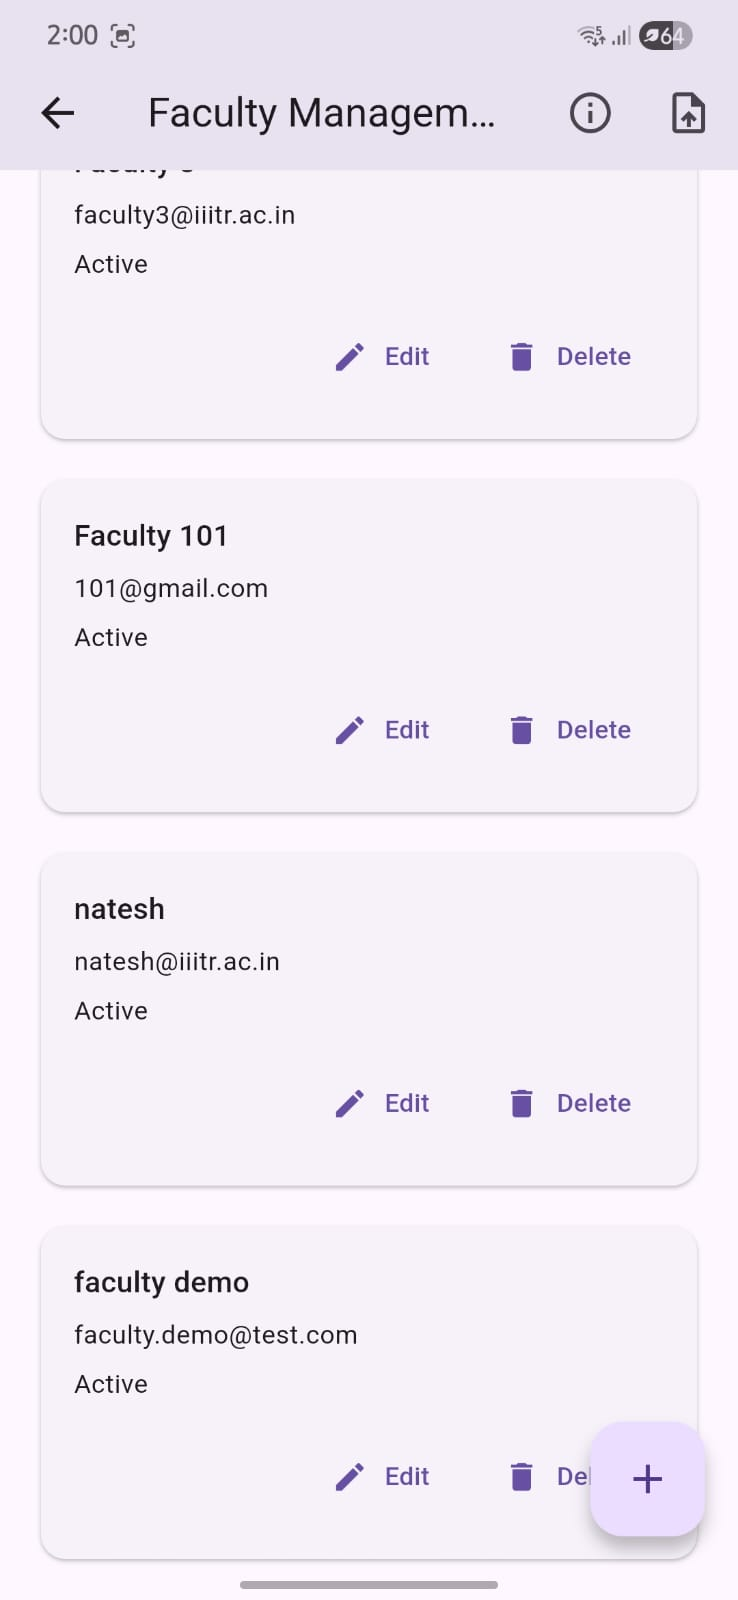
\includegraphics[width=0.48\textwidth]{images/screenshots/admin/ADM_01_create_faculty_01.jpeg}
    \hfill
    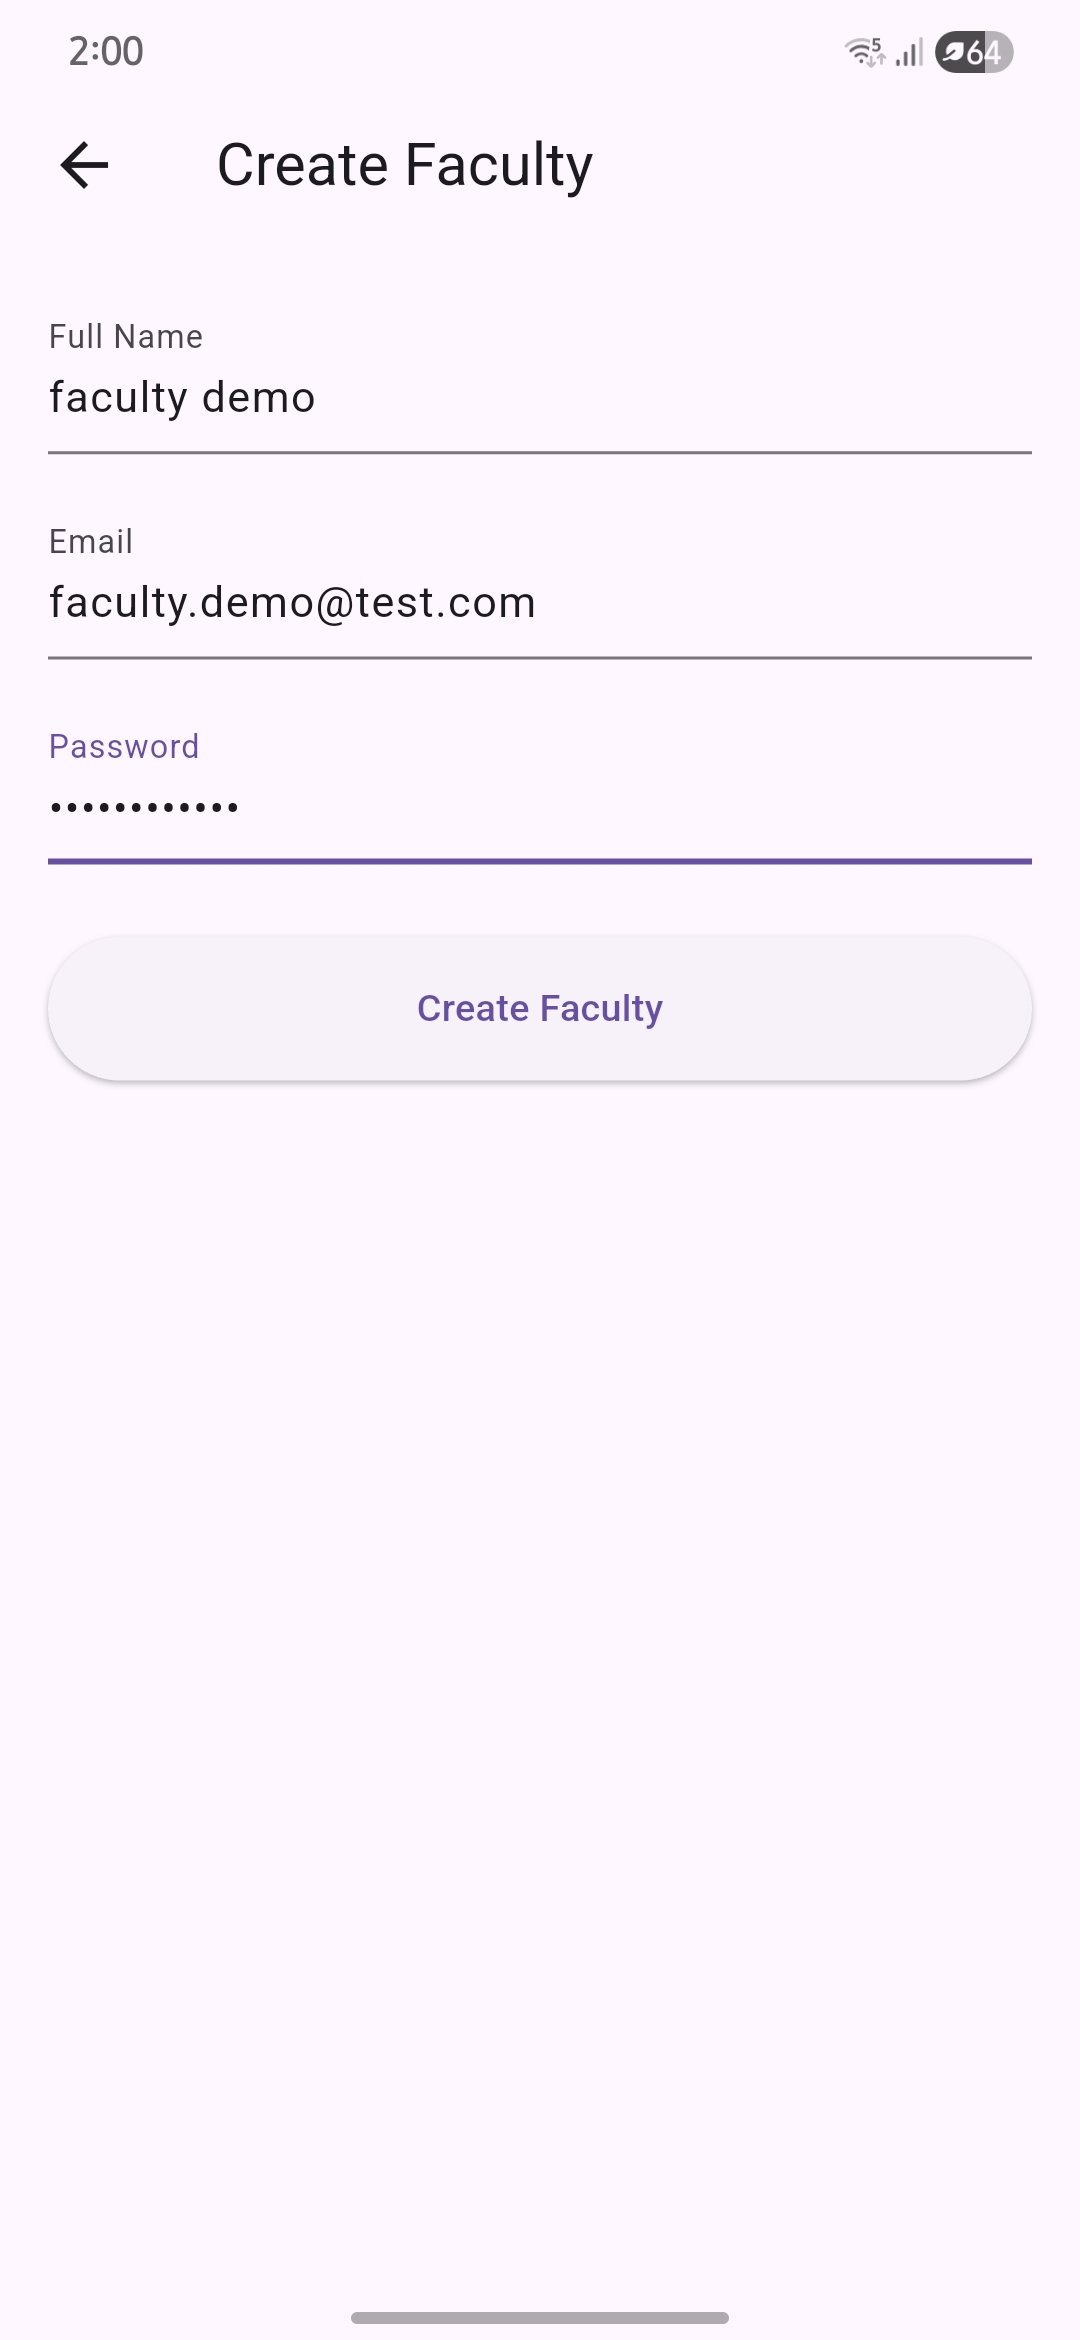
\includegraphics[width=0.48\textwidth]{images/screenshots/admin/ADM_01_create_faculty_02.jpeg}
    \caption{Admin: Create Faculty (Step 1 and Step 2)}
    \label{fig:appD-adm-01}
\end{figure}

\begin{figure}[htbp]
    \centering
    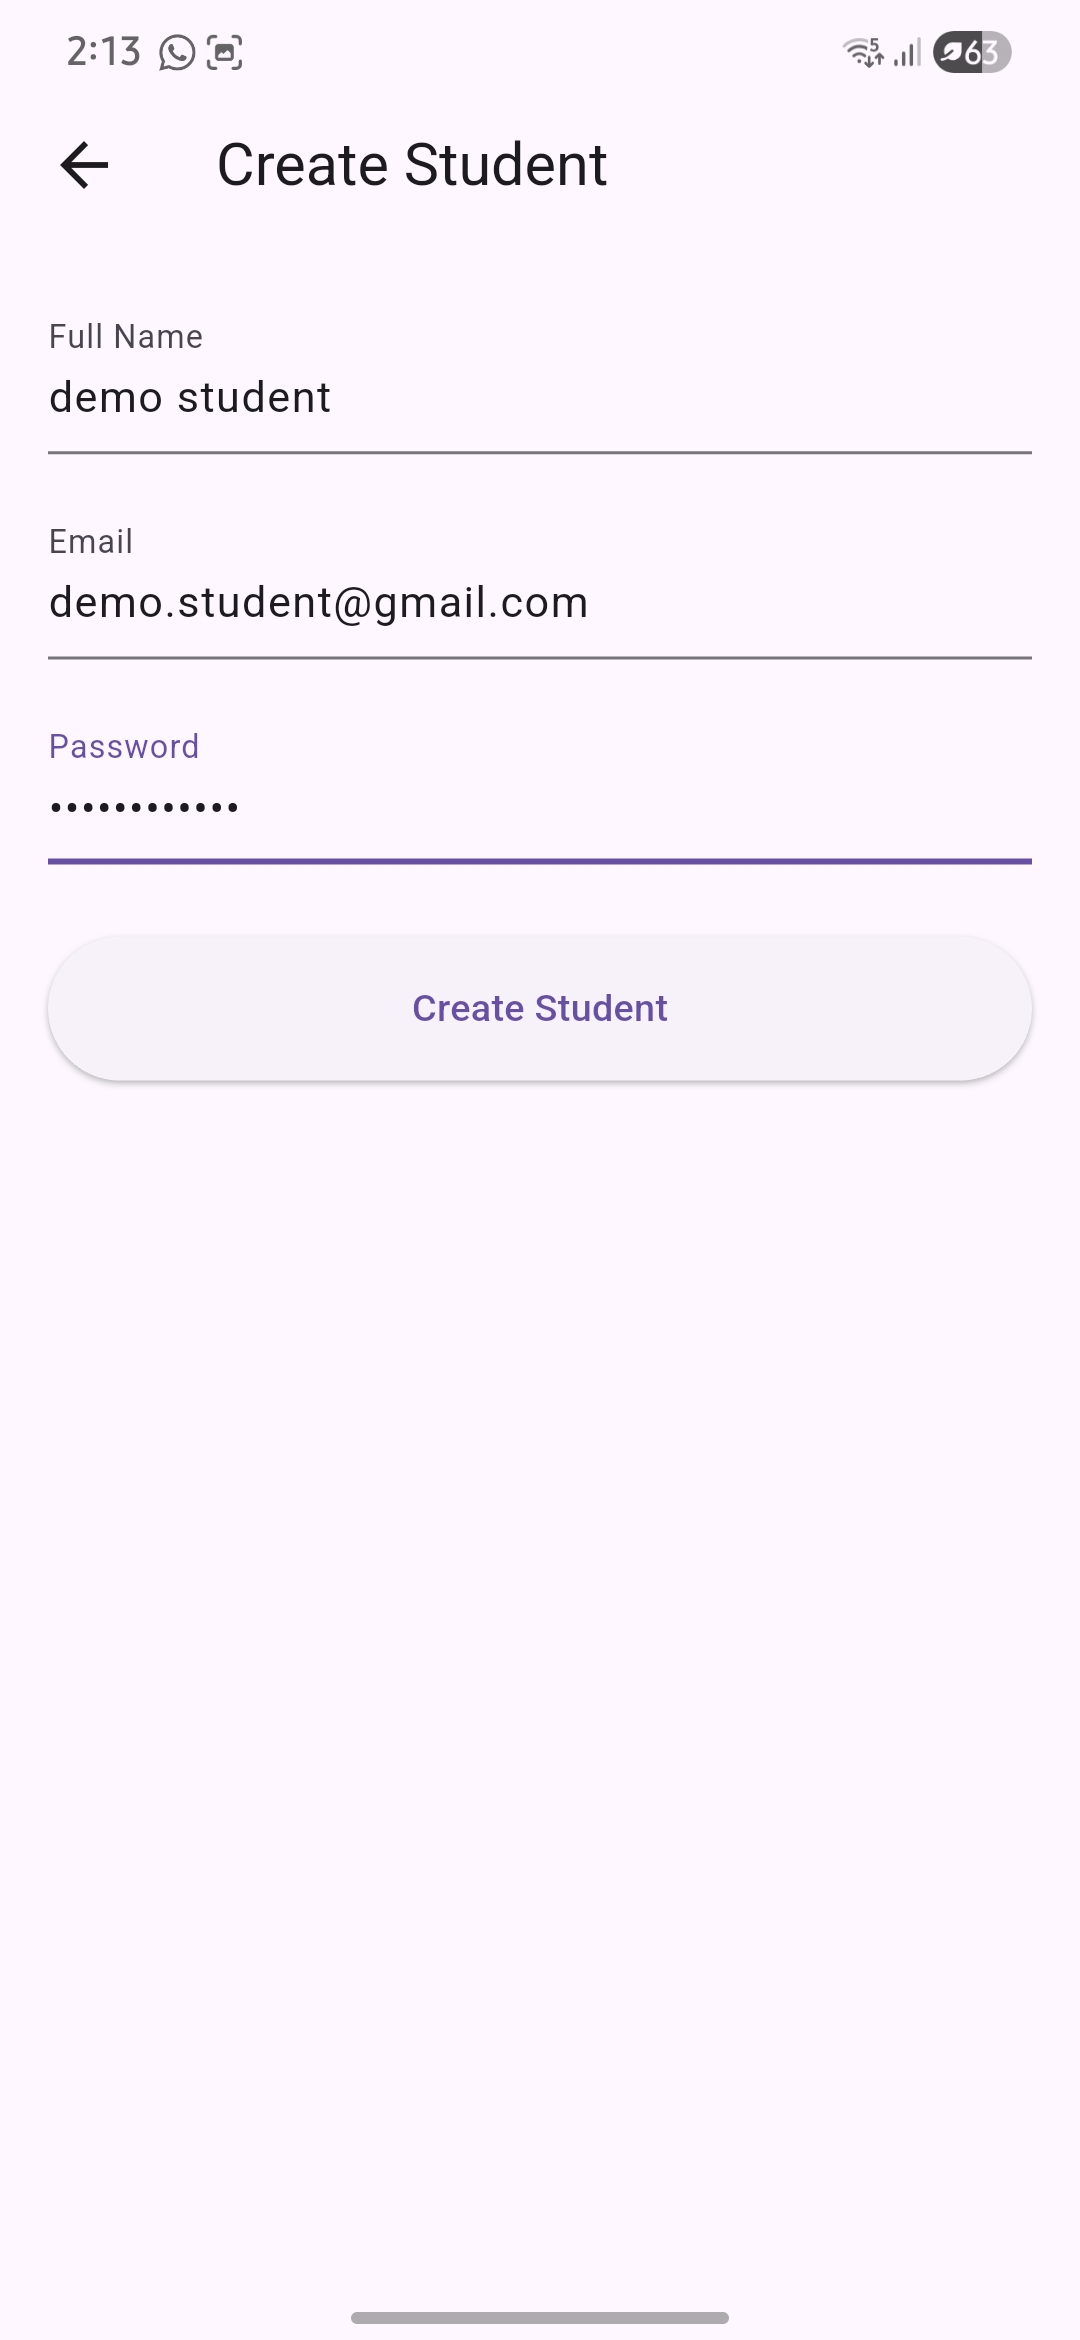
\includegraphics[width=0.48\textwidth]{images/screenshots/admin/ADM_02_create_student_01.jpeg}
    \hfill
    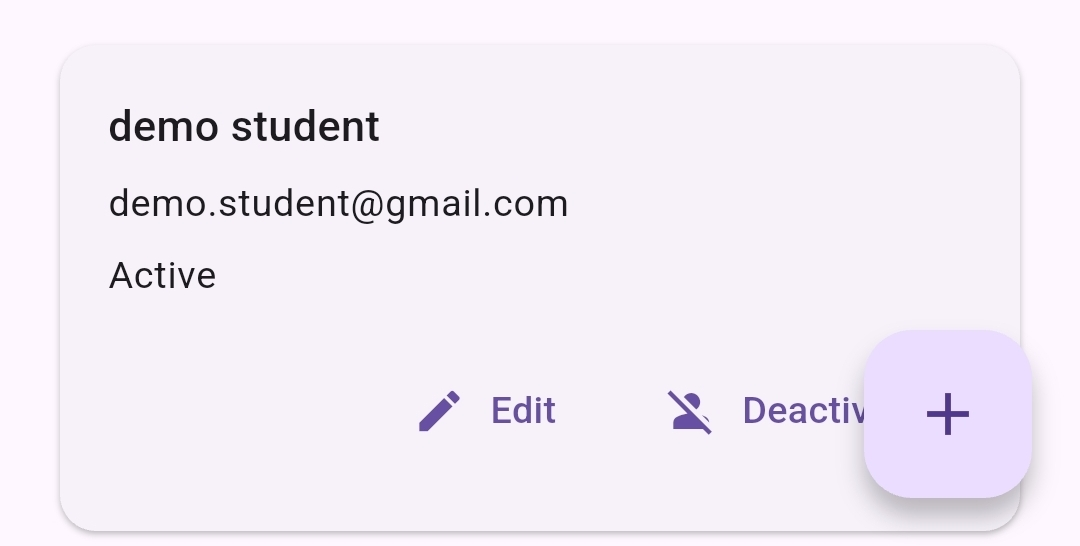
\includegraphics[width=0.48\textwidth]{images/screenshots/admin/ADM_02_create_student_02.jpeg}
    \caption{Admin: Create Student (Step 1 and Step 2)}
    \label{fig:appD-adm-02}
\end{figure}

\begin{figure}[htbp]
    \centering
    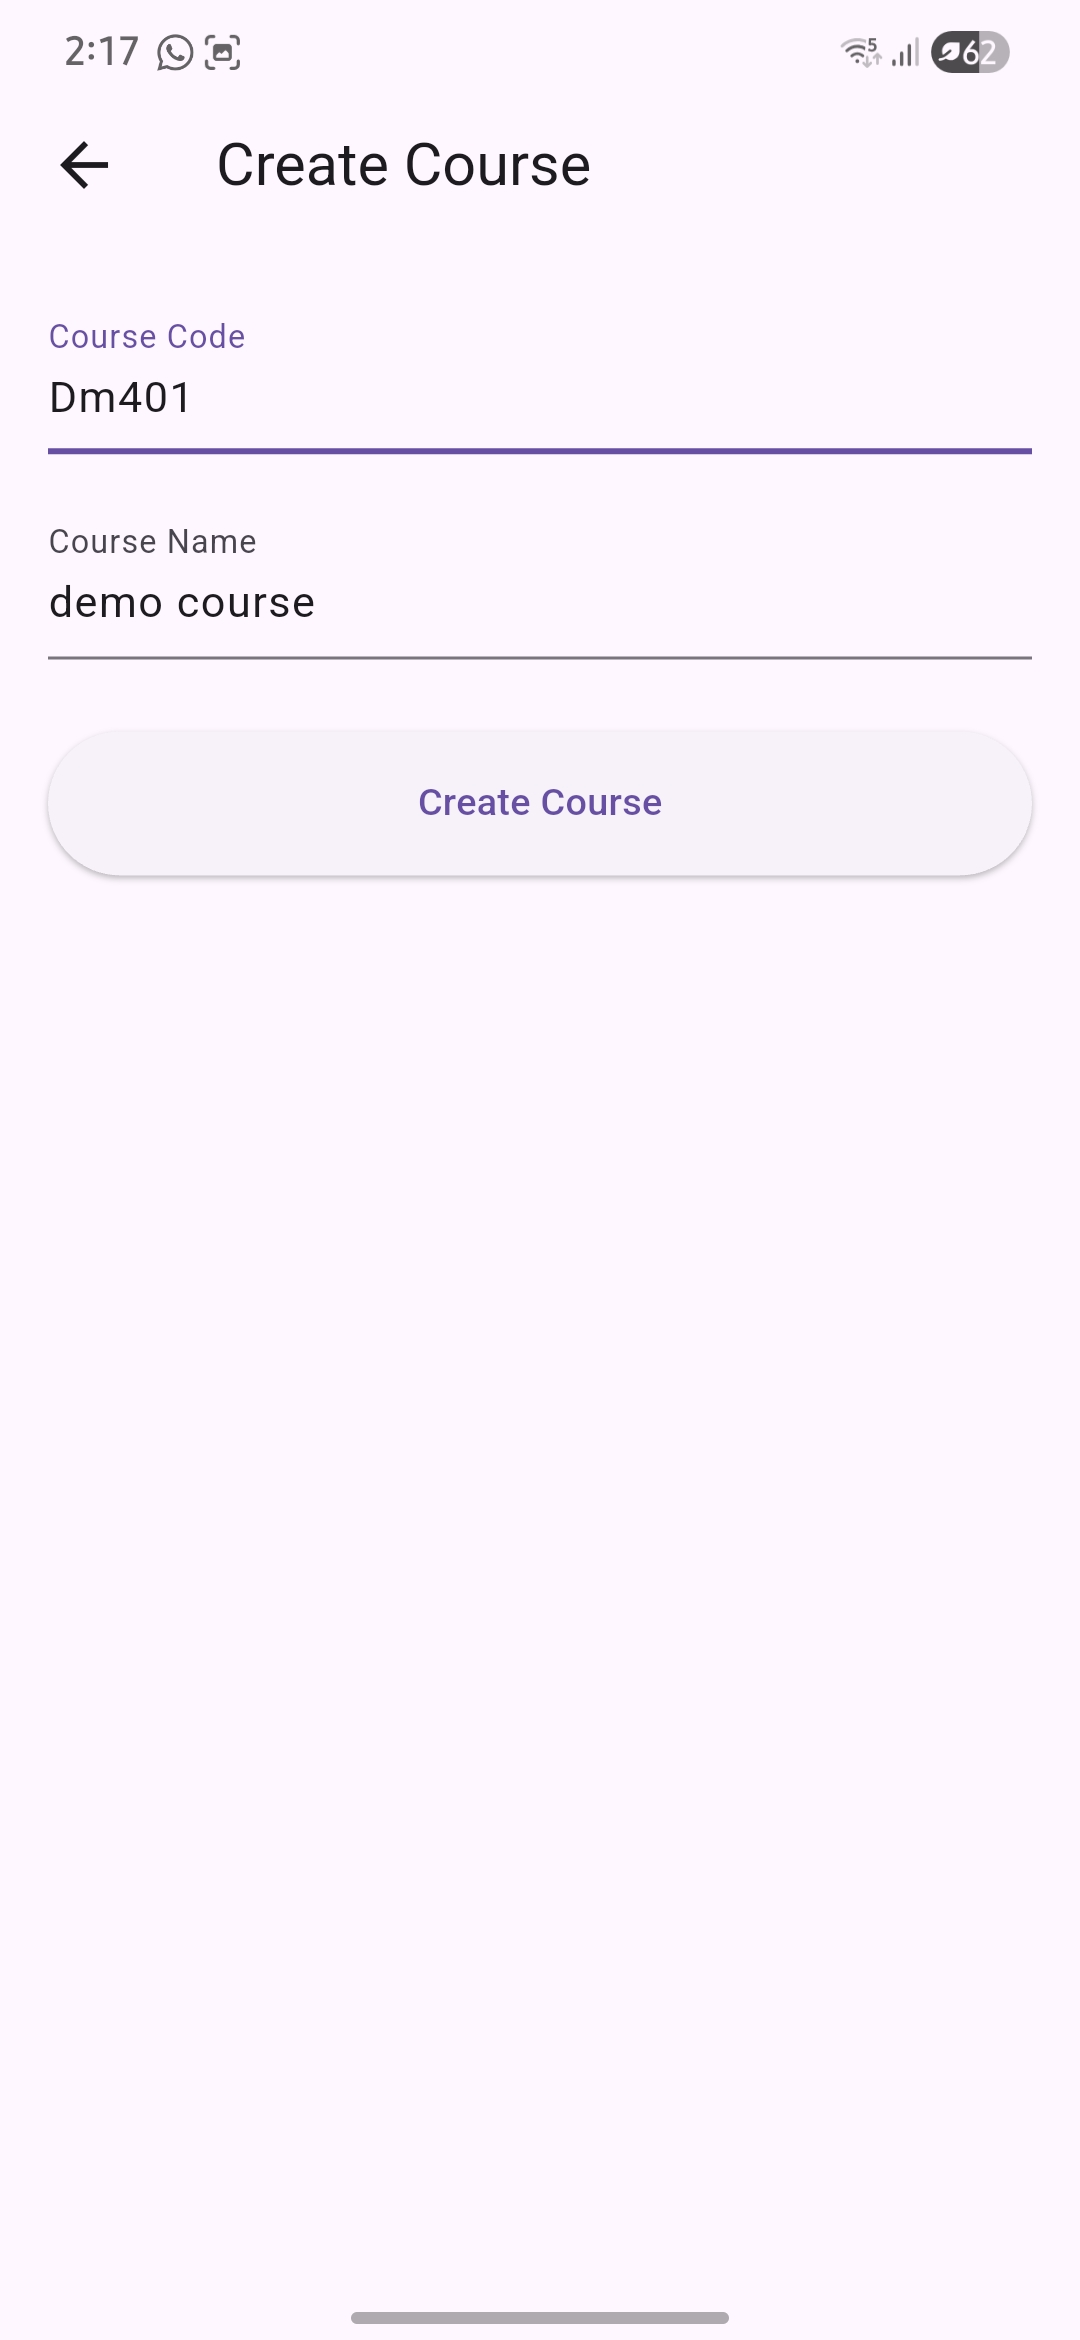
\includegraphics[width=0.48\textwidth]{images/screenshots/admin/ADM_03_create_course_01.jpeg}
    \hfill
    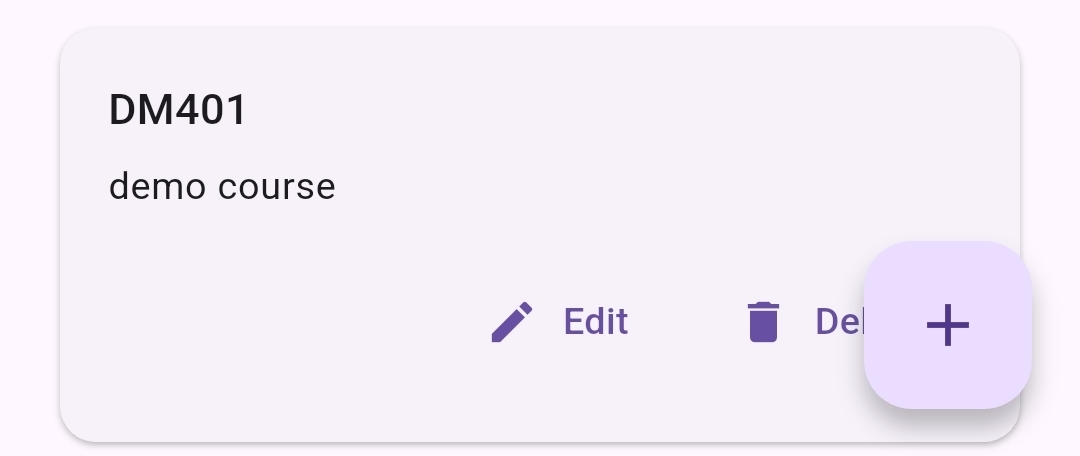
\includegraphics[width=0.48\textwidth]{images/screenshots/admin/ADM_03_create_course_02.jpeg}
    \caption{Admin: Create Course (Step 1 and Step 2)}
    \label{fig:appD-adm-03}
\end{figure}

\begin{figure}[htbp]
    \centering
    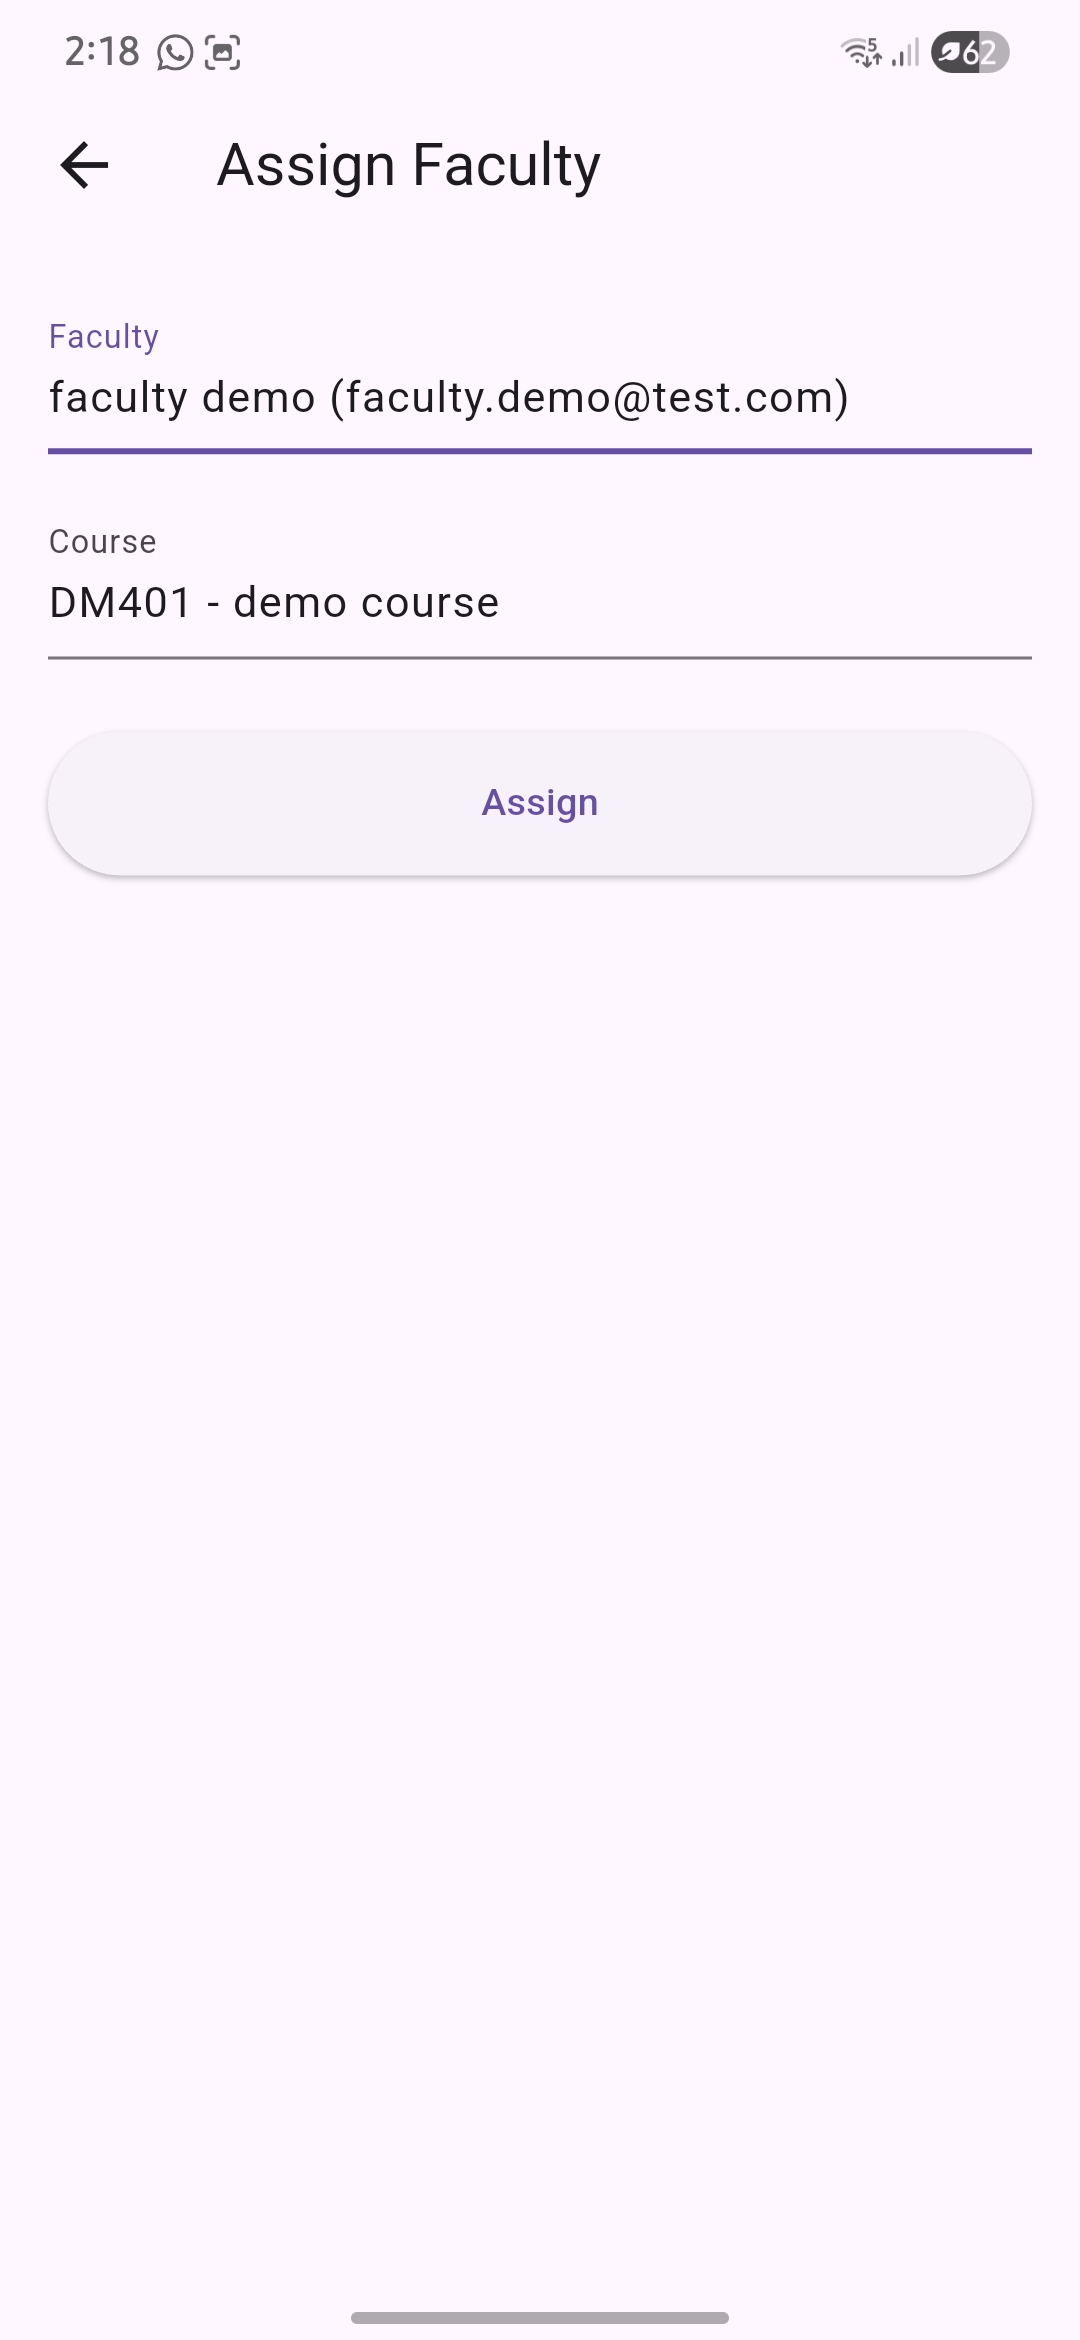
\includegraphics[width=0.48\textwidth]{images/screenshots/admin/ADM_04_assign_faculty_01.jpeg}
    \hfill
    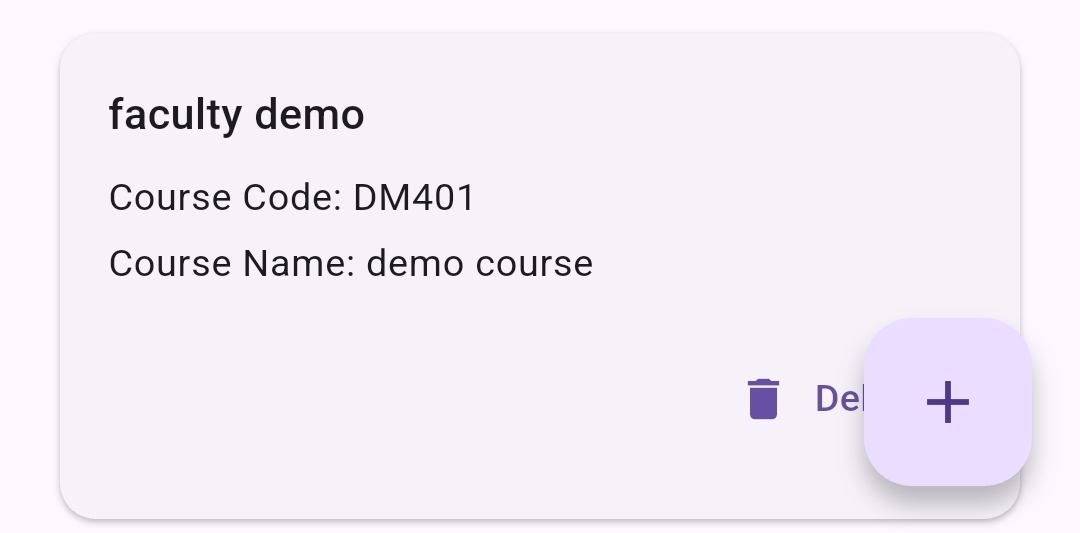
\includegraphics[width=0.48\textwidth]{images/screenshots/admin/ADM_04_assign_faculty_02.jpeg}
    \caption{Admin: Assign Faculty to Course (Step 1 and Step 2)}
    \label{fig:appD-adm-04}
\end{figure}

\begin{figure}[htbp]
    \centering
    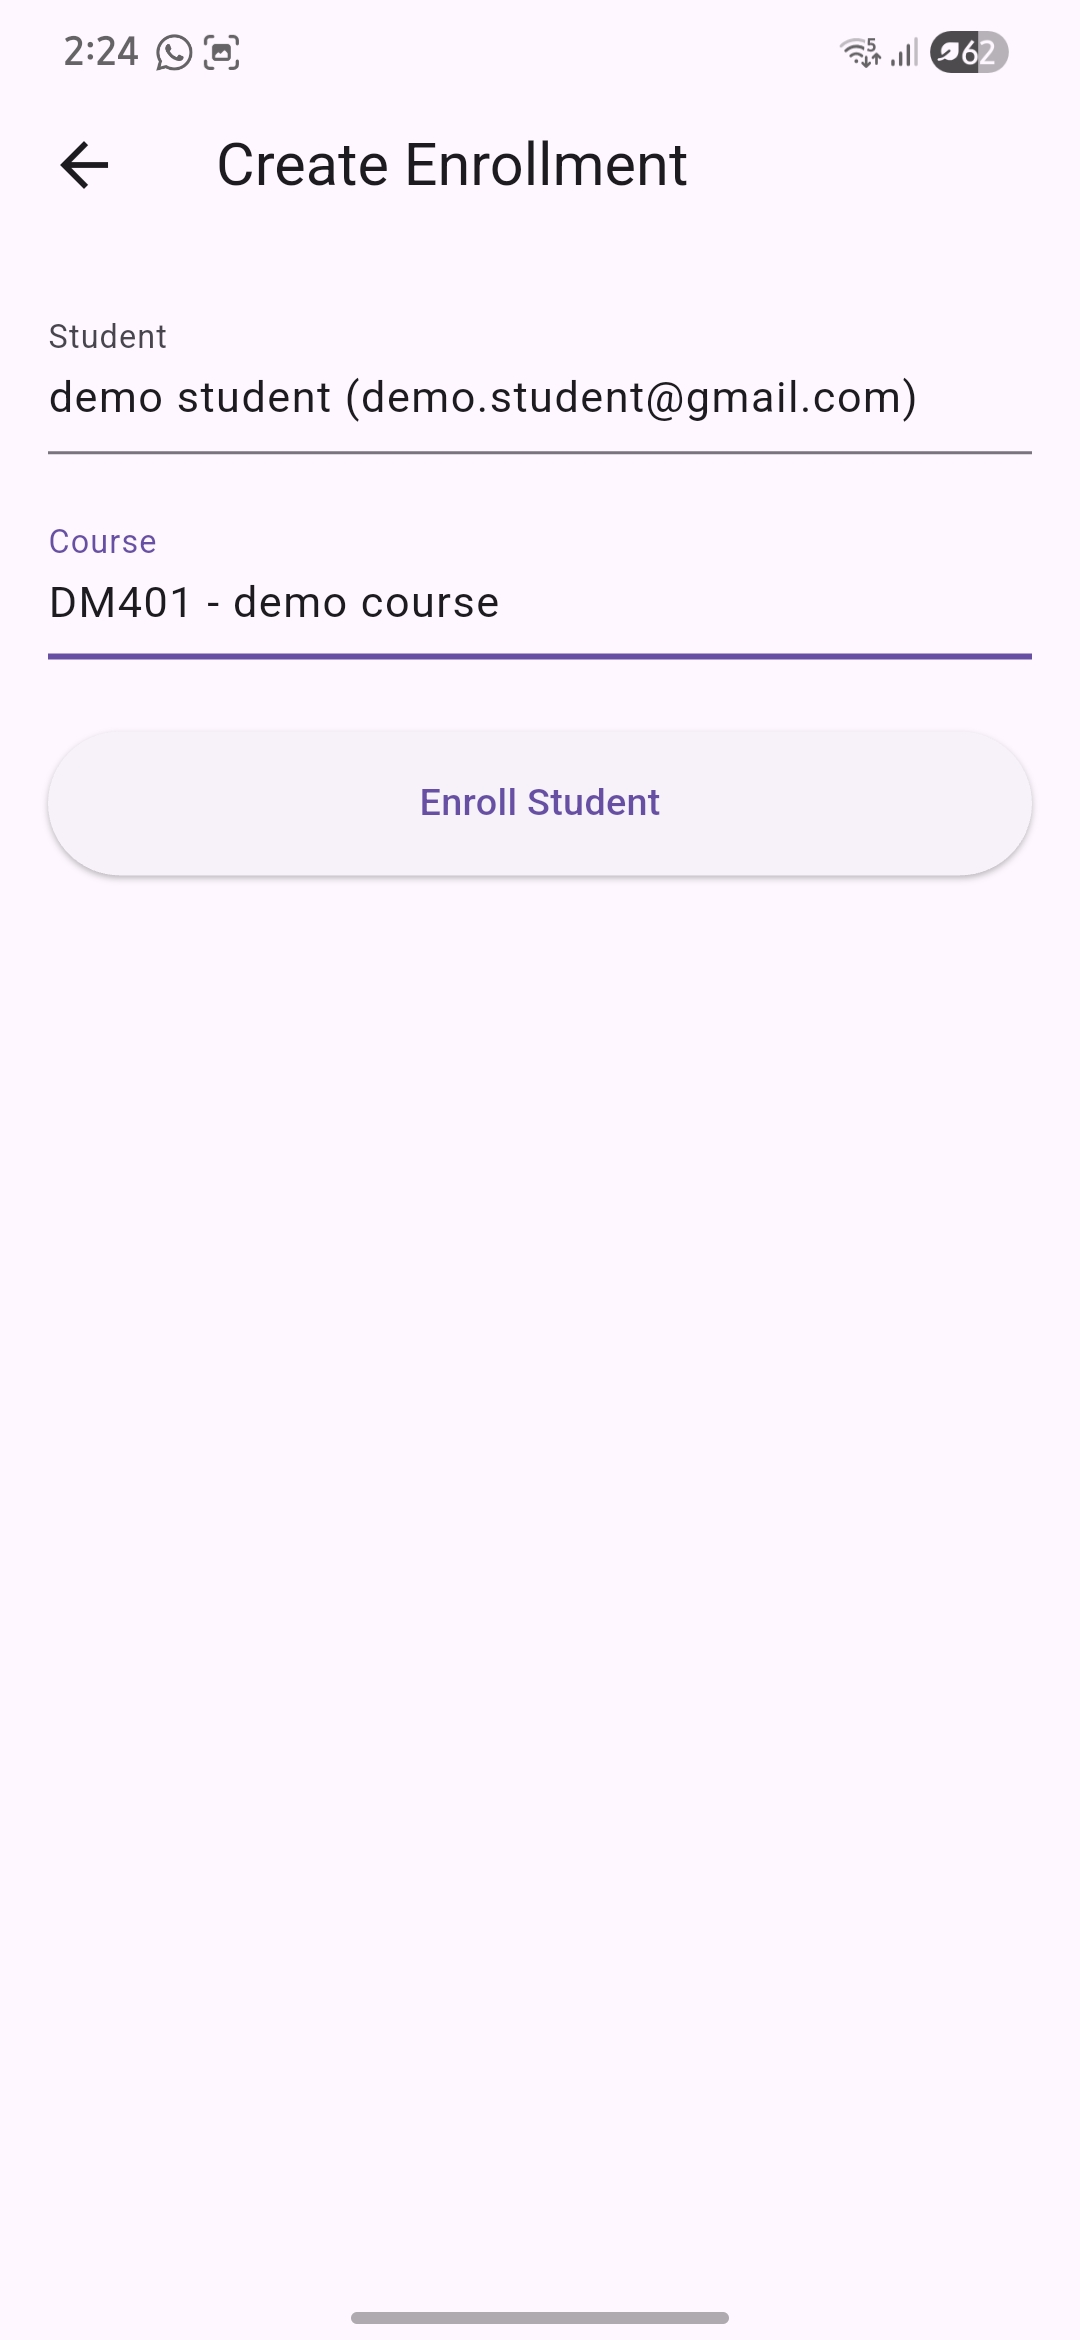
\includegraphics[width=0.48\textwidth]{images/screenshots/admin/ADM_05_enroll_student_01.jpeg}
    \hfill
    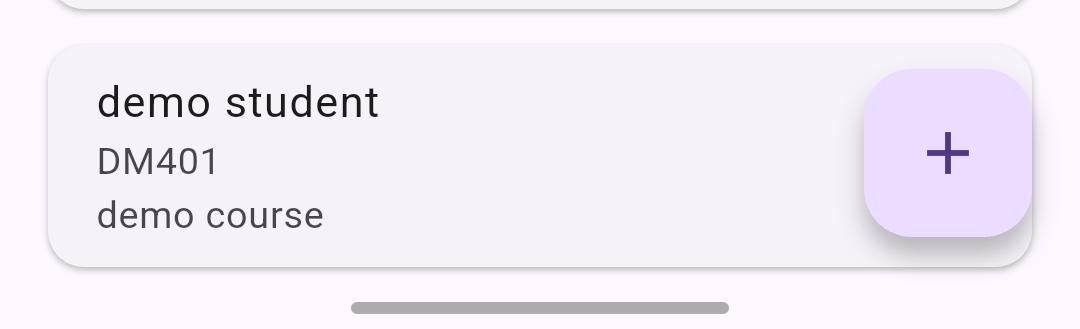
\includegraphics[width=0.48\textwidth]{images/screenshots/admin/ADM_05_enroll_student_02.jpeg}
    \caption{Admin: Enroll Student in Course (Step 1 and Step 2)}
    \label{fig:appD-adm-05}
\end{figure}

\begin{figure}[htbp]
    \centering
    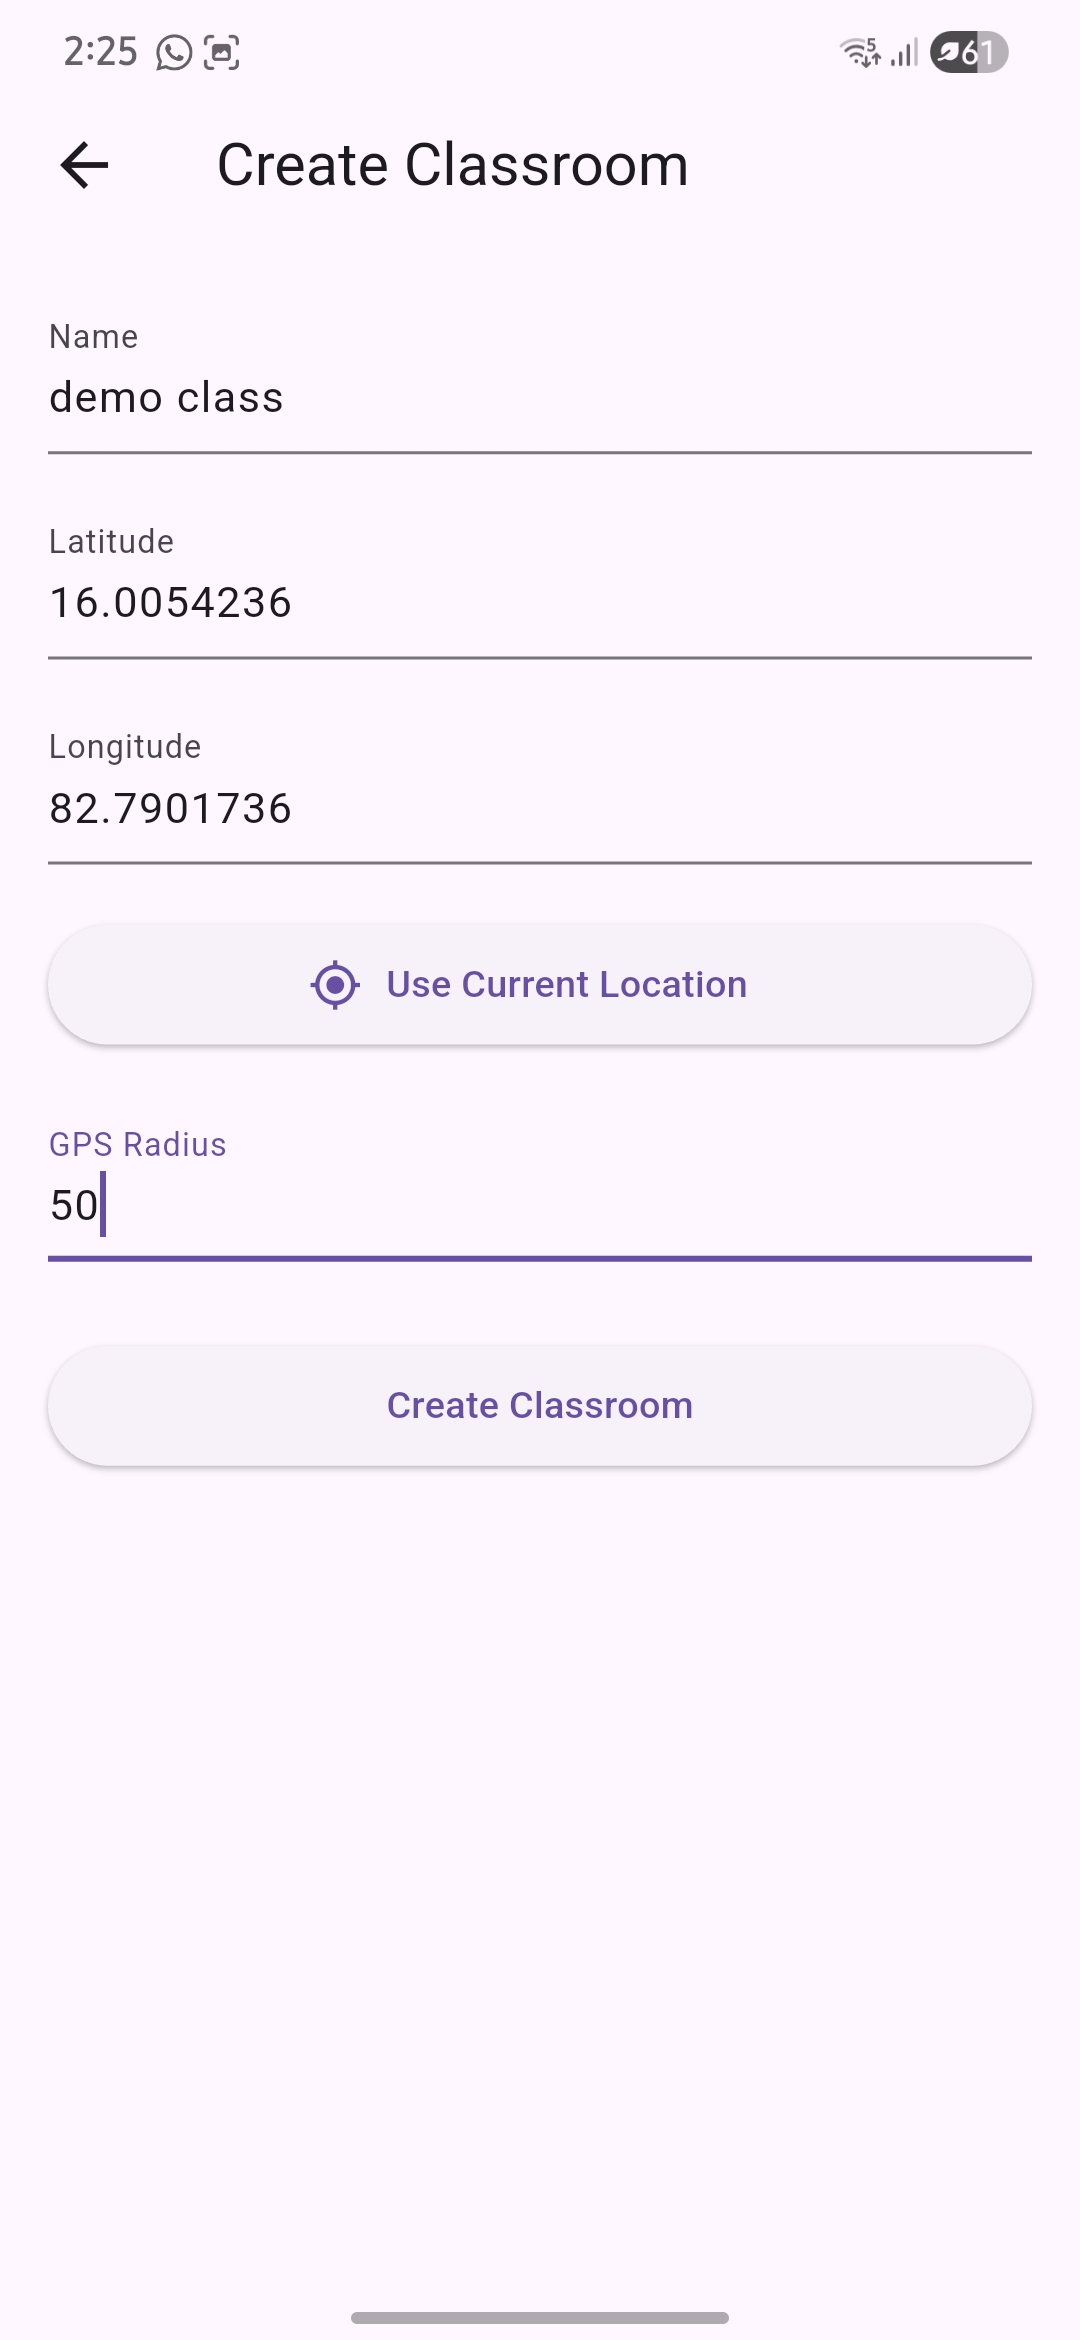
\includegraphics[width=0.48\textwidth]{images/screenshots/admin/ADM_06_create_classroom_01.jpeg}
    \hfill
    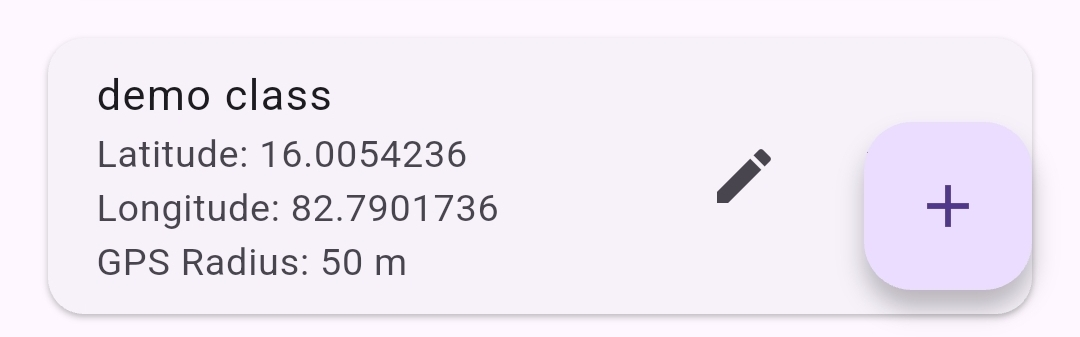
\includegraphics[width=0.48\textwidth]{images/screenshots/admin/ADM_06_create_classroom_02.jpeg}
    \caption{Admin: Create Classroom (Step 1 and Step 2)}
    \label{fig:appD-adm-06}
\end{figure}

\begin{figure}[htbp]
    \centering
    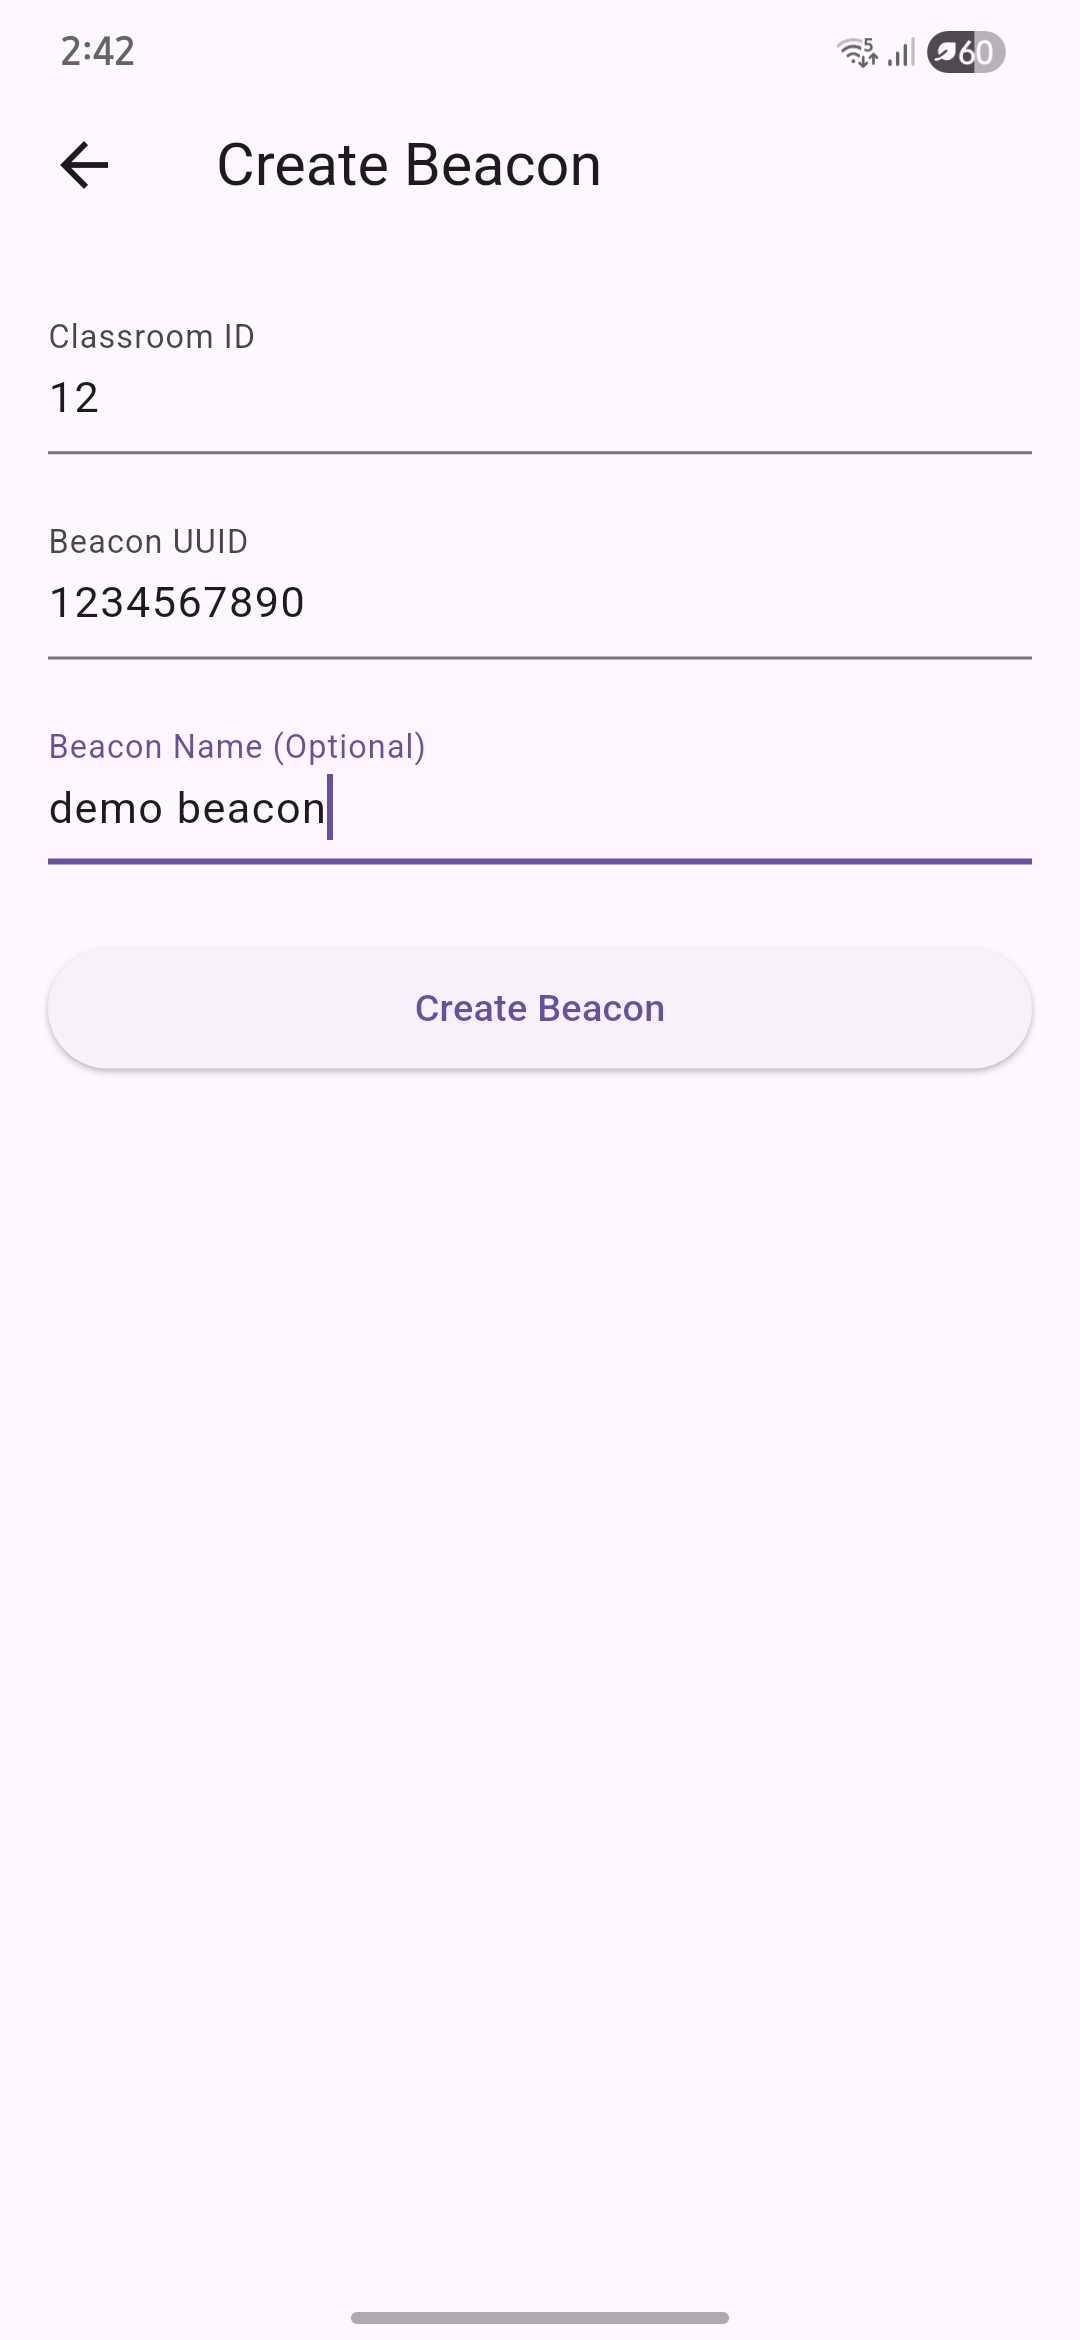
\includegraphics[width=0.48\textwidth]{images/screenshots/admin/ADM_07_assign_beacon_01.jpeg}
    \hfill
    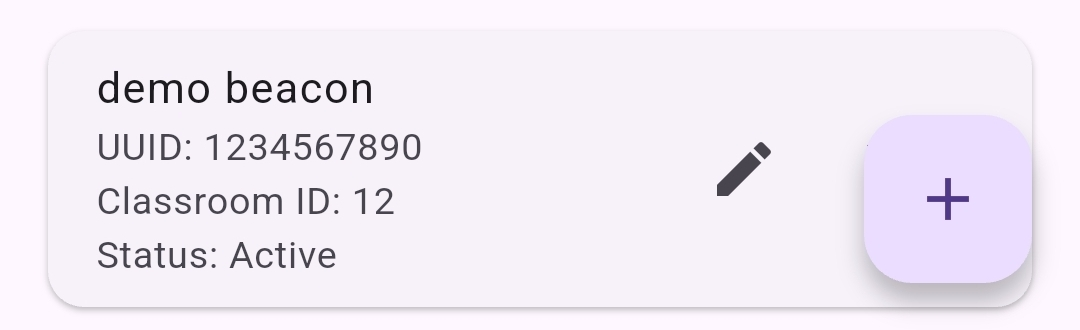
\includegraphics[width=0.48\textwidth]{images/screenshots/admin/ADM_07_assign_beacon_02.jpeg}
    \caption{Admin: Assign BLE Beacon to Classroom (Step 1 and Step 2)}
    \label{fig:appD-adm-07}
\end{figure}

\begin{figure}[htbp]
    \centering
    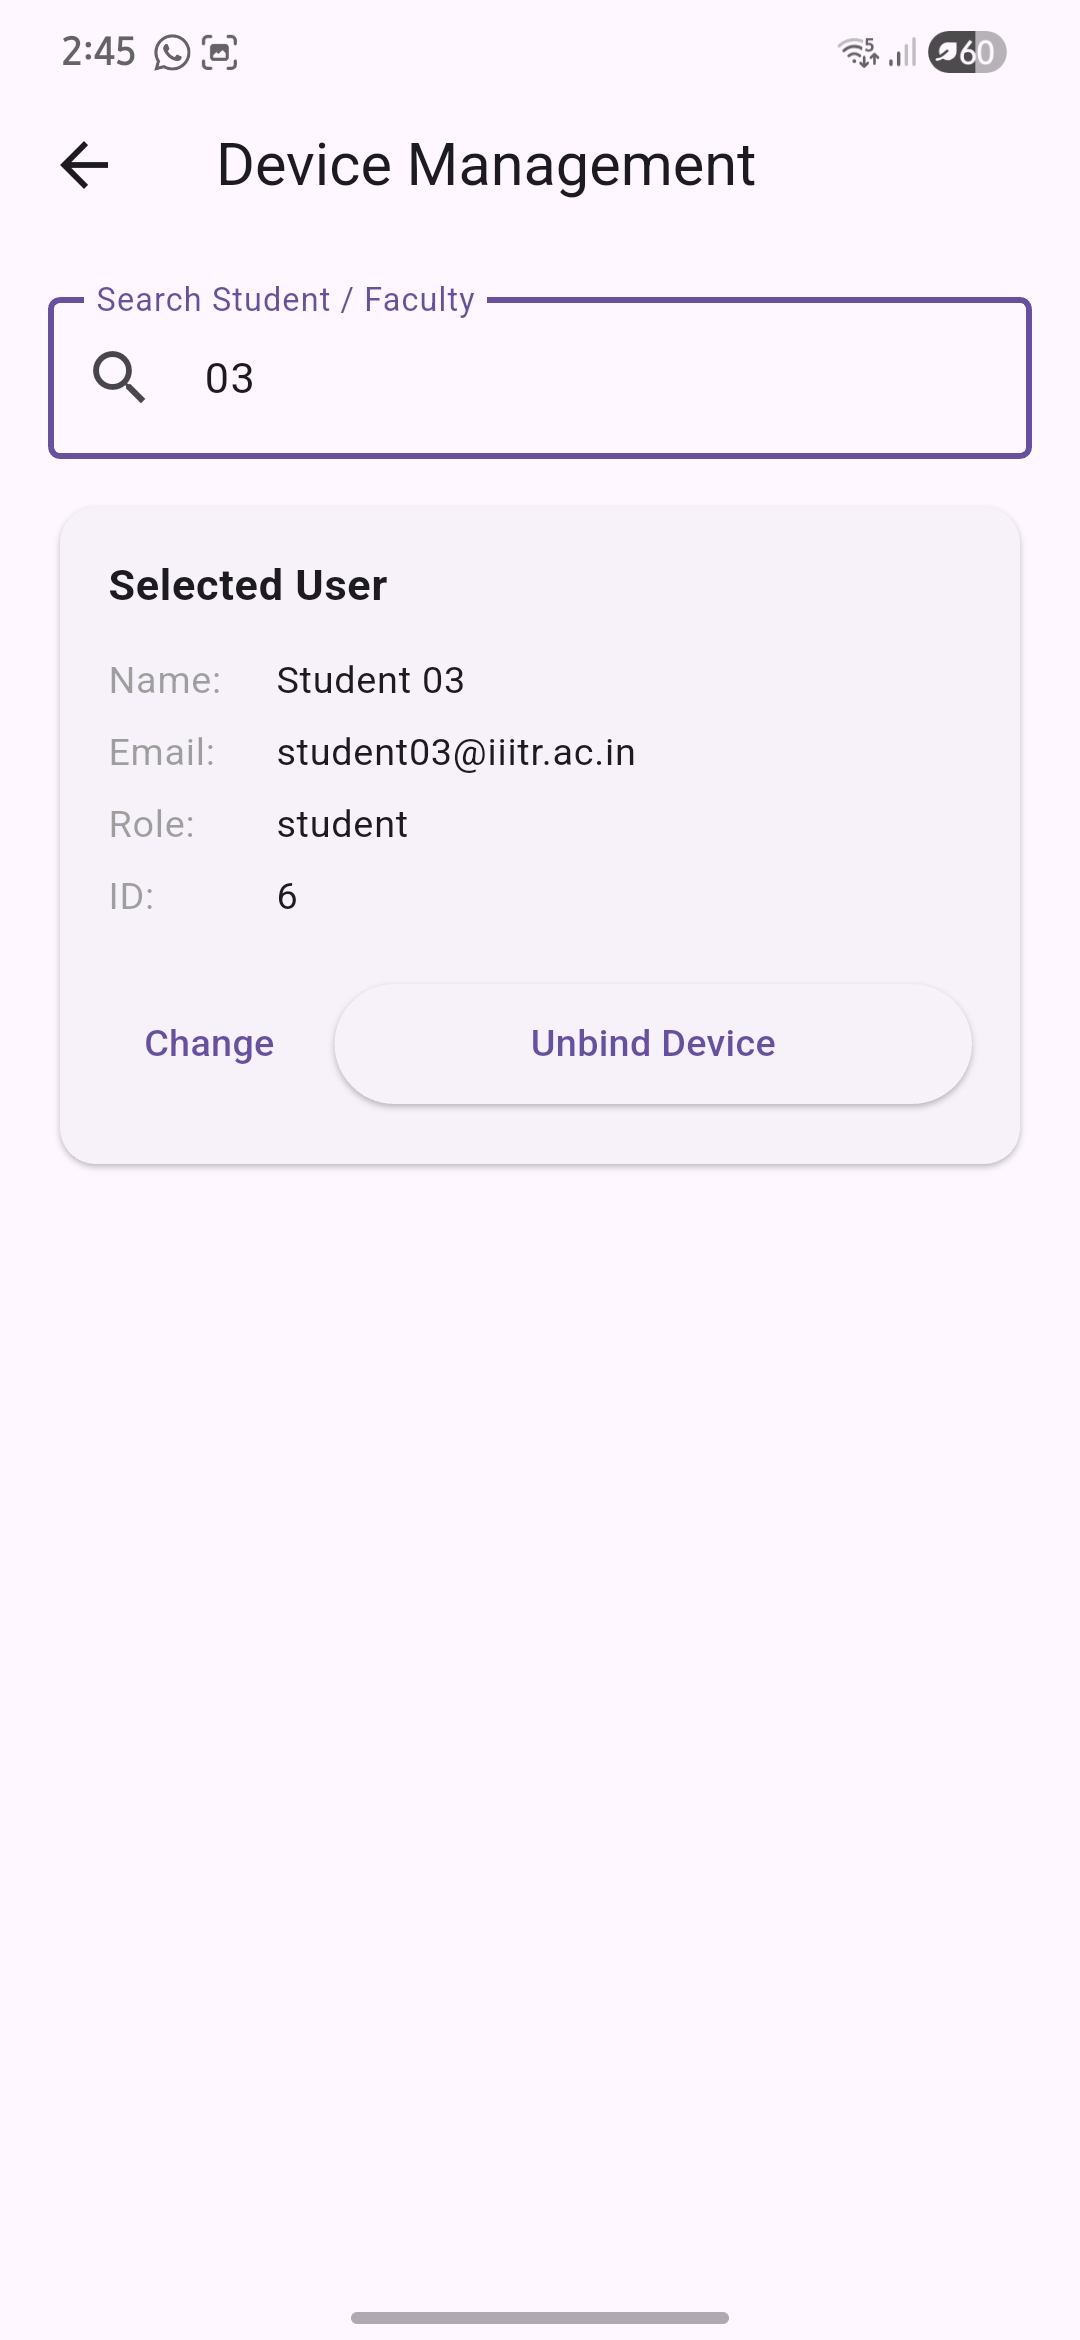
\includegraphics[width=0.48\textwidth]{images/screenshots/admin/ADM_08_unbind_device_01.jpeg}
    \hfill
    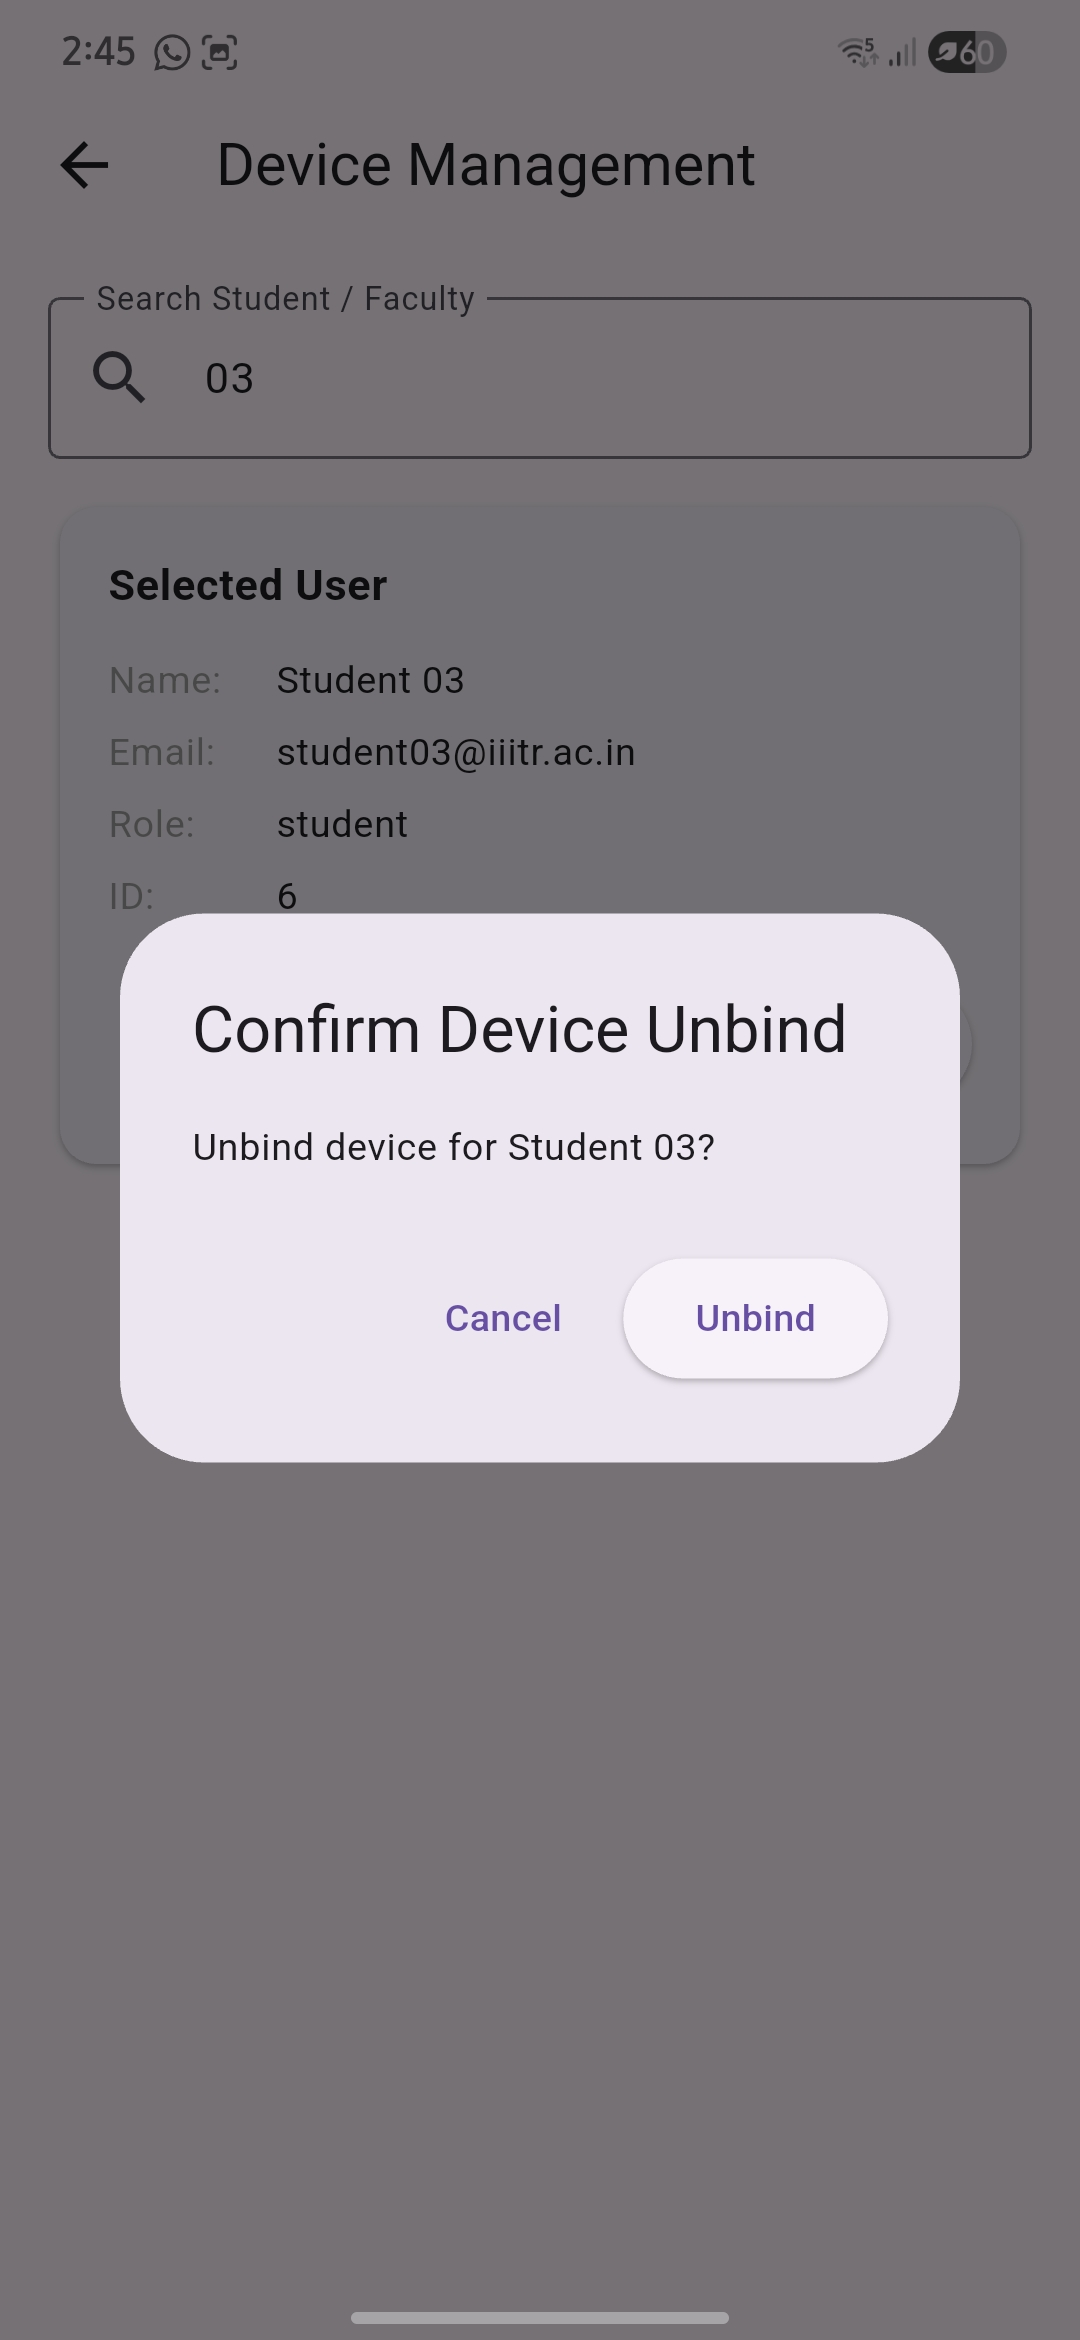
\includegraphics[width=0.48\textwidth]{images/screenshots/admin/ADM_08_unbind_device_02.jpeg}
    \caption{Admin: Unbind Student Device (Step 1 and Step 2)}
    \label{fig:appD-adm-08}
\end{figure}

\begin{figure}[htbp]
    \centering
    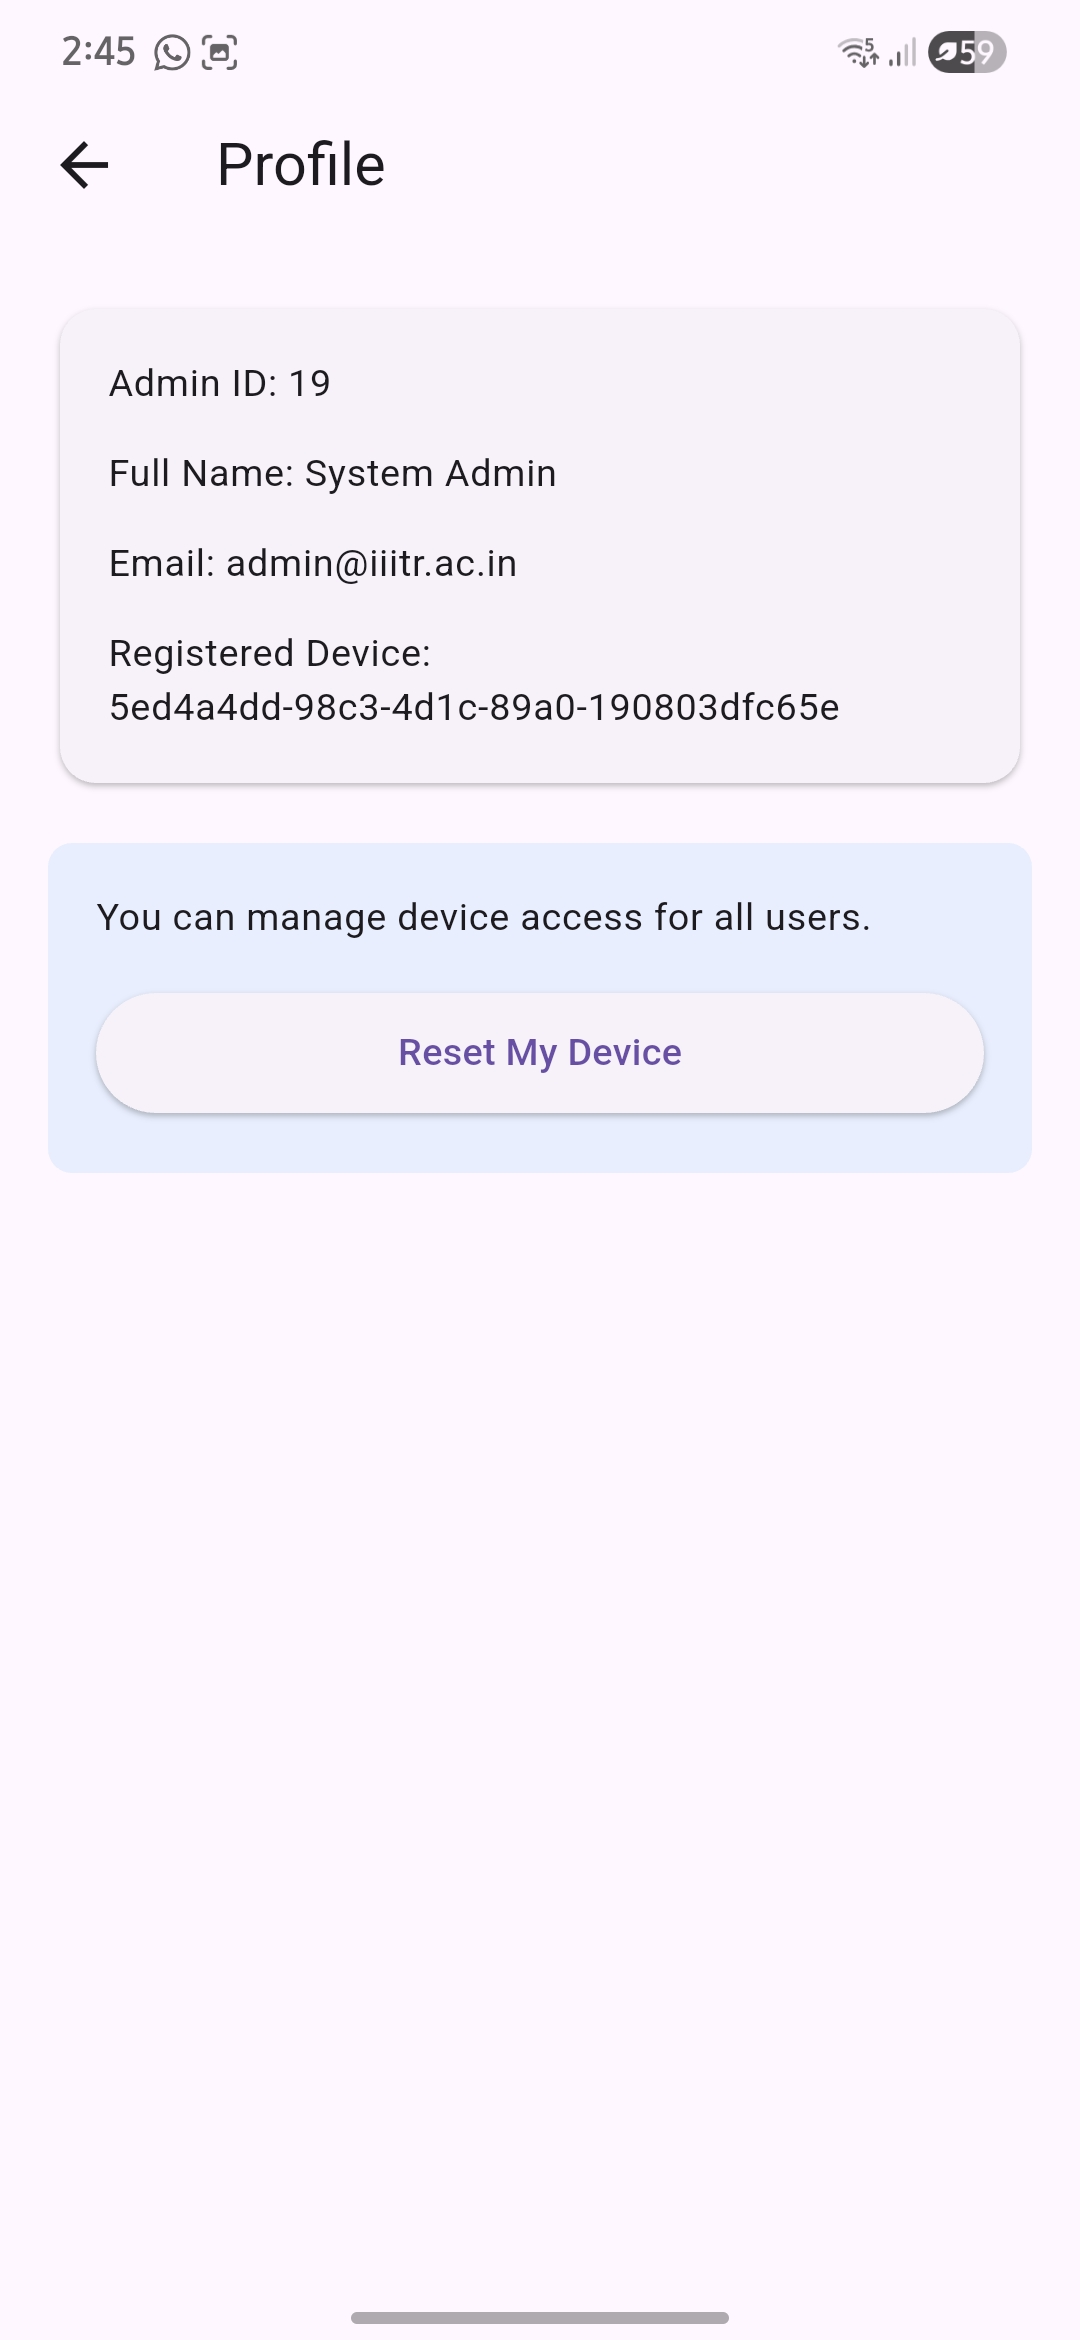
\includegraphics[width=0.48\textwidth]{images/screenshots/admin/ADM_09_self_unbind_device_01.jpeg}
    \hfill
    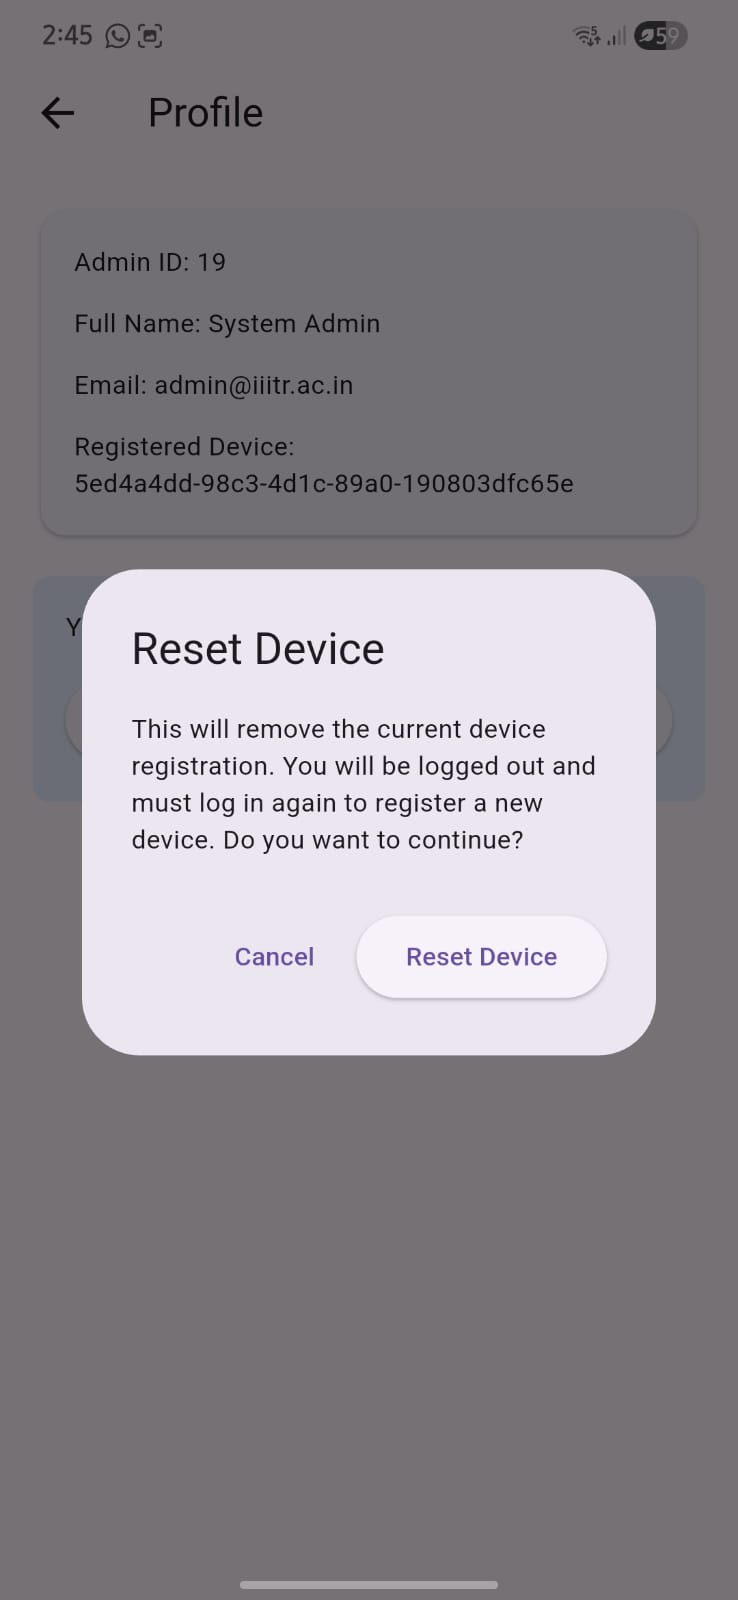
\includegraphics[width=0.48\textwidth]{images/screenshots/admin/ADM_09_self_unbind_device_02.jpeg}
    \caption{Admin: Self-Service Device Unbind (Step 1 and Step 2)}
    \label{fig:appD-adm-09}
\end{figure}

\section{Faculty Screenshots}
\label{app:screenshots-faculty}

\begin{figure}[htbp]
    \centering
    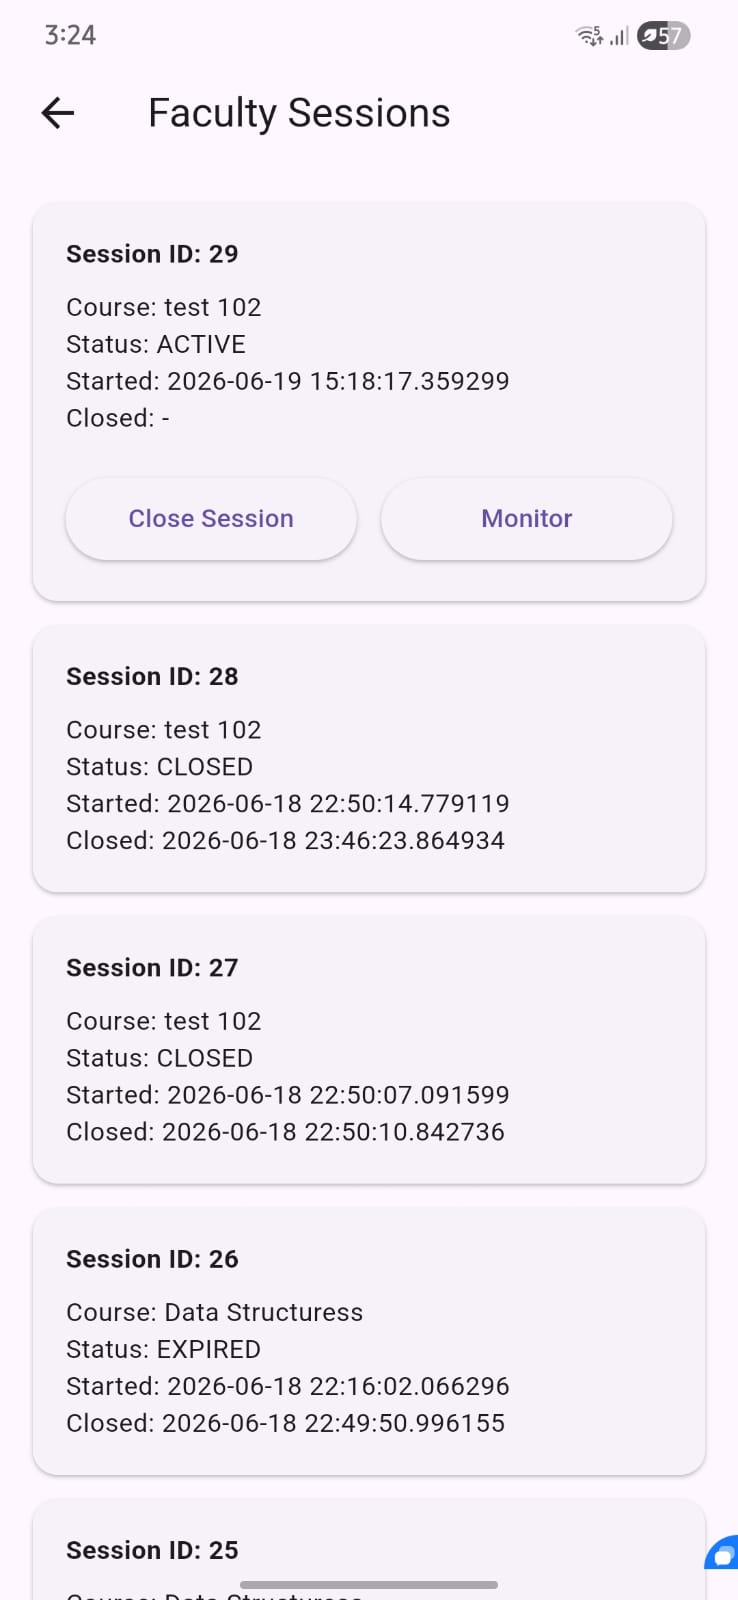
\includegraphics[width=0.7\textwidth]{images/screenshots/faculty/FAC_01_faculty_sessions.jpeg}
    \caption{Faculty: Session Dashboard}
    \label{fig:appD-fac-01}
\end{figure}

\begin{figure}[htbp]
    \centering
    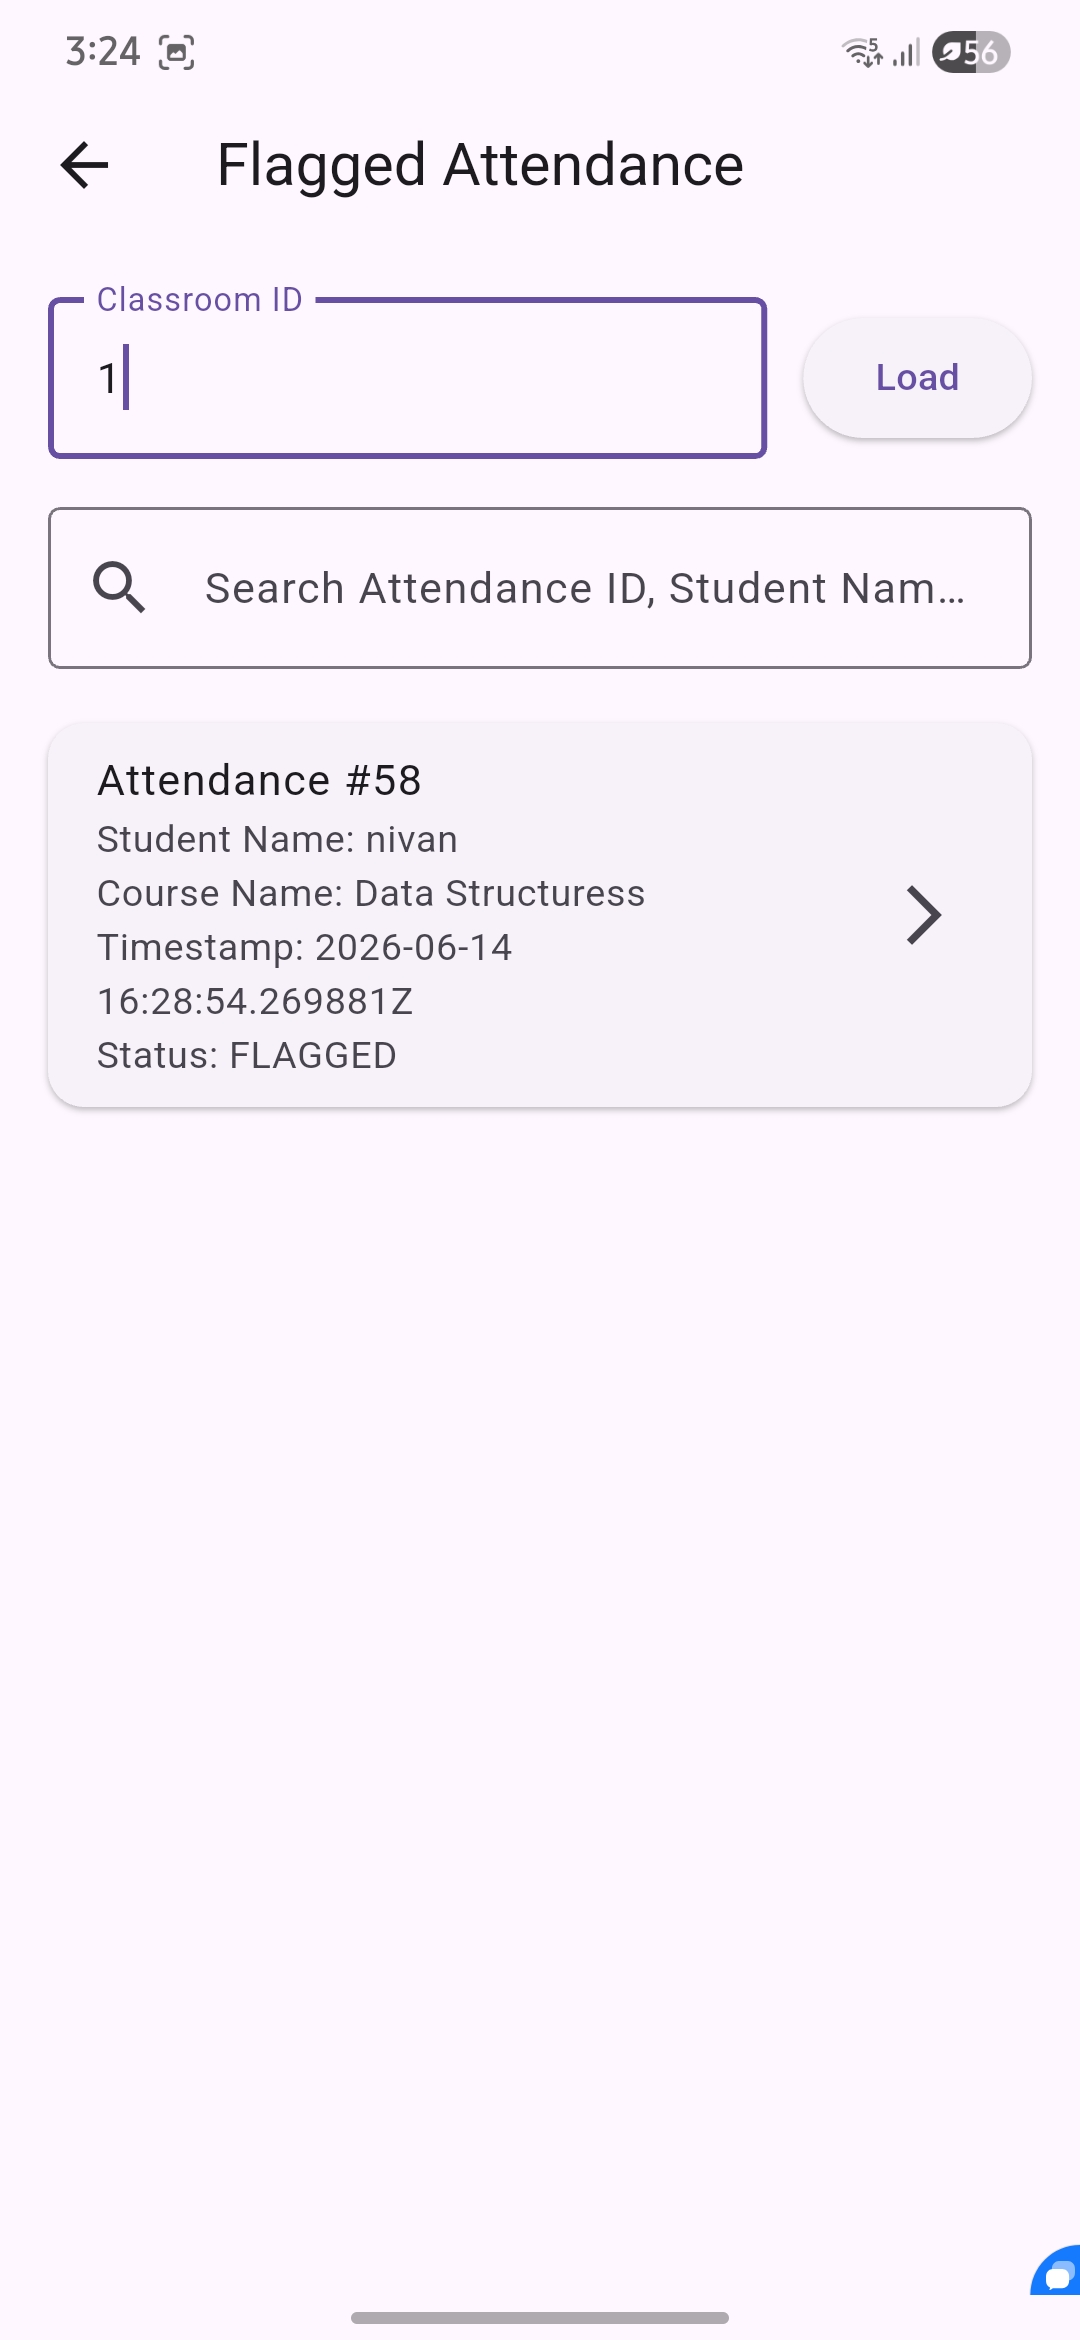
\includegraphics[width=0.7\textwidth]{images/screenshots/faculty/FAC_02_flagged_attendance_list.jpeg}
    \caption{Faculty: Flagged Attendance List}
    \label{fig:appD-fac-02}
\end{figure}

\begin{figure}[htbp]
    \centering
    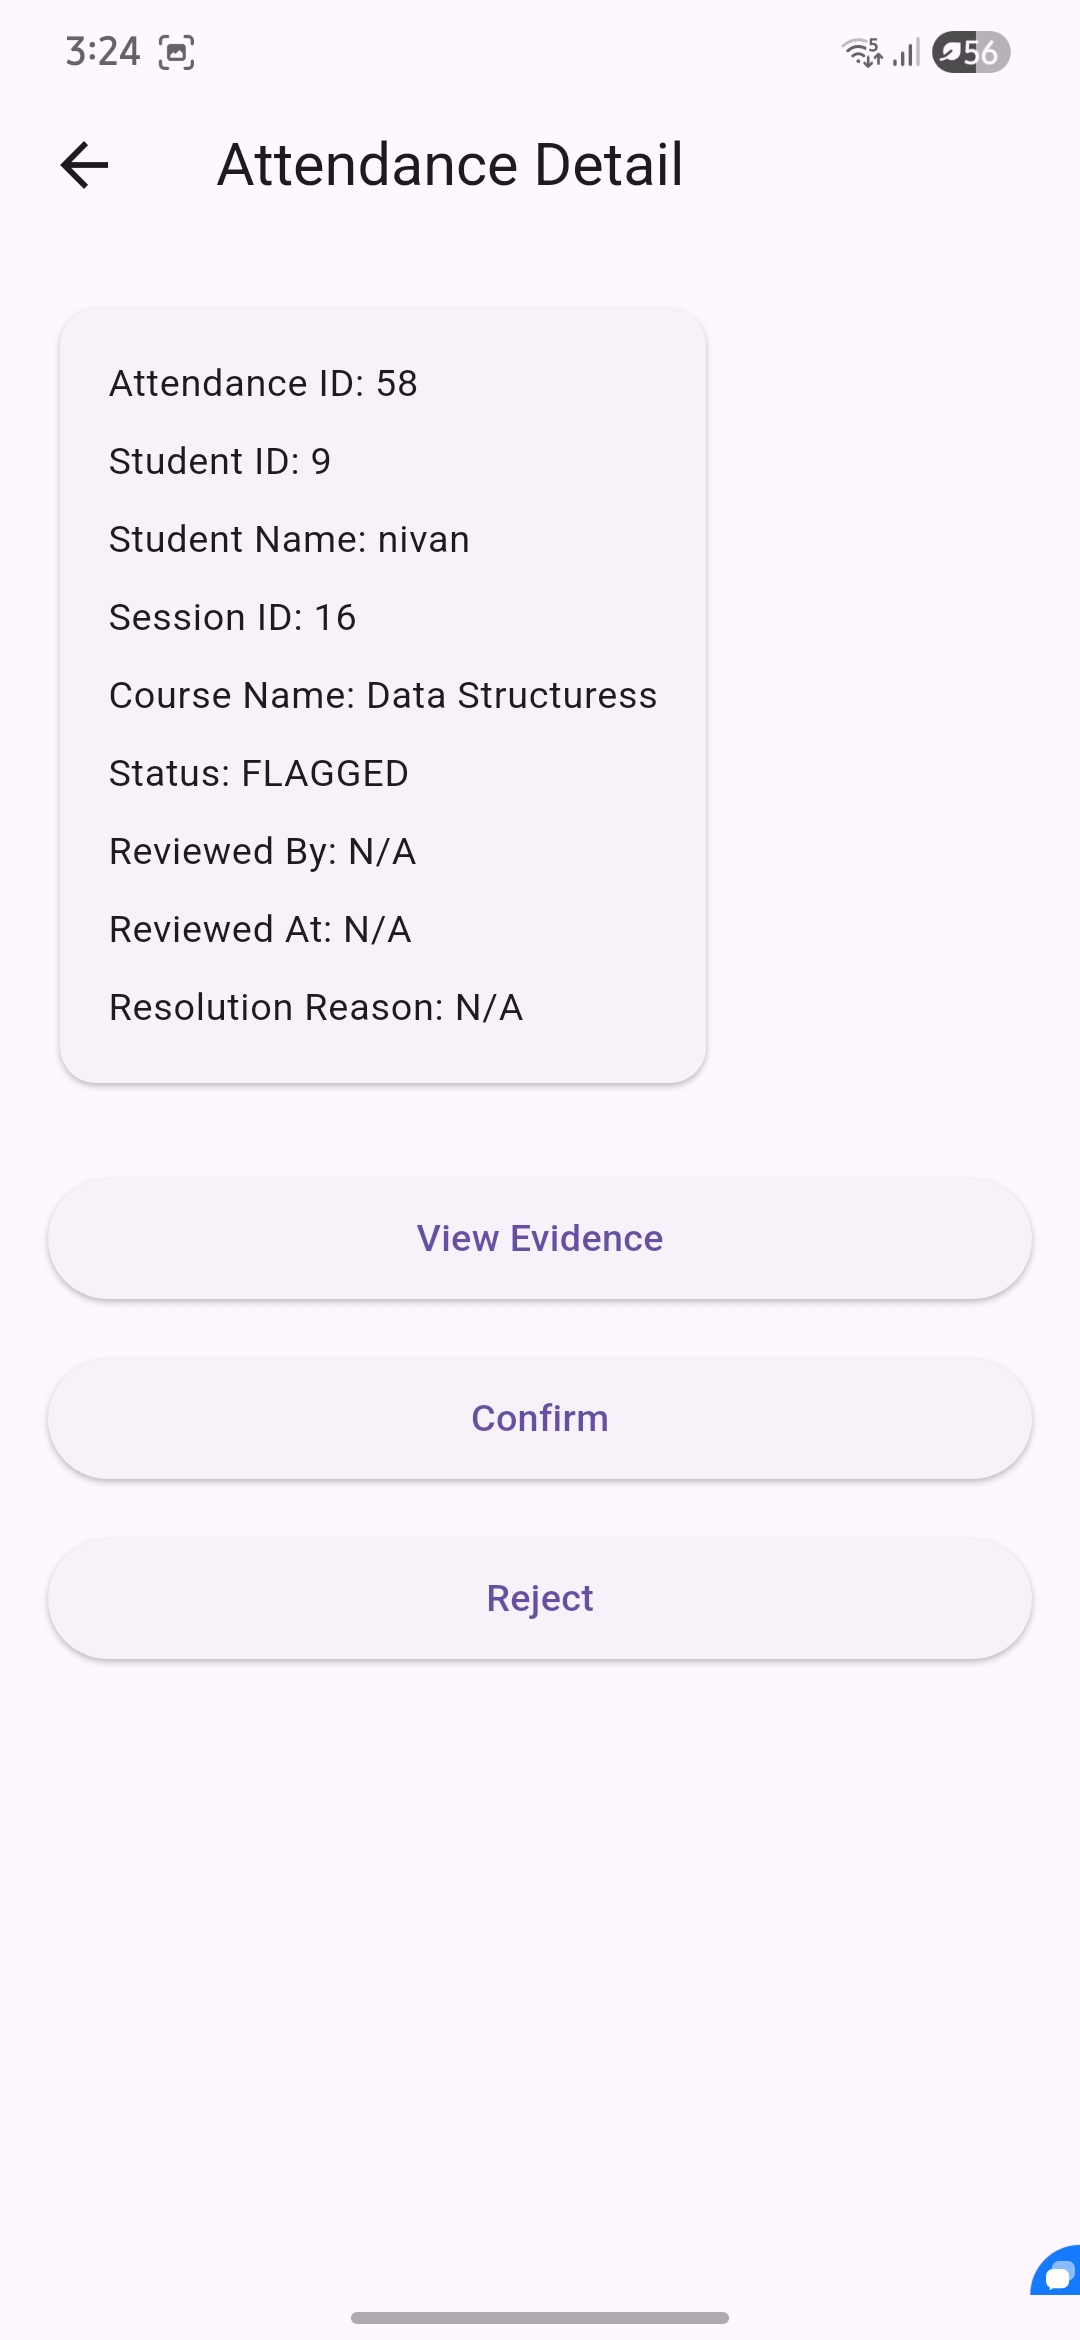
\includegraphics[width=0.7\textwidth]{images/screenshots/faculty/FAC_03_attendance_detail_flagged.jpeg}
    \caption{Faculty: Flagged Attendance Detail (BLE/GPS Evidence Review)}
    \label{fig:appD-fac-03}
\end{figure}

\begin{figure}[htbp]
    \centering
    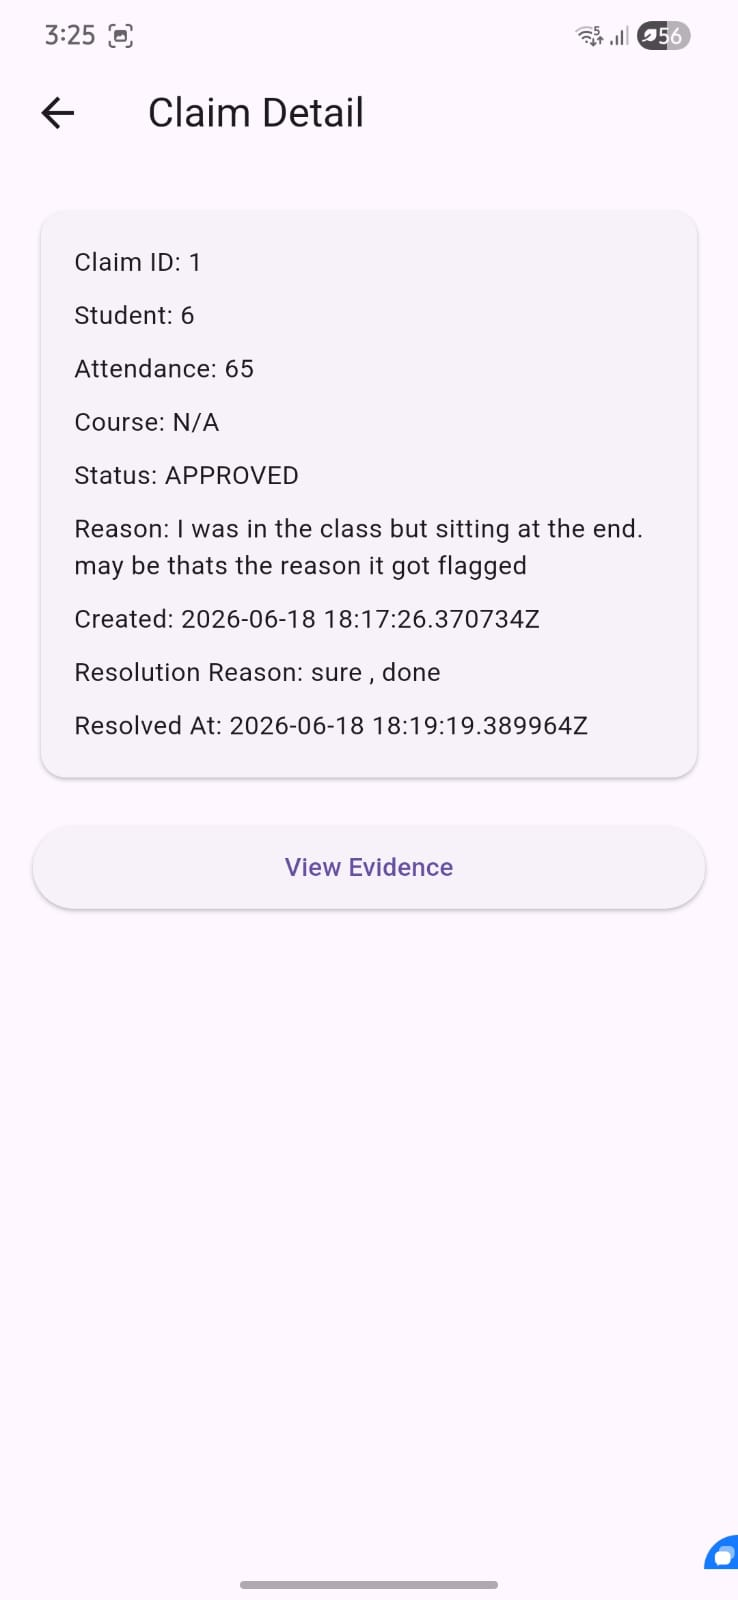
\includegraphics[width=0.7\textwidth]{images/screenshots/faculty/FAC_04_attendance_confirmed.jpeg}
    \caption{Faculty: Attendance Confirmed After Review}
    \label{fig:appD-fac-04}
\end{figure}

\begin{figure}[htbp]
    \centering
    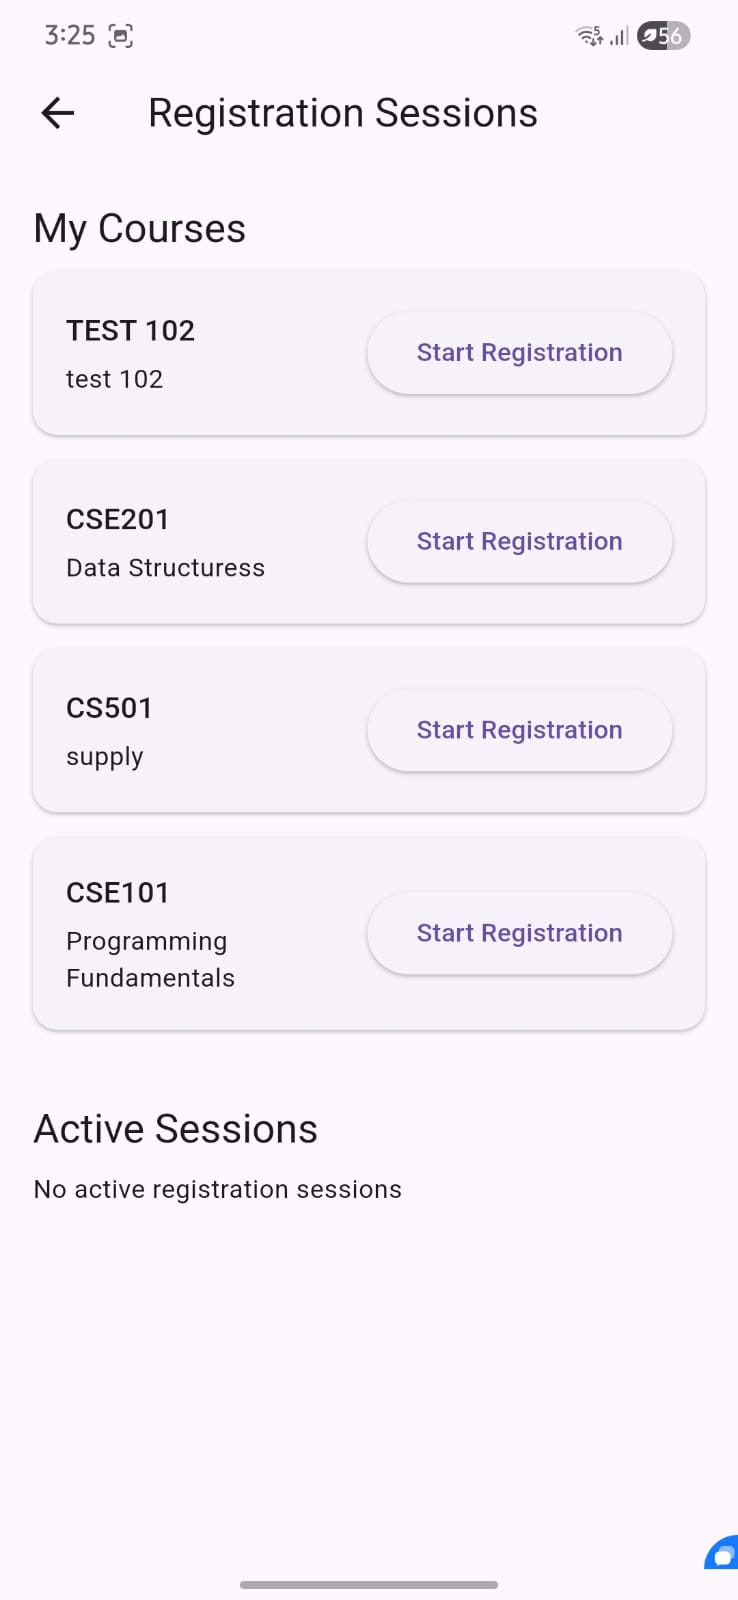
\includegraphics[width=0.7\textwidth]{images/screenshots/faculty/FAC_05_registration_sessions.jpeg}
    \caption{Faculty: Registration Sessions}
    \label{fig:appD-fac-05}
\end{figure}

\begin{figure}[htbp]
    \centering
    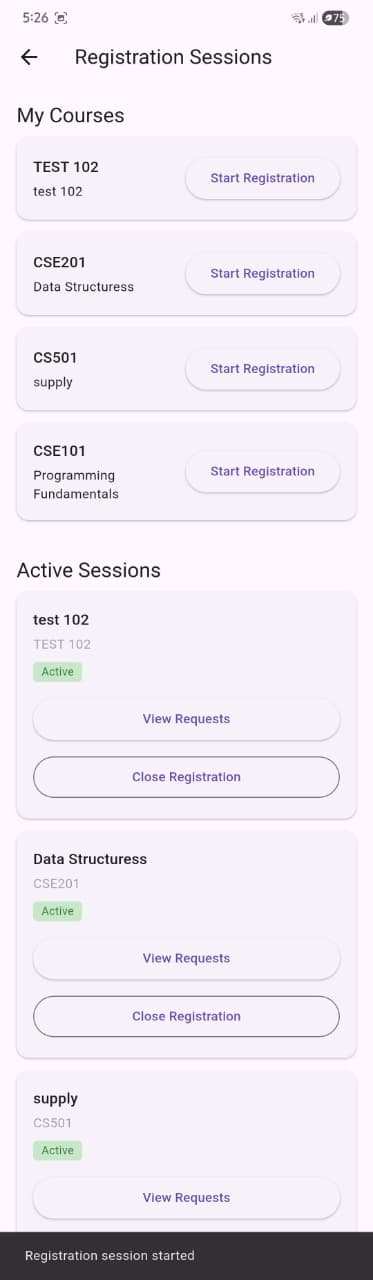
\includegraphics[width=0.7\textwidth]{images/screenshots/faculty/FAC_06_registration_session_management.jpeg}
    \caption{Faculty: Registration Session Management}
    \label{fig:appD-fac-06}
\end{figure}

\begin{figure}[htbp]
    \centering
    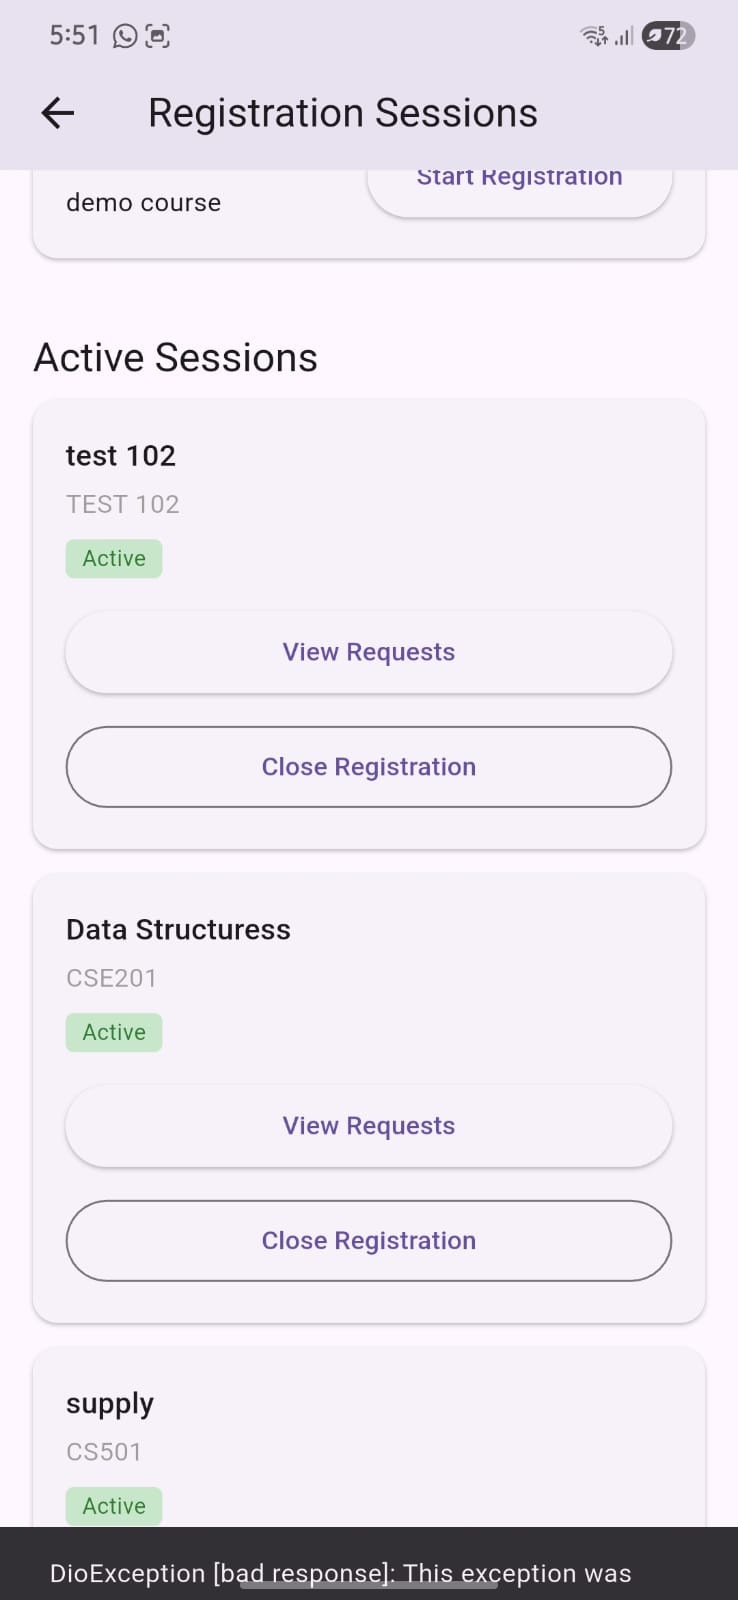
\includegraphics[width=0.7\textwidth]{images/screenshots/faculty/FAC_07_registration_sessions_error.jpeg}
    \caption{Faculty: Registration Session Error Handling}
    \label{fig:appD-fac-07}
\end{figure}

\begin{figure}[htbp]
    \centering
    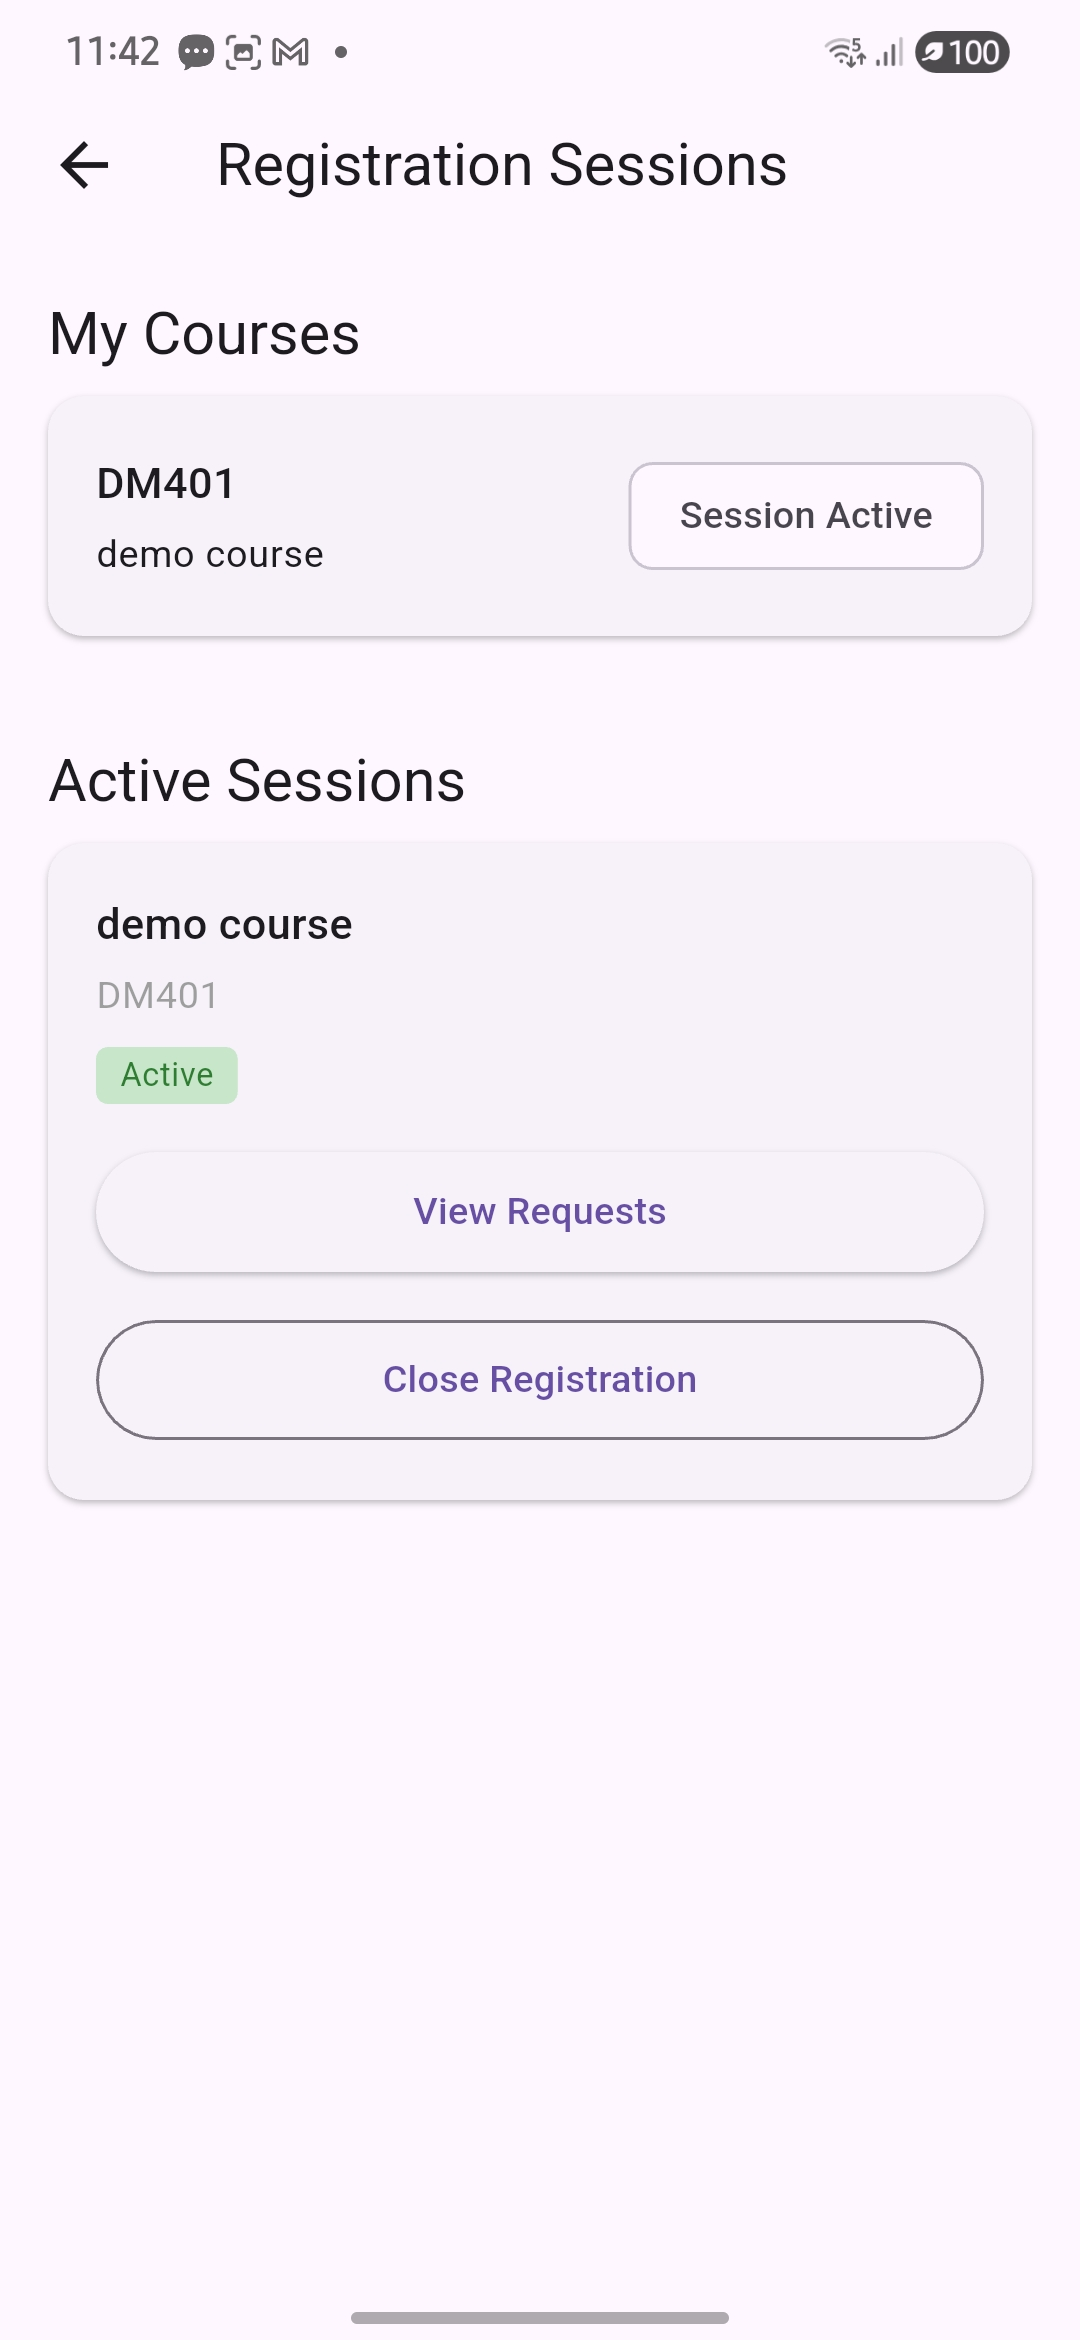
\includegraphics[width=0.7\textwidth]{images/screenshots/faculty/FAC_08_registration_session_active.jpeg}
    \caption{Faculty: Active Registration Session}
    \label{fig:appD-fac-08}
\end{figure}

\begin{figure}[htbp]
    \centering
    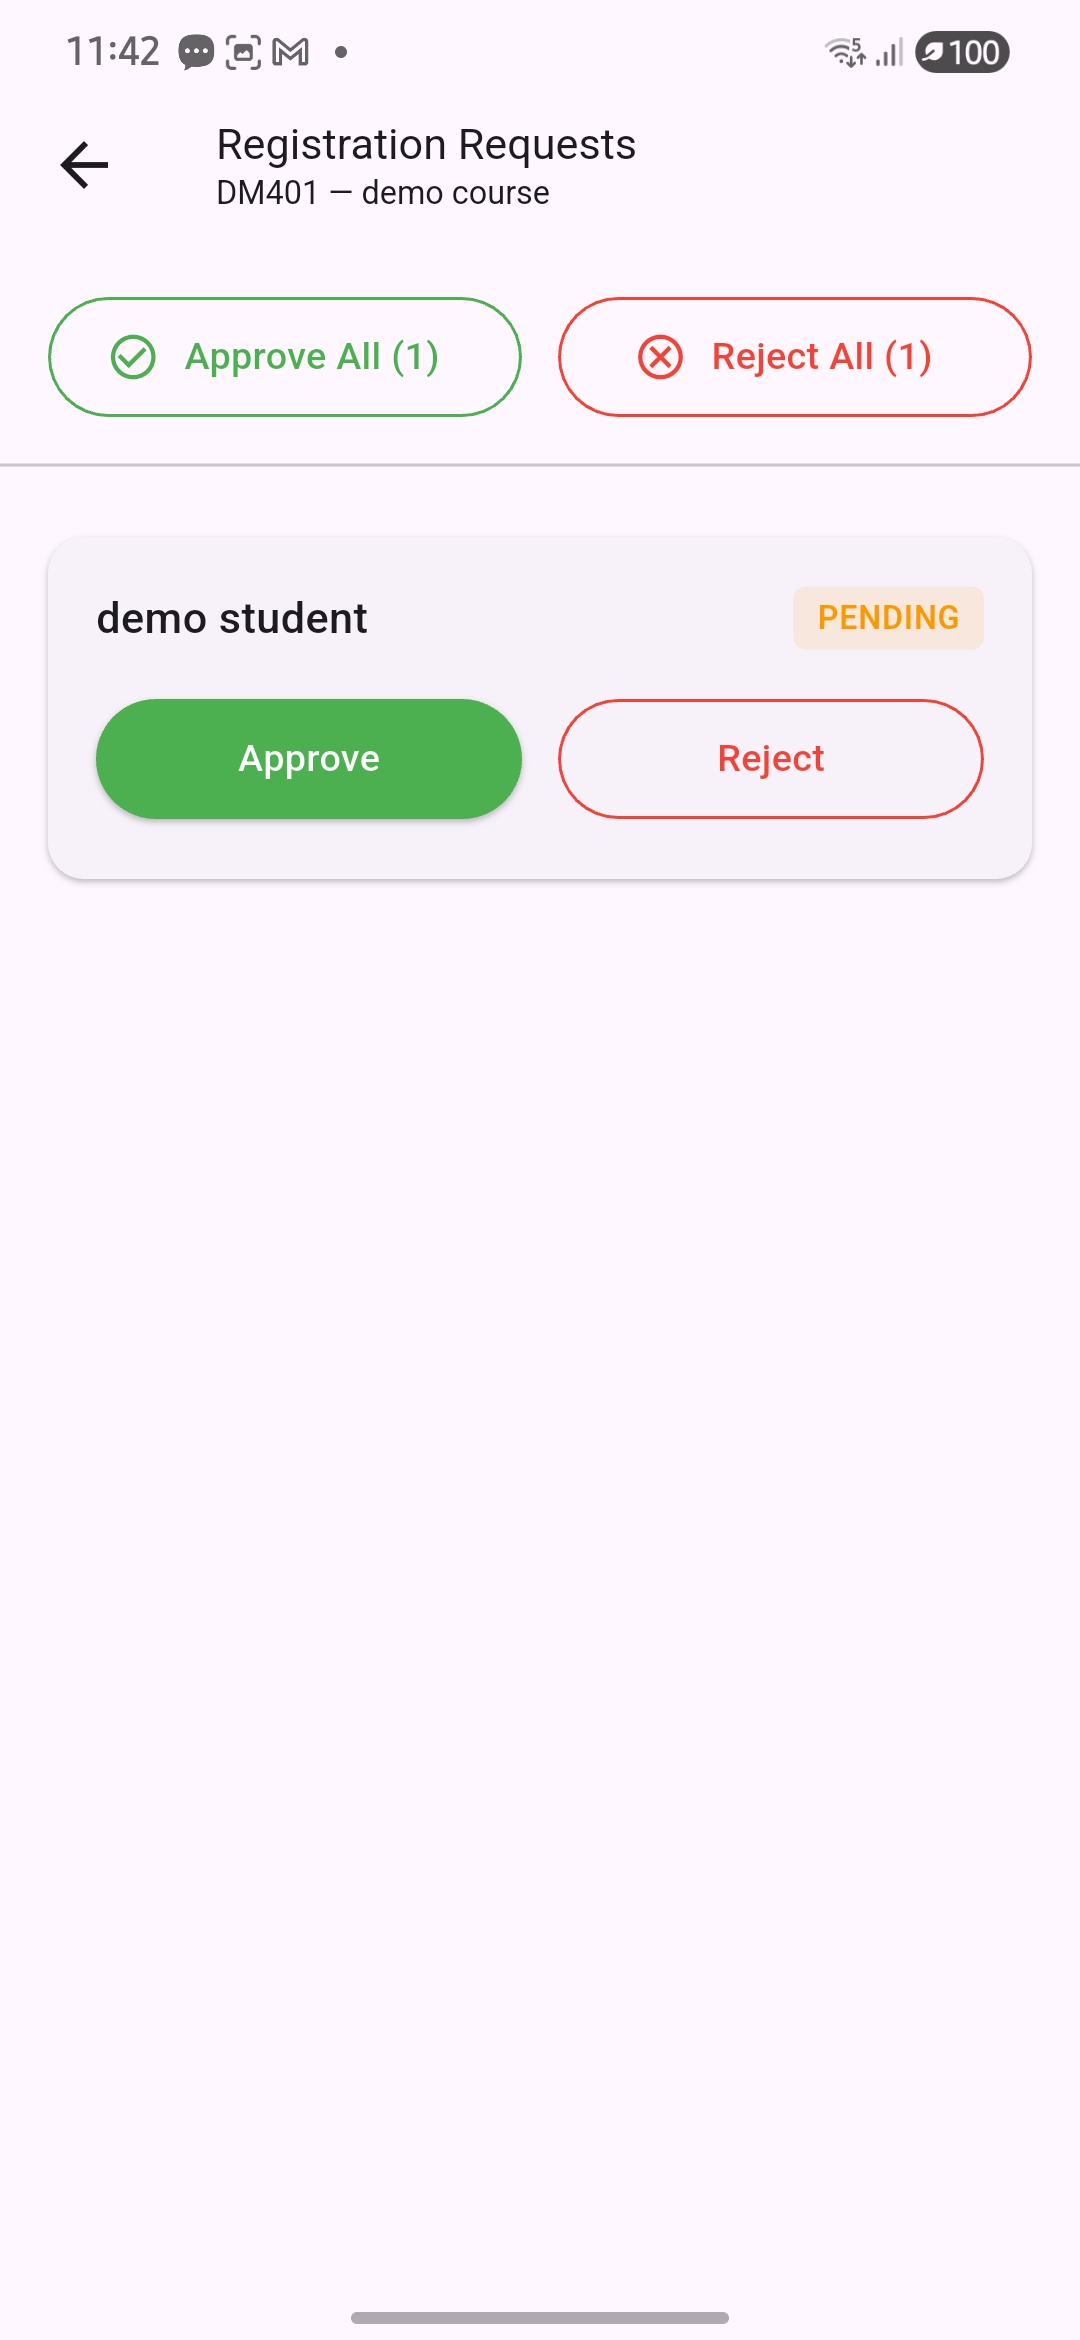
\includegraphics[width=0.7\textwidth]{images/screenshots/faculty/FAC_09_registration_request_pending.jpeg}
    \caption{Faculty: Pending Course Registration Request}
    \label{fig:appD-fac-09}
\end{figure}

\begin{figure}[htbp]
    \centering
    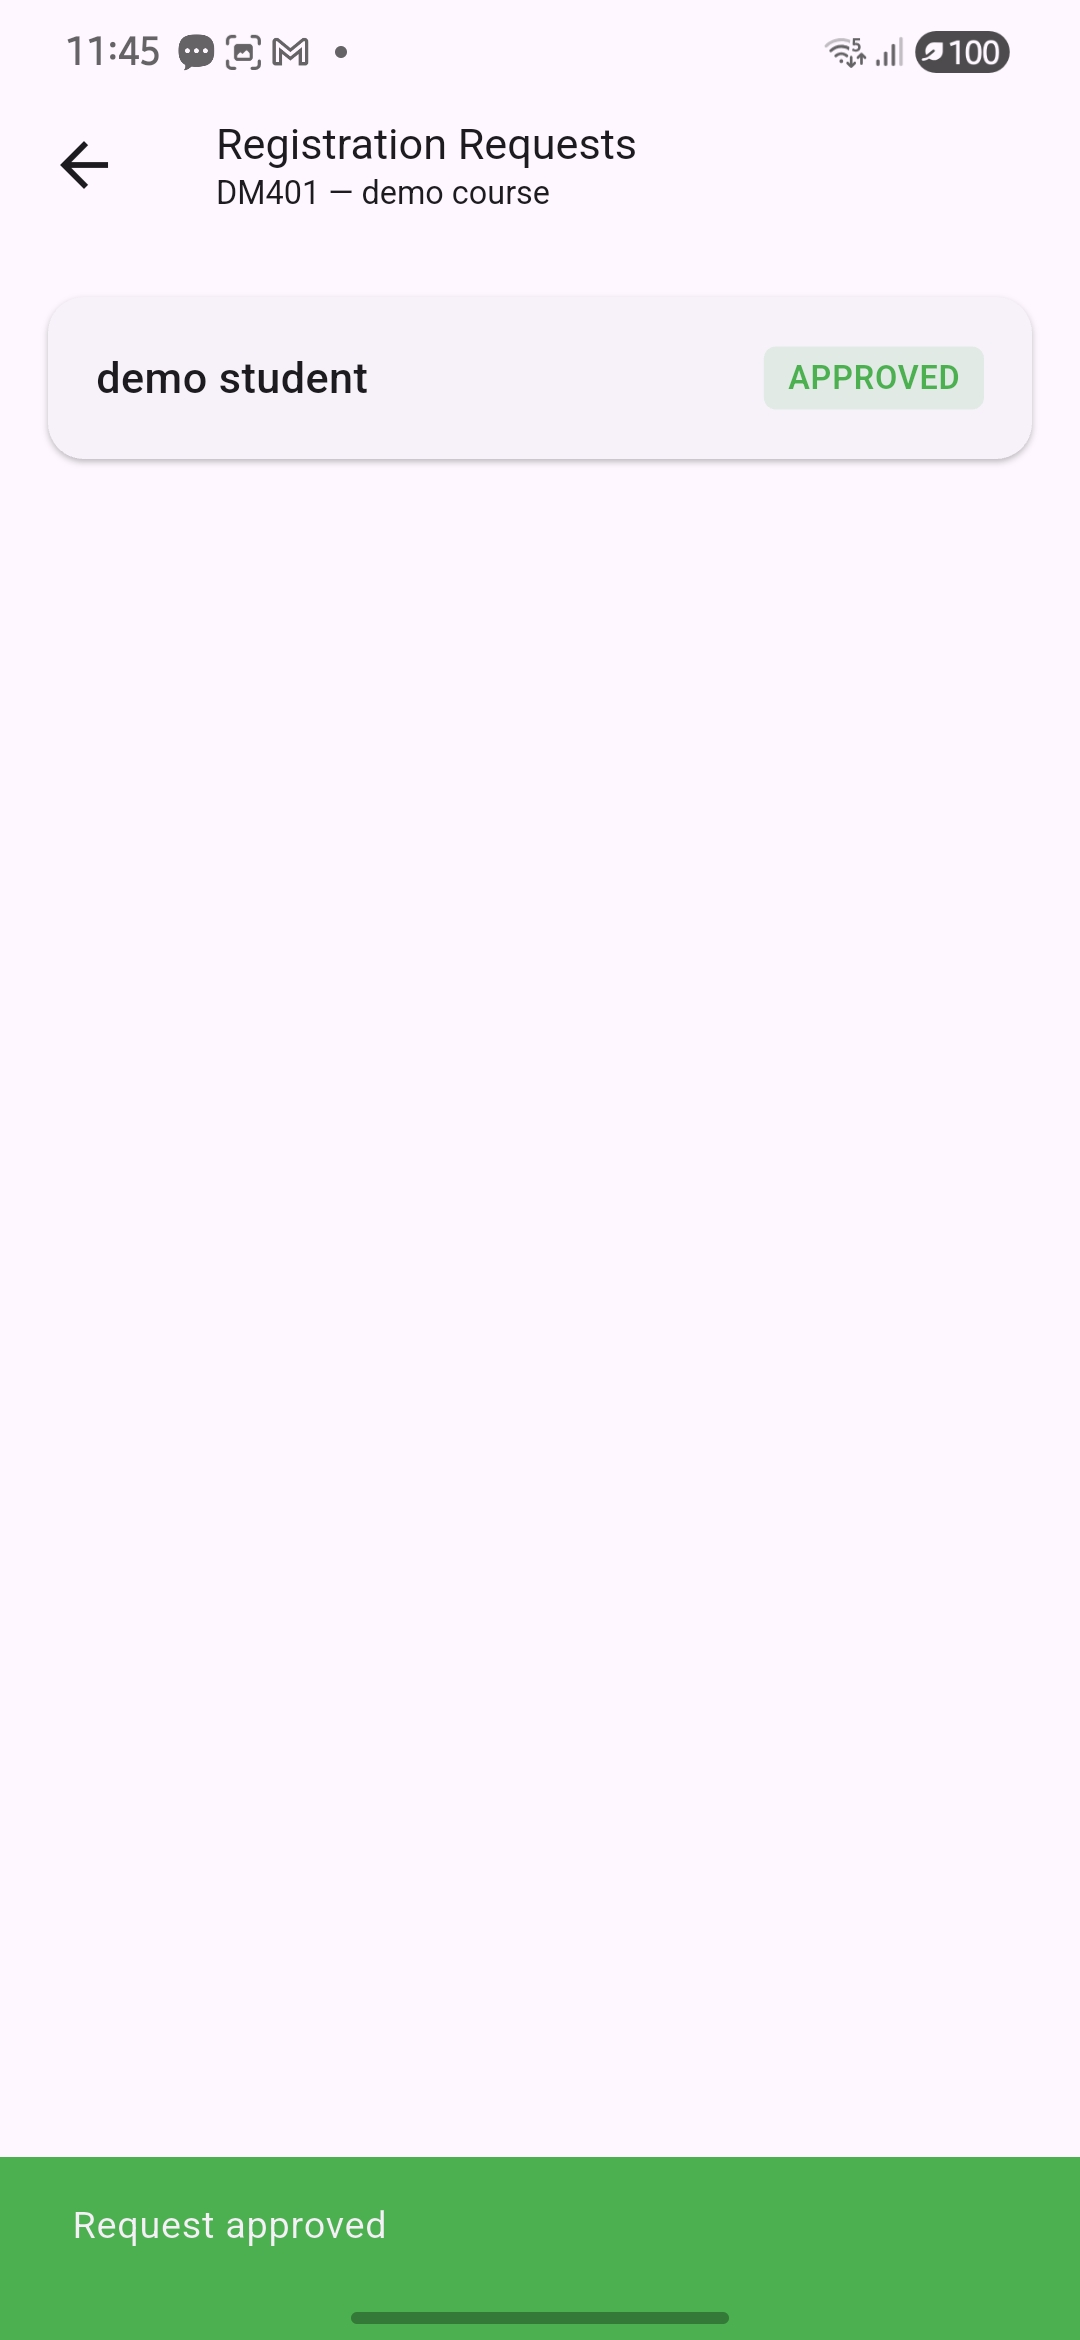
\includegraphics[width=0.7\textwidth]{images/screenshots/faculty/FAC_10_registration_request_approved.jpeg}
    \caption{Faculty: Approved Course Registration Request}
    \label{fig:appD-fac-10}
\end{figure}

\begin{figure}[htbp]
    \centering
    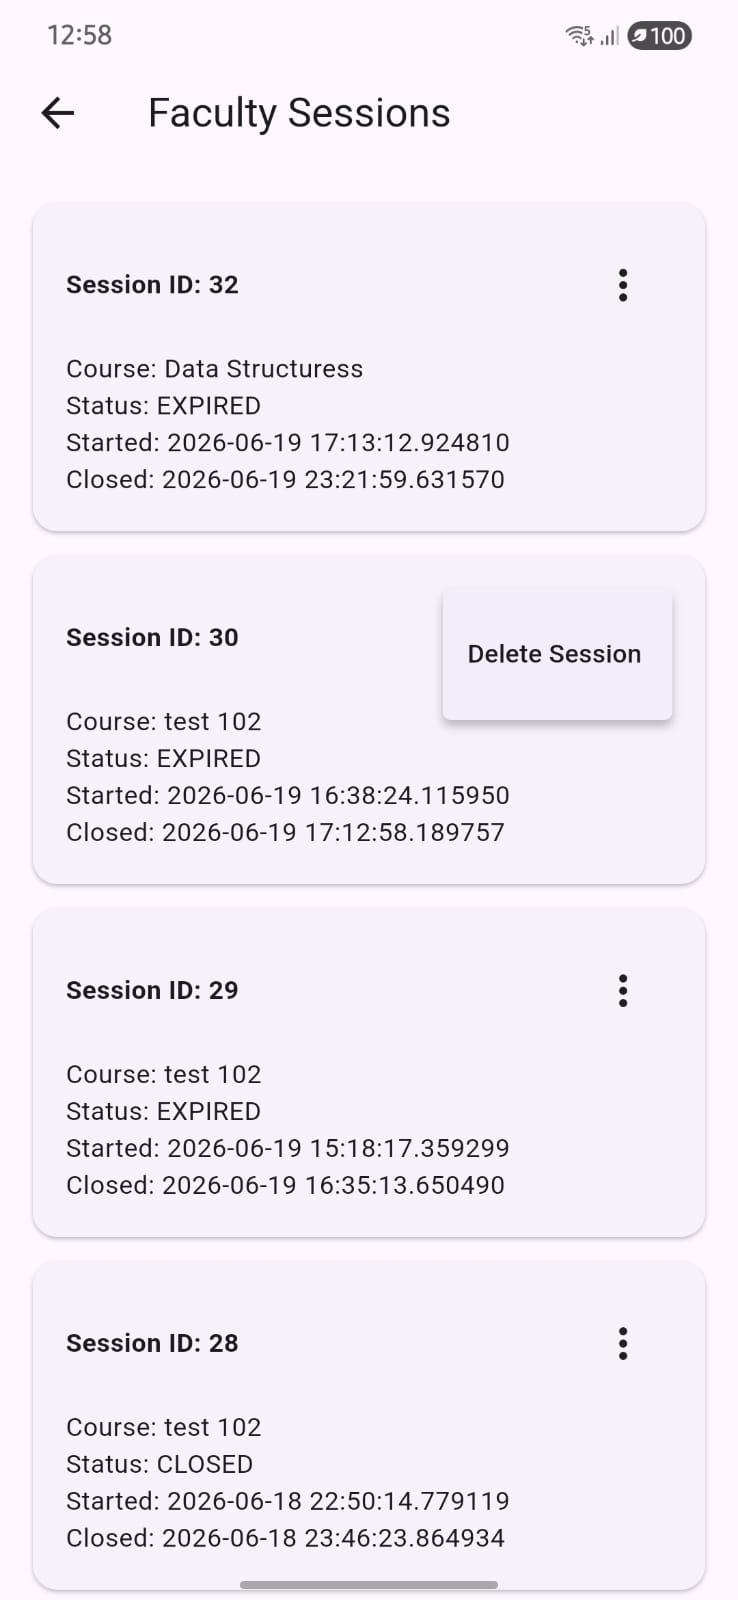
\includegraphics[width=0.7\textwidth]{images/screenshots/faculty/FAC_11_delete_session_option.jpeg}
    \caption{Faculty: Delete Session Option}
    \label{fig:appD-fac-11}
\end{figure}

\begin{figure}[htbp]
    \centering
    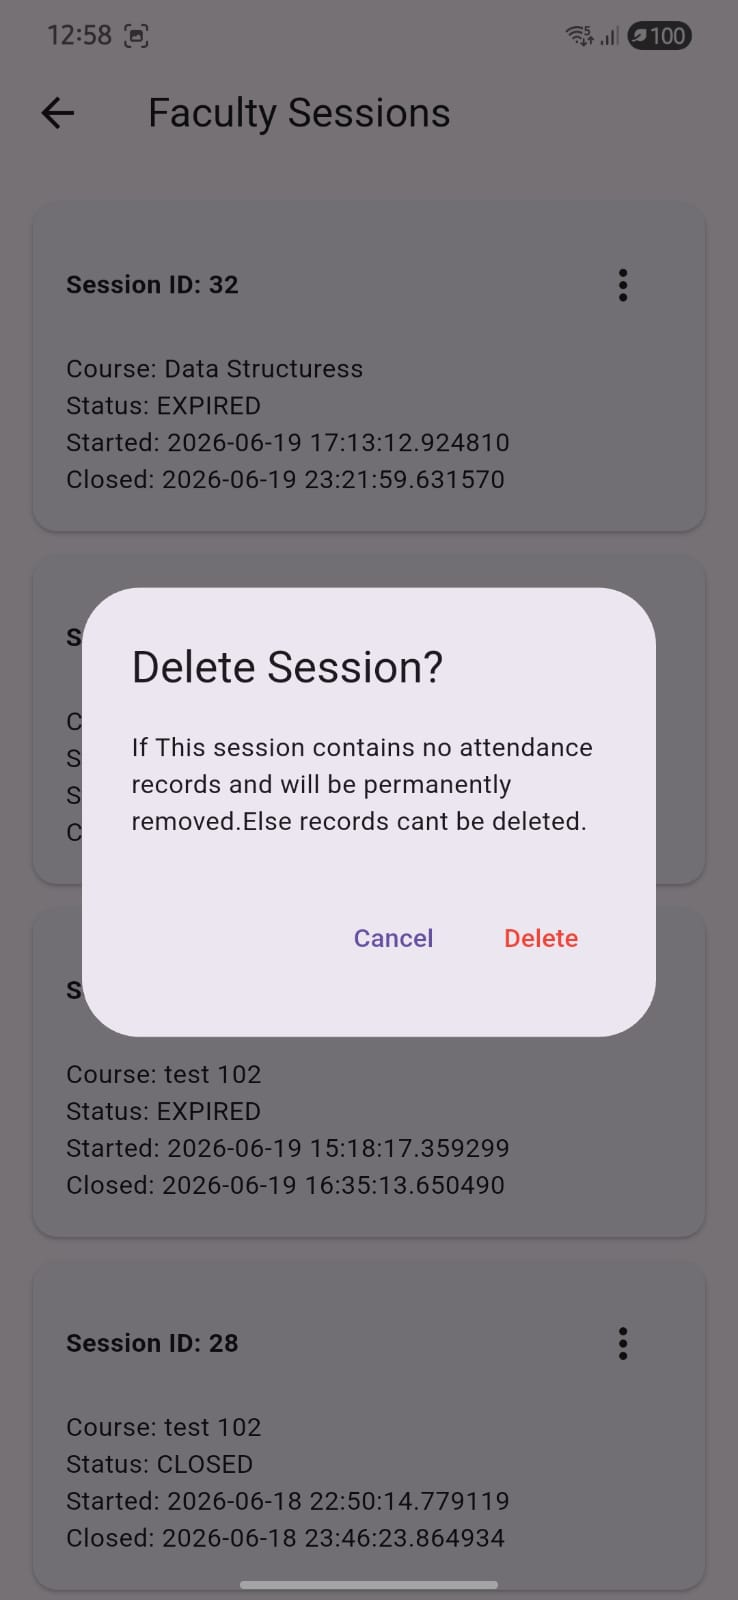
\includegraphics[width=0.7\textwidth]{images/screenshots/faculty/FAC_12_delete_session_confirmation.jpeg}
    \caption{Faculty: Delete Session Confirmation}
    \label{fig:appD-fac-12}
\end{figure}

\begin{figure}[htbp]
    \centering
    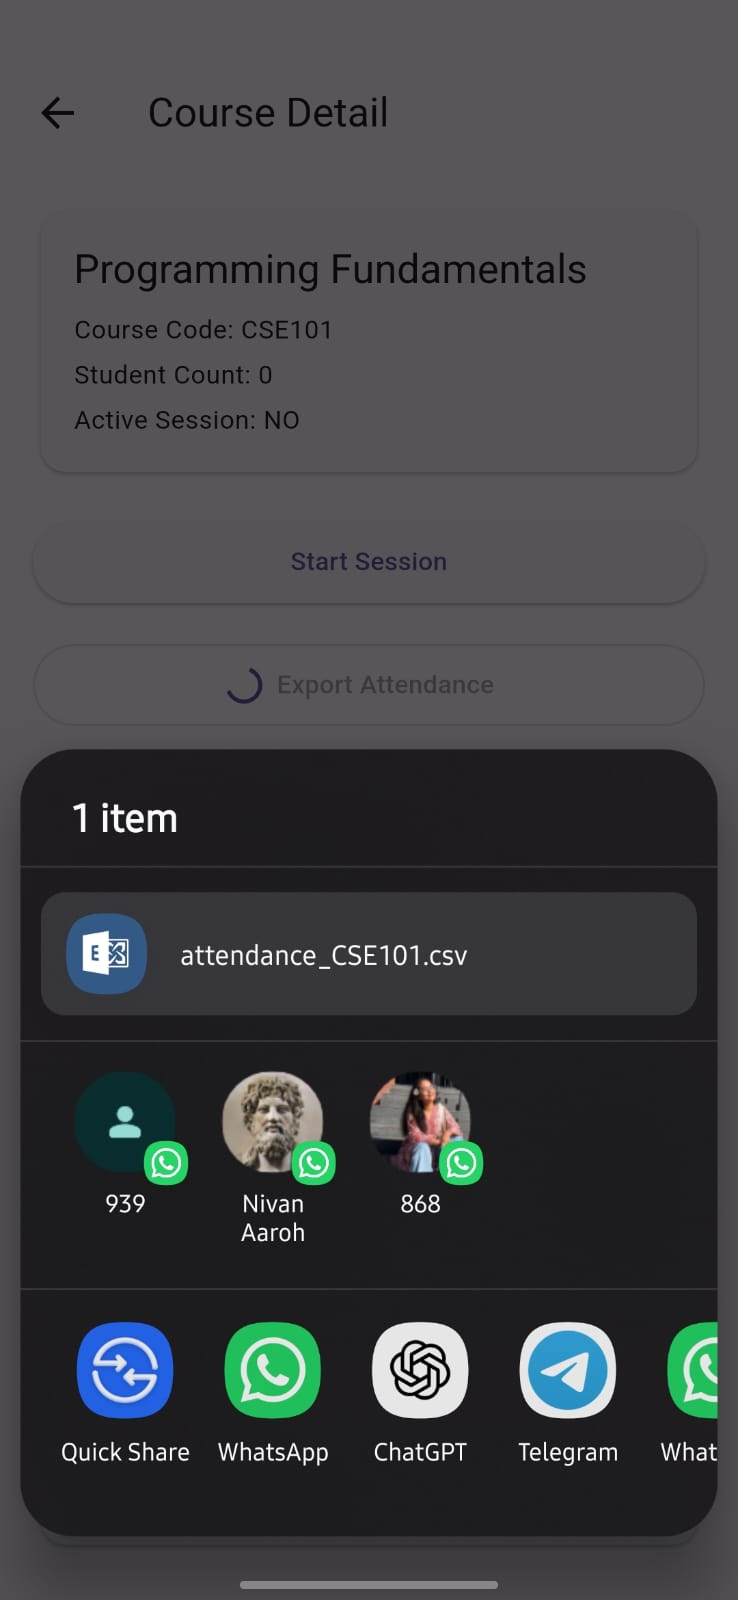
\includegraphics[width=0.7\textwidth]{images/screenshots/faculty/FAC_13_export_attendance_csv.jpeg}
    \caption{Faculty: Export Attendance to CSV}
    \label{fig:appD-fac-13}
\end{figure}

\section{Student Screenshots}
\label{app:screenshots-student}

\begin{figure}[htbp]
    \centering
    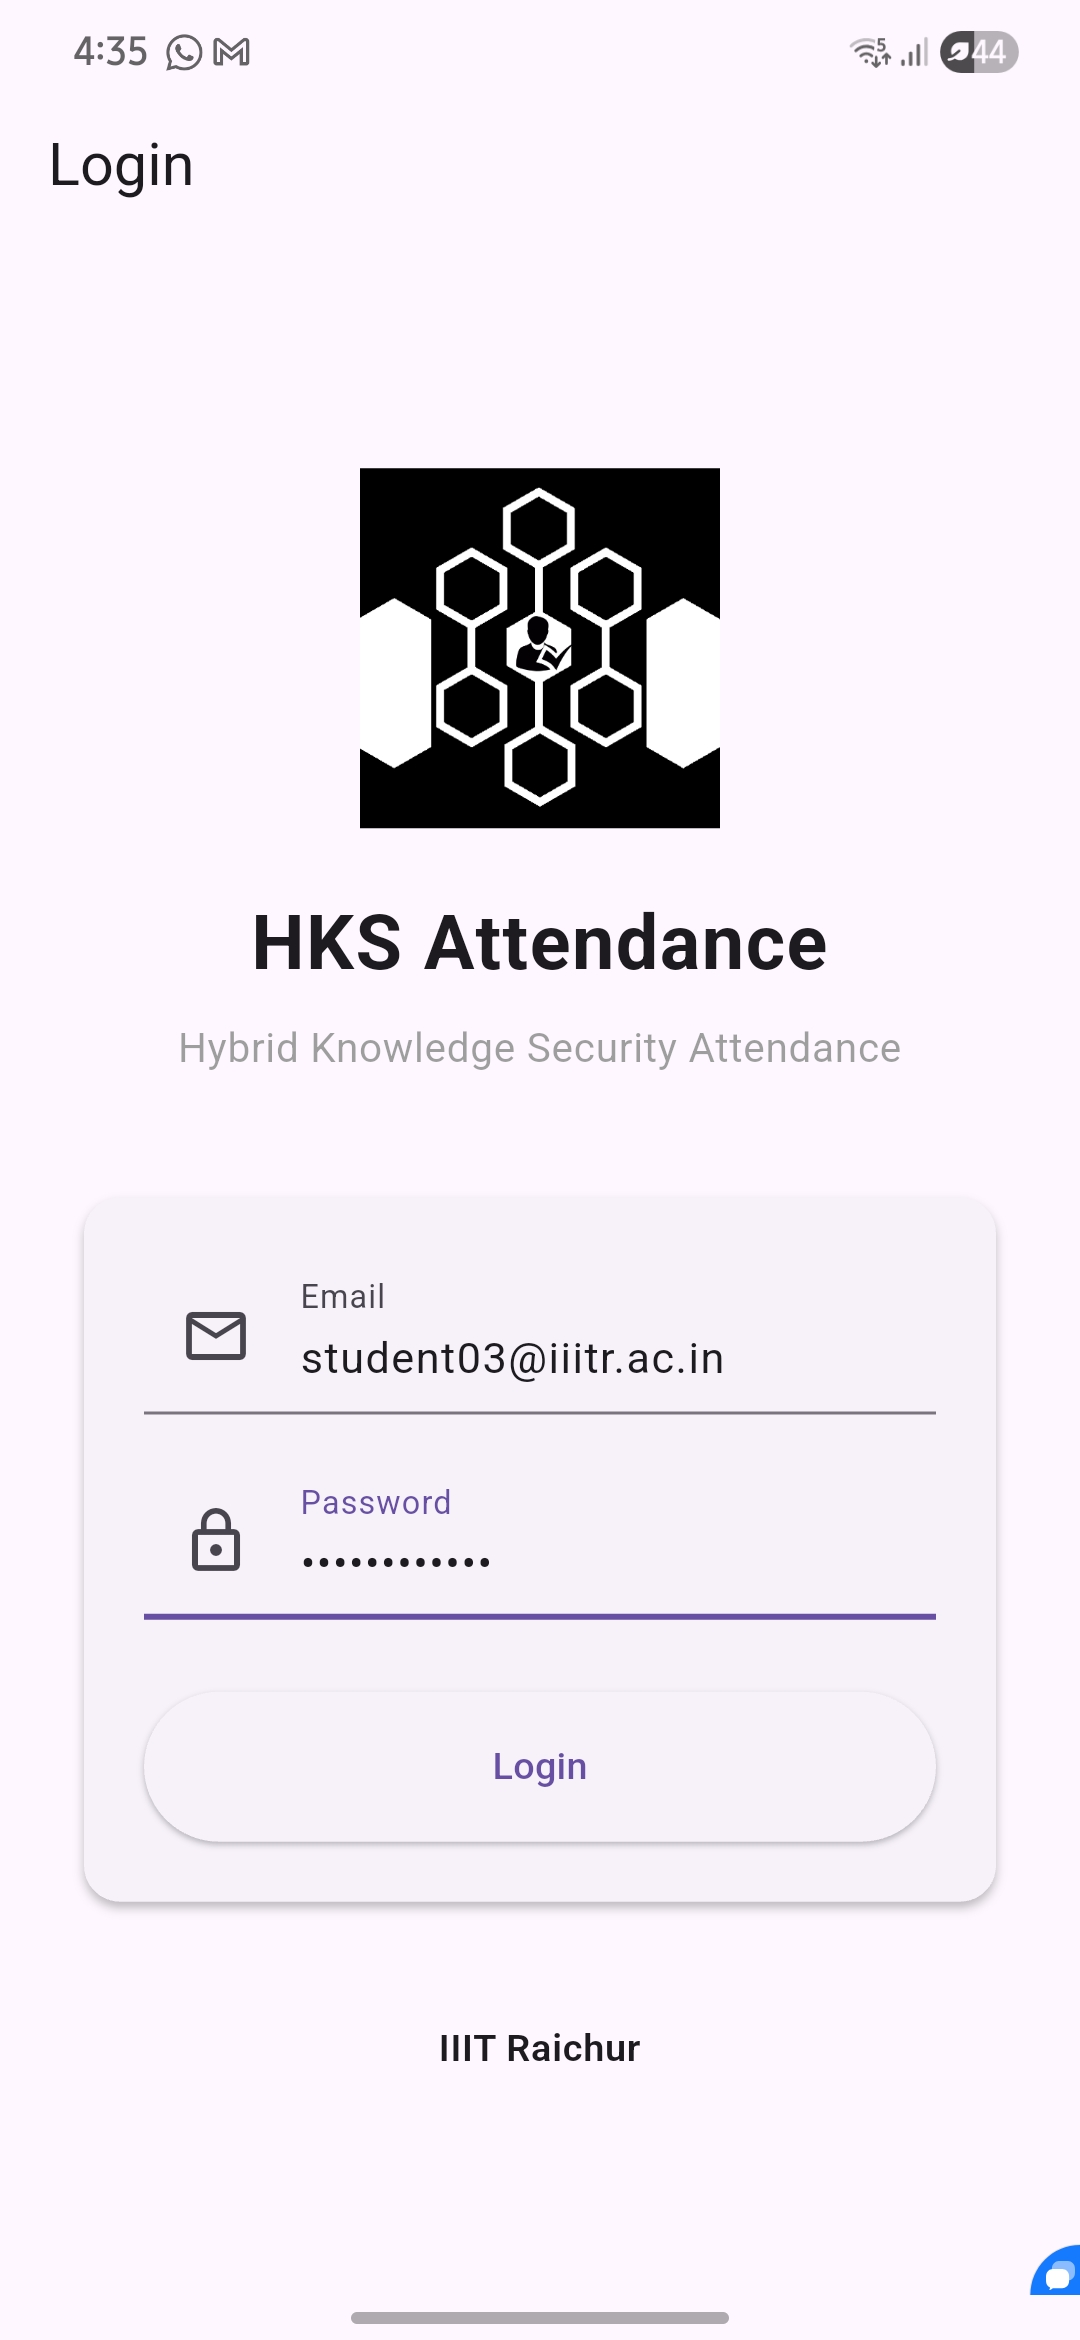
\includegraphics[width=0.7\textwidth]{images/screenshots/student/STU_01_login_screen.jpeg}
    \caption{Student: Login Screen}
    \label{fig:appD-stu-01}
\end{figure}

\begin{figure}[htbp]
    \centering
    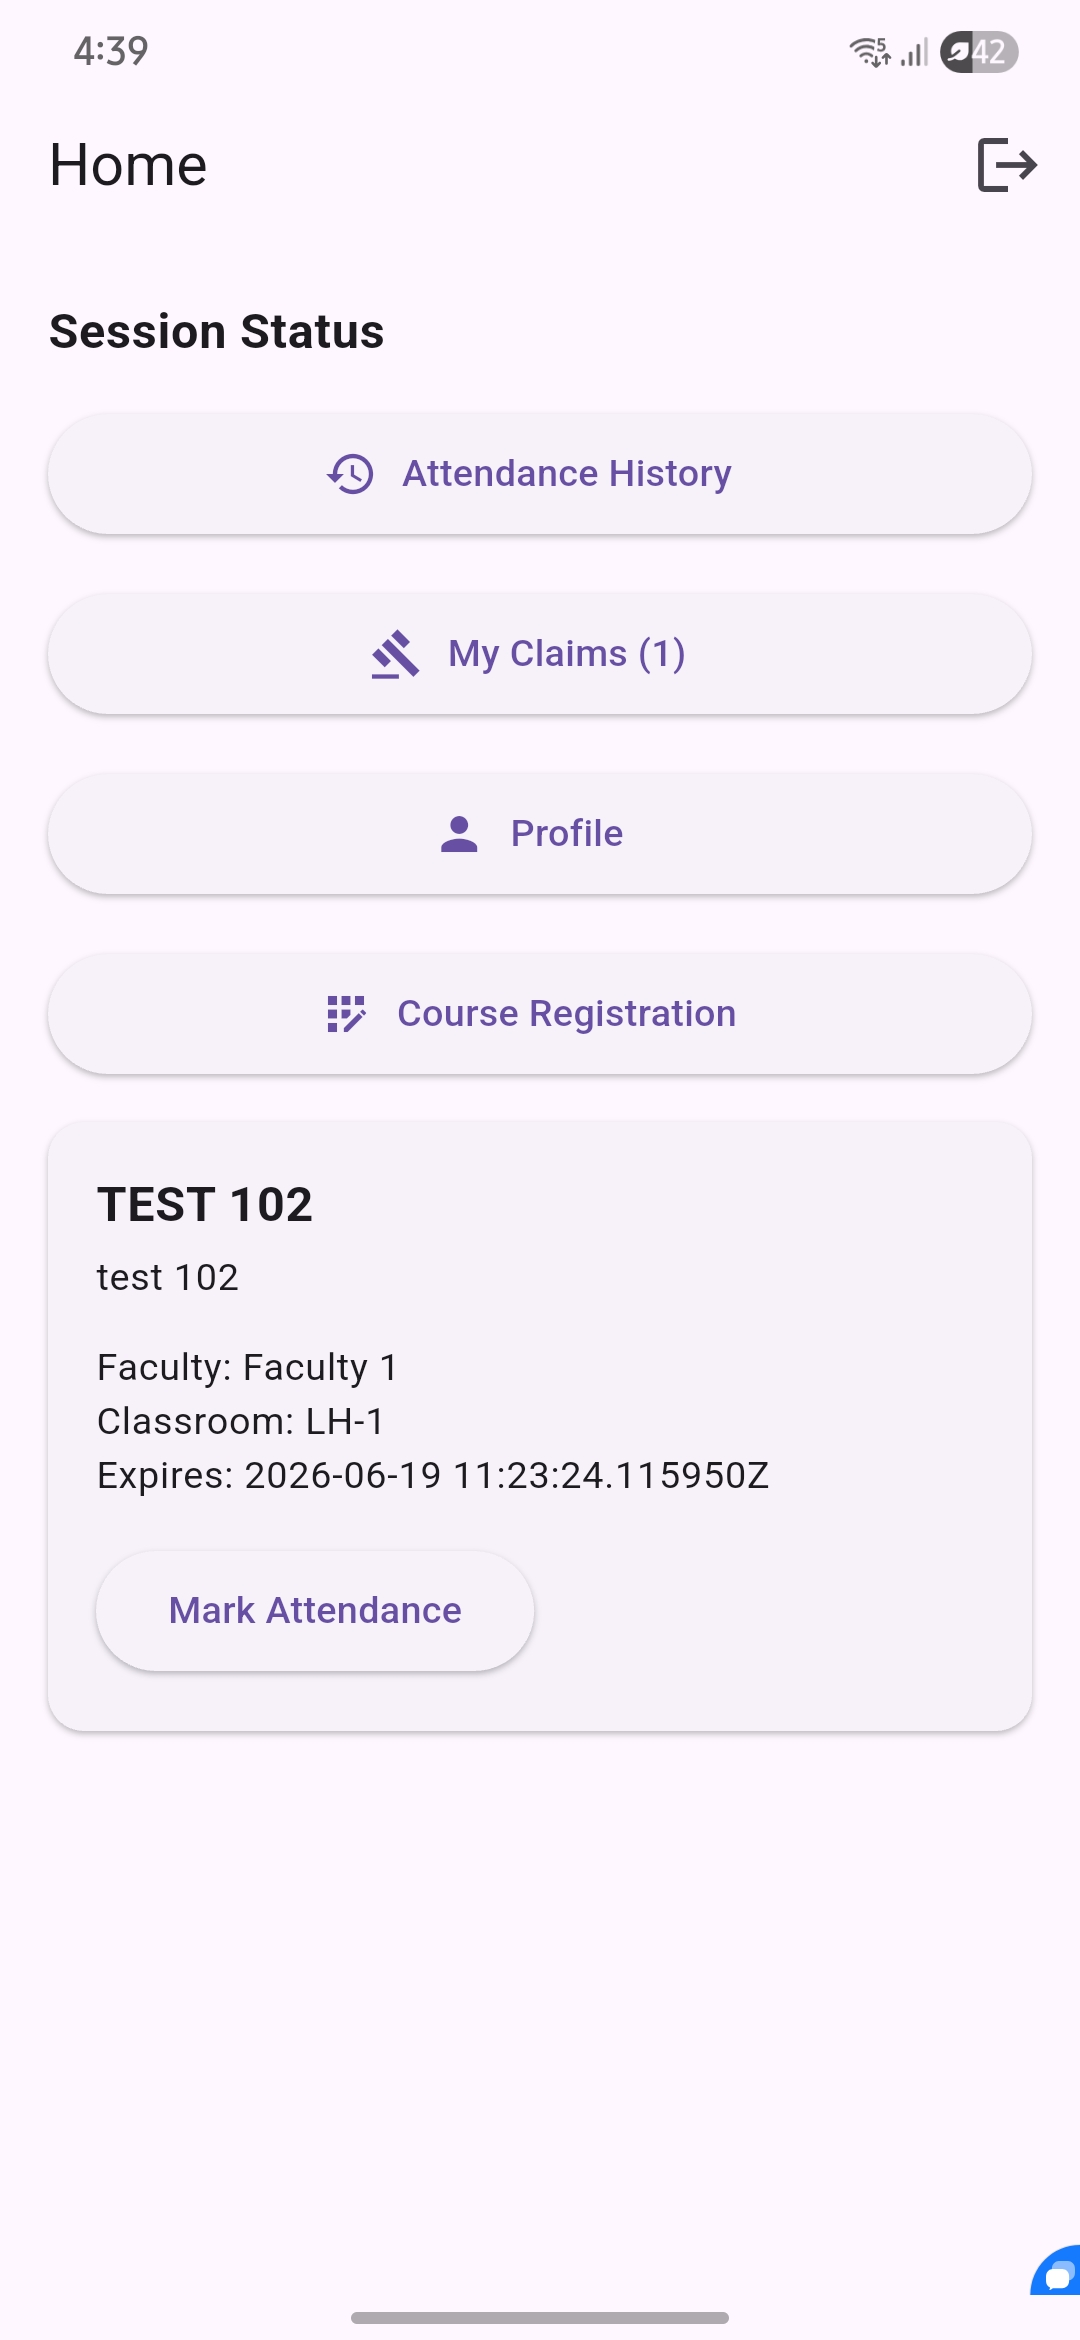
\includegraphics[width=0.7\textwidth]{images/screenshots/student/STU_02_active_session_available.jpeg}
    \caption{Student: Active Session Available}
    \label{fig:appD-stu-02}
\end{figure}

\begin{figure}[htbp]
    \centering
    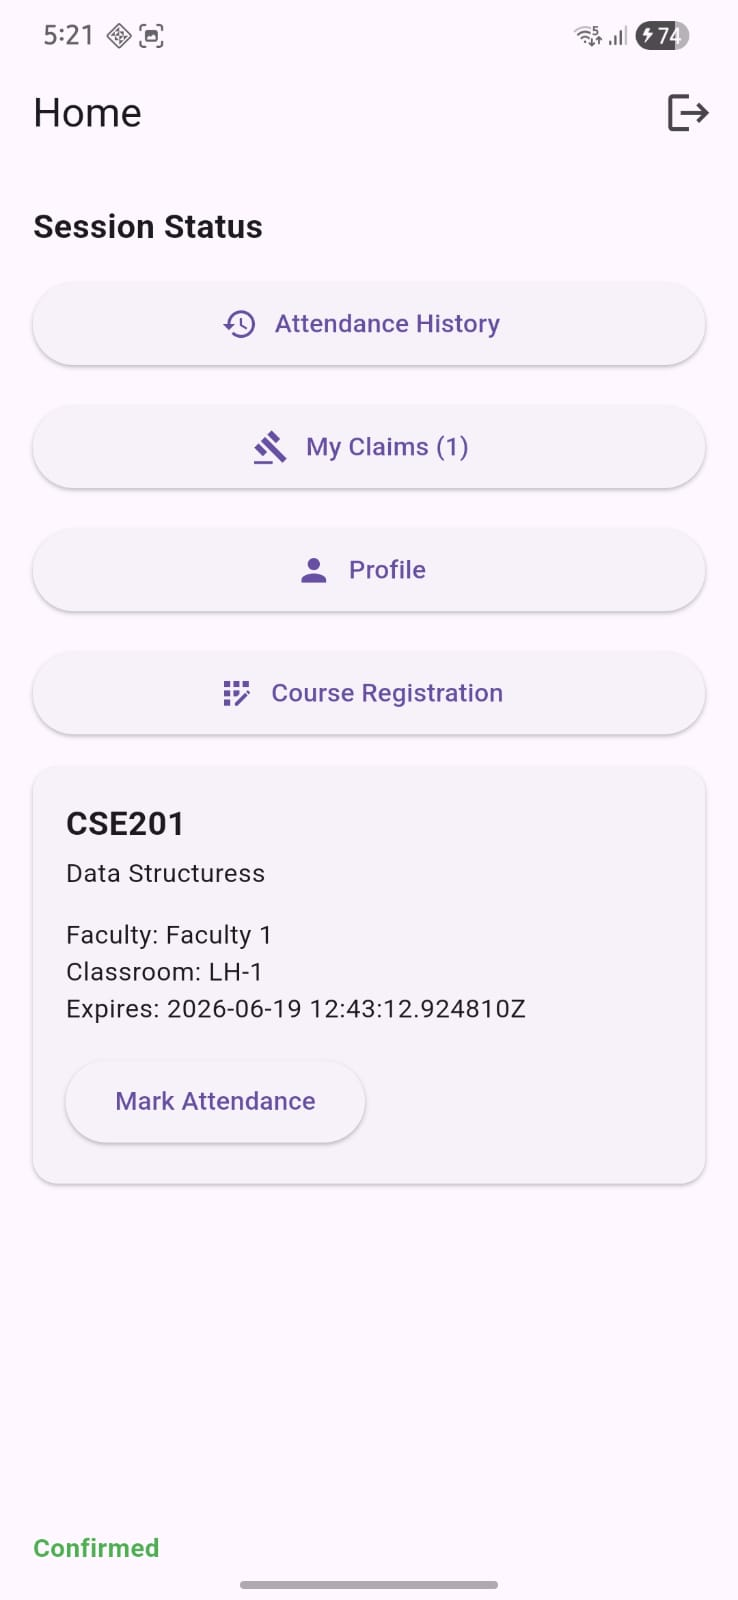
\includegraphics[width=0.7\textwidth]{images/screenshots/student/STU_03_attendance_confirmed.jpeg}
    \caption{Student: Attendance Confirmed}
    \label{fig:appD-stu-03}
\end{figure}

\begin{figure}[htbp]
    \centering
    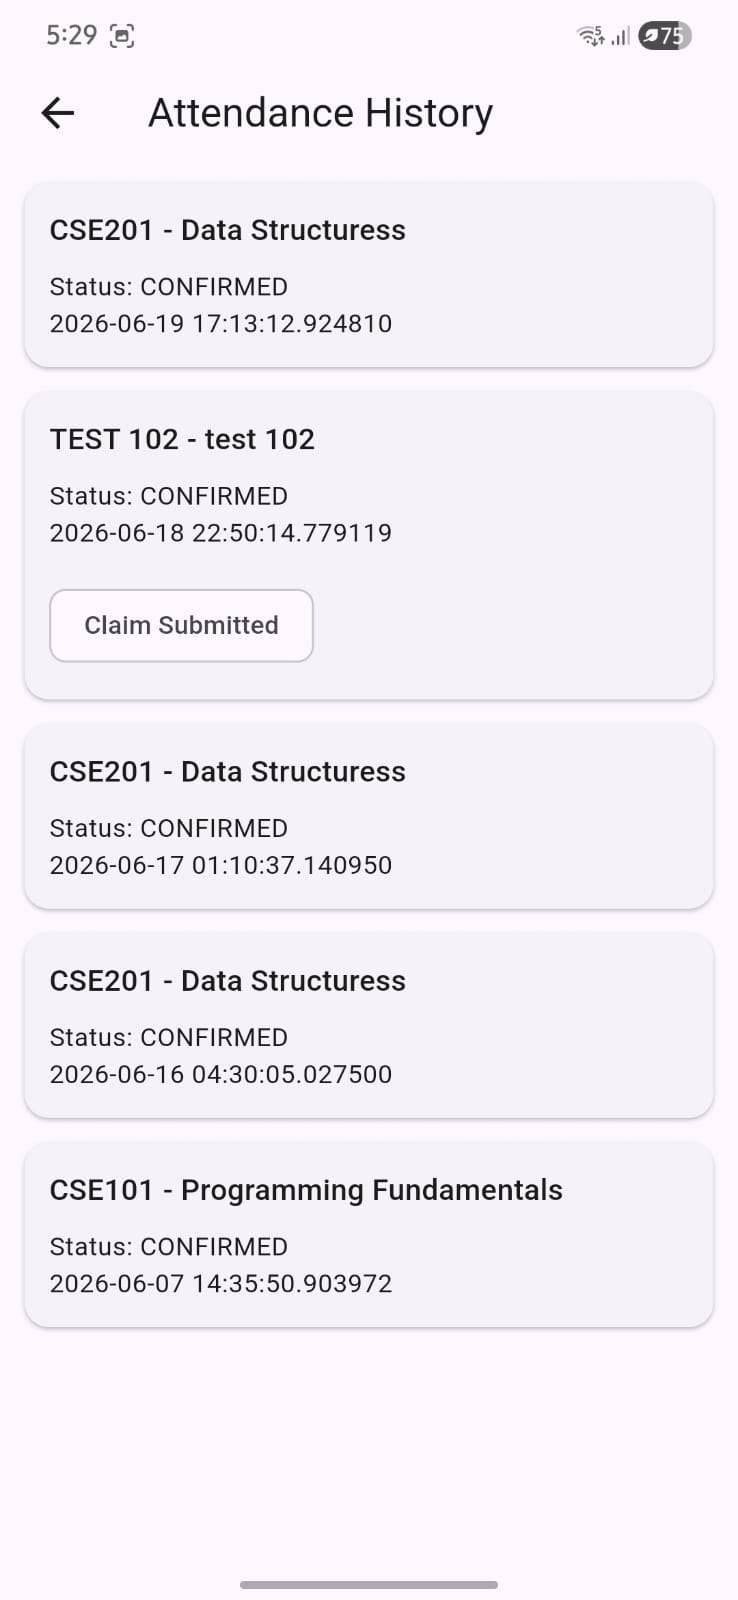
\includegraphics[width=0.7\textwidth]{images/screenshots/student/STU_04_attendance_history.jpeg}
    \caption{Student: Attendance History}
    \label{fig:appD-stu-04}
\end{figure}

\begin{figure}[htbp]
    \centering
    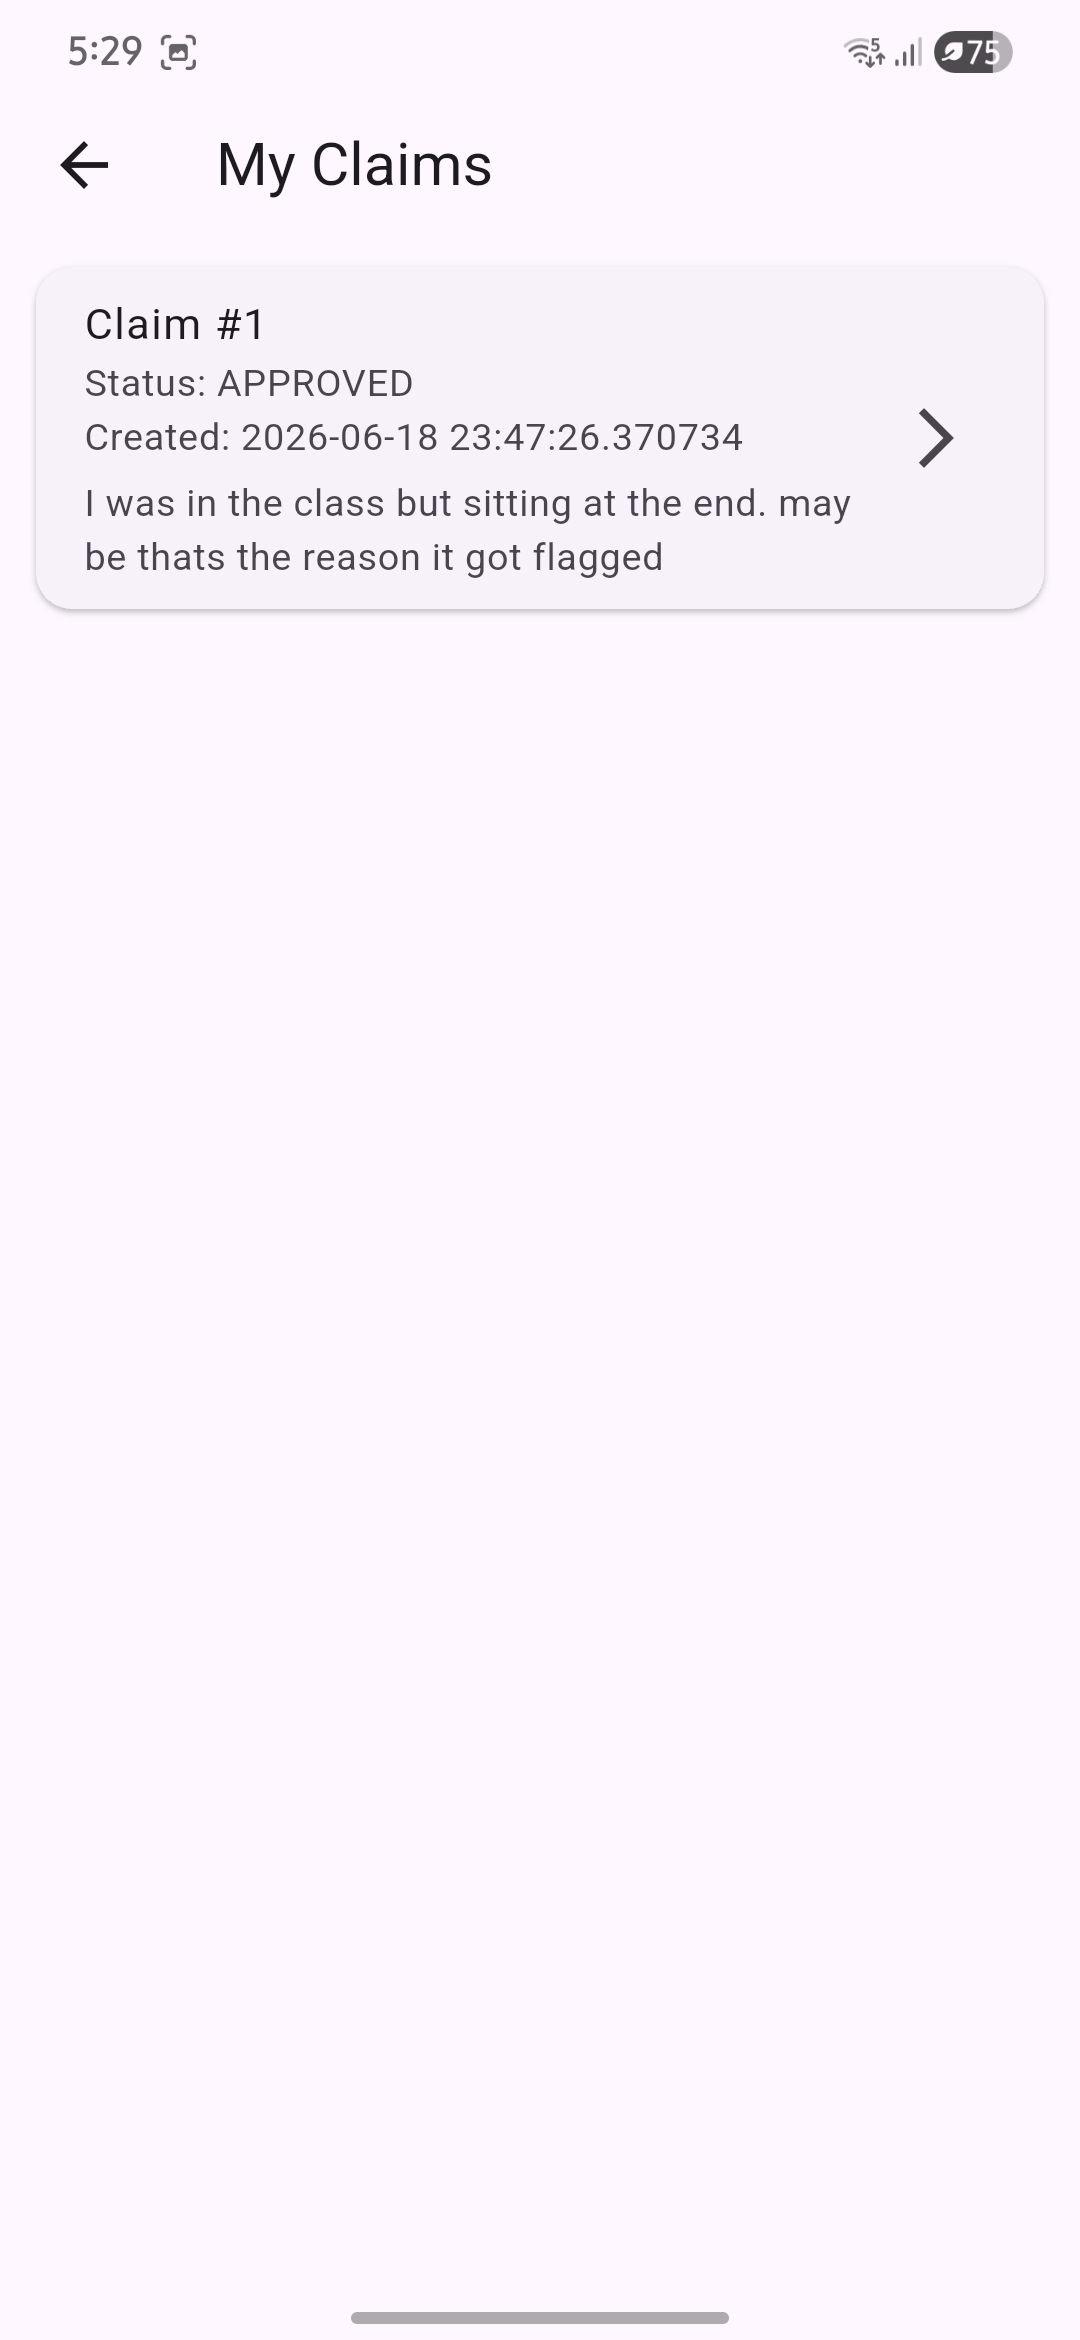
\includegraphics[width=0.7\textwidth]{images/screenshots/student/STU_05_my_claims.jpeg}
    \caption{Student: My Claims}
    \label{fig:appD-stu-05}
\end{figure}

\begin{figure}[htbp]
    \centering
    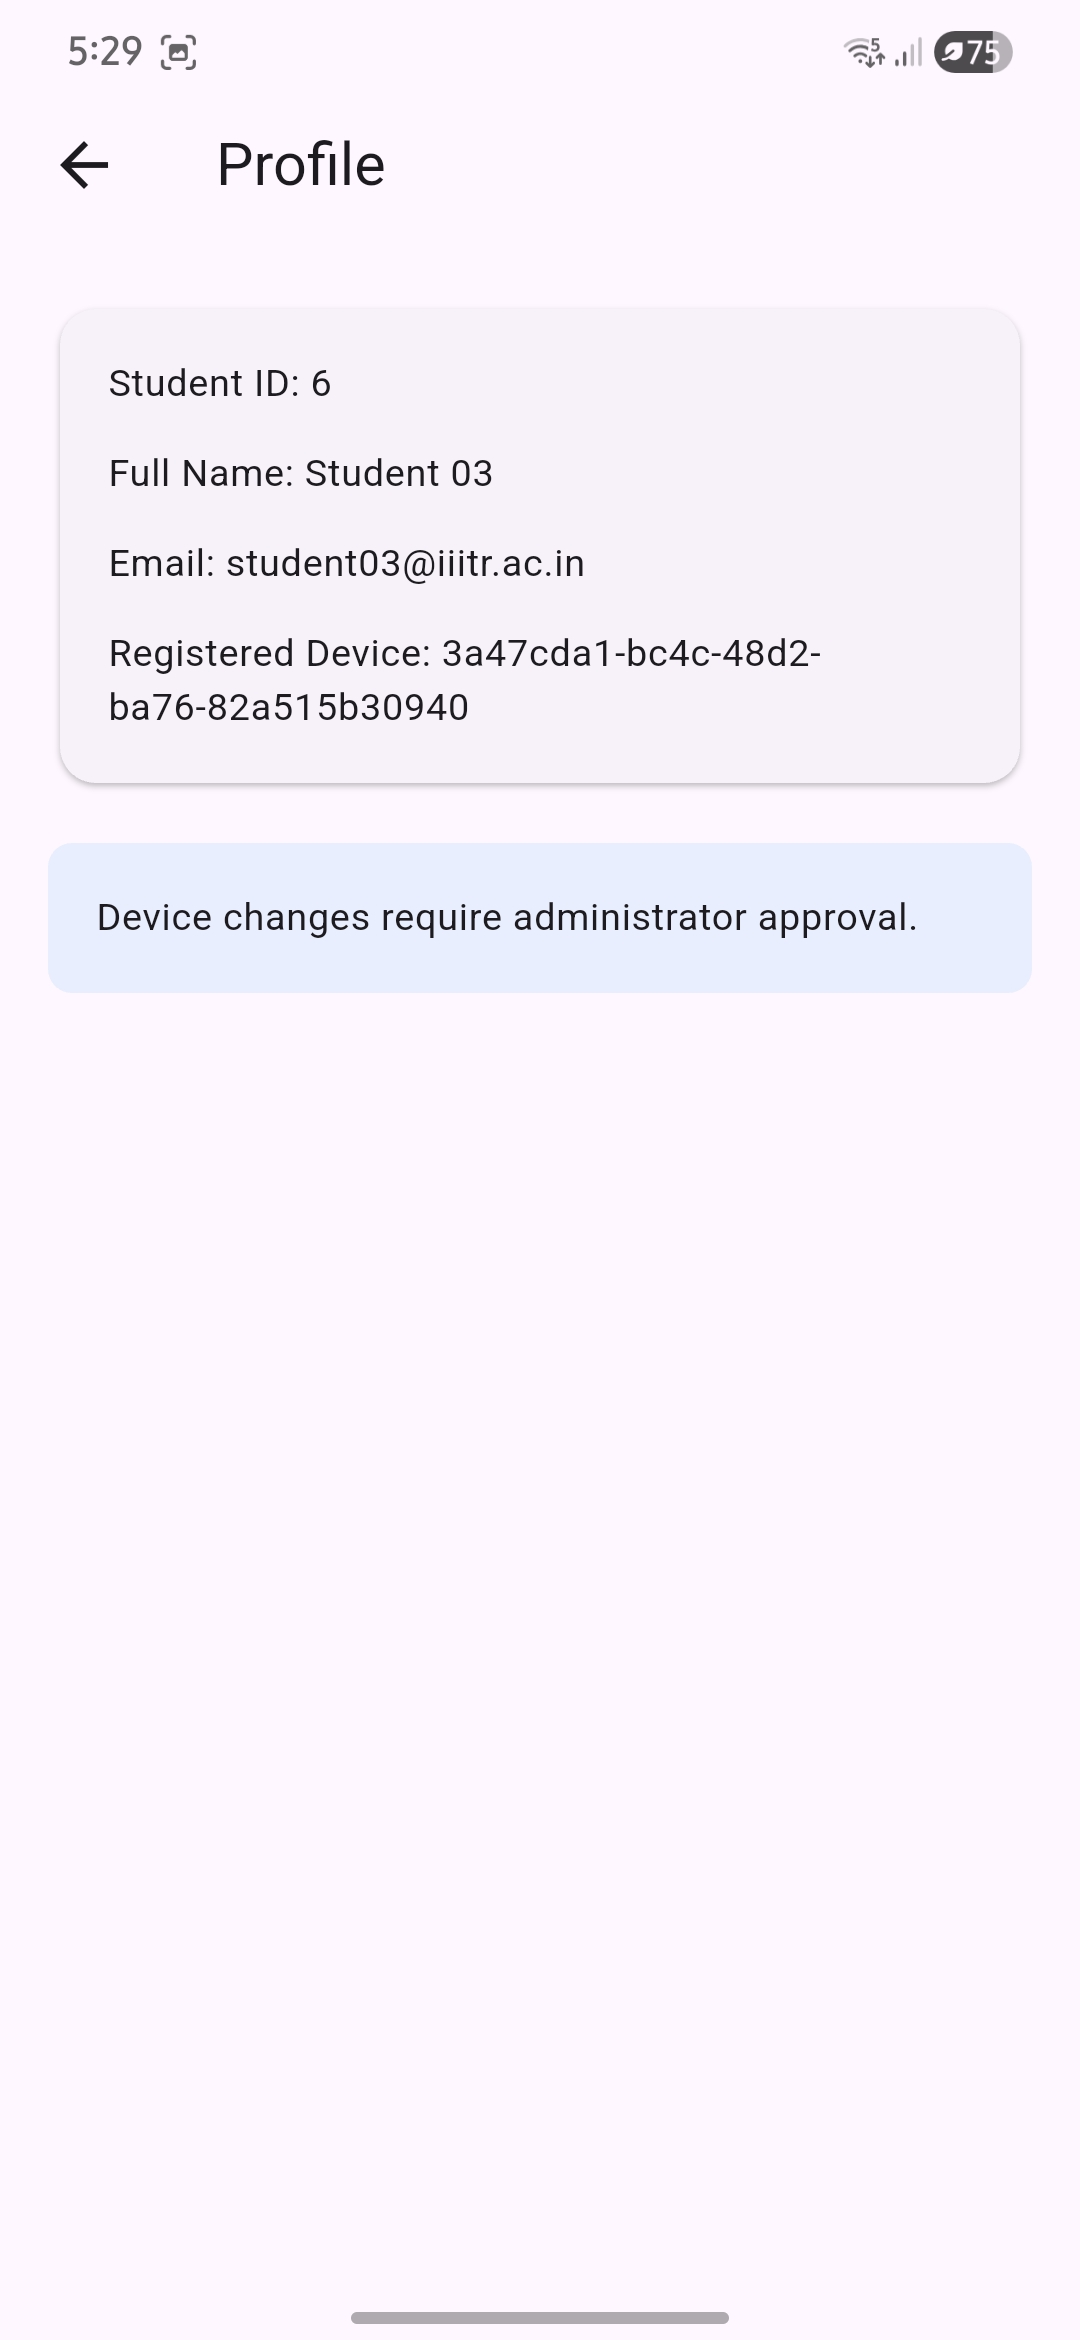
\includegraphics[width=0.7\textwidth]{images/screenshots/student/STU_06_student_profile.jpeg}
    \caption{Student: Profile}
    \label{fig:appD-stu-06}
\end{figure}

\begin{figure}[htbp]
    \centering
    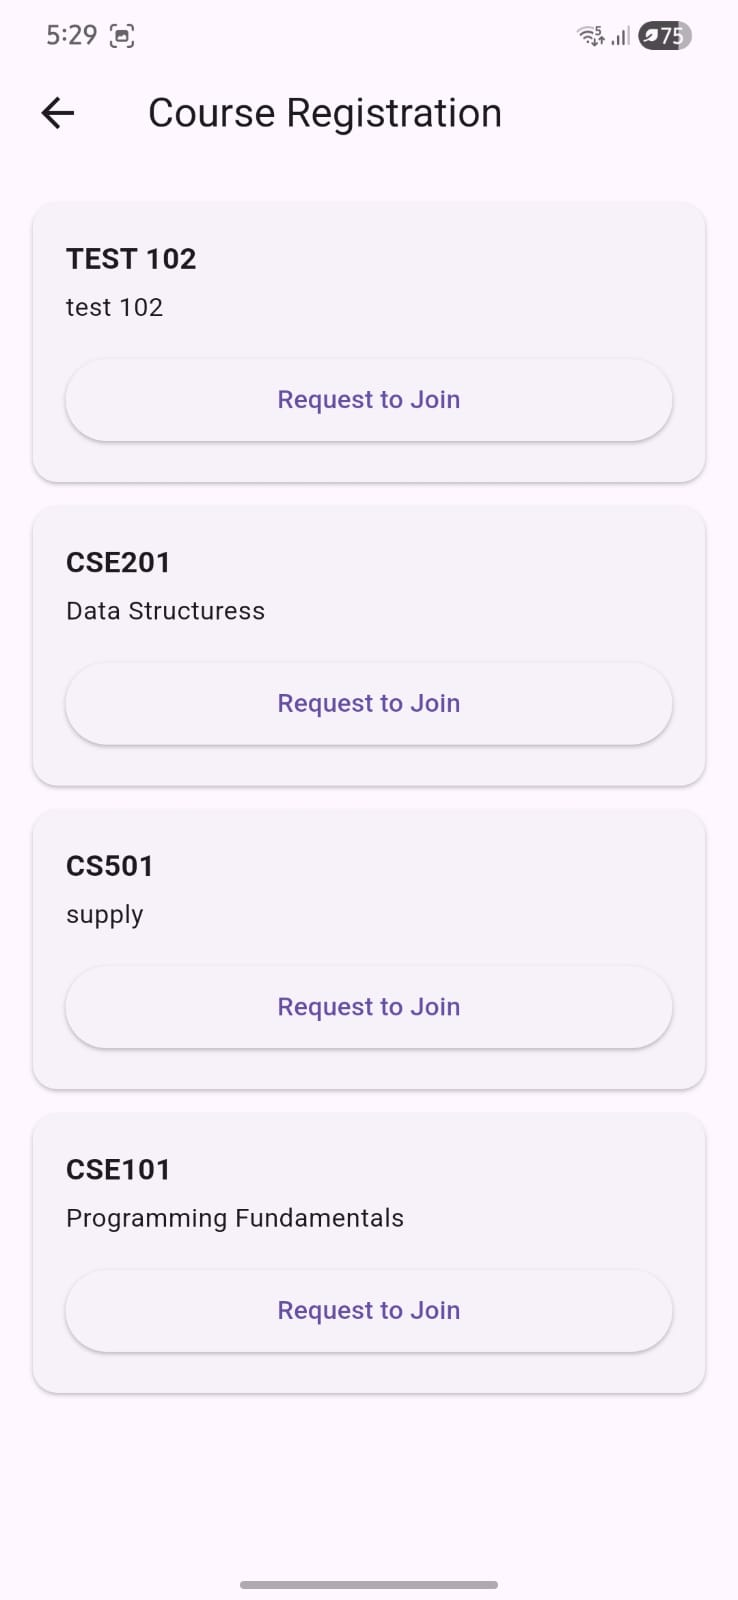
\includegraphics[width=0.7\textwidth]{images/screenshots/student/STU_07_course_registration.jpeg}
    \caption{Student: Course Registration}
    \label{fig:appD-stu-07}
\end{figure}

\begin{figure}[htbp]
    \centering
    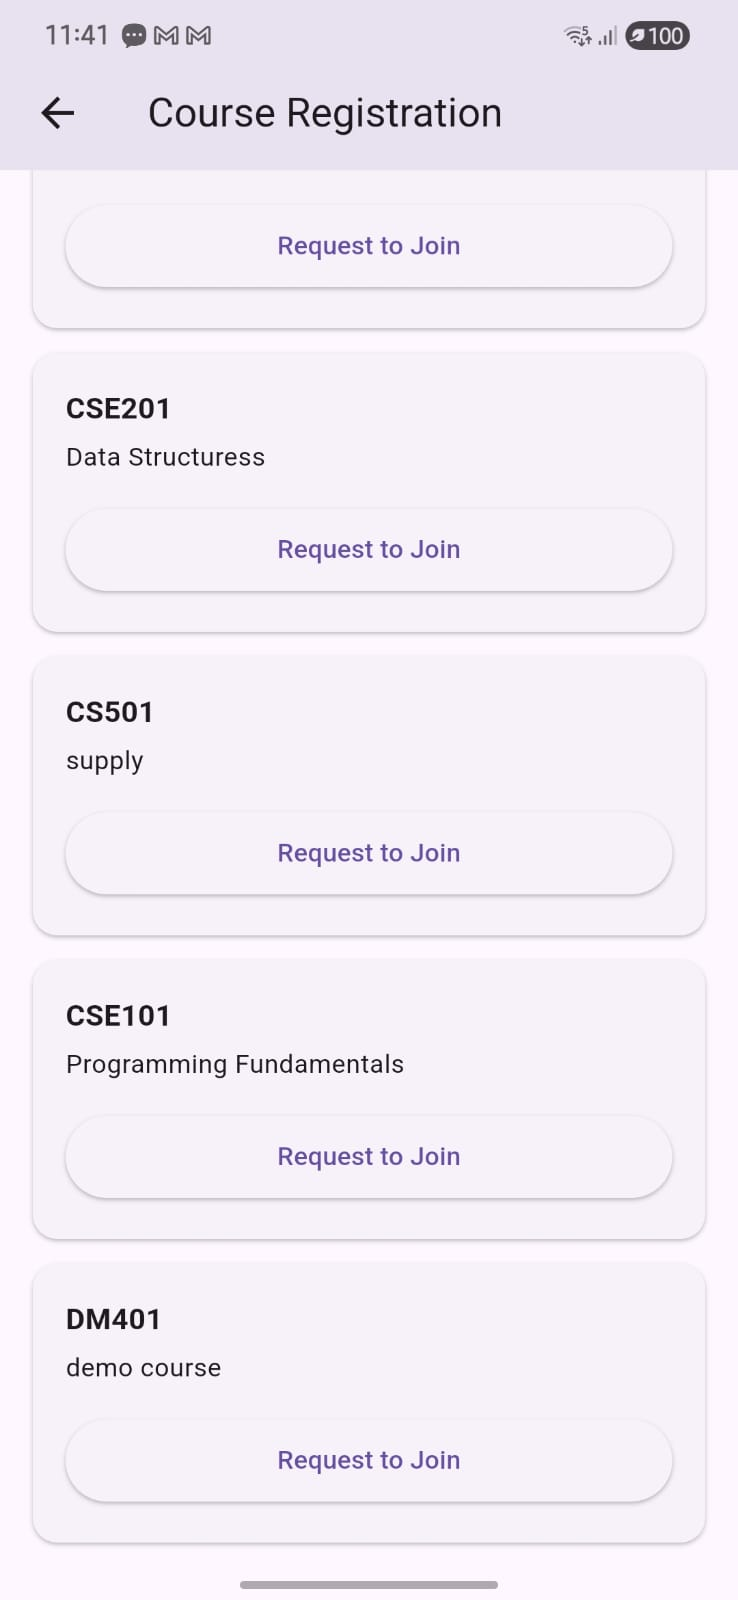
\includegraphics[width=0.7\textwidth]{images/screenshots/student/STU_08_course_registration_request.jpeg}
    \caption{Student: Course Registration Request Submitted}
    \label{fig:appD-stu-08}
\end{figure}

\section{Claims Screenshots}
\label{app:screenshots-claims}

\begin{figure}[htbp]
    \centering
    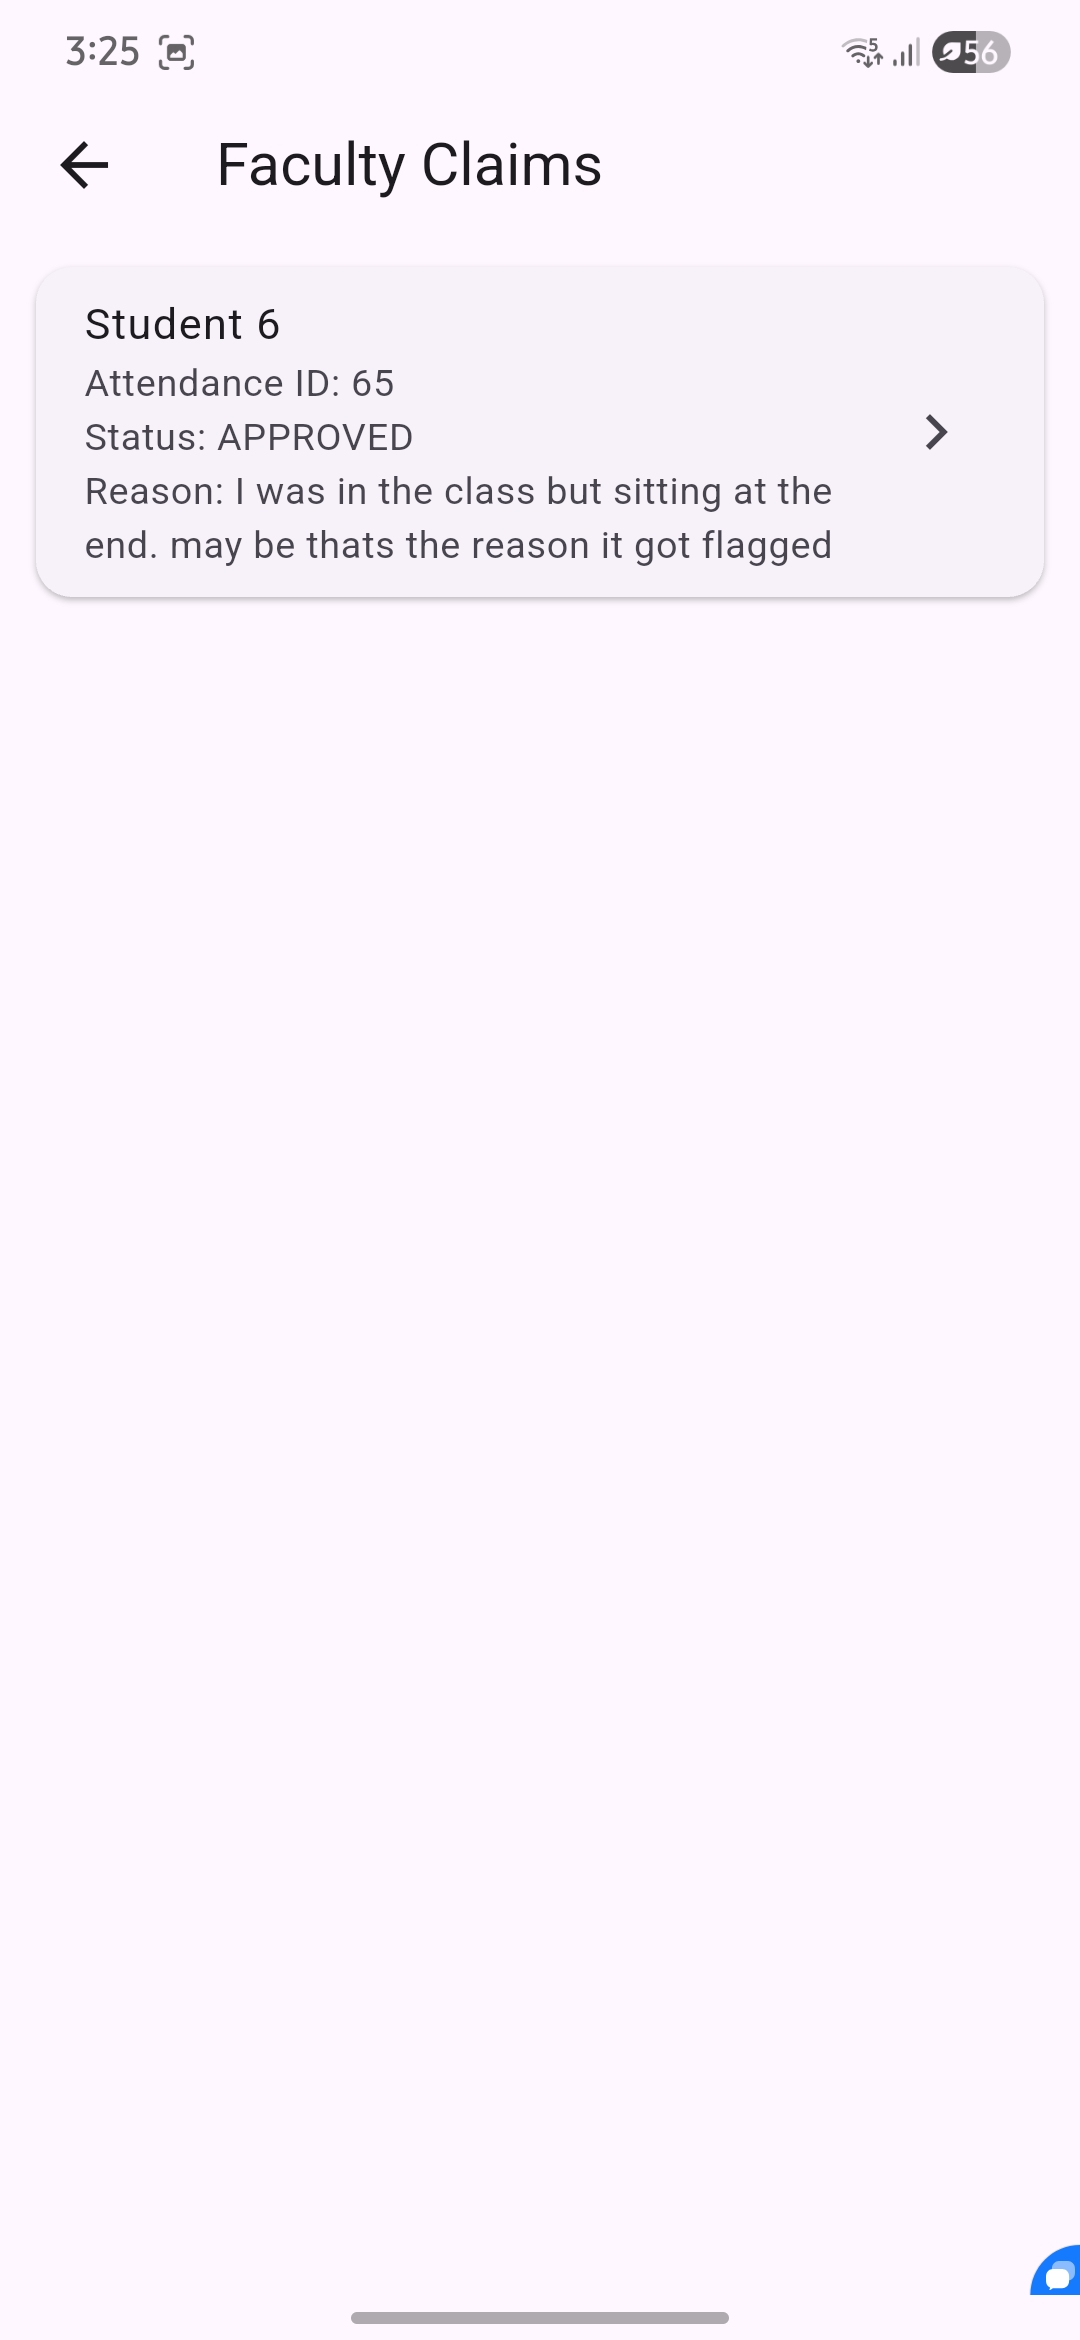
\includegraphics[width=0.7\textwidth]{images/screenshots/claims/CLAIM_01_claims_list.jpeg}
    \caption{Claims: Claims List}
    \label{fig:appD-claim-01}
\end{figure}

\begin{figure}[htbp]
    \centering
    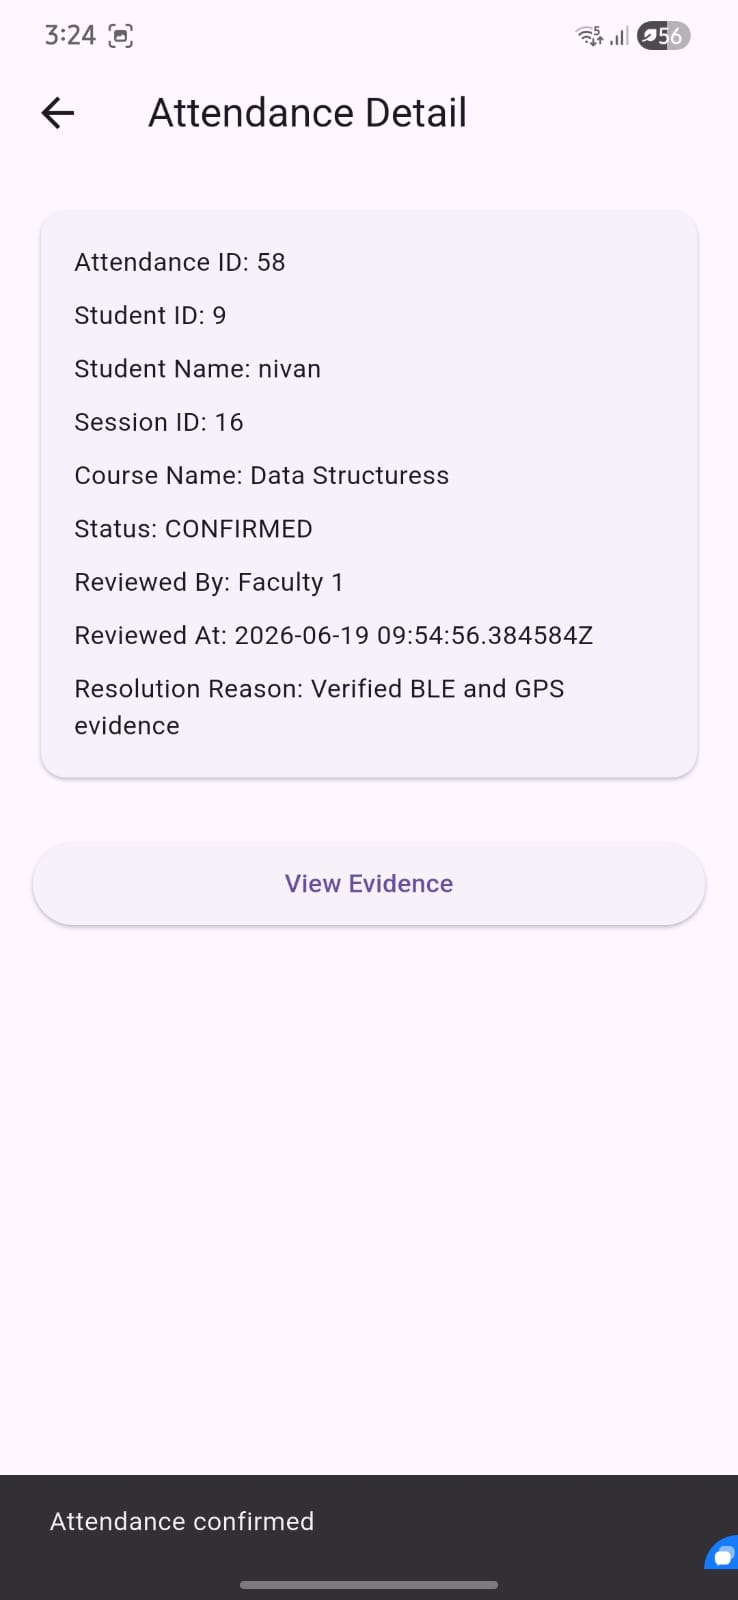
\includegraphics[width=0.7\textwidth]{images/screenshots/claims/CLAIM_02_claim_detail.jpeg}
    \caption{Claims: Claim Detail}
    \label{fig:appD-claim-02}
\end{figure}

\begin{figure}[htbp]
    \centering
    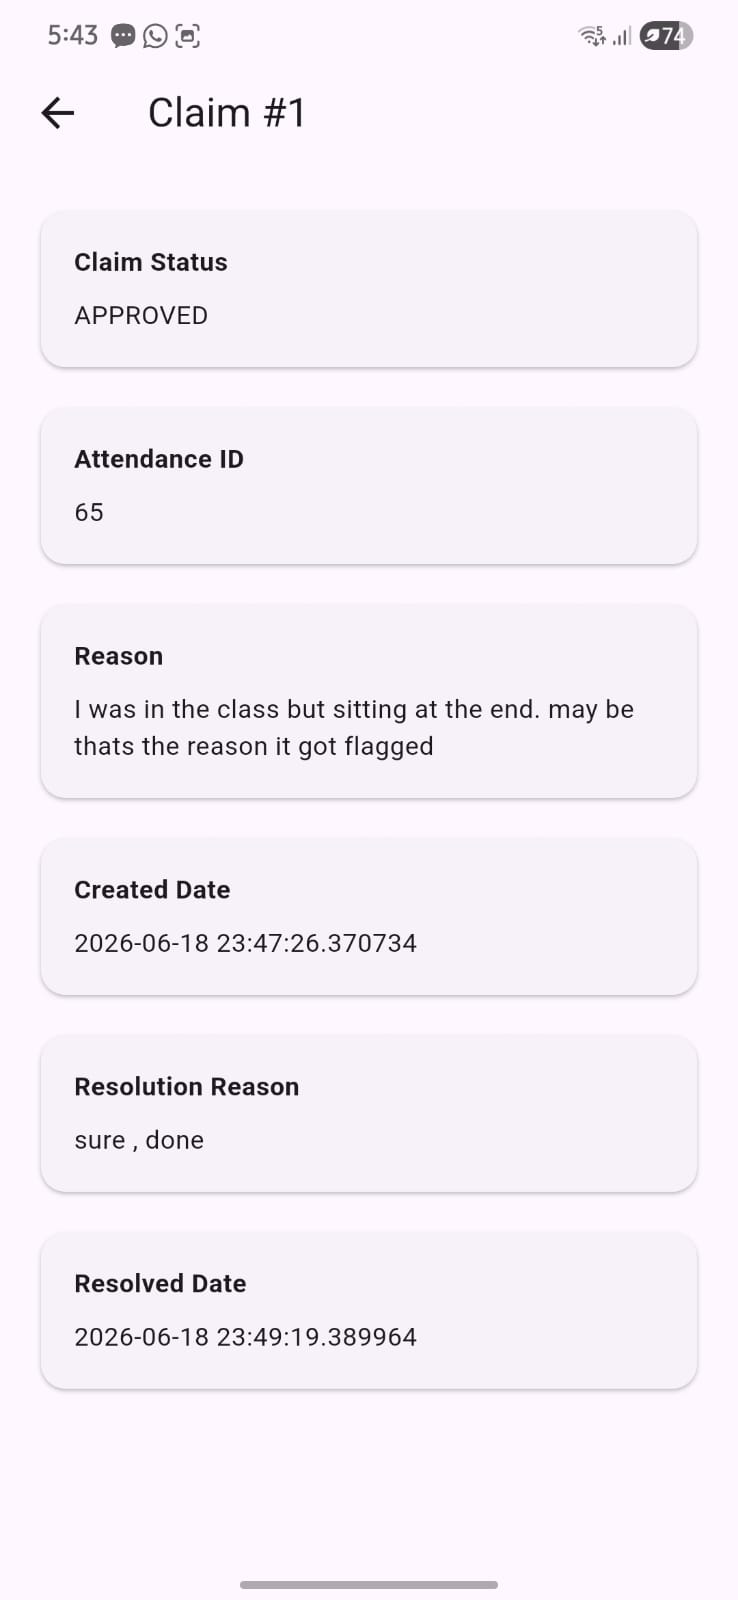
\includegraphics[width=0.7\textwidth]{images/screenshots/claims/CLAIM_03_approved_claim_detail.jpeg}
    \caption{Claims: Approved Claim Detail}
    \label{fig:appD-claim-03}
\end{figure}

\section{Attendance and Security Screenshots}
\label{app:screenshots-attendance-security}

\begin{figure}[htbp]
    \centering
    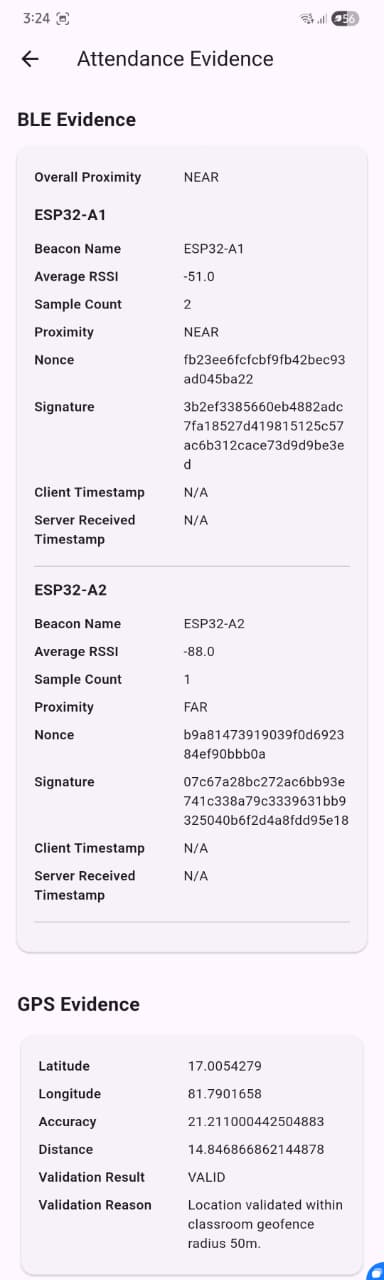
\includegraphics[width=0.7\textwidth]{images/screenshots/attendance/ATT_01_attendance_evidence.jpeg}
    \caption{Attendance: Submitted Evidence}
    \label{fig:appD-att-01}
\end{figure}

\begin{figure}[htbp]
    \centering
    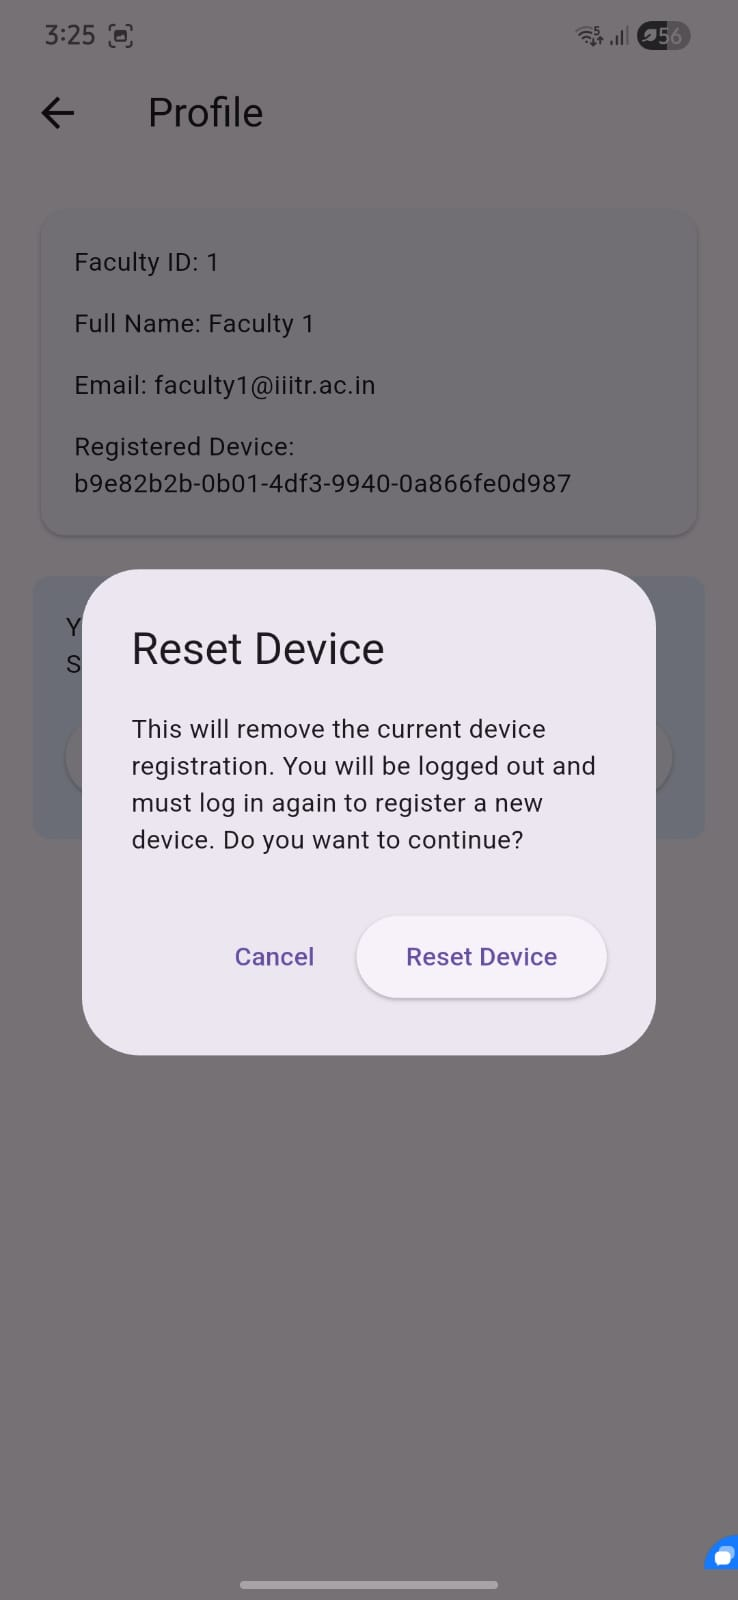
\includegraphics[width=0.7\textwidth]{images/screenshots/security/SEC_01_device_reset_confirmation.jpeg}
    \caption{Security: Device Reset Confirmation}
    \label{fig:appD-sec-01}
\end{figure}

\begin{figure}[htbp]
    \centering
    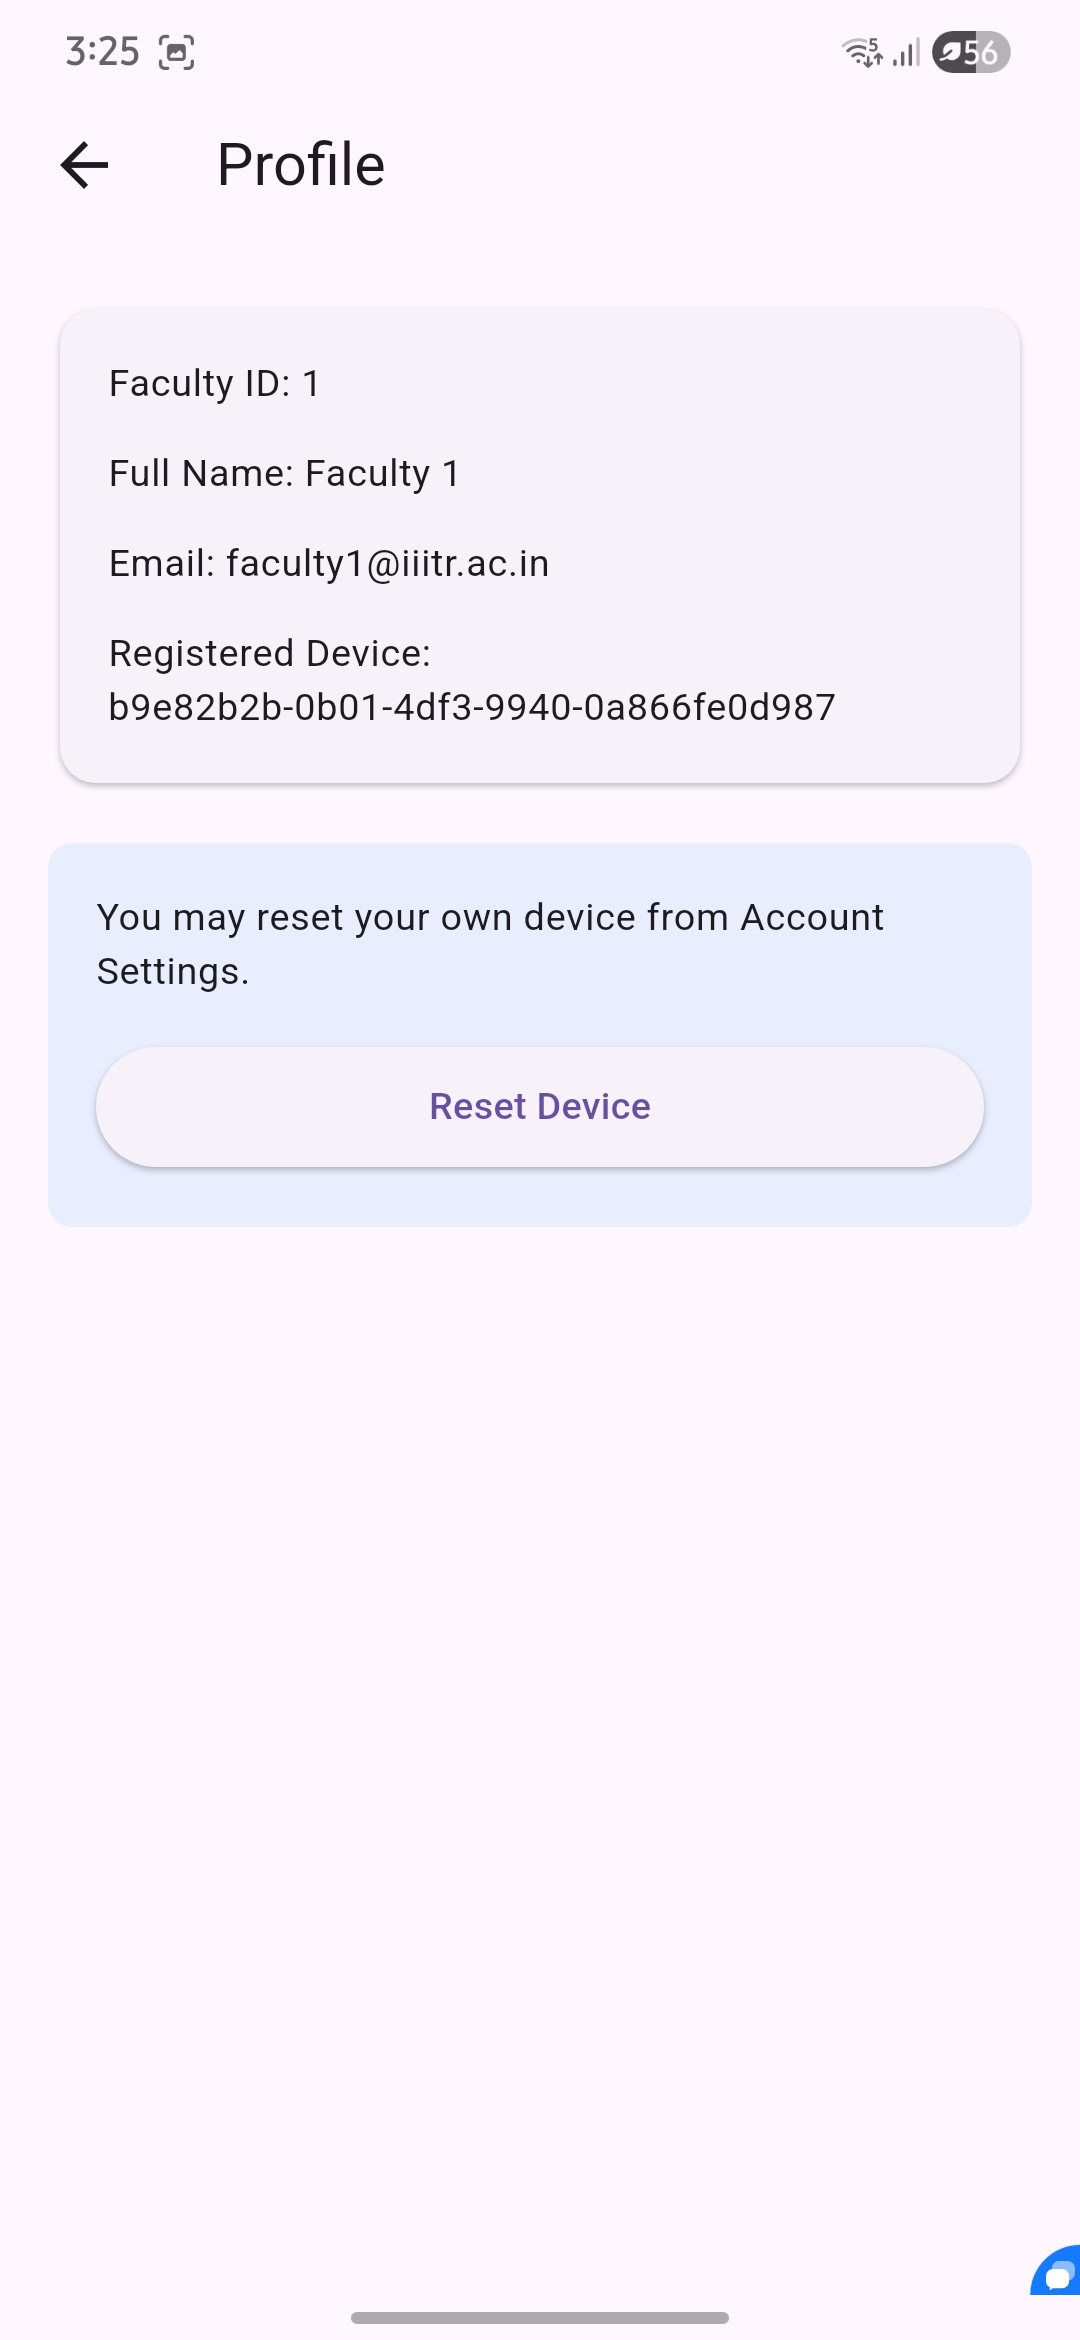
\includegraphics[width=0.7\textwidth]{images/screenshots/security/SEC_02_device_registered.jpeg}
    \caption{Security: Device Registered}
    \label{fig:appD-sec-02}
\end{figure}

\begin{figure}[htbp]
    \centering
    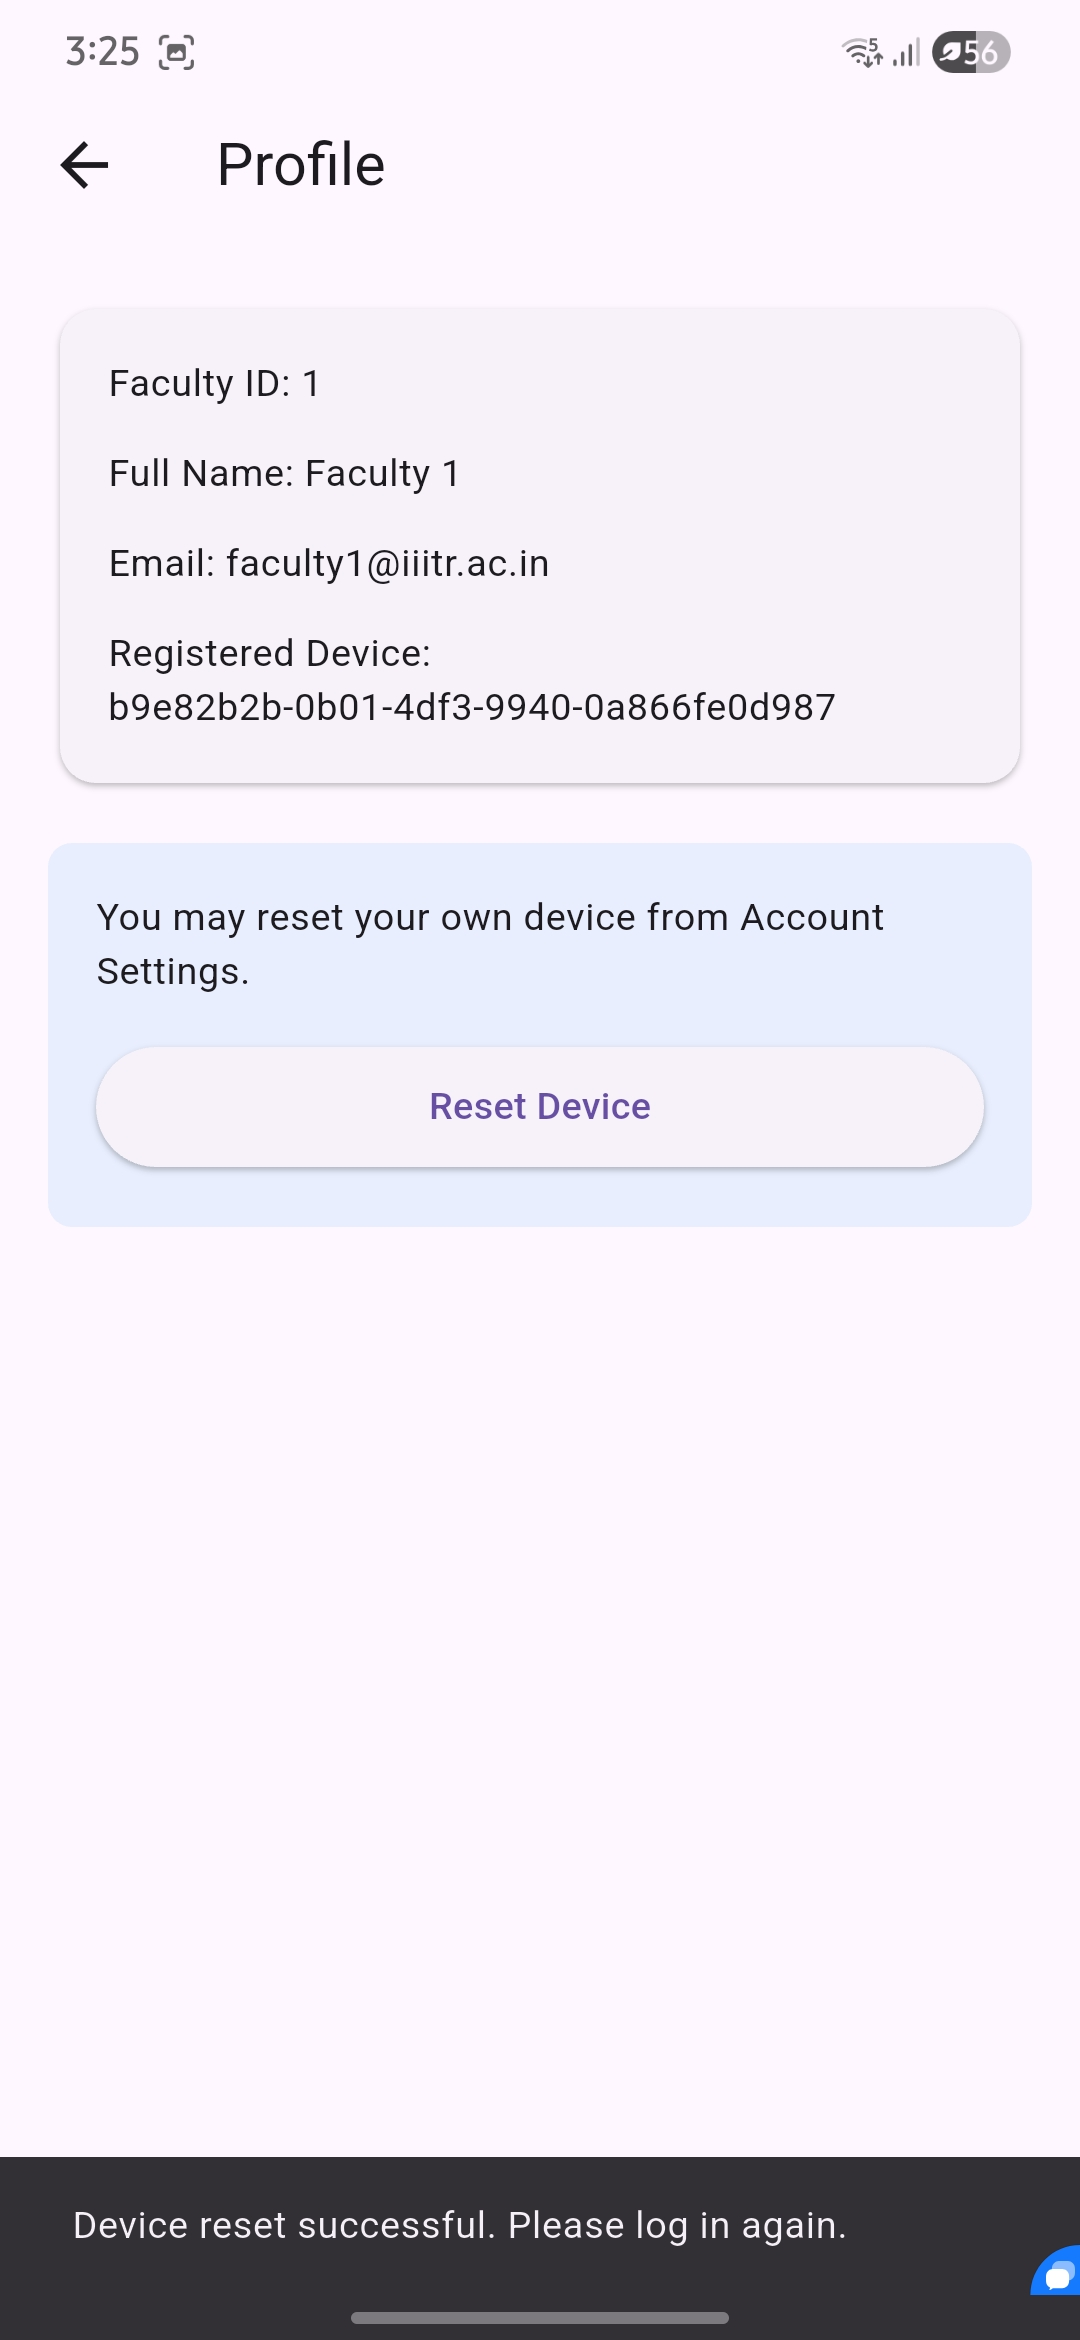
\includegraphics[width=0.7\textwidth]{images/screenshots/security/SEC_03_device_reset_success.jpeg}
    \caption{Security: Device Reset Success}
    \label{fig:appD-sec-03}
\end{figure}

\begin{figure}[htbp]
    \centering
    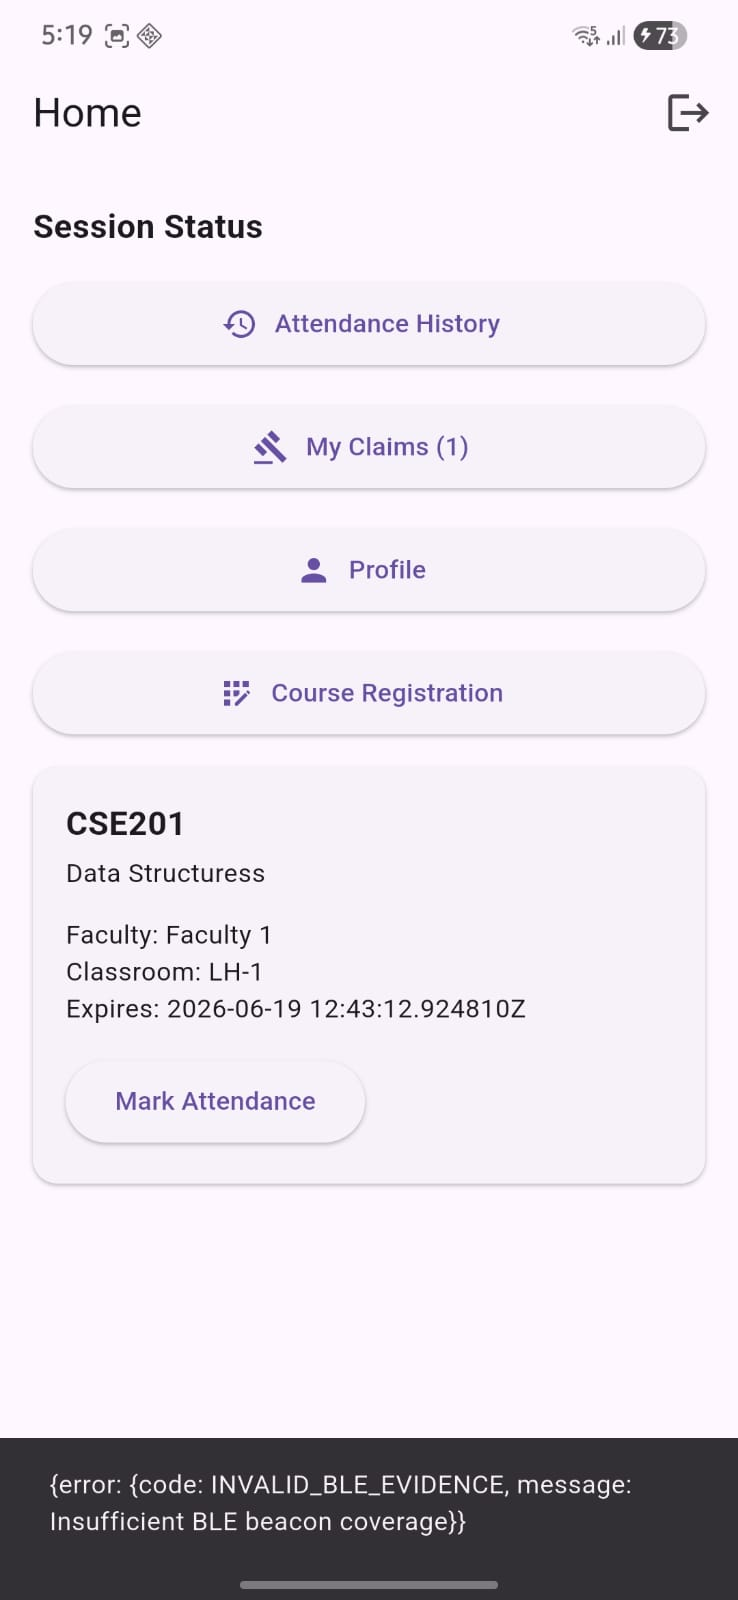
\includegraphics[width=0.7\textwidth]{images/screenshots/security/SEC_04_invalid_ble_evidence.jpeg}
    \caption{Security: Invalid BLE Evidence Rejected}
    \label{fig:appD-sec-04}
\end{figure}

\chapter{Swagger / API Evidence Screenshots}
\label{app:swagger}

This appendix presents Swagger UI screenshots evidencing the REST endpoints summarised in Appendix~A and referenced throughout Chapters~6 and~7, grouped by functional module. These also constitute the underlying evidence for the Swagger API Validation discussion in Section~7.10.

\section{Authentication and Session-Discovery APIs}

\begin{figure}[htbp]
    \centering
    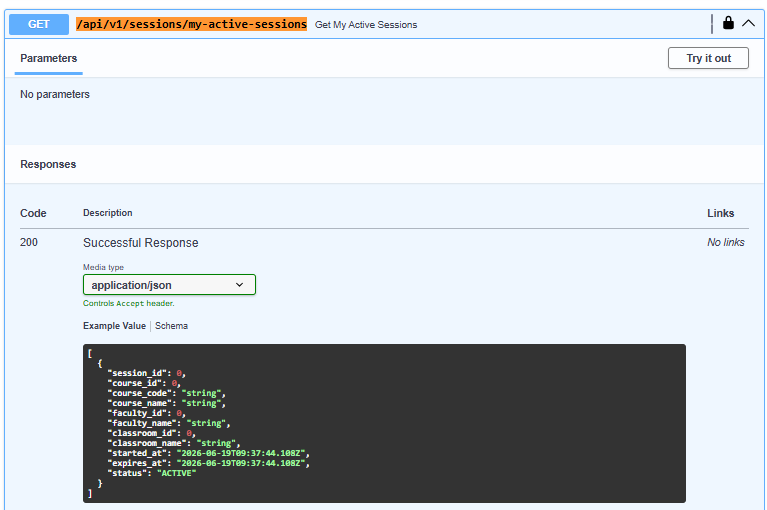
\includegraphics[width=0.8\textwidth]{images/api/active_sessions_api.png}
    \caption{Swagger: Active Sessions API}
    \label{fig:appE-active-sessions}
\end{figure}

\section{Attendance APIs}

\begin{figure}[htbp]
    \centering
    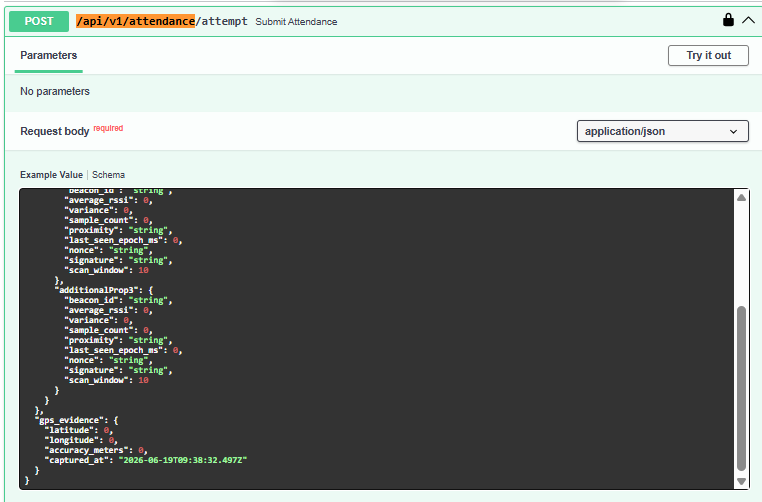
\includegraphics[width=0.8\textwidth]{images/api/submit_attendance_api.png}
    \caption{Swagger: Submit Attendance API}
    \label{fig:appE-submit-attendance}
\end{figure}

\begin{figure}[htbp]
    \centering
    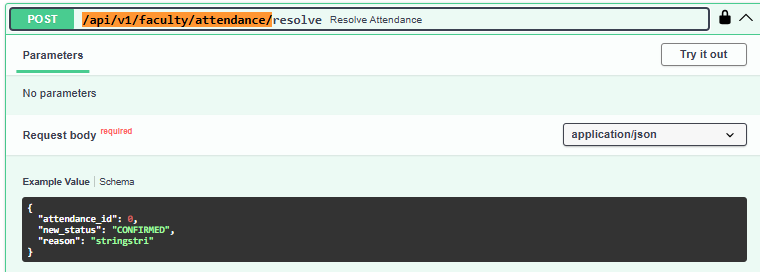
\includegraphics[width=0.8\textwidth]{images/api/review_attendance_api.png}
    \caption{Swagger: Review Attendance API}
    \label{fig:appE-review-attendance}
\end{figure}

\begin{figure}[htbp]
    \centering
    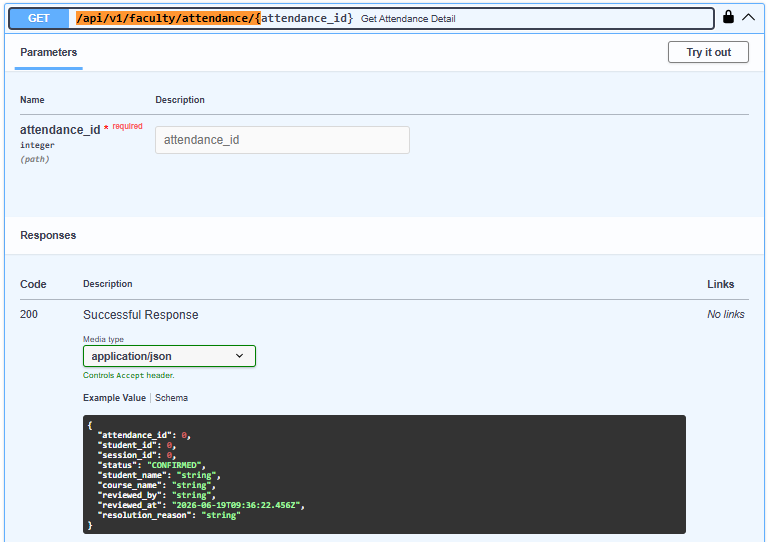
\includegraphics[width=0.8\textwidth]{images/api/reject_attendance_api.png}
    \caption{Swagger: Reject Attendance API}
    \label{fig:appE-reject-attendance}
\end{figure}

\section{Faculty and Session-Management APIs}

\begin{figure}[htbp]
    \centering
    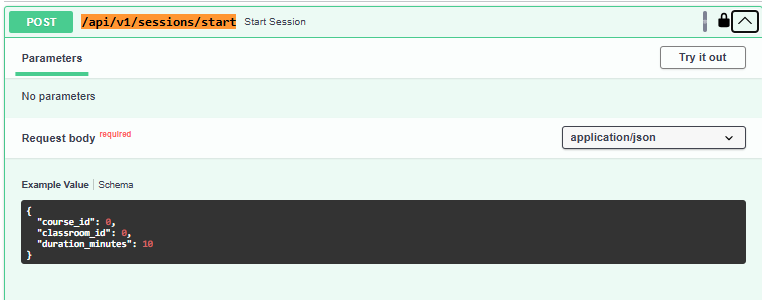
\includegraphics[width=0.8\textwidth]{images/api/start_session_api.png}
    \caption{Swagger: Start Session API}
    \label{fig:appE-start-session}
\end{figure}

\begin{figure}[htbp]
    \centering
    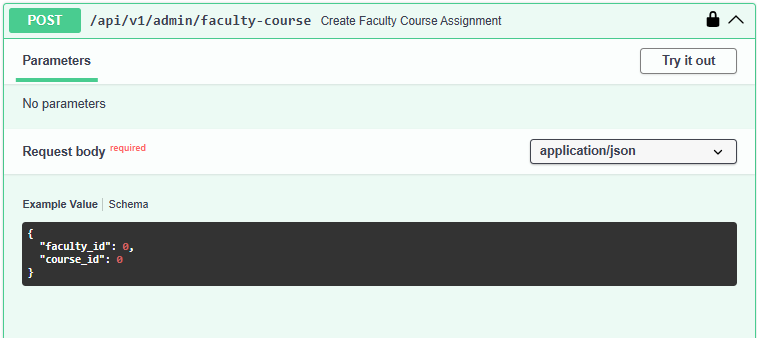
\includegraphics[width=0.8\textwidth]{images/api/assign_faculty_api.png}
    \caption{Swagger: Assign Faculty API}
    \label{fig:appE-assign-faculty}
\end{figure}

\section{Claims APIs}

\begin{figure}[htbp]
    \centering
    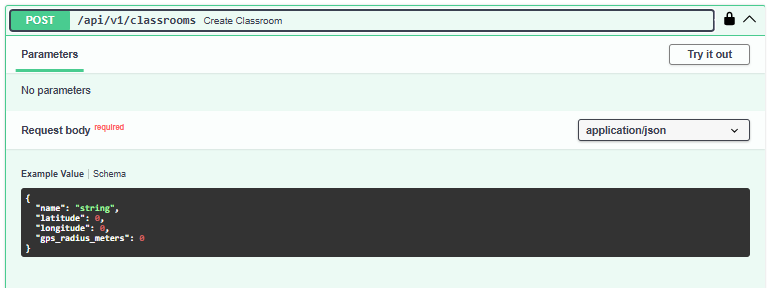
\includegraphics[width=0.8\textwidth]{images/api/create_claim_api.png}
    \caption{Swagger: Create Claim API}
    \label{fig:appE-create-claim}
\end{figure}

\begin{figure}[htbp]
    \centering
    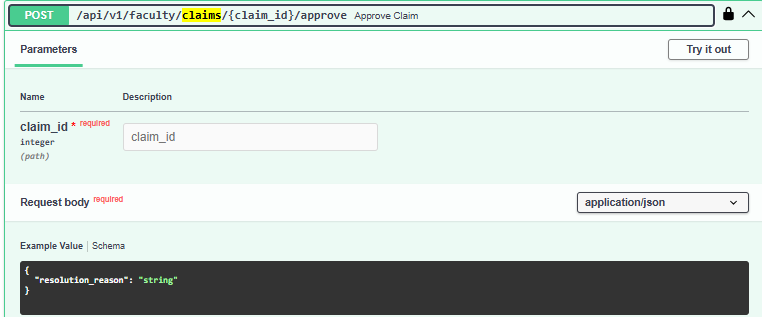
\includegraphics[width=0.8\textwidth]{images/api/approve_claim_api.png}
    \caption{Swagger: Approve Claim API}
    \label{fig:appE-approve-claim}
\end{figure}

\section{Administrative and Beacon-Governance APIs}

\begin{figure}[htbp]
    \centering
    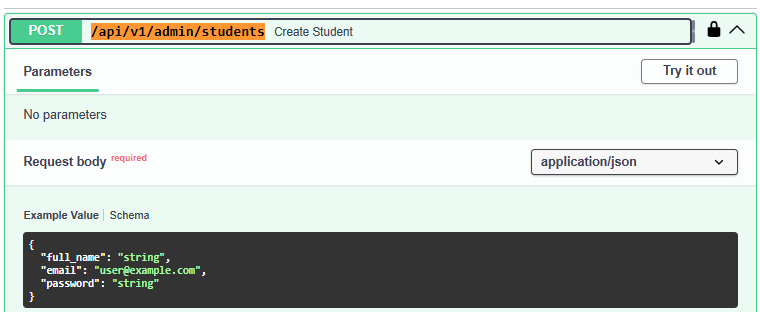
\includegraphics[width=0.8\textwidth]{images/api/create_student_api.png}
    \caption{Swagger: Create Student API}
    \label{fig:appE-create-student}
\end{figure}

\begin{figure}[htbp]
    \centering
    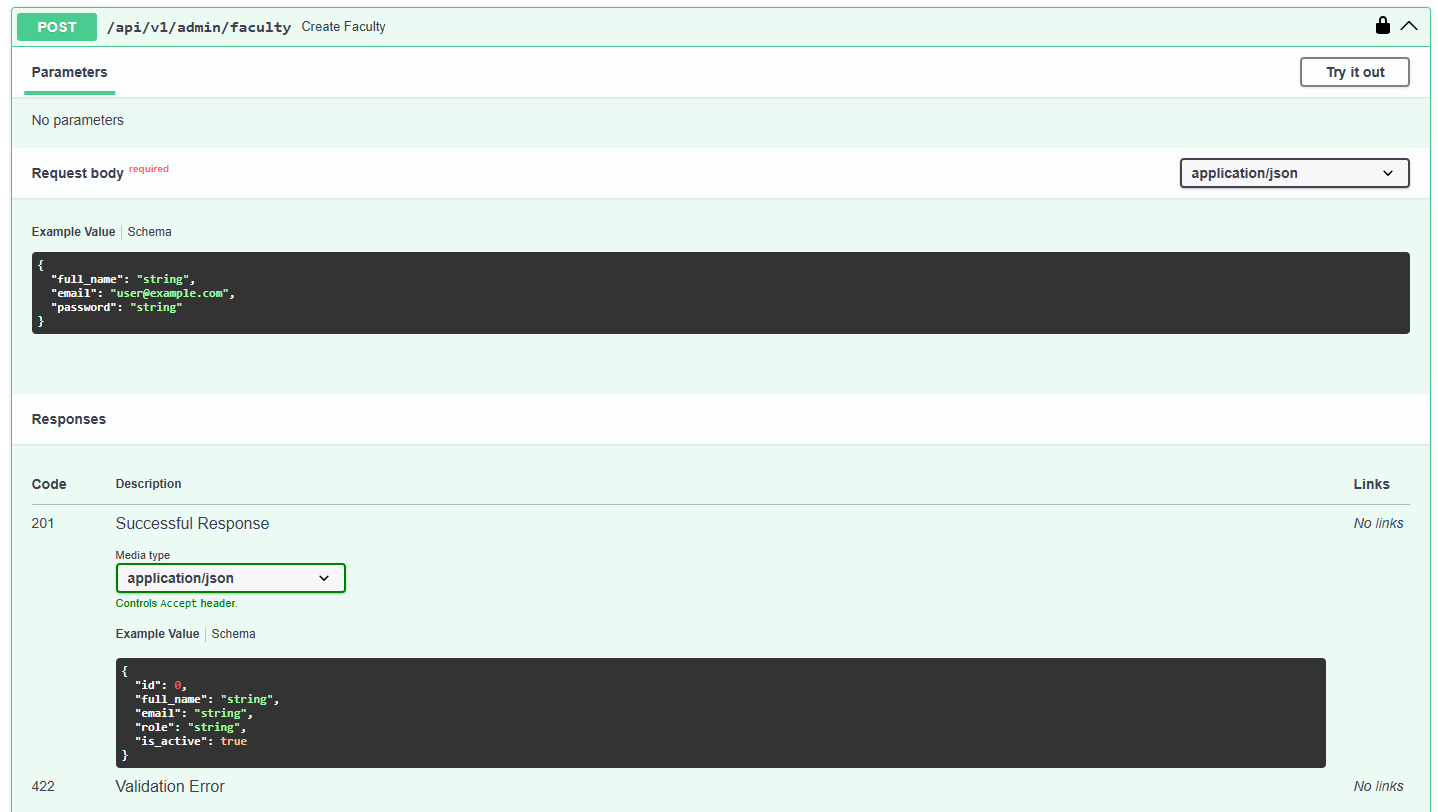
\includegraphics[width=0.8\textwidth]{images/api/create_faculty_api.png}
    \caption{Swagger: Create Faculty API}
    \label{fig:appE-create-faculty}
\end{figure}

\begin{figure}[htbp]
    \centering
    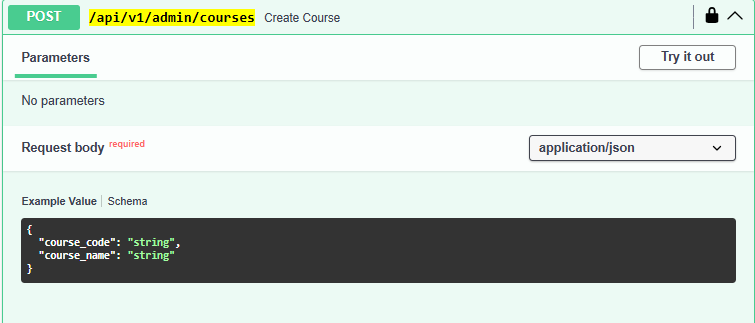
\includegraphics[width=0.8\textwidth]{images/api/create_course_api.png}
    \caption{Swagger: Create Course API}
    \label{fig:appE-create-course}
\end{figure}

\begin{figure}[htbp]
    \centering
    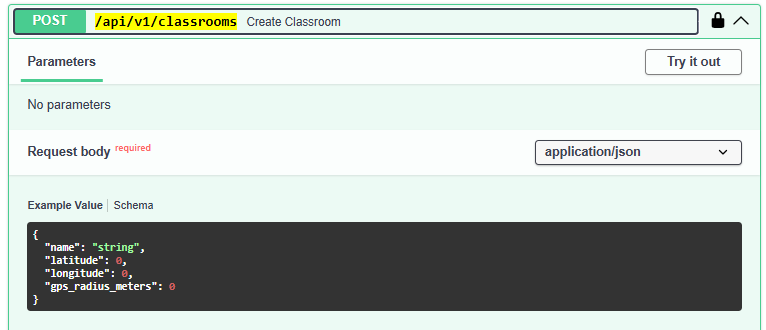
\includegraphics[width=0.8\textwidth]{images/api/create_classroom_api.png}
    \caption{Swagger: Create Classroom API}
    \label{fig:appE-create-classroom}
\end{figure}

\begin{figure}[htbp]
    \centering
    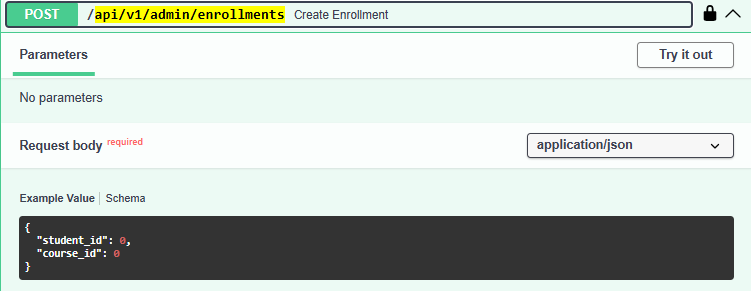
\includegraphics[width=0.8\textwidth]{images/api/enrollment_api.png}
    \caption{Swagger: Enrollment API}
    \label{fig:appE-enrollment}
\end{figure}

\begin{figure}[htbp]
    \centering
    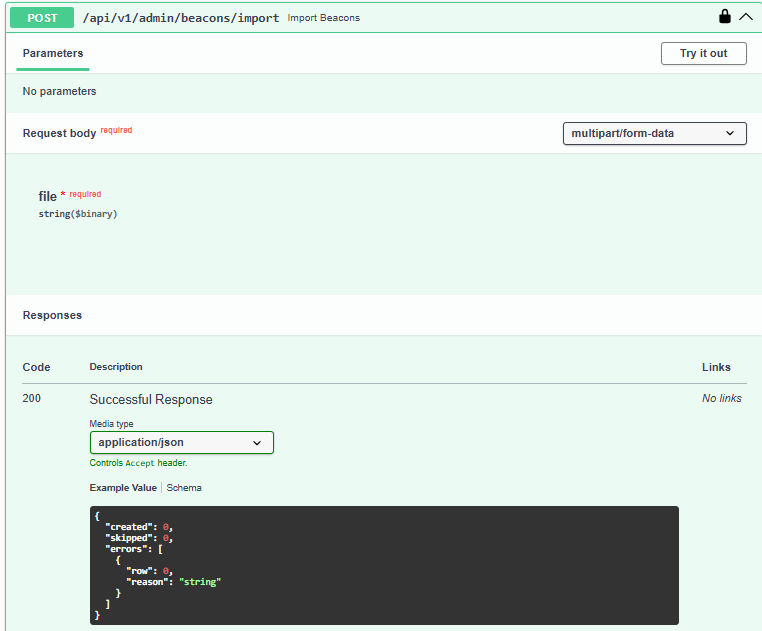
\includegraphics[width=0.8\textwidth]{images/api/assign_beacon_api.png}
    \caption{Swagger: Assign Beacon API}
    \label{fig:appE-assign-beacon}
\end{figure}

\begin{figure}[htbp]
    \centering
    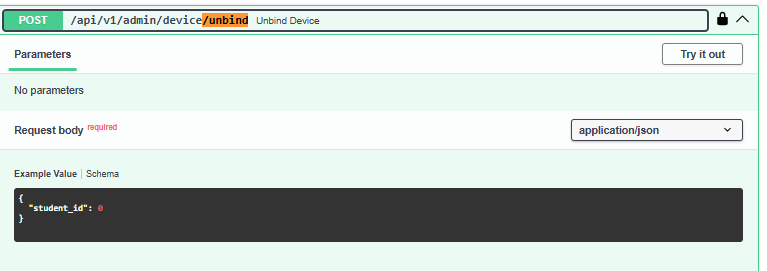
\includegraphics[width=0.8\textwidth]{images/api/device_unbind_api.png}
    \caption{Swagger: Device Unbind API}
    \label{fig:appE-device-unbind}
\end{figure}

\chapter{Database Evidence Screenshots}
\label{app:db-evidence}

This appendix presents pgAdmin database-evidence screenshots corresponding to the schema described in Chapter~5 and Appendix~B, showing table structures, foreign-key relationships, and representative sample data captured directly from the project's database tooling.

\section{Academic Hierarchy Evidence}

\begin{figure}[htbp]
    \centering
    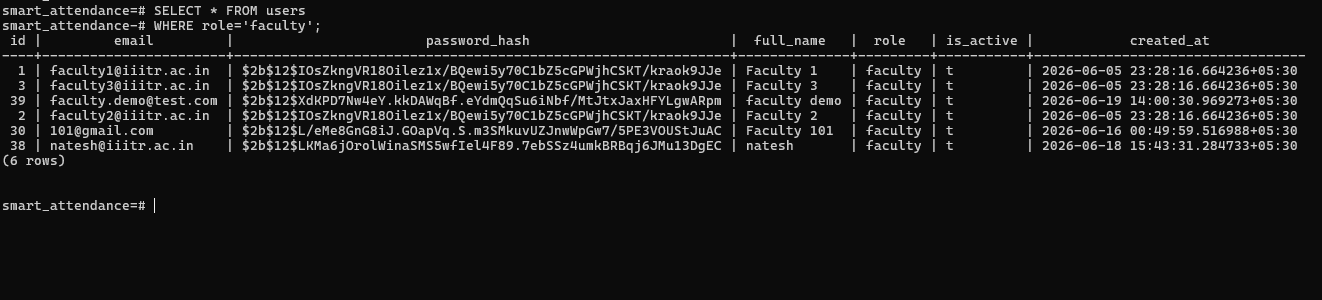
\includegraphics[width=0.8\textwidth]{images/database/faculty_created.png}
    \caption{Database: Faculty Record Created}
    \label{fig:appF-faculty-created}
\end{figure}

\begin{figure}[htbp]
    \centering
    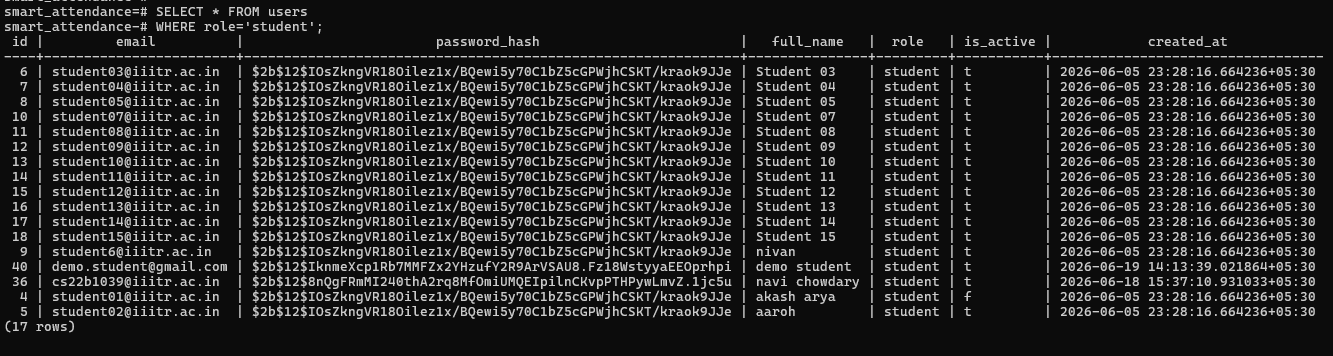
\includegraphics[width=0.8\textwidth]{images/database/student_created.png}
    \caption{Database: Student Record Created}
    \label{fig:appF-student-created}
\end{figure}

\begin{figure}[htbp]
    \centering
    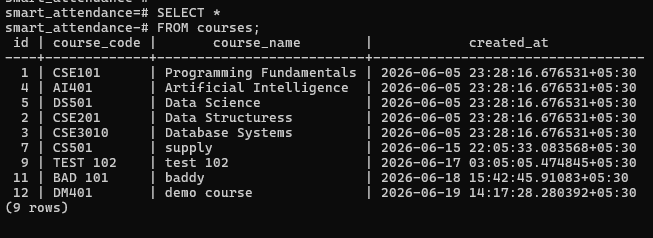
\includegraphics[width=0.8\textwidth]{images/database/course_created.png}
    \caption{Database: Course Record Created}
    \label{fig:appF-course-created}
\end{figure}

\begin{figure}[htbp]
    \centering
    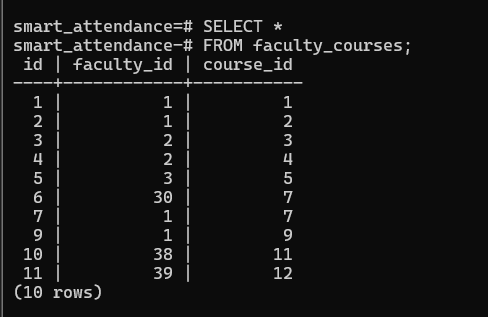
\includegraphics[width=0.8\textwidth]{images/database/faculty_assignment.png}
    \caption{Database: Faculty-Course Assignment}
    \label{fig:appF-faculty-assignment}
\end{figure}

\begin{figure}[htbp]
    \centering
    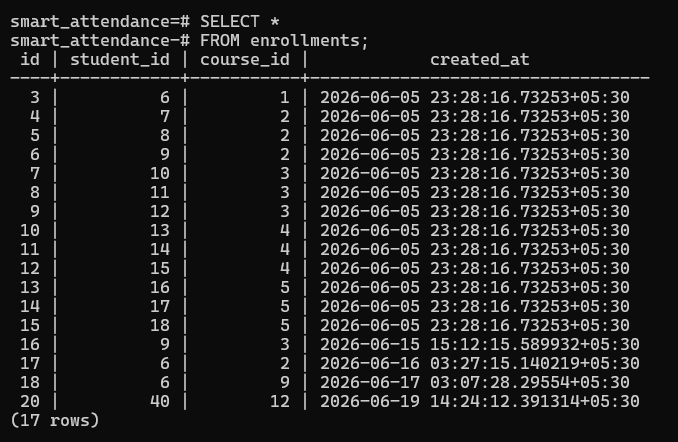
\includegraphics[width=0.8\textwidth]{images/database/student_enrollment.png}
    \caption{Database: Student Enrollment}
    \label{fig:appF-student-enrollment}
\end{figure}

\begin{figure}[htbp]
    \centering
    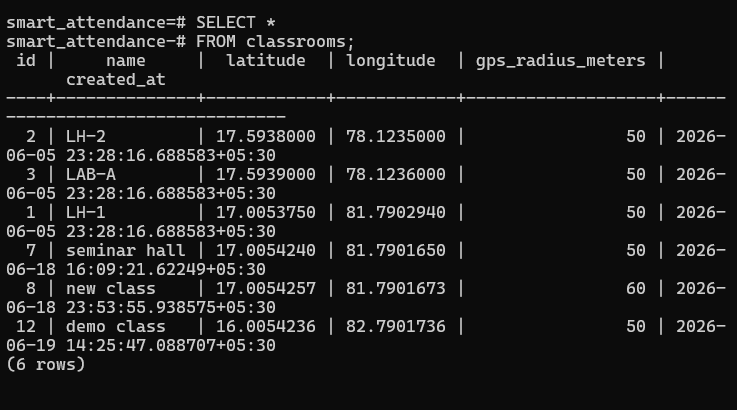
\includegraphics[width=0.8\textwidth]{images/database/classroom_created.png}
    \caption{Database: Classroom Record Created}
    \label{fig:appF-classroom-created}
\end{figure}

\begin{figure}[htbp]
    \centering
    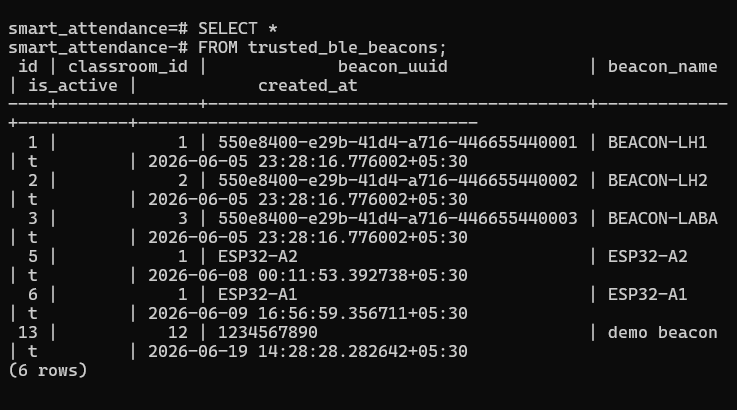
\includegraphics[width=0.8\textwidth]{images/database/beacon_assignment.png}
    \caption{Database: Beacon Assignment}
    \label{fig:appF-beacon-assignment}
\end{figure}

\section{Attendance and Evidence Tables}

\begin{figure}[htbp]
    \centering
    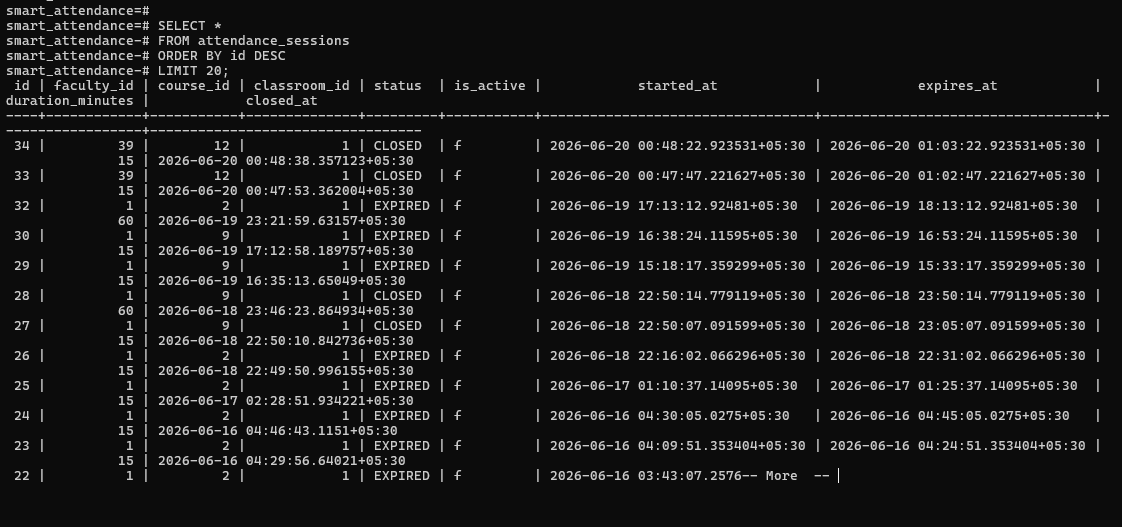
\includegraphics[width=0.8\textwidth]{images/database/attendance_session.png}
    \caption{Database: Attendance Session Record}
    \label{fig:appF-attendance-session}
\end{figure}

\begin{figure}[htbp]
    \centering
    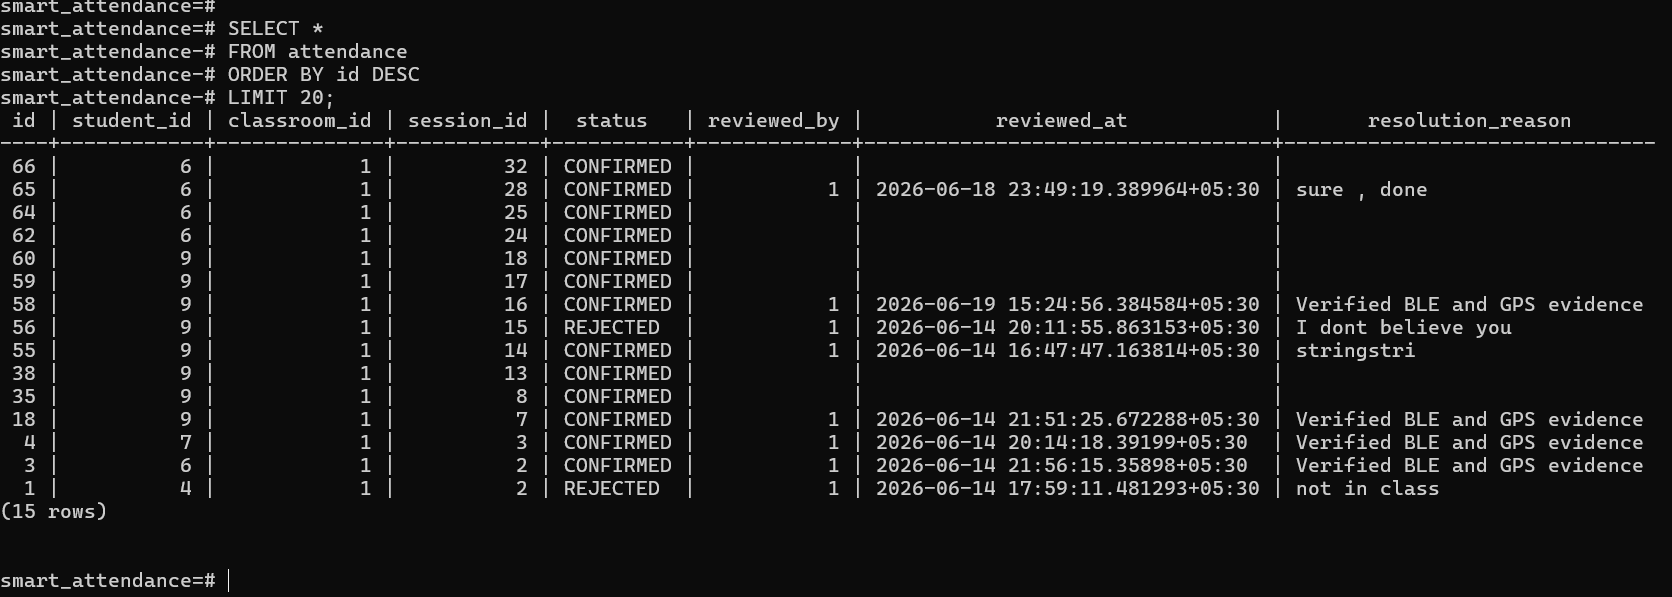
\includegraphics[width=0.8\textwidth]{images/database/attendance_record.png}
    \caption{Database: Attendance Record}
    \label{fig:appF-attendance-record}
\end{figure}

\begin{figure}[htbp]
    \centering
    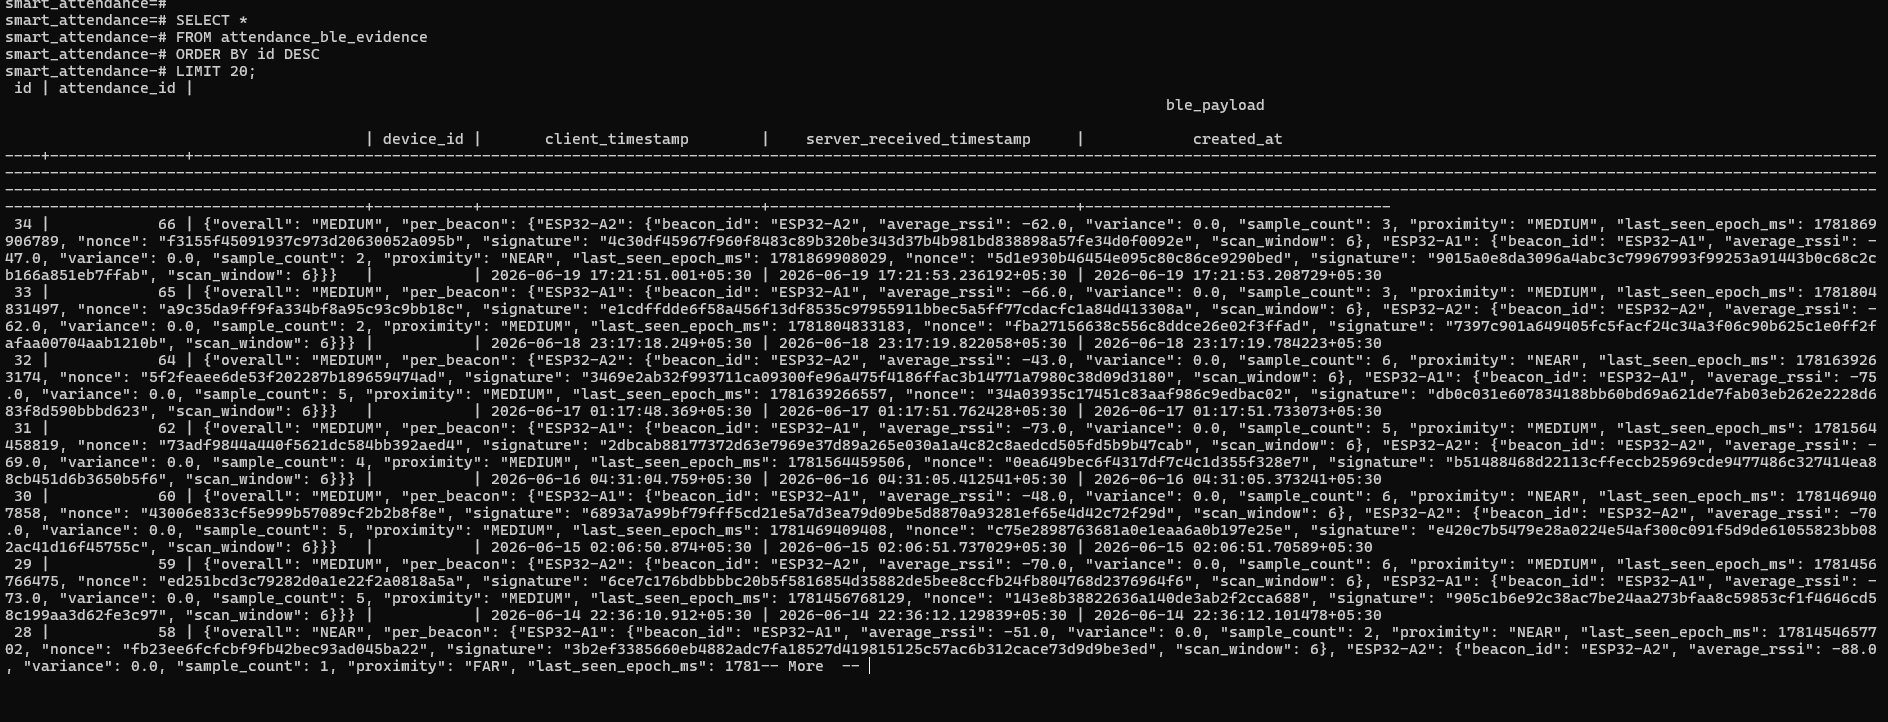
\includegraphics[width=0.8\textwidth]{images/database/attendance_ble_evidence.png}
    \caption{Database: BLE Evidence Record}
    \label{fig:appF-ble-evidence}
\end{figure}

\begin{figure}[htbp]
    \centering
    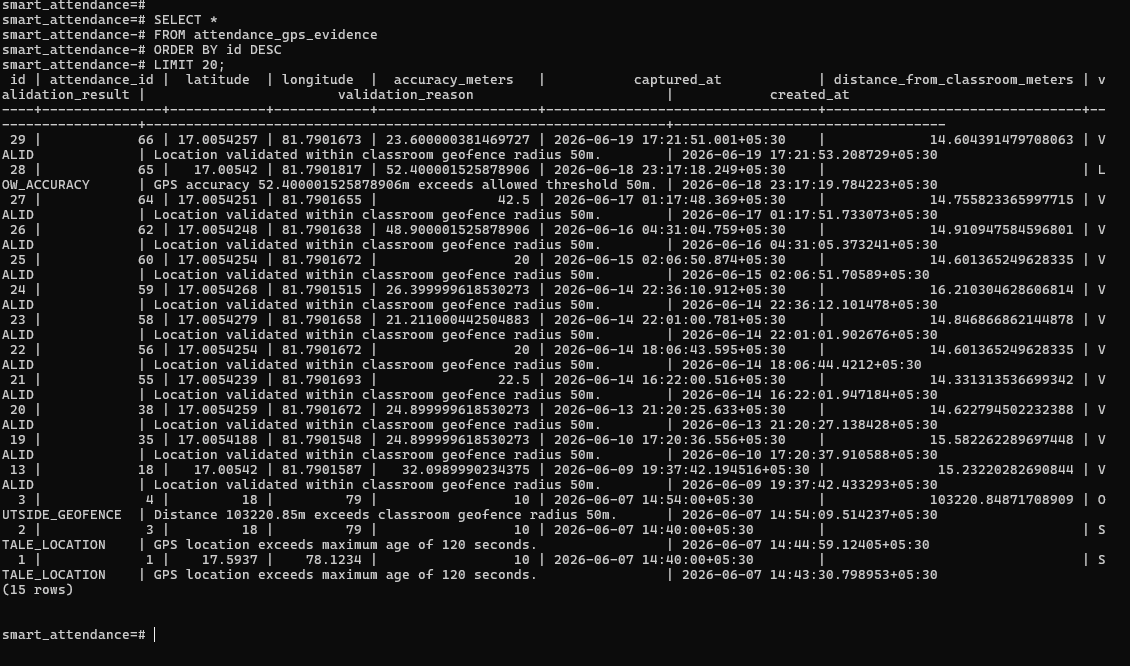
\includegraphics[width=0.8\textwidth]{images/database/attendance_gps_evidence.png}
    \caption{Database: GPS Evidence Record}
    \label{fig:appF-gps-evidence}
\end{figure}

\begin{figure}[htbp]
    \centering
    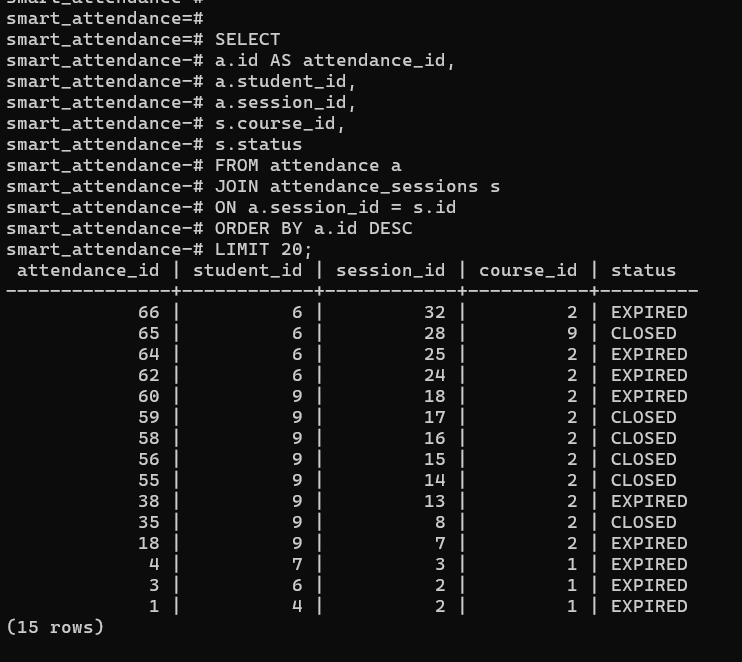
\includegraphics[width=0.8\textwidth]{images/database/attendance_session_integrity.png}
    \caption{Database: Attendance Session Integrity Constraint}
    \label{fig:appF-session-integrity}
\end{figure}

\begin{figure}[htbp]
    \centering
    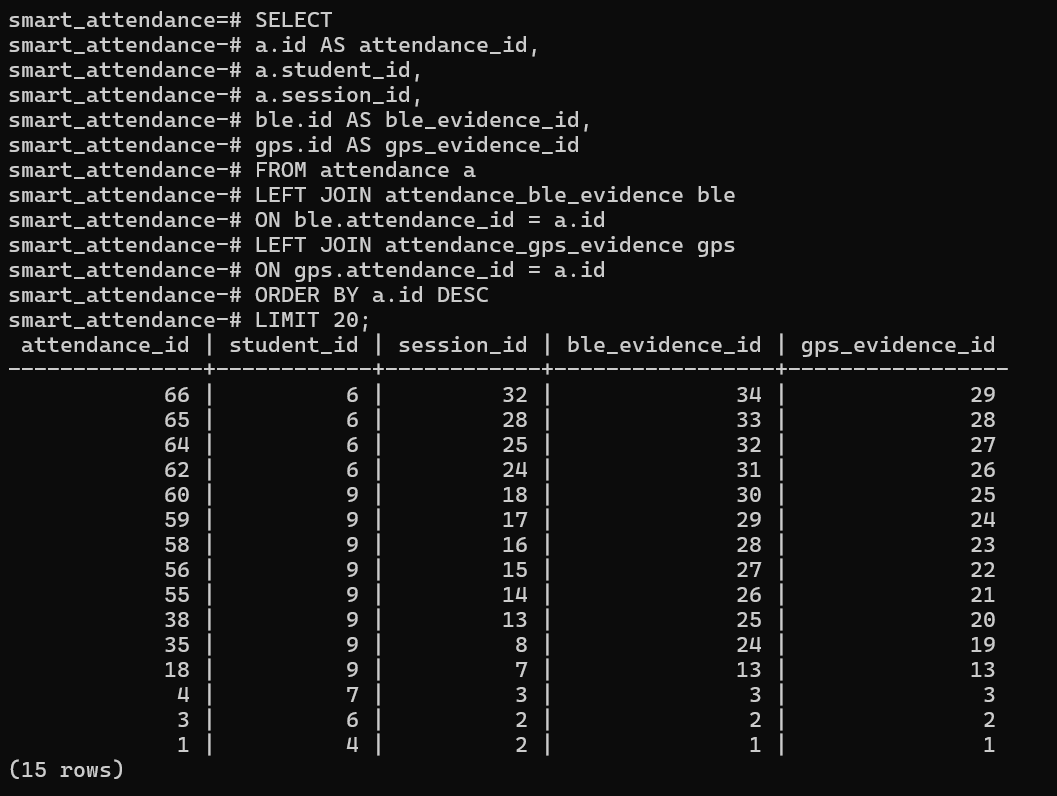
\includegraphics[width=0.8\textwidth]{images/database/full_attendance_chain.png}
    \caption{Database: Full Attendance Chain (Joined Evidence View)}
    \label{fig:appF-full-chain}
\end{figure}

\section{Claims Evidence}

\begin{figure}[htbp]
    \centering
    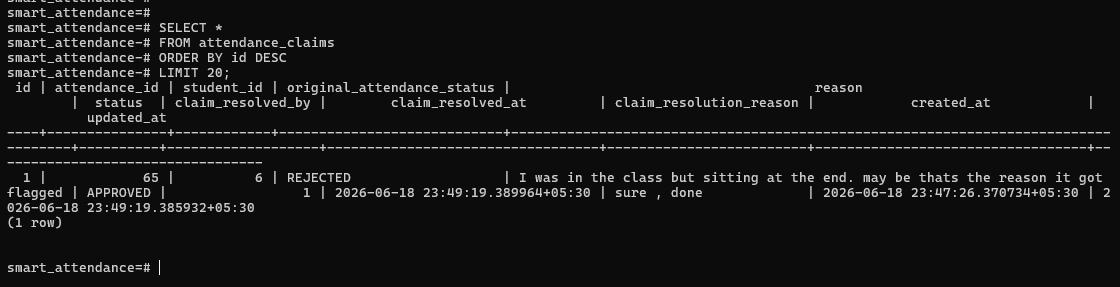
\includegraphics[width=0.8\textwidth]{images/database/claim_record.png}
    \caption{Database: Claim Record}
    \label{fig:appF-claim-record}
\end{figure}

\begin{figure}[htbp]
    \centering
    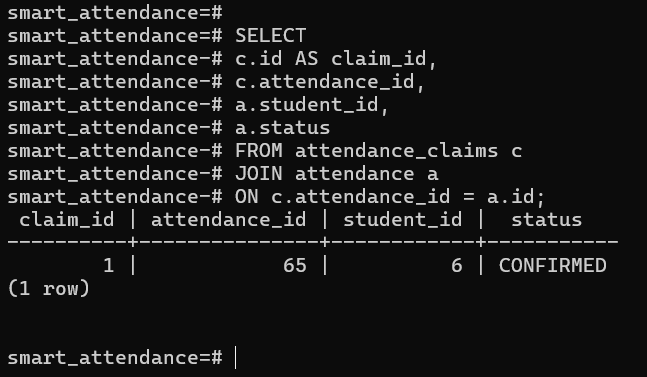
\includegraphics[width=0.8\textwidth]{images/database/claim_attendance_integrity.png}
    \caption{Database: Claim-Attendance Integrity Constraint}
    \label{fig:appF-claim-integrity}
\end{figure}

\section{Security and Governance Evidence}

\begin{figure}[htbp]
    \centering
    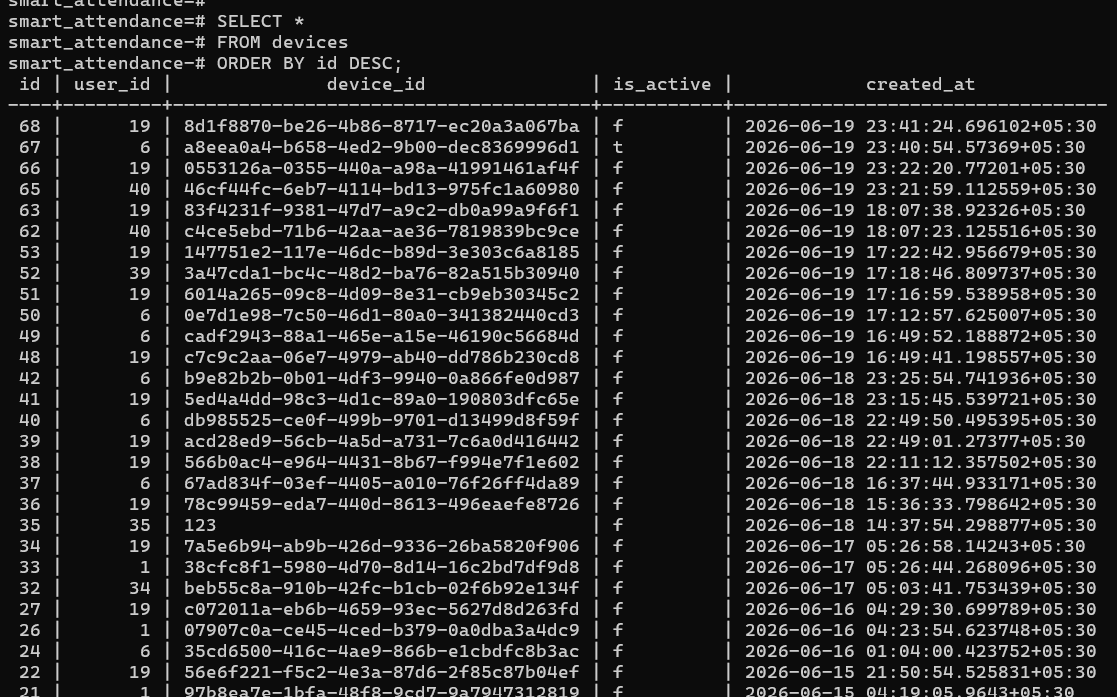
\includegraphics[width=0.8\textwidth]{images/database/device_binding.png}
    \caption{Database: Device Binding Record}
    \label{fig:appF-device-binding}
\end{figure}

\begin{figure}[htbp]
    \centering
    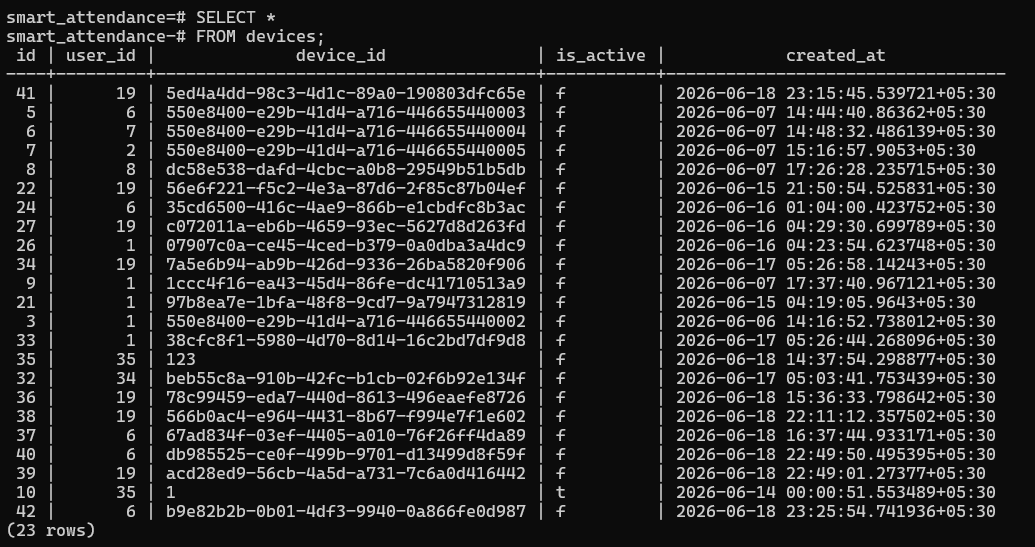
\includegraphics[width=0.8\textwidth]{images/database/device_unbind.png}
    \caption{Database: Device Unbind Record}
    \label{fig:appF-device-unbind}
\end{figure}

\begin{figure}[htbp]
    \centering
    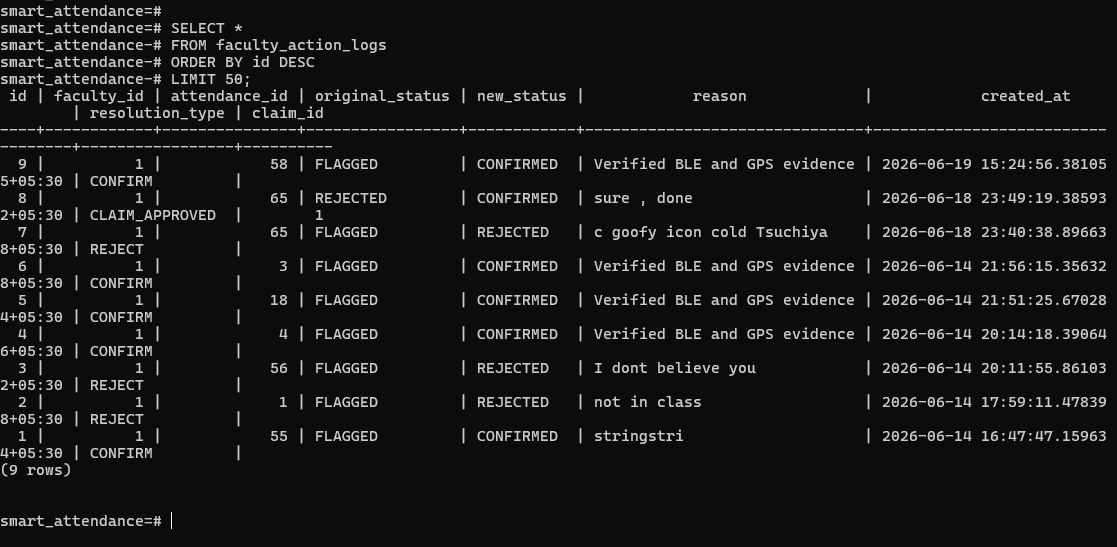
\includegraphics[width=0.8\textwidth]{images/database/faculty_action_log.png}
    \caption{Database: Faculty Action Log}
    \label{fig:appF-action-log}
\end{figure}

\begin{figure}[htbp]
    \centering
    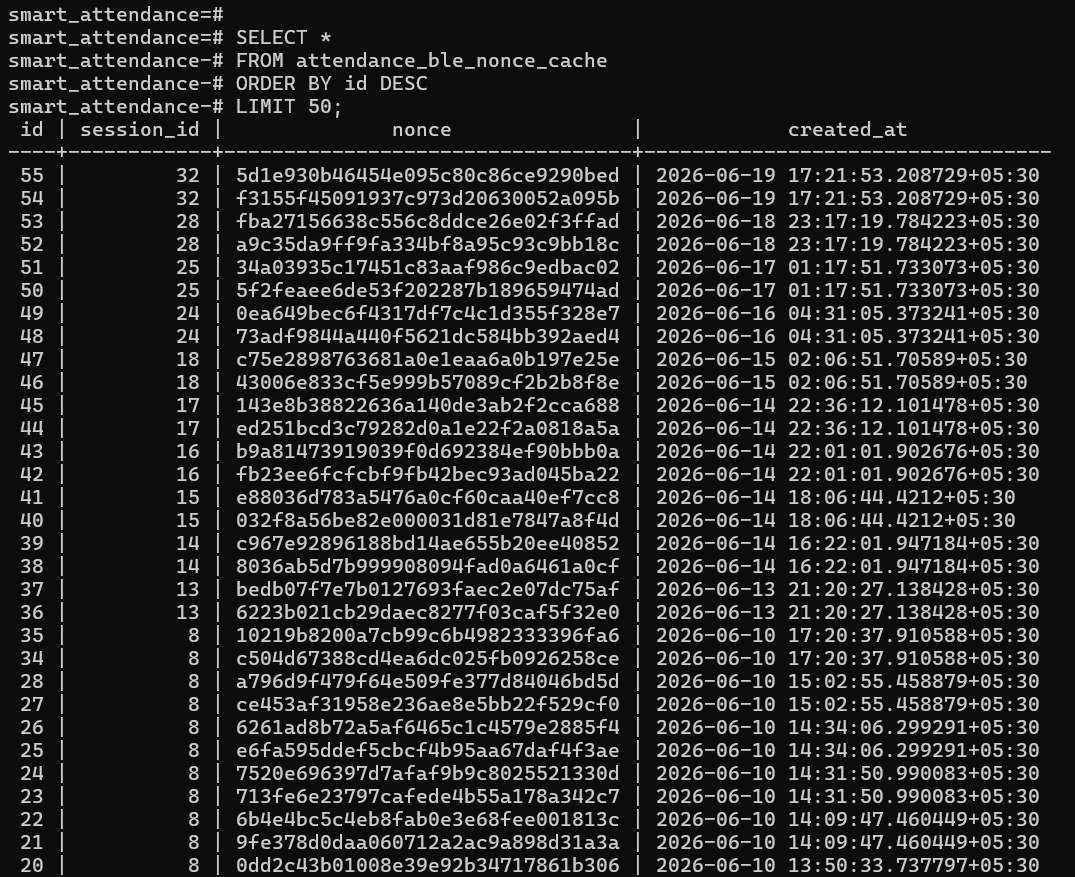
\includegraphics[width=0.8\textwidth]{images/database/ble_nonce_cache.png}
    \caption{Database: BLE Nonce Cache}
    \label{fig:appF-nonce-cache}
\end{figure}

\section{Registration Workflow Evidence}

\begin{figure}[htbp]
    \centering
    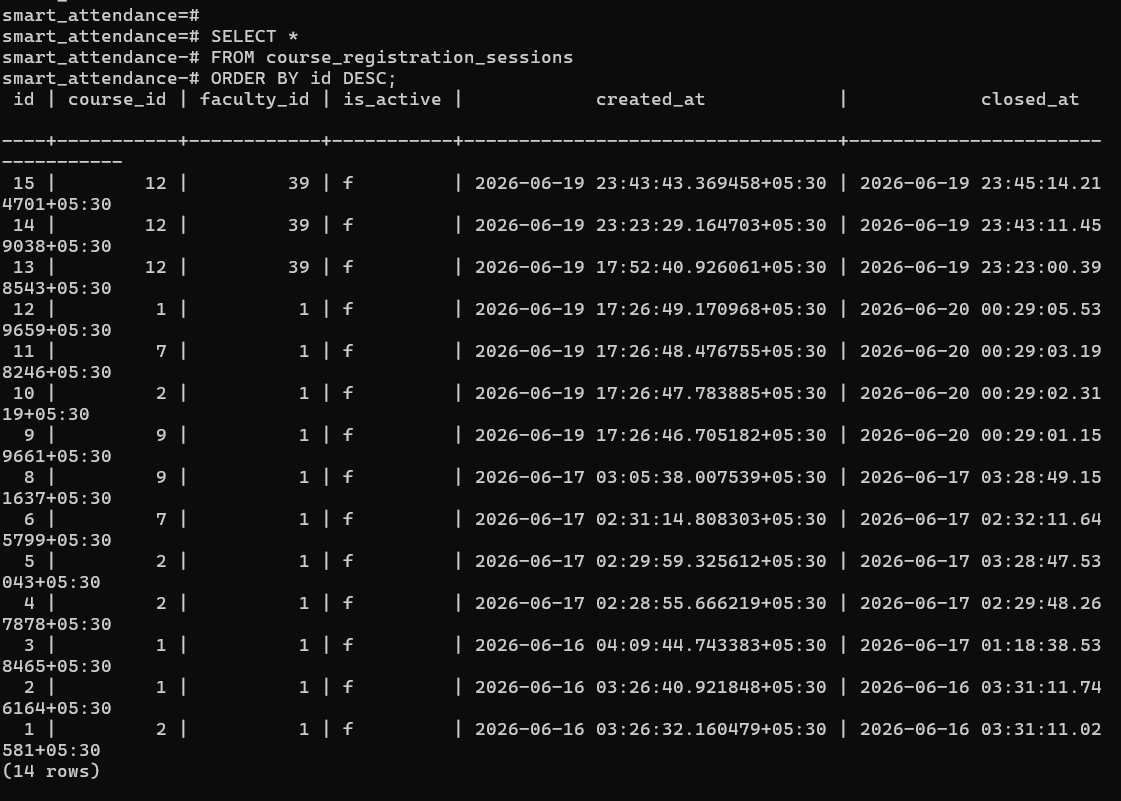
\includegraphics[width=0.8\textwidth]{images/database/registration_sessions.png}
    \caption{Database: Registration Sessions}
    \label{fig:appF-registration-sessions}
\end{figure}

\begin{figure}[htbp]
    \centering
    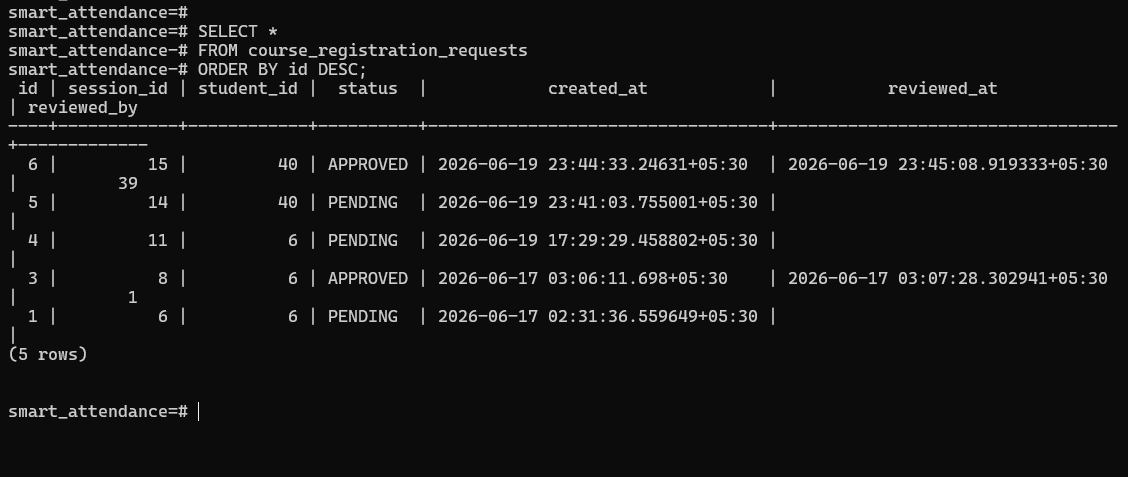
\includegraphics[width=0.8\textwidth]{images/database/registration_requests.png}
    \caption{Database: Registration Requests}
    \label{fig:appF-registration-requests}
\end{figure}

\chapter{Sample Payloads and API Messages}
\label{app:payloads}

This appendix reproduces representative request and response payloads referenced throughout Chapters~4 and~6, for readers who want to see the evidence formats described in the text written out explicitly. All values shown are illustrative; secrets and tokens are masked or truncated.

\noindent\textbf{Sample BLE Beacon Payload (Section 4.10)}

\begin{lstlisting}
{
  "beacon_id": "ESP32-A1",
  "nonce": "9f3e1c2a7b5d",
  "timestamp": 1750000000,
  "signature": "3f7a9c1e...b2"
}
\end{lstlisting}

\noindent\textbf{Sample JWT Payload (masked)}

\begin{lstlisting}
{
  "sub": "user_1042",
  "role": "STUDENT",
  "device_id": "dev_88a2...",
  "iat": 1750000000,
  "exp": 1750003600
}
\end{lstlisting}

\textit{Note: the value shown is the decoded payload segment of the token for illustration only; the actual JWT transmitted over the wire is a signed, encoded string and the signing key is never exposed to the client.}

\noindent\textbf{Sample Attendance Submission -- Request}

\begin{lstlisting}
POST /attendance/submit
{
  "session_id": 4821,
  "ble_evidence": {
    "beacon_id": "ESP32-A1",
    "nonce": "9f3e1c2a7b5d",
    "timestamp": 1750000000,
    "signature": "3f7a9c1e...b2",
    "rssi": -58
  },
  "gps_evidence": {
    "latitude": 17.3850,
    "longitude": 78.4867,
    "accuracy_m": 6.2
  }
}
\end{lstlisting}

\noindent\textbf{Sample Attendance Submission -- Response}

\begin{lstlisting}
{
  "attempt_id": 19553,
  "status": "CONFIRMED",
  "ble_result": "VALID",
  "gps_result": "VALID",
  "submitted_at": "2026-02-14T09:31:02Z"
}
\end{lstlisting}

\noindent\textbf{Sample Claim Submission -- Request}

\begin{lstlisting}
POST /claims
{
  "attempt_id": 19560,
  "reason": "I was present in the classroom; GPS accuracy was poor near the window seating area."
}
\end{lstlisting}

\fi
\chapter{Glossary}
\label{app:glossary}

\begin{description}[style=multiline, leftmargin=3cm]
\item[Attendance Attempt] A single recorded submission of attendance evidence by a student against one attendance session.
\item[Beacon] An ESP32-based hardware device installed in a classroom that periodically broadcasts a signed BLE payload used as proximity evidence.
\item[Claim] A student-initiated request to contest a REJECTED attendance attempt, resolved by the owning faculty member.
\item[Device Binding] The enforced association between a student's account and a single registered physical device.
\item[Evidence Fusion] The process of combining BLE and GPS evidence into a single attendance decision rather than treating either channel as decisive on its own.
\item[Geofence] A virtual boundary, defined by a centre coordinate and radius, against which a device's reported GPS position is checked.
\item[Nonce] A single-use, randomly generated value included in each beacon payload to prevent the same broadcast from being replayed and accepted twice.
\item[Replay Attack] An attack in which previously captured, legitimate evidence (for example, a BLE payload) is recorded and resubmitted later to fraudulently register attendance.
\end{description}

\fi
\end{document}
